% \DeclareDocumentMetadata {lang=en-US}

% xmp metadata for pdf
% Originally used \usepackage[a-2a]{pdfx}
% \usepackage{hyperxmp} replaced it
% \RequirePackage{pdfmanagement-testphase} replaced it
% \PassOptionsToPackage{enable-debug,check-declarations}{expl3} broke with version 0.9 of tagpdf
% \ExplSyntaxOn no need for these 3 lines because metadata can handle it
% \pdfmanagement_add:nnn{Catalog}{Lang}{(enUS)} enUS is wrong, should be en-US
% \ExplSyntaxOff

\documentclass[11pt,
  english,
  letterpaper,
]{article}
\usepackage{sa4ss}
\usepackage{amsmath,amssymb,array}
\usepackage{booktabs}

% From tagged-template.latex
\usepackage{lmodern}
\usepackage{ifxetex,ifluatex}
\ifnum 0\ifxetex 1\fi\ifluatex 1\fi=0 % if pdftex
  \usepackage[T1]{fontenc}
  \usepackage[utf8]{inputenc}
  \usepackage{textcomp} % provide euro and other symbols
\else % if luatex or xetex
  \usepackage{unicode-math}
  \defaultfontfeatures{Scale=MatchLowercase}
  \defaultfontfeatures[\rmfamily]{Ligatures=TeX,Scale=1}
\fi

% Use upquote if available, for straight quotes in verbatim environments
\IfFileExists{upquote.sty}{\usepackage{upquote}}{}
\IfFileExists{microtype.sty}{% use microtype if available
  \usepackage[]{microtype}
  \UseMicrotypeSet[protrusion]{basicmath} % disable protrusion for tt fonts
}{}
\makeatletter
\@ifundefined{KOMAClassName}{% if non-KOMA class
  \IfFileExists{parskip.sty}{%
    \usepackage{parskip}
  }{% else
    \setlength{\parindent}{0pt}
    \setlength{\parskip}{6pt plus 2pt minus 1pt}}
}{% if KOMA class
  \KOMAoptions{parskip=half}}
\makeatother
\usepackage{xcolor}
\IfFileExists{xurl.sty}{\usepackage{xurl}}{} % add URL line breaks if available
\hypersetup{
  pdftitle={Status of Black Rockfish (Sebastes melanops) in 2023 in state and federal waters off Oregon},
  pdflang={en},
  hidelinks,
  pdfcreator={LaTeX via pandoc}}
\urlstyle{same} % disable monospaced font for URLs
\usepackage{longtable}
% Correct order of tables after \paragraph or \subparagraph
\usepackage{etoolbox}
\makeatletter
\patchcmd\longtable{\par}{\if@noskipsec\mbox{}\fi\par}{}{}
\makeatother
% Allow footnotes in longtable head/foot
\IfFileExists{footnotehyper.sty}{\usepackage{footnotehyper}}{\usepackage{footnote}}
\makesavenoteenv{longtable}
\usepackage{graphicx}
\makeatletter
\def\maxwidth{\ifdim\Gin@nat@width>\linewidth\linewidth\else\Gin@nat@width\fi}
\def\maxheight{\ifdim\Gin@nat@height>\textheight\textheight\else\Gin@nat@height\fi}
\makeatother
% Scale images if necessary, so that they will not overflow the page
% margins by default, and it is still possible to overwrite the defaults
% using explicit options in \includegraphics[width, height, ...]{}
\setkeys{Gin}{width=\maxwidth,height=\maxheight,keepaspectratio}
% Set default figure placement to htbp
\makeatletter
\def\fps@figure{htbp}
\makeatother
\setlength{\emergencystretch}{3em} % prevent overfull lines
\providecommand{\tightlist}{%
  \setlength{\itemsep}{0pt}\setlength{\parskip}{0pt}}
\setcounter{secnumdepth}{5}
\ifxetex
  % Load polyglossia as late as possible: uses bidi with RTL langages (e.g. Hebrew, Arabic)
  \usepackage{polyglossia}
  \setmainlanguage[]{}
\else
  \usepackage[shorthands=off,main=english]{babel}
\fi

%Define cslreferences environment, required by pandoc 2.8
%https://github.com/rstudio/rmarkdown/issues/1649
\newlength{\csllabelwidth}
\setlength{\csllabelwidth}{3em}
\newlength{\cslhangindent}
\setlength{\cslhangindent}{1.5em}
% for Pandoc 2.8 to 2.10.1
\newenvironment{cslreferences}%
  {}%
  {\par}
% For Pandoc 2.11+
\newenvironment{CSLReferences}[2] % #1 hanging-ident, #2 entry spacing
 {% don't indent paragraphs
  \setlength{\parindent}{0pt}
  % turn on hanging indent if param 1 is 1
  \ifodd #1 \everypar{\setlength{\hangindent}{\cslhangindent}}\ignorespaces\fi
  % set entry spacing
  \ifnum #2 > 0
  \setlength{\parskip}{#2\baselineskip}
  \fi
 }%
 {}
\usepackage{calc}  % for \widthof, \maxof in minipage
\newcommand{\CSLBlock}[1]{#1\hfill\break}
\newcommand{\CSLLeftMargin}[1]{\parbox[t]{\csllabelwidth}{#1}}
\newcommand{\CSLRightInline}[1]{\parbox[t]{\linewidth - \csllabelwidth}{#1}\break}
\newcommand{\CSLIndent}[1]{\hspace{\cslhangindent}#1}


\providecommand{\tightlist}{%
  \setlength{\itemsep}{0pt}\setlength{\parskip}{0pt}}


\date{}
\newcommand{\trTitle}{Status of Black Rockfish (\emph{Sebastes melanops}) in 2023 in state and federal waters off Oregon}
\newcommand{\trYear}{2023}
\newcommand{\trMonth}{June}
\newcommand{\trAuthsLong}{truetruetruetrue}
\newcommand{\trAuthsBack}{Cope, J.M., A.D. Whitman, A.M. Berger, L.R. Rasmuson}
\newcommand{\trCitation}{
\begin{hangparas}{1em}{1}
\trAuthsBack{}. \trYear{}. \trTitle{}. \glsentrylong{pfmc}, Portland, Oregon. \pageref{LastPage}{}\,p.
\end{hangparas}}

\newcommand\includegraphicsifexists[2][width=\linewidth]{\IfFileExists{#2}{\includegraphics[#1]{#2}}{}}

\begin{document}

%%%%% Frontmatter %%%%%

% Footnote symbols in front matter
\renewcommand*{\thefootnote}{\fnsymbol{footnote}}

\small
\thispagestyle{empty}
\pagenumbering{roman}
\noindent
\begin{center}
\title{Status of Black Rockfish (\emph{Sebastes melanops}) in 2023 in state and federal waters off Oregon}
% \textnormal{\MakeTextUppercase{\trTitle{}}}
\vspace{1.5cm}
{\Large\textbf\newline{Status of Black Rockfish (\emph{Sebastes melanops}) in 2023 in state and federal waters off Oregon}}

\includegraphicsifexists[width=4in]{figure_title.png}
\vfill
by\\
Jason M. Cope\textsuperscript{1}\\
Alison D. Whitman\textsuperscript{2}\\
Aaron M. Berger\textsuperscript{1}\\
Leif R. Rasmuson\textsuperscript{2}\vfill
\textsuperscript{1}Northwest Fisheries Science Center, U.S. Department of Commerce, National Oceanic and Atmospheric Administration, National Marine Fisheries Service, 2725 Montlake Boulevard East, Seattle, Washington 98112\\
\textsuperscript{2}Oregon Department of Fish and Wildlife, 2040 Southeast Marine Science Drive, Newport, Oregon 97365\vfill
\trMonth{} \trYear{}
\end{center}
\clearpage

% Fourth page: Colophon
\thispagestyle{empty}
\vspace*{\fill}
\begin{center}
\copyright{} \glsentrylong{pfmc}, \trYear{}\\
\end{center}
\par
\bigskip
\noindent
Correct citation for this publication:
\bigskip
\par
\trCitation{}
\clearpage

% Add TOC to pdf bookmarks (clickable pdf)
\pdfbookmark[1]{\contentsname}{toc}

% Table of contents page, lists of figures and tables
\tableofcontents\clearpage
\label{TRlastRoman}
\clearpage

% Table of contents
\newpage
\thispagestyle{empty} % to remove page number

% Settings for the main document
\pagenumbering{arabic}  % Regular page numbers
\pagestyle{plain}  % No page number on first page of main document, use 'empty'
\renewcommand*{\thefootnote}{\arabic{footnote}}  % Back to numeric footnotes
\setcounter{footnote}{0}  % And start at 1
\renewcommand{\headrulewidth}{0.5pt}
\renewcommand{\footrulewidth}{0.5pt}
%\pagestyle{fancy}\fancyhead[c]{Draft: Do not cite or circulate}

\newcommand{\lt}{\ensuremath <}
\newcommand{\gt}{\ensuremath >}

\vspace{500cm}

\hypertarget{disclaimer}{%
\section*{Disclaimer}\label{disclaimer}}
\addcontentsline{toc}{section}{Disclaimer}

\textbf{These materials do not constitute a formal publication and are for information only. They are in a pre-review, pre-decisional state and should not be formally cited or reproduced. They are to be considered provisional and do not represent any determination or policy of NOAA or the Department of Commerce.}

\pagebreak
\pagenumbering{roman}
\setcounter{page}{1}

\renewcommand{\thetable}{\roman{table}}
\renewcommand{\thefigure}{\roman{figure}}

\setlength\parskip{0.5em plus 0.1em minus 0.2em}

\hypertarget{one-page-summary}{%
\section*{One Page Summary}\label{one-page-summary}}
\addcontentsline{toc}{section}{One Page Summary}

\begin{itemize}

\item This assessment for Black Rockfish in Oregon waters incorporates a wide range of data sources: removals from two commercial and two recreational fleets; three fishery-dependent indices of abundance, three fishery-independent indices of abundance, length and conditional age-at-length composition data for several fisheries and surveys; information on weight-at-length, maturity-at-length, and fecundity-at-length; information on natural mortality and the steepness of the Beverton-Holt stock-recruitment relationship; and estimates of ageing error.

\item The addition of a new coastwide acoustic-visual survey (conducted in 2021) was incorporated into the base model to provide direct information on overall population scale and to anchor related information on scale from earlier (2005-2013) tagging data.   

\item Black Rockfish off the U.S. west coast appear to have complex sex-specific growth and mortality dynamics that are captured in this assessment through sex-specific parameterizations. In particular, observations of older females are lacking in the available data and is addressed by allowing for higher female natural mortality.

\item The model was highly sensitive to model specifications for acoustic-visual (AV) survey catchability and recruitment. The base model fixed AV survey catchability at a reasonable value given the survey design and Black Rockfish biology. Reconciling the signal in the
biological data (which suggests a lower population size and status) versus the AV and tag surveys (which suggest high stock sizes and status) is a major uncertainty.  

\item The estimated spawning output at the beginning of 2023 was 900 million of eggs (meggs; ~95 percent asymptotic intervals: 855 to 944 meggs), which when compared to unfished spawning output (1,633 meggs) gives a relative stock status level of 55 percent (approximate 95 percent asymptotic intervals: 53 to 57 percent).  Currently the stock is estimated above the management target of $SO_{40\%}$ in 2023 and is estimated to have remained above the target since 2009.

\item  Fishing intensity (1 - SPR) has fluctuated around the estimated SPR rate fishing intensity target of 0.50 (1 - $\text{SPR}_{50\%}$) since 1980. The spawning output equivalent to 40 percent of the unfished spawning output ($\text{SO}_{40\%}$) calculated using the SPR target ($\text{SPR}_{50\%}$) was 728.5 meggs. The Black Rockfish population in Oregon at the start of 2023 is estimated to be 1.38 times (above) the target biomass, and fishing intensity during 2022 is estimated to be 0.96 times (below) the fishing intensity target. Sustainable total yield, landings plus discards, using $\text{SPR}_{50\%}$ is estimated at 455 mt.   

\end{itemize}

\newpage

\hypertarget{acronyms-used-in-the-document}{%
\section*{Acronyms Used in the Document}\label{acronyms-used-in-the-document}}
\addcontentsline{toc}{section}{Acronyms Used in the Document}

The following will include a list of common acronyms used in this document. It will be fully populated prior to the final post-review draft.

ABC -- Acceptable Biological Catch\\
AIC -- Akaike Information Criterion\\
CDFW -- California Department of Fish and Wildlife\\
CFIS -- Commercial Fisheries Information System\\
CI -- Confidence interval\\
CPFV -- Commercial Passenger Fishing Vessel\\
CPUE -- Catch per unit of effort\\
CV -- Coefficient of variation\\
EEZ -- Exclusive Economic Zone\\
ENSO -- El Niño Southern Oscillation\\
FMP -- Groundfish Fishery Management Plan\\
GLM -- Generalized Linear Model\\
MPA -- Marine Protected Area\\
MPD -- Maximum of the posterior density function\\
MRFSS - Marine Recreational Fisheries Statistics Survey\\
MSY -- Maximum Sustainable Yield\\
mt -- Metric tons\\
NFMP -- Nearshore Fishery Management Plan\\
NMT -- Natural Mortality Tool\\
NWFSC -- Northwest Fisheries Science Center\\
ODFW -- Oregon Department of Fish and Wildlife\\
OFL -- Overfishing Limit\\
ORBS -- Ocean Recreational Boat Survey\\
ORS -- Oregon sub-stock\\
OY- Optimum Yield\\
PacFIN - Pacific Fisheries Information Network\\
PBR -- Private Boat and Rental recreational mode\\
PFEL -- Pacific Fisheries Environmental Laboratory\\
PFMC -- Pacific Fishery Management Council\\
PISCO - Partnership for Interdisciplinary Studies of Coastal Oceans\\
PSMFC -- Pacific States Marine Fisheries Commission\\
RCA -- Rockfish Conservation Area\\
RecFIN -- Recreational Fisheries Information Network\\
SMURF - Standard Monitoring Units for the Recruitment of (temperate reef) Fishes\\
SPR -- Spawning Potential Ratio\\
SS -- Stock Synthesis\\
STAR -- Stock Assessment Review (panel)\\
STAT -- Stock Assessment Team\\
TL -- Total Length\\
TOR -- Terms of Reference\\
WCGOP -- West Coast Groundfish Observer Program

\newpage

\hypertarget{executive-summary}{%
\section*{Executive summary}\label{executive-summary}}
\addcontentsline{toc}{section}{Executive summary}

\hypertarget{stock}{%
\subsection*{Stock}\label{stock}}
\addcontentsline{toc}{subsection}{Stock}

This assessment reports the status of Black Rockfish (\emph{Sebastes melanops}) off Oregon state using data through 2022. Black Rockfish are also found in California and Washington waters of the U.S. West Coast, and those are treated in separate area-based stock assessments given different mangement considerations and exploitation histories as discussed at the preliminary stock assessment workshop in February 2023 (Council 2023). There is substantial biogeographic separation in the populations off Oregon and Washington, thus justifying separation of those populations into different management units and stock assessments. Black Rockfish are also caught from the waters off British Columbia and Alaska, but there have not been any formal assessments of stock status for those areas in recent years. Genetic studies of stock structure indicate fish in Alaska are more differentiated than those along the contiguous west coast of the United States, and that genetic diversity varies in a non-systematic way from California to Oregon (Hess et al. 2023).

\hypertarget{removals}{%
\subsection*{Removals}\label{removals}}
\addcontentsline{toc}{subsection}{Removals}

Black Rockfish are caught by a wide variety of gear types in Oregon and in recent decades have been a very important target species for recreational charter-boats and private sport anglers (i.e., ocean boat fleet). In recent years the recreational fishery has accounted for most of the Black Rockfish catches (Figure \ref{fig:es-catch}). Black Rockfish are also be an important component of nearshore commercial fisheries, either as incidental catch by the troll fishery for salmon or as directed catch by fixed gear fisheries for groundfish. Further, there are nearshore commercial fisheries that catch and sell fish live for the restaurant trade.

Historical catch reconstructions for Oregon show that catch of Black Rockfish was limited until the development of trawl fisheries around World War II in the 1940s. Trawl landings were consistent through the 1970s and landings from other gear types were minimal (Figure \ref{fig:es-catch}). There has been almost no trawl-caught landings of Black Rockfish in recent years (Table \ref{tab:removalsES}). Modern-era, detailed catch estimates are available from Pacific Fishery Information Network (PacFIN) database for commercial landings (1987 - 2022) and from the Recreational Fishery Information Network (RecFIN) (2001 - 2022). Historical recreational catch estimates were provided by ODFW (1979 - 2000). Generally, the historical catch series were derived by applying available estimates or assumed values for the proportion of Black Rockfish landings in reported landings of rockfish. Observer data, which are available since the early 2000s, indicate low levels of discarding of Black Rockfish, generally less than 2\% of total catch. While Black Rockfish are unlikely to have ever comprised a large percentage of overall rockfish landings due to their low abundance compared to other rockfish species, it seems plausible that they have been more than a trivial component due to their nearshore distribution for many years. Black Rockfish were one of only four rockfish species mentioned by scientific name in reports of rockfish landings in Oregon during the 1940s.

Overall, removals of Black Rockfish remained relatively low (generally less than 100 mt) until the mid to late 1970s when landings quickly increased (approximately eight-fold, on average) with the expansion of the recreational fishery. Since the 1980s, removals have consistently fluctuated between 300 and 600 mt (no major trend), comprising mostly of removals from the ocean boat recreational fleet and the non-trawl commercial fleet (Figure \ref{fig:es-catch}).

\begingroup\fontsize{10}{12}\selectfont
\begingroup\fontsize{10}{12}\selectfont

\begin{longtable}[t]{r>{\centering\arraybackslash}p{1.33cm}>{\centering\arraybackslash}p{1.33cm}>{\centering\arraybackslash}p{1.33cm}>{\centering\arraybackslash}p{1.33cm}>{\centering\arraybackslash}p{1.33cm}}
\caption{\label{tab:removalsES}Recent catches (mt) by fleet and total catch (mt) summed across fleets for the  model area.}\\
\toprule
Year & Trawl wdis (mt) & Non-Trawl wdis (mt) & Ocean (mt) & Shore (mt) & Total Catch (mt)\\
\midrule
\endfirsthead
\caption[]{Recent catches (mt) by fleet and total catch (mt) summed across fleets for the  model area. (\textit{continued)}}\\
\toprule
Year & Trawl wdis (mt) & Non-Trawl wdis (mt) & Ocean (mt) & Shore (mt) & Total Catch (mt)\\
\midrule
\endhead

\endfoot
\bottomrule
\endlastfoot
2013 & 0.08 & 107.47 & 321.31 & 13.28 & 442.14\\
2014 & 0.71 & 122.92 & 342.55 & 13.28 & 479.45\\
2015 & 0.51 & 122.12 & 458.61 & 13.28 & 594.52\\
2016 & 0.64 & 105.95 & 404.65 & 13.28 & 524.53\\
2017 & 0.26 & 125.21 & 402.67 & 13.28 & 541.43\\
2018 & 0.03 & 122.98 & 278.78 & 13.28 & 415.07\\
2019 & 0.01 & 119.19 & 305.07 & 13.28 & 437.55\\
2020 & 0.04 & 101.79 & 320.45 & 13.28 & 435.56\\
2021 & 0.00 & 101.53 & 320.73 & 13.28 & 435.54\\
2022 & 0.00 & 118.11 & 394.61 & 13.28 & 526.00\\*
\end{longtable}
\endgroup{}
\endgroup{}


\begin{figure}
\centering
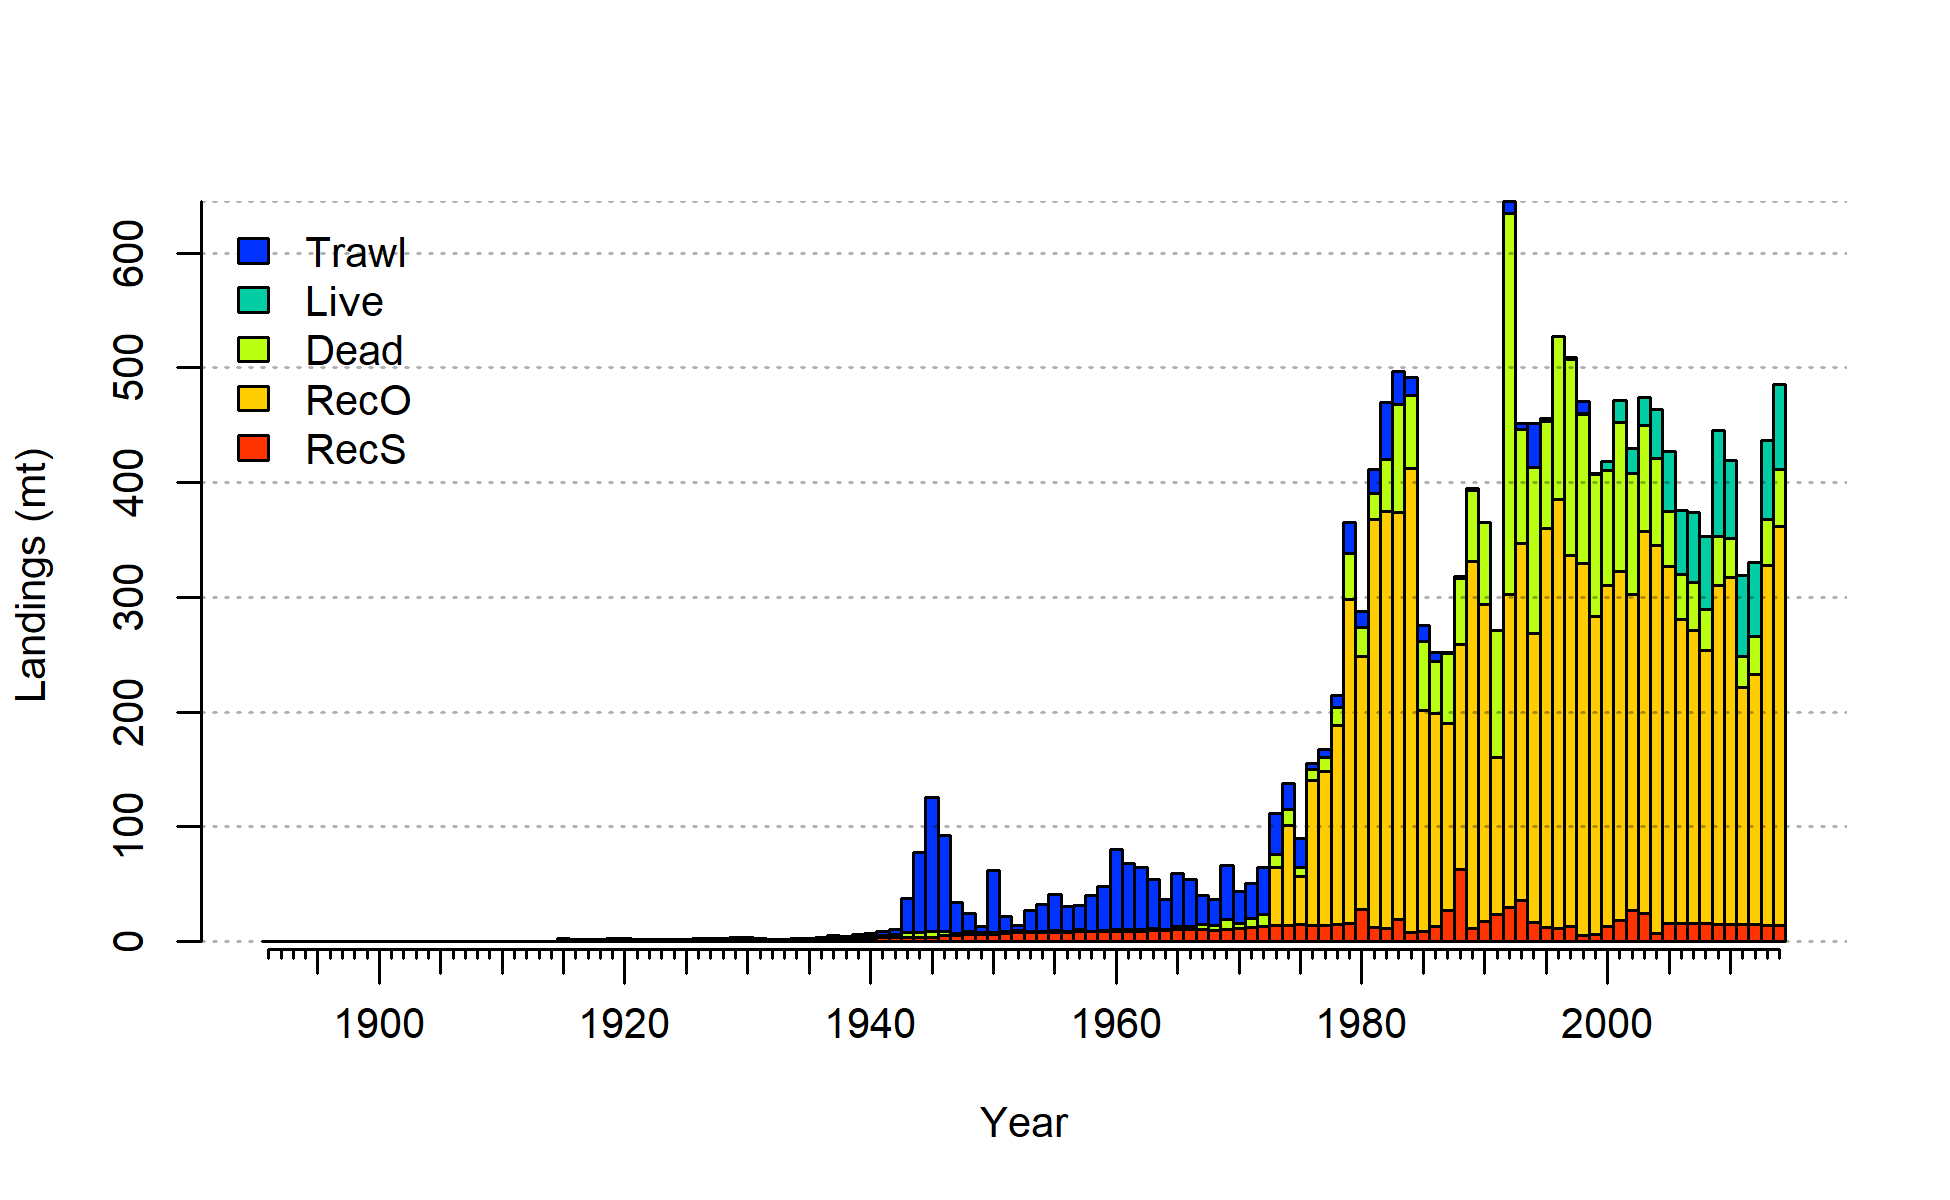
\includegraphics[width=1\textwidth,height=1\textheight]{C:/Users/Jason.Cope/Documents/Github/Sebastes_melanops_OR/Document/models/Reference model/plots/catch2 landings stacked.png}
\caption{Landings by fleet used in the reference model where catches in metric tons by fleet are stacked.\label{fig:es-catch}}
\end{figure}

\clearpage

\hypertarget{data-and-assessment}{%
\subsection*{Data and Assessment}\label{data-and-assessment}}
\addcontentsline{toc}{subsection}{Data and Assessment}

The first Black Rockfish stock assessment along the west coast of the United States that included the majority of Oregon waters was completed in 1993, covering the area south of Cape Falcon, Oregon to north of Point Piedros Blancos, California (Sampson 2007). Subsequent assesements that included Oregon waters were done in 2003 and 2007. In 2015, the last assessment prior to the current one was completed that included Oregon waters only as one of three (also Washington and California) seperate assessment areas delineated by state lines (Cope et al. 2016). Similarly, this assessment treats Oregon waters as a single assessment area. The previous two assessments used Stock Synthesis software, as does this one (version 3.30.21.00).

This assessment integrates data and information from multiple sources into one modeling framework. The stock assessment model for Black Rockfish is informed by catch data from two commercial fleets and two recreational fleets, six abundance indices, five sets of length composition data, and three sets of conditional age-at-length compositions. It also uses multiple ageing error matrices to incorporate ageing imprecision and applies fixed parameterizations of weight-at-length, maturity-at-length, fecundity-at-length, the Beverton-Holt stock-recruitment steepness value, and recruitment variability. Life history parameters were sex-specific (i.e., a two-sex model) with natural mortality fixed at external estimates and growth and recruitment parameters estimated. Additional parameters that were estimated include initial population scale (\(lnR_0\)), selectivity for each fishery and survey, and extra survey variance. The base model was tuned to account for the weighting of the length and age data and index variances (which was estimated), as well as the specification of the recruitment bias adjustments. Derived quantities include, among other things, the time series of spawning output, age and size structure, and current and projected future stock status. The model covers the years 1892 to 2022, with a 12 year forecast beginning in 2023.

Within model uncertainty is explicitly included in this assessment by parameter estimation uncertainty, while among model uncertainty is explored through sensitivity analyses addressing alternative input assumptions such as data treatment and weighting, and model specification sensitivity to the treatment of life history parameters, selectivity, recruitment, and survey catchability. A reference model was selected that best fit the observed data while concomitantly balancing the desire to capture the central tendency across those sources of uncertainty, ensure model realism and tractability, and promote robustness to potential model misspecification.

\hypertarget{stock-biomass-and-dynamics}{%
\subsection*{Stock Biomass and Dynamics}\label{stock-biomass-and-dynamics}}
\addcontentsline{toc}{subsection}{Stock Biomass and Dynamics}

Spawning output (in millions of eggs; meggs) instead of spawning biomass is used to report the functionally mature population scale because fecundity is nonlinearly related to body female weight. The estimated spawning output at the beginning of 2023 was 900 meggs (\textasciitilde95 percent asymptotic intervals: 855 to 944 meggs, Table \ref{tab:ssbES} and Figure \ref{fig:es-ssb}), which when compared to unfished spawning output (1,633 meggs) gives a relative stock status level of 55 percent (\textasciitilde95 percent asymptotic intervals: 53 to 57 percent, Figure \ref{fig:es-depl}). Overall, spawning output declined with the onset of increasing commercial removals in the 1960s and continued to decline with the increase in recreational catches through the 1990s, even dropping below the target relative stock size from 1993 to 2008, before steadily increasing back above target since that time. The largest of the estimated recruitment pulses occurred in 2008 and was followed by several above average recruitment years in the early 2010s, which contributed to the increase in spawning output through the mid to late 2010s. The minimum relative stock size of 25 percent of unfished levels is estimated to have occurred in 1999. Accordingly, the stock has not been below the minimum stock size threshold (i.e., never overfished based on median estimates). Currently the stock is estimated above the management target of \(SO_{40\%}\) in 2023 and is estimated to have remained above the target since 2009 (Table \ref{tab:ssbES} and Figure \ref{fig:es-depl}).

\begingroup\fontsize{10}{12}\selectfont
\begingroup\fontsize{10}{12}\selectfont

\begin{longtable}[t]{r>{\centering\arraybackslash}p{1.57cm}>{\centering\arraybackslash}p{1.57cm}>{\centering\arraybackslash}p{1.57cm}>{\centering\arraybackslash}p{1.57cm}>{\centering\arraybackslash}p{1.57cm}>{\centering\arraybackslash}p{1.57cm}}
\caption{\label{tab:ssbES}Estimated recent trend in spawning output and the fraction unfished and the 95 percent intervals.}\\
\toprule
Year & Spawning Output & Lower Interval & Upper Interval & Fraction Unfished & Lower Interval & Upper Interval\\
\midrule
\endfirsthead
\caption[]{Estimated recent trend in spawning output and the fraction unfished and the 95 percent intervals. \textit{(continued)}}\\
\toprule
Year & Spawning Output & Lower Interval & Upper Interval & Fraction Unfished & Lower Interval & Upper Interval\\
\midrule
\endhead

\endfoot
\bottomrule
\endlastfoot
2005 & 810.95 & 788.57 & 833.33 & 0.59 & 0.58 & 0.60\\
2006 & 807.26 & 784.84 & 829.68 & 0.59 & 0.58 & 0.59\\
2007 & 808.45 & 785.98 & 830.91 & 0.59 & 0.58 & 0.59\\
2008 & 810.93 & 788.42 & 833.44 & 0.59 & 0.58 & 0.60\\
2009 & 816.26 & 793.70 & 838.81 & 0.59 & 0.59 & 0.60\\
2010 & 813.90 & 791.32 & 836.49 & 0.59 & 0.58 & 0.60\\
2011 & 814.31 & 791.69 & 836.94 & 0.59 & 0.58 & 0.60\\
2012 & 822.04 & 799.37 & 844.72 & 0.60 & 0.59 & 0.60\\
2013 & 829.99 & 807.28 & 852.70 & 0.60 & 0.60 & 0.61\\
2014 & 829.72 & 806.98 & 852.46 & 0.60 & 0.60 & 0.61\\
2015 & 823.86 & 801.10 & 846.63 & 0.60 & 0.59 & 0.61\\*
\end{longtable}
\endgroup{}
\endgroup{}


\begin{figure}
\centering
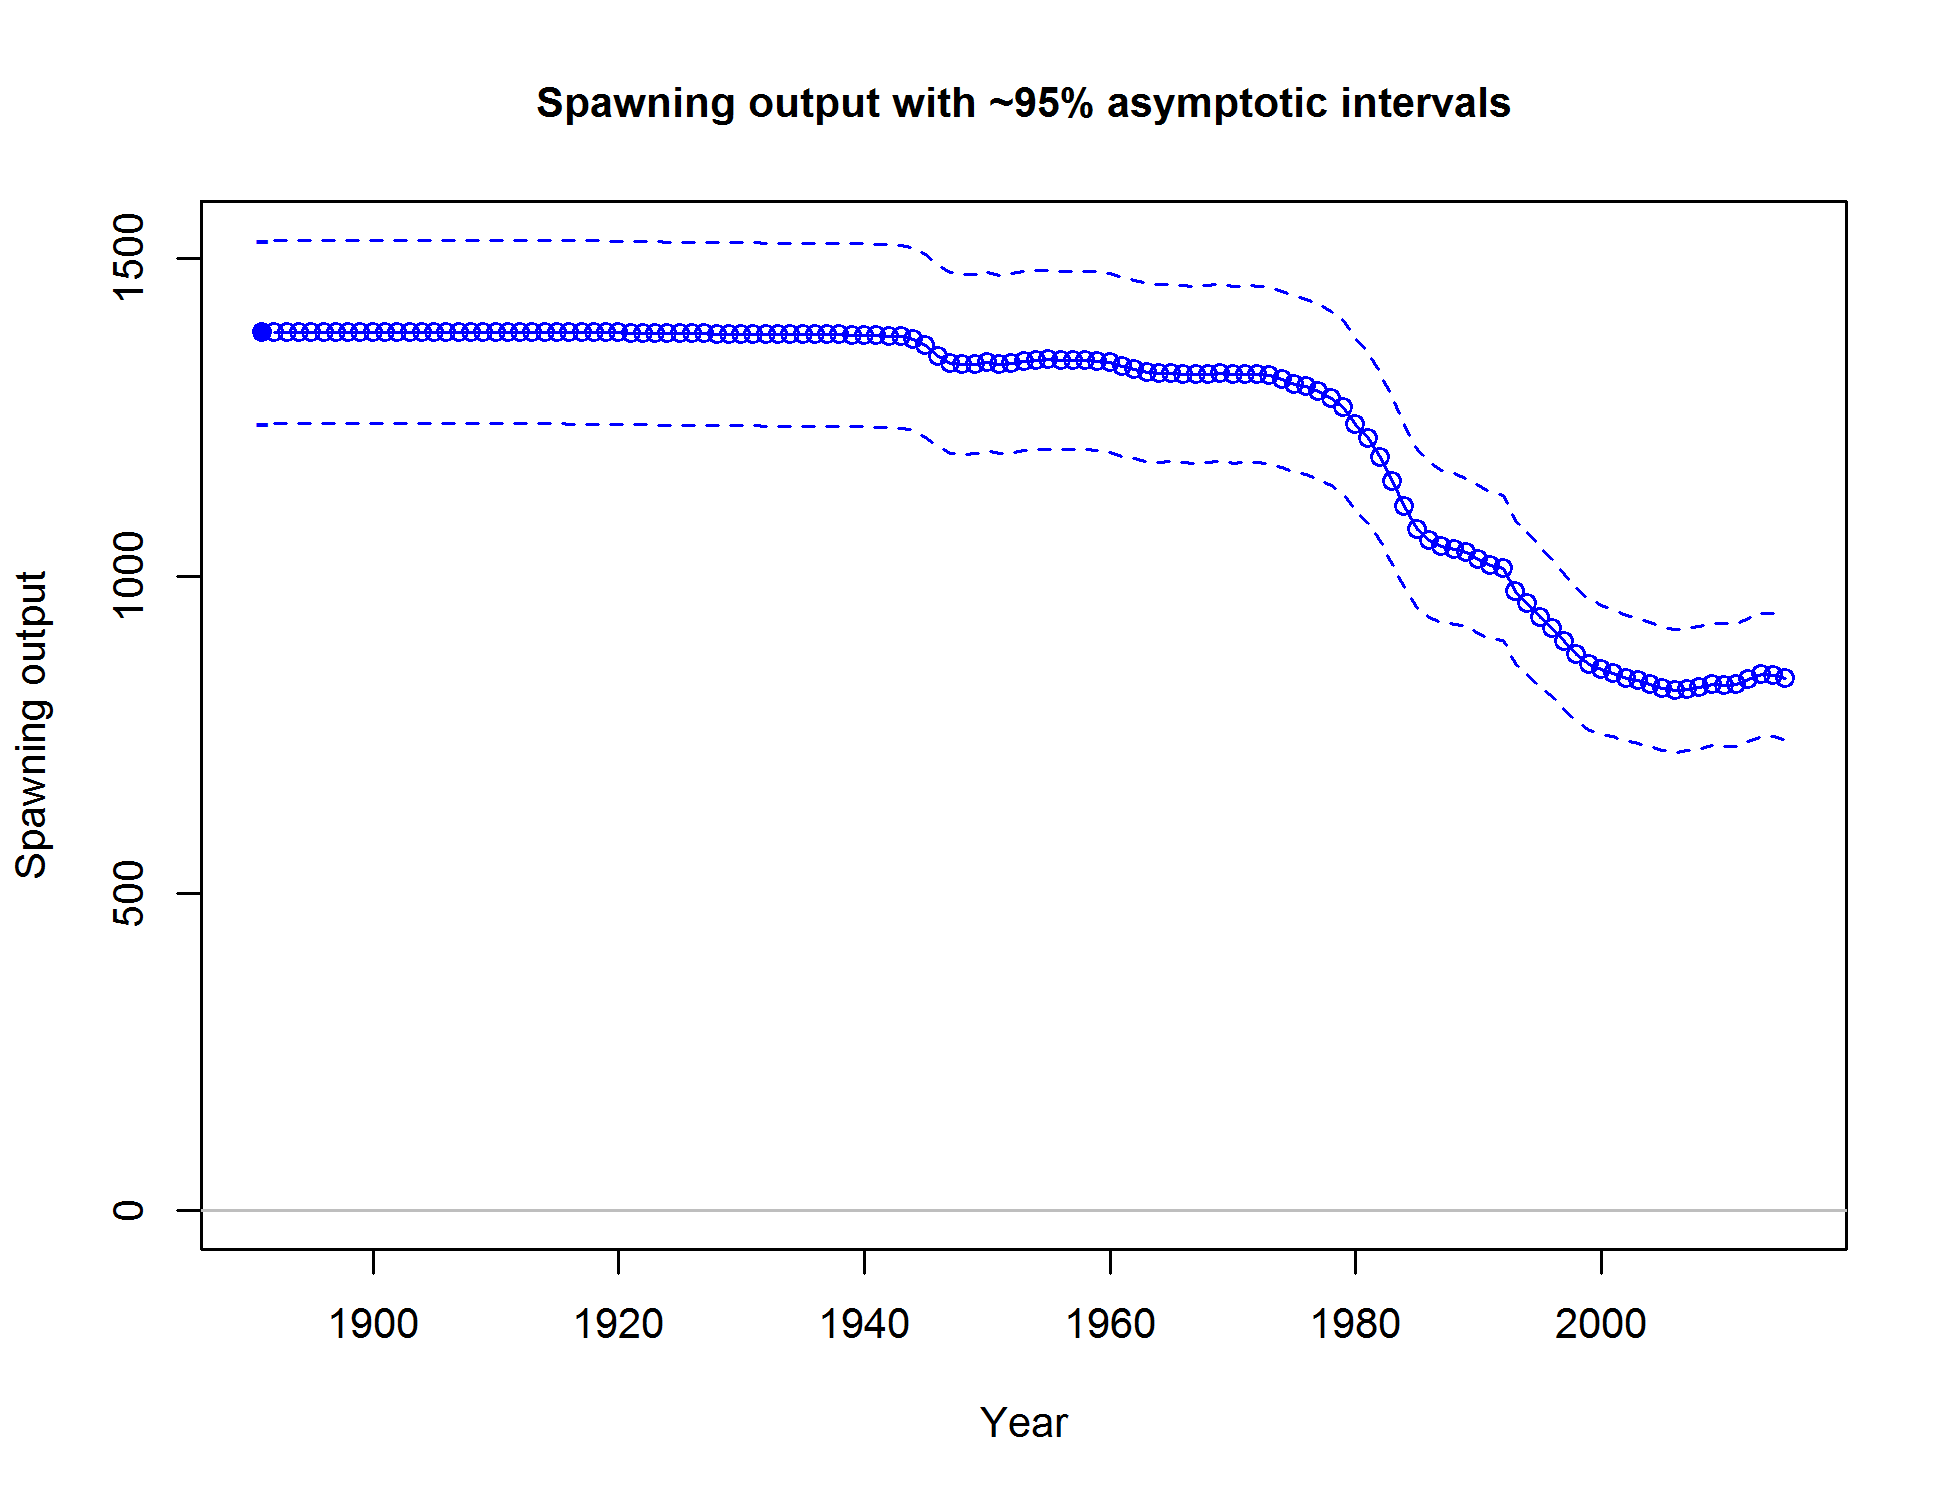
\includegraphics[width=1\textwidth,height=1\textheight]{C:/Users/Jason.Cope/Documents/Github/Sebastes_melanops_OR/Document/models/Reference model/plots/ts7_Spawning_output_with_95_asymptotic_intervals_intervals.png}
\caption{Estimated time series of spawning output (circles and line: median; light broken lines: 95 percent intervals) for the base model.\label{fig:es-ssb}}
\end{figure}

\begin{figure}
\centering
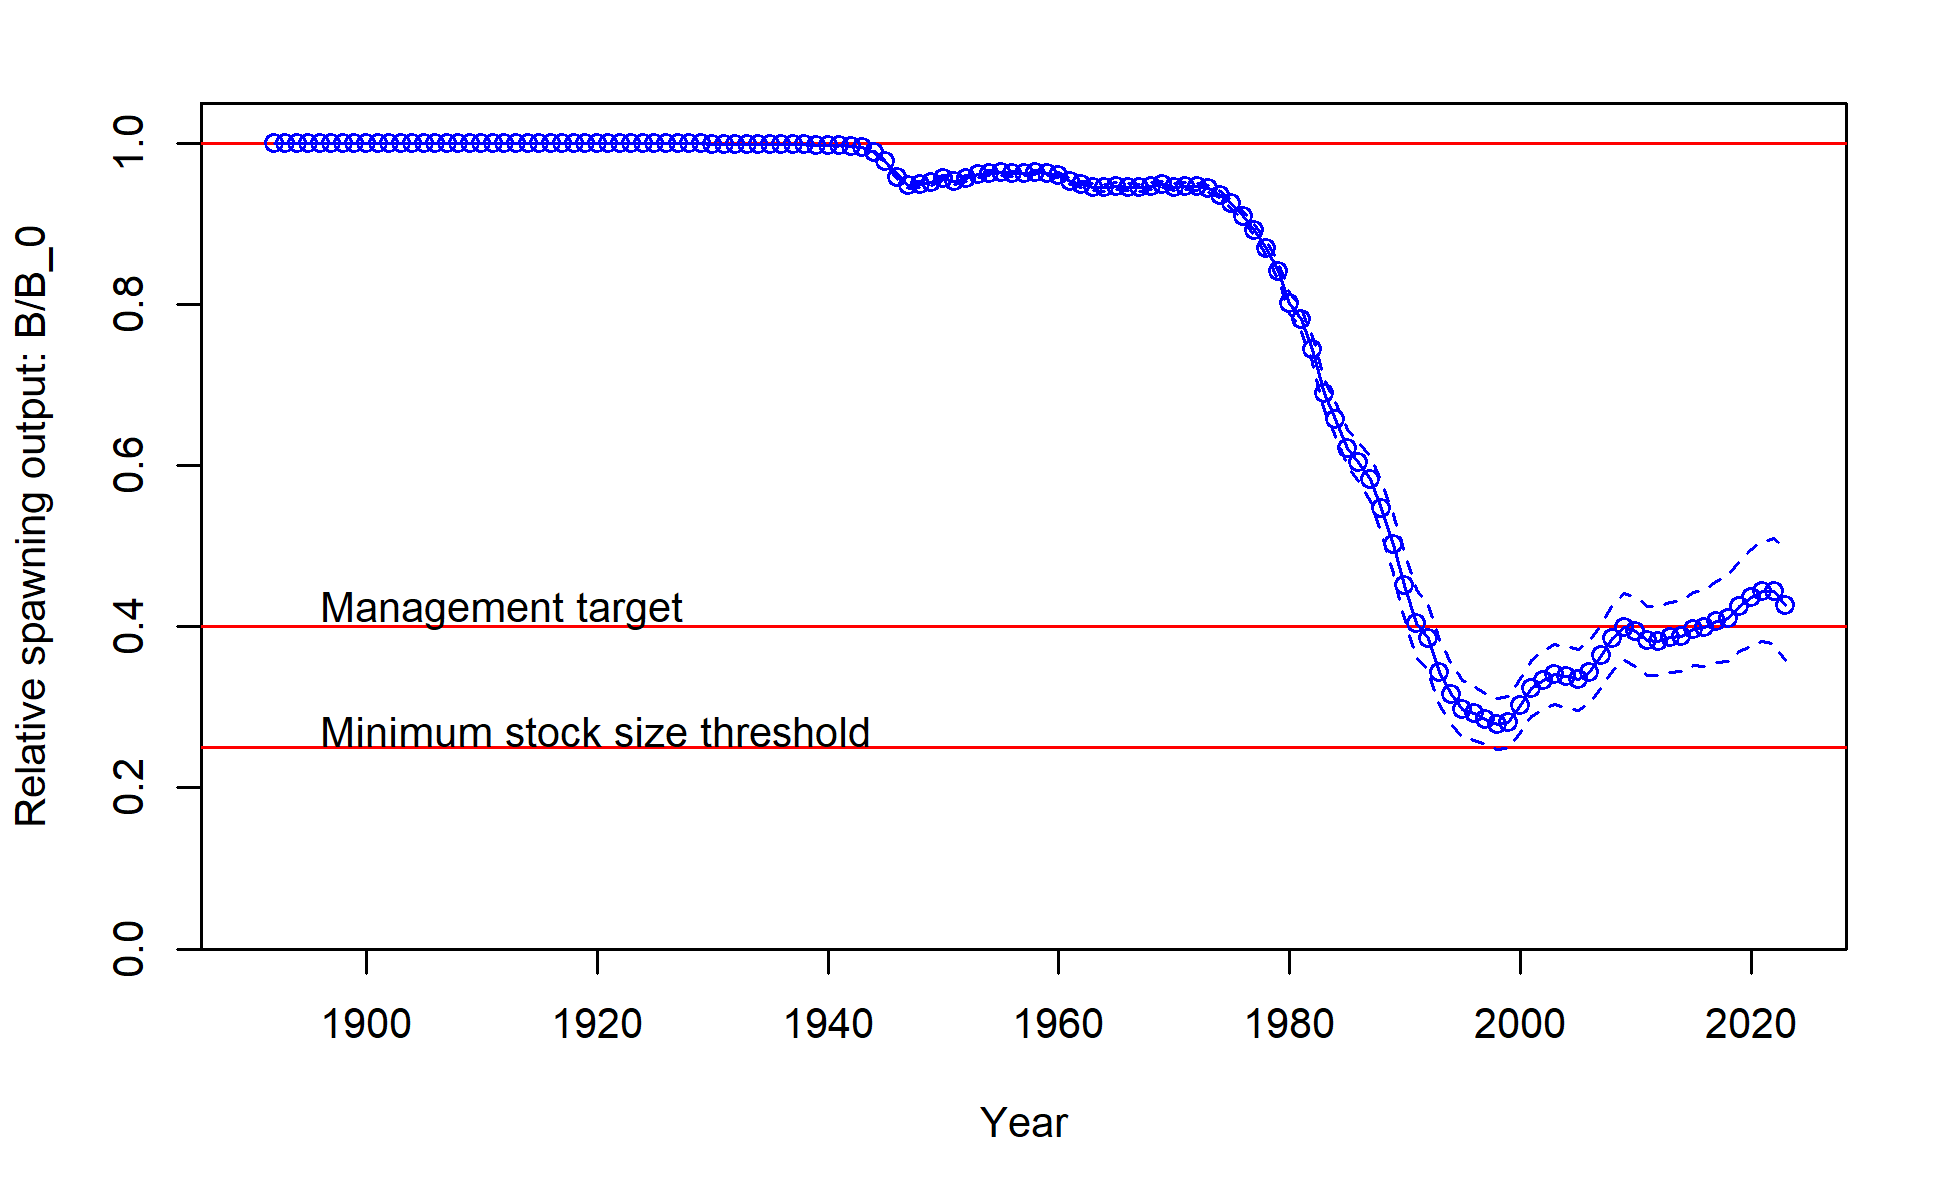
\includegraphics[width=1\textwidth,height=1\textheight]{C:/Users/Jason.Cope/Documents/Github/Sebastes_melanops_OR/Document/models/Reference model/plots/ts9_Relative_spawning_output_intervals.png}
\caption{Estimated time series of fraction of unfished spawning output (circles and line: median; light broken lines: 95 percent intervals) for the base model.\label{fig:es-depl}}
\end{figure}

\clearpage

\hypertarget{recruitment}{%
\subsection*{Recruitment}\label{recruitment}}
\addcontentsline{toc}{subsection}{Recruitment}

Recruitment is informed by the data and estimated from 1980 to 2017, before and after which it is assumed taken from the stock-recruit relationship (Table \ref{tab:recrES} and Figure \ref{fig:es-recruits}). The highest recruitment years occurred in 1999, 2000, 2008, 2013, and 2016. The large 2008 and 2016 year classes, as well as several above average year classes in the early 2010s, contributed to the recent increase in Black Rockfish biomass. Recruitment is informed by composition data and six relative abundance indices. The 2015 stock assessment did not estimate deviations from the stock-recruitment curve. While the Black Rockfish stock has been reduced to levels that theoretically would provide some information on how recruitment compensation changes across spawning output levels (i.e., inform the steepness parameter), the assessment model could not adequately estimate a reasonable steepness parameter. Thus, recruitment is based on a fixed assumption about steepness (\(h\) = 0.72) and recruitment variability (\(\sigma_R\) = 0.6).

\begingroup\fontsize{10}{12}\selectfont
\begingroup\fontsize{10}{12}\selectfont

\begin{longtable}[t]{r>{\centering\arraybackslash}p{2.2cm}>{\centering\arraybackslash}p{2.2cm}>{\centering\arraybackslash}p{2.2cm}>{\centering\arraybackslash}p{2.2cm}}
\caption{\label{tab:recrES}Estimated recent trend in recruitment (1,000s) and recruitment deviations and the 95 percent intervals for the model area.}\\
\toprule
Year & Recruitment (1,000s) & Interval & Recruitment Deviations & Interval\\
\midrule
\endfirsthead
\caption[]{Estimated recent trend in recruitment (1,000s) and recruitment deviations and the 95 percent intervals for the model area. \textit{(continued)}}\\
\toprule
Year & Recruitment (1,000s) & Interval & Recruitment Deviations & Interval\\
\midrule
\endhead

\endfoot
\bottomrule
\endlastfoot
2013 & 3,895 & 3,283–4,620 & 0.47 & 0.326–0.614\\
2014 & 3,481 & 2,880–4,207 & 0.36 & 0.196–0.522\\
2015 & 1,587 & 1,197–2,106 & -0.43 & -0.692–-0.167\\
2016 & 3,886 & 3,079–4,904 & 0.47 & 0.259–0.673\\
2017 & 1,009 & 623–1,637 & -0.93 & -1.401–-0.456\\
2018 & 2,906 & 2,695–3,133 & 0.00 & 0.000–0.000\\
2019 & 2,928 & 2,715–3,158 & 0.00 & 0.000–0.000\\
2020 & 2,946 & 2,730–3,179 & 0.00 & 0.000–0.000\\
2021 & 2,958 & 2,739–3,195 & 0.00 & 0.000–0.000\\
2022 & 2,962 & 2,737–3,204 & 0.00 & 0.000–0.000\\
2023 & 2,942 & 2,709–3,195 & 0.00 & 0.000–0.000\\*
\end{longtable}
\endgroup{}
\endgroup{}


\begin{figure}
\centering
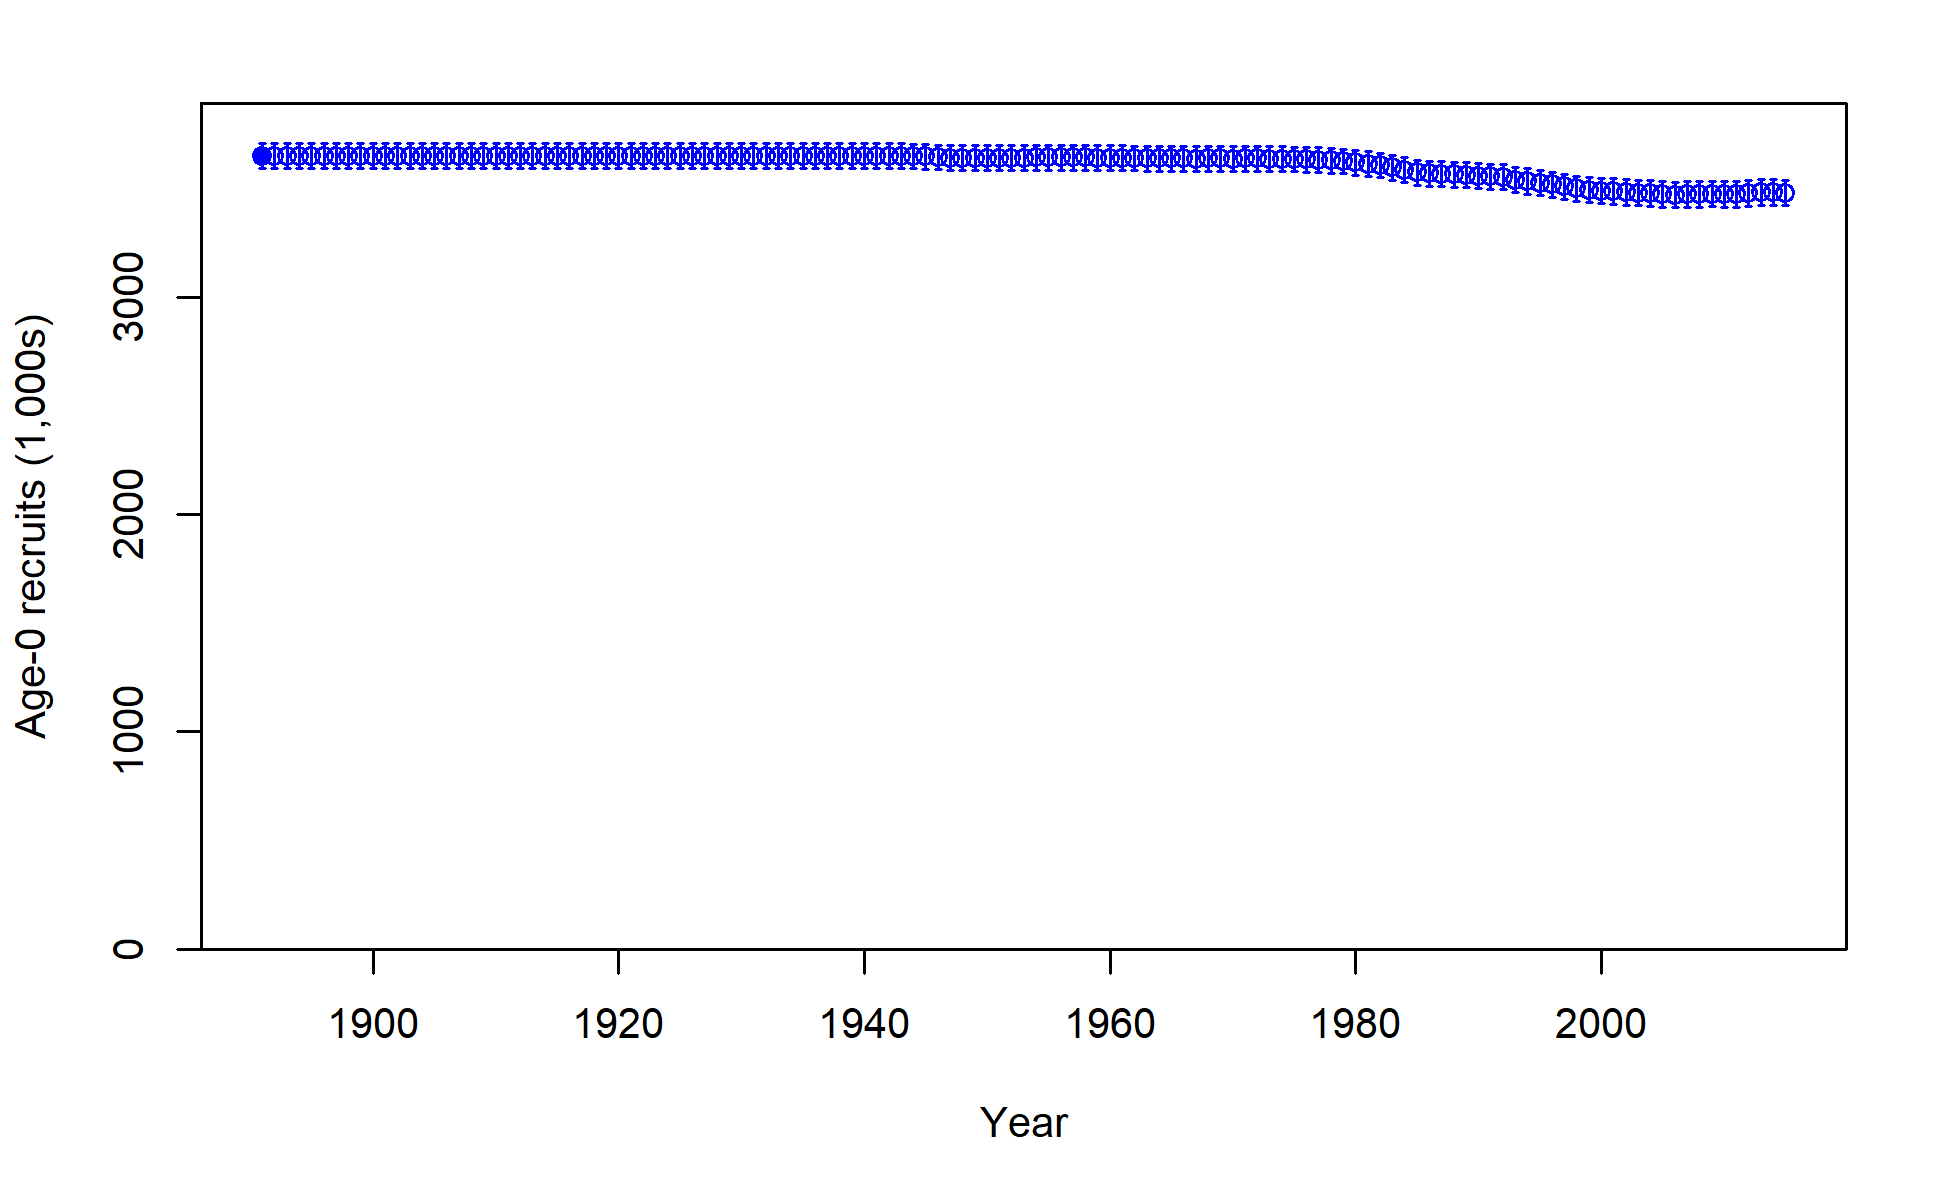
\includegraphics[width=1\textwidth,height=1\textheight]{C:/Users/Jason.Cope/Documents/Github/Sebastes_melanops_OR/Document/models/Reference model/plots/ts11_Age-0_recruits_(1000s)_with_95_asymptotic_intervals.png}
\caption{Estimated time series of age-0 recruits (1000s) for the base model with 95 percent intervals.\label{fig:es-recruits}}
\end{figure}

\begin{figure}
\centering
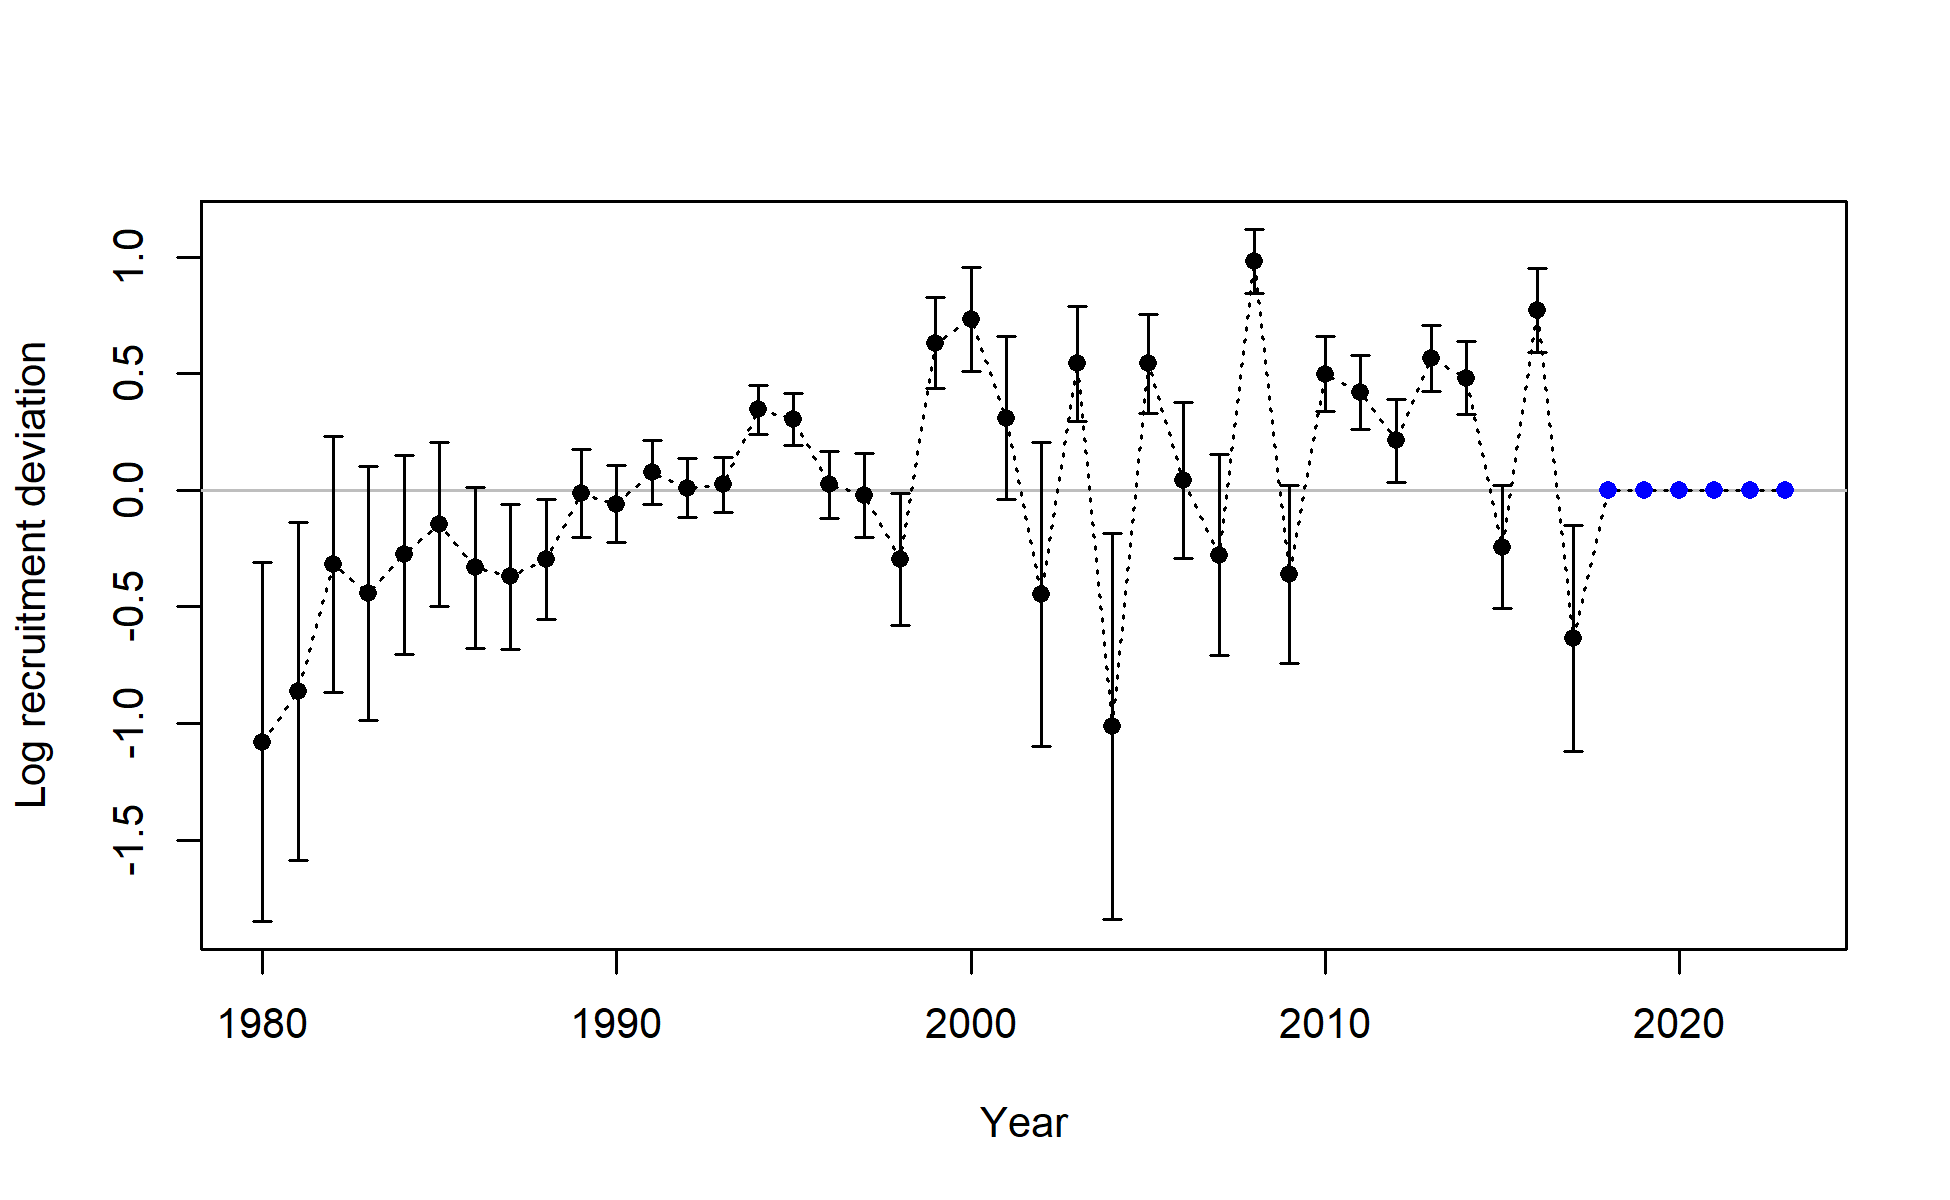
\includegraphics[width=1\textwidth,height=1\textheight]{C:/Users/Jason.Cope/Documents/Github/Sebastes_melanops_OR/Document/models/Reference model/plots/recdevs2_withbars.png}
\caption{Estimated time series of recruitment deviations.\label{fig:es-recdev}}
\end{figure}

\hypertarget{exploitation-status}\)) since 1980. Fishing was at or above the target rate from 1989 to 2005 and has been slightly below it over the past 5 years (Table \ref{tab:exploitES} and Figures \ref{fig:es-1-spr} and \ref{fig:es-phase}). The steepness value of 0.72 indicates that a lower value of SPR (or equivalently a higher fishing intensity than \(\text{SPR}_{50\%}\)) would be consistent with the spawning output-based target of (\(\text{SO}_{40\%}\)) for sustainable removals. Trends in fishing intensity largely mirrored that of landings until the 1990s, after which recruitment pulses countered the catches somewhat to lower overall fishing intensity (Figure \ref{fig:es-1-spr}). The maximum fishing intensity (1 - SPR) was 0.7 in 1992, which is well above the target of 0.50. The current level of 0.42 for 2022 is below that target. Fishing intensity over the past decade has ranged between 0.4 and 0.56 and the exploitation rate (range of 0.04 - 0.08, Table \ref{tab:exploitES}) has come down since the time series high of 0.12 in 1992. Current estimates indicate that Black Rockfish spawning output is greater than than the target biomass level (\(\text{SO}_{40\%}\)), though fishing intensity remains near the target \(F_{MSY}\) proxy harvest rate of 1 - \(\text{SPR}_{50\%}\) (Figure \ref{fig:es-phase}).

\begingroup\fontsize{10}{12}\selectfont
\begingroup\fontsize{10}{12}\selectfont

\begin{longtable}[t]{r>{\centering\arraybackslash}p{1.57cm}>{\centering\arraybackslash}p{1.57cm}>{\centering\arraybackslash}p{1.57cm}>{\centering\arraybackslash}p{1.57cm}>{\centering\arraybackslash}p{1.57cm}>{\centering\arraybackslash}p{1.57cm}}
\caption{\label{tab:exploitES}Estimated recent trend in the 1-SPR where SPR is the spawning potential ratio the exploitation rate, and the  95 percent intervals.}\\
\toprule
Year & 1-SPR & Lower Interval & Upper Interval & Exploitation Rate & Lower Interval & Upper Interval\\
\midrule
\endfirsthead
\caption[]{Estimated recent trend in the 1-SPR where SPR is the spawning potential ratio the exploitation rate, and the  95 percent intervals. \textit{(continued)}}\\
\toprule
Year & 1-SPR & Lower Interval & Upper Interval & Exploitation Rate & Lower Interval & Upper Interval\\
\midrule
\endhead

\endfoot
\bottomrule
\endlastfoot
2005 & 0.39 & 0.39 & 0.40 & 0.05 & 0.05 & 0.05\\
2006 & 0.36 & 0.35 & 0.36 & 0.05 & 0.05 & 0.05\\
2007 & 0.35 & 0.35 & 0.36 & 0.05 & 0.05 & 0.05\\
2008 & 0.34 & 0.33 & 0.34 & 0.04 & 0.04 & 0.04\\
2009 & 0.40 & 0.40 & 0.41 & 0.05 & 0.05 & 0.06\\
2010 & 0.38 & 0.38 & 0.39 & 0.05 & 0.05 & 0.05\\
2011 & 0.31 & 0.31 & 0.32 & 0.04 & 0.04 & 0.04\\
2012 & 0.32 & 0.31 & 0.32 & 0.04 & 0.04 & 0.04\\
2013 & 0.39 & 0.38 & 0.40 & 0.05 & 0.05 & 0.05\\
2014 & 0.42 & 0.42 & 0.43 & 0.06 & 0.06 & 0.06\\*
\end{longtable}
\endgroup{}
\endgroup{}


\begin{figure}
\centering
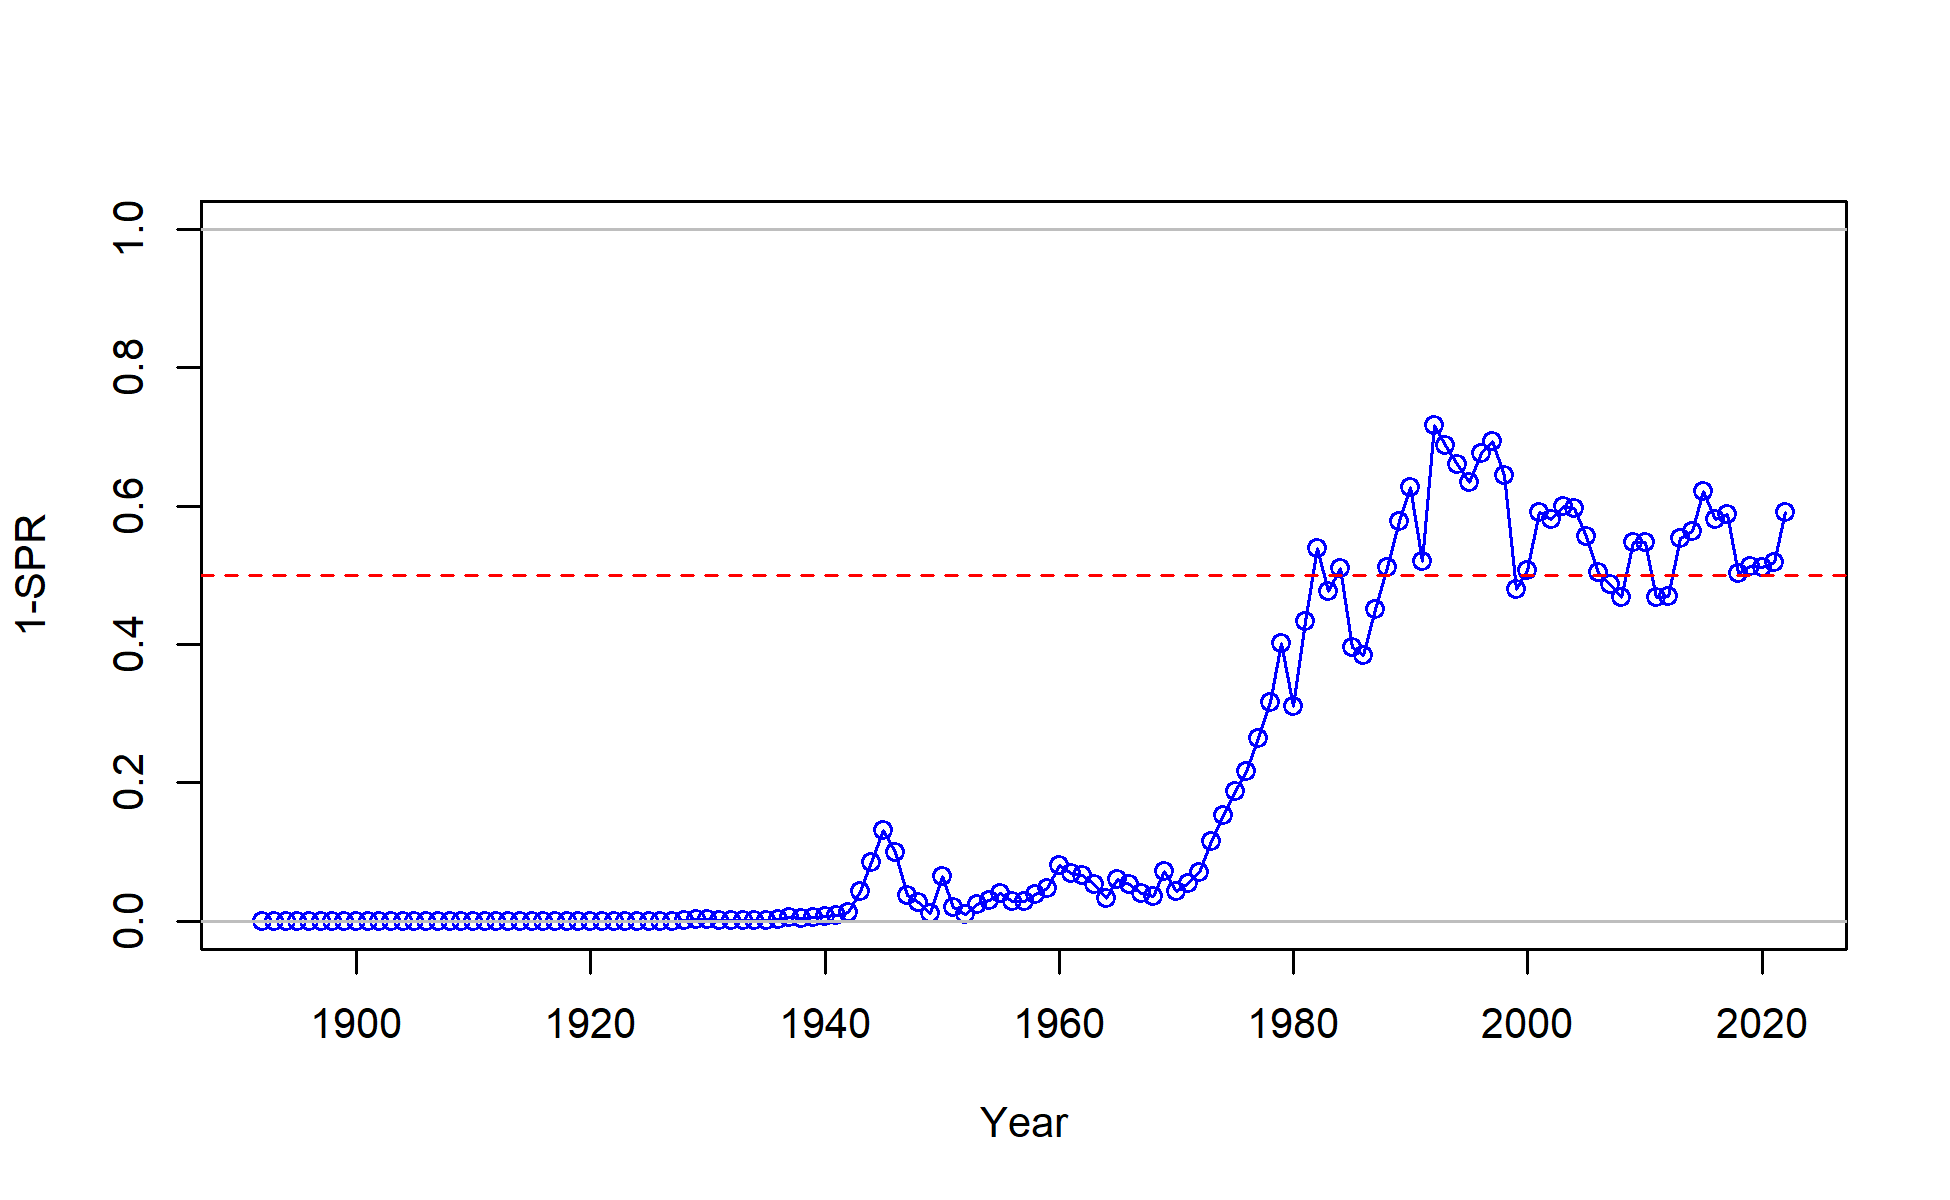
\includegraphics[width=1\textwidth,height=1\textheight]{C:/Users/Jason.Cope/Documents/Github/Sebastes_melanops_OR/Document/models/Reference model/plots/SPR2_minusSPRseries.png}
\caption{Estimated 1 - relative spawning ratio (SPR) by year for the base model. The management target is plotted as a red horizontal line and values above this reflect harvest in excess of the proxy harvest rate.\label{fig:es-1-spr}}
\end{figure}

\begin{figure}
\centering
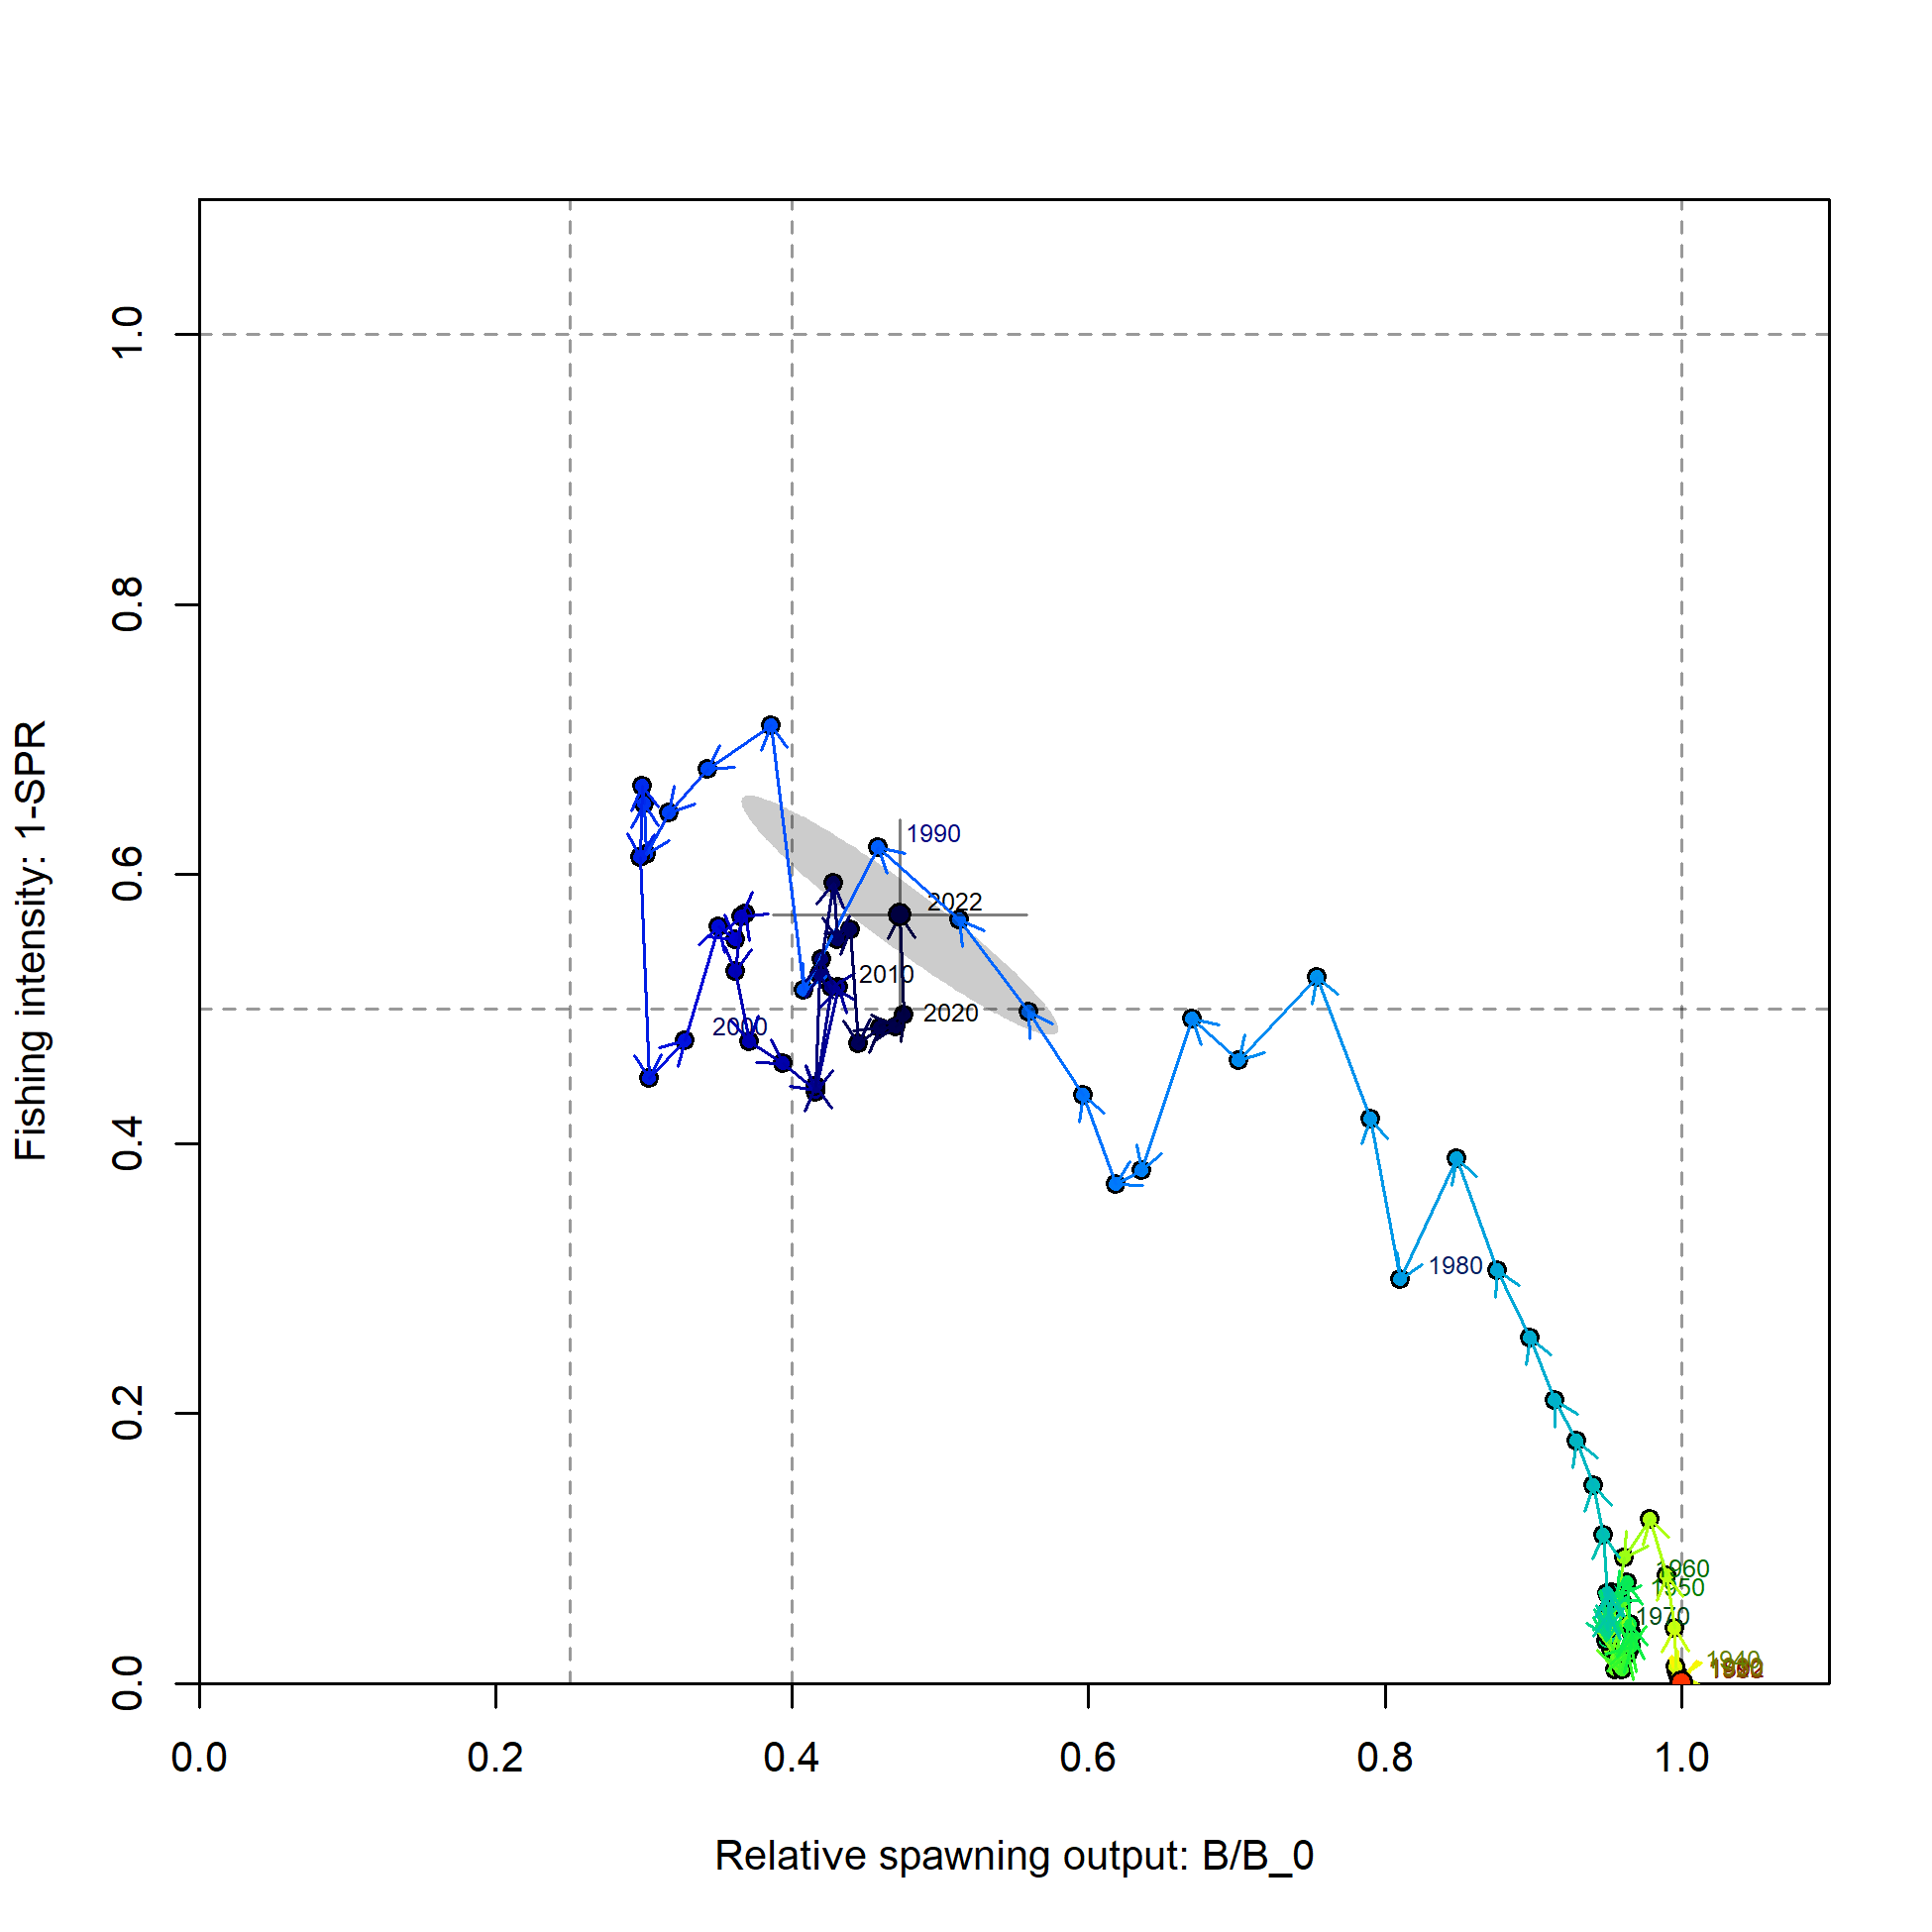
\includegraphics[width=1\textwidth,height=1\textheight]{C:/Users/Jason.Cope/Documents/Github/Sebastes_melanops_OR/Document/models/Reference model/plots/SPR4_phase.png}
\caption{Phase plot of estimated 1-SPR versus fraction unfished for the base model.\label{fig:es-phase}}
\end{figure}

\clearpage

\hypertarget{ecosystem-considerations}{%
\subsection*{Ecosystem Considerations}\label{ecosystem-considerations}}
\addcontentsline{toc}{subsection}{Ecosystem Considerations}

This stock assessment does not explicitly incorporate trophic interactions, habitat factors or environmental factors into the assessment model. More predation, diet and habitat work, and mechanistic linkages to environmental conditions would be needed to incorporate these elements into the stock assessment and should remain a priority. McClure et al. (2023) report the climate vulnerability for several west coast groundfishes, including Black Rockfish. Black Rockfish demonstrated both high biological sensitivity and high climate exposure risk, to give it an overall high vulnerability score to climate change. This result should also be considered with the fact that, like many rockfishes, periods of low productivity are not unusual to Black Rockfish and their extended longevity (though admittedly this seems shorter than previously believed and should be reconsidered) has historically allowed them to wait for advantageous productivity periods. Additional stressors such as fishing and climate change that possibly truncate longevity could bring significant challenges to population sustainability.

\hypertarget{reference-points}\)), target relative spawning output (40\%), and estimated selectivity and catch for each fleet (Table \ref{tab:referenceES}). The yield values are lower than the previous assessment for similar reference points due to updated life history estimates. The proxy FMSY values of management quantities, based on exploitation rates that achieve \(\text{SPR}_{50\%}\) and \(\text{SO}_{40\%}\), are more conservative (lower) than the exploitation rate at estimated MSY. Sustainable total yield using the proxy \(\text{SPR}_{50\%}\) is 455 mt. The spawning output equivalent to 40 percent of the unfished spawning output (\(\text{SO}_{40\%}\)) was 653.1 meggs.

Recent removals have been close to the point estimate of potential long-term yields calculated using an \(\text{SPR}_{50\%}\) reference point, though the population size has continued to increase over recent years due to several above average recruitments. The equilibrium estimates of yield relative to biomass based on a steepness value fixed at 0.72 are provided in Figure \ref{fig:es-yield}, where vertical dashed lines indicate the estimate of fraction unfished at the start of 2023 (current) and the estimated management targets calculated based on the relative target biomass (B target), the SPR target, and the maximum sustainable yield (MSY).

The 2023 spawning output relative to unfished equilibrium spawning output is above (55 percent) the management target of 40 percent of unfished spawning output (i.e., 1.38 times above the target spawning output; Figure \ref{fig:es-phase}). The relative biomass and the ratio of the estimated SPR to the management target (\(\text{SPR}_{50\%}\)) across all model years are shown in Figure \ref{fig:es-phase} where warmer colors (red) represent early years and colder colors (blue) represent recent years. There have been periods where the stock status has decreased below the target and fishing intensity has been higher than the target fishing intensity based on \(\text{SPR}_{50\%}\). Fishing intensity during the most recent year (2022) is estimated to be slightly below the fishing intensity target (0.96 times \(\text{SPR}_{50\%}\); Figure \ref{fig:es-phase}).

\begin{figure}
\centering
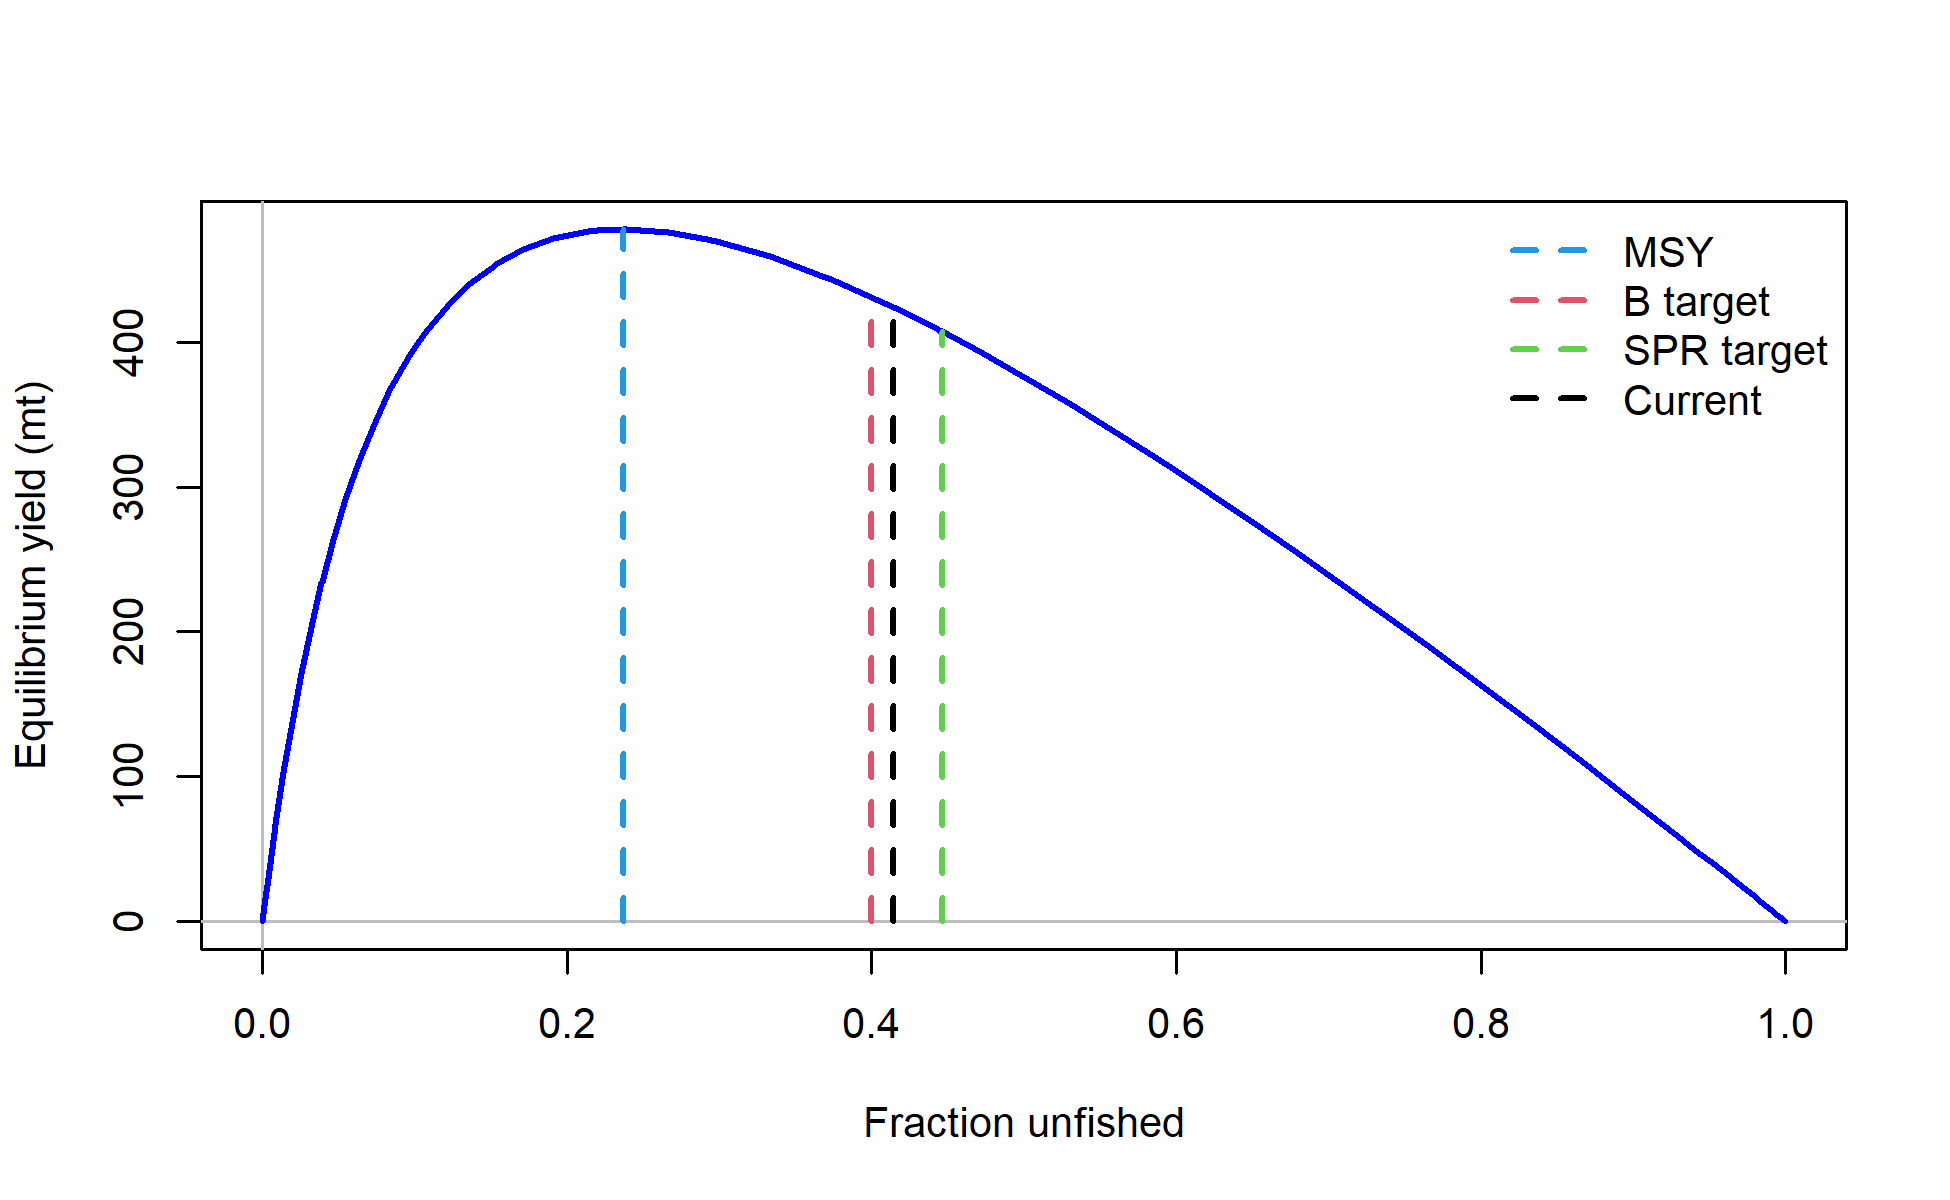
\includegraphics[width=1\textwidth,height=1\textheight]{C:/Users/Jason.Cope/Documents/Github/Sebastes_melanops_OR/Document/models/Reference model/plots/yield2_yield_curve_with_refpoints.png}
\caption{Equilibrium yield curve for the base case model. Values are based on (the time invariant) fishery selectivities and with steepness fixed at 0.72.\label{fig:es-yield}}
\end{figure}

\clearpage

\begingroup\fontsize{10}{12}\selectfont
\begingroup\fontsize{10}{12}\selectfont

\begin{longtable}[t]{r>{\centering\arraybackslash}p{2cm}>{\centering\arraybackslash}p{2cm}>{\centering\arraybackslash}p{2cm}}
\caption{\label{tab:referenceES}Summary of reference points and management quantities, including median estimates and associated 95 percent intervals.}\\
\toprule
 & Estimate & Lower Interval & Upper Interval\\
\midrule
\endfirsthead
\caption[]{Summary of reference points and management quantities, including median estimates and associated 95 percent intervals. \textit{(continued)}}\\
\toprule
 & Estimate & Lower Interval & Upper Interval\\
\midrule
\endhead

\endfoot
\bottomrule
\endlastfoot
Unfished Spawning Output & 1632.81 & 1577.19 & 1688.43\\
Unfished Age 0+ Biomass (mt) & 11576.10 & 11142.20 & 12010.00\\
Unfished Recruitment (R0) & 3807.86 & 3678.16 & 3937.56\\
Spawning Output (2023) & 899.77 & 855.05 & 944.49\\
Fraction Unfished (2023) & 0.55 & 0.53 & 0.57\\
Reference Points Based SB40\textbackslash{}\% & - & - & -\\
Proxy Spawning Output SB40\textbackslash{}\% & 653.12 & 630.88 & 675.37\\
SPR Resulting in SB40\textbackslash{}\% & 0.46 & 0.46 & 0.46\\
Exploitation Rate Resulting in SB40\textbackslash{}\% & 0.07 & 0.07 & 0.07\\
Yield with SPR Based On SB40\textbackslash{}\% (mt) & 481.51 & 464.00 & 499.03\\
Reference Points Based on SPR Proxy for MSY & - & - & -\\
Proxy Spawning Output (SPR50) & 728.48 & 703.67 & 753.30\\
SPR50 & 0.50 &   &  \\
Exploitation Rate Corresponding to SPR50 & 0.06 & 0.06 & 0.07\\
Yield with SPR50 at SB SPR (mt) & 454.96 & 438.30 & 471.63\\
Reference Points Based on Estimated MSY Values & - & - & -\\
Spawning Output at MSY (SB MSY) & 386.95 & 373.08 & 400.83\\
SPR MSY & 0.31 & 0.31 & 0.31\\
Exploitation Rate Corresponding to SPR MSY & 0.11 & 0.11 & 0.11\\
MSY (mt) & 533.65 & 514.71 & 552.60\\*
\end{longtable}
\endgroup{}
\endgroup{}


\clearpage

\hypertarget{management-performance}{%
\subsection*{Management Performance}\label{management-performance}}
\addcontentsline{toc}{subsection}{Management Performance}

Black Rockfish removals have generally been below the equivalent ABC-ACL over the recent decade, with the exception of 2017 and 2022 when removals were slightly higher (Table \ref{tab:manageES}). Exploitation on Black Rockfish increased starting around 1940 and reached a high in the late 1970s. Since that time, catch has mostly fluctuated between 300 and 500 mt per year, with some years exceeding 600 mt. Removals have averaged 483 mt over the past decade. The last ten years of Black Rockfish acceptable biological catch (ABC) and annual catch limit (ACL) have been set, by definition, below the overfishing limit (OFL) (Table \ref{tab:manageES}). Prior to 2017, management specifications were set for Black Rockfish in California and Oregon waters combined. The Black Rockfish OFL has not been exceeded by Oregon removals over the past decade. The ACL and ABC were exceeded in 2017 and 2022 by a small margin, but were more than offset by underages in intervening years.

\begingroup\fontsize{10}{12}\selectfont
\begingroup\fontsize{10}{12}\selectfont

\begin{longtable}[t]{r>{\centering\arraybackslash}p{2.2cm}>{\centering\arraybackslash}p{2.2cm}>{\centering\arraybackslash}p{2.2cm}>{\centering\arraybackslash}p{2.2cm}}
\caption{\label{tab:manageES}Recent trend in the overfishing limits (OFL), the acceptable biological catches (ABCs),
                the annual catch limits (ACLs), and the total catch (mt).}\\
\toprule
Year & OFL & ABC & ACL & Catch\\
\midrule
\endfirsthead
\caption[]{Recent trend in the overfishing limits (OFL), the acceptable biological catches (ABC \textit{(continued)}}\\
\toprule
Year & OFL & ABC & ACL & Catch\\
\midrule
\endhead

\endfoot
\bottomrule
\endlastfoot
2005 & fill in & fill in & fill in & 427.37\\
2006 & fill in & fill in & fill in & 375.71\\
2007 & fill in & fill in & fill in & 374.19\\
2008 & fill in & fill in & fill in & 353.23\\
2009 & fill in & fill in & fill in & 445.71\\
2010 & fill in & fill in & fill in & 419.60\\
2011 & fill in & fill in & fill in & 319.46\\
2012 & fill in & fill in & fill in & 330.26\\
2013 & fill in & fill in & fill in & 436.29\\
2014 & fill in & fill in & fill in & 485.34\\*
\end{longtable}
\endgroup{}
\endgroup{}


\hypertarget{unresolved-problems-and-major-uncertainties}{%
\subsection*{Unresolved Problems and Major Uncertainties}\label{unresolved-problems-and-major-uncertainties}}
\addcontentsline{toc}{subsection}{Unresolved Problems and Major Uncertainties}

The biggest uncertainty and unresolved conflict is trying to reconcile the signal in the biological data (which suggests a lower population size and status) versus the acoustic and tag surveys (which suggest high stock sizes and status). This is the major issue the current assessment is confronting. Another acoustic-visual survey data point could help resolve how much uncertainty there is in the estimate. The lack of contrast in the biological data, despite large sample sizes, is another barrier to interpreting the current conditions, though given models using only biological data, the signal seems clear that the population could be at a lower stock status.

\hypertarget{scientific-uncertainty}{%
\subsection*{Scientific Uncertainty}\label{scientific-uncertainty}}
\addcontentsline{toc}{subsection}{Scientific Uncertainty}

The model-estimated uncertainty around the 2023 spawning output was \(\sigma\) = 0.03 and the uncertainty around the OFL was \(\sigma\) = 0.01. This is clearly an underestimate of overall uncertainty because of the necessity to fix some life history parameters such as natural mortality and steepness, as well as a lack of explicit incorporation of model structural uncertainty. The alternative states of nature used to bracket uncertainty in the decision table assist with encapsulating model structure uncertainty.

\hypertarget{harvest-projections-and-decision-table}{%
\subsection*{Harvest Projections and Decision Table}\label{harvest-projections-and-decision-table}}
\addcontentsline{toc}{subsection}{Harvest Projections and Decision Table}

The following text will be modified, as appropriate, after the STAR panel and SSC meeting.

The Black Rockfish assessment is being considered as a category 2 assessment with a \(P^*\) = 0.45, sigma = 0.72, and a time-varying buffer applied to the OFL. These multipliers are also combined with the rockfish MSY proxy of FSPR=50\% MSY and the 40-10 harvest control rule to calculate OFLs, ABCs and ACLs. A twelve year (2023-2034) projection of the reference model using these specifications along with input removals for 2023 and 2024 provided by the Groundfish Management Team is provided in Table \ref{tab:projectionES}.

\begingroup\fontsize{10}{12}\selectfont
\begingroup\fontsize{10}{12}\selectfont

\begin{longtable}[t]{r>{\centering\arraybackslash}p{1.83cm}>{\centering\arraybackslash}p{1.83cm}>{\centering\arraybackslash}p{1.83cm}>{\centering\arraybackslash}p{1.83cm}>{\centering\arraybackslash}p{1.83cm}}
\caption{\label{tab:projectionES}Projections of potential OFLs (mt), ABCs (mt), estimated spawning output, and fraction unfished.}\\
\toprule
Year & Predicted OFL (mt) & ABC Catch (mt) & Age 0+ Biomass (mt) & Spawning Output & Fraction Unfished\\
\midrule
\endfirsthead
\caption[]{Projections of potential OFLs (mt), ABCs (mt), estimated spawning output, and fraction unfished. \textit{(continued)}}\\
\toprule
Year & Predicted OFL (mt) & ABC Catch (mt) & Age 0+ Biomass (mt) & Spawning Output & Fraction Unfished\\
\midrule
\endhead

\endfoot
\bottomrule
\endlastfoot
2023	&	541.9	&	496.5	&	1.00	&	7981.8	 &	899.8	&	0.55\\
2024	&	-	&	-	&	-	&	-	 &	-	&	-\\
2025	&	-	&	-	&	-	&	-	 &	-	&	-\\
2026	&	-	&	-	&	-	&	-	 &	-	&	-\\
2027	&	-	&	-	&	-	&	-	 &	-	&	-\\
2028	&	-	&	-	&	-	&	-	 &	-	&	-\\
2029	&	-	&	-	&	-	&	-	 &	-	&	-\\
2030	&	-	&	-	&	-	&	-	 &	-	&	-\\
2031	&	-	&	-	&	-	&	-	 &	-	&	-\\
2032	&	-	&	-	&	-	&	-	 &	-	&	-\\
2033	&	-	&	-	&	-	&	-	 &	-	&	-\\
2034	&	-	&	-	&	-	&	-	 &	-	&	-\\*
\end{longtable}
\endgroup{}
\endgroup{}


Uncertainty in management quantities for the reference model was characterized by exploring various model specifications in a decision table. Initial explorations considered alternative specifications of catchability for the acoustic-visual survey. The resultant decision table will be provided in Table \ref{tab:es-dec-tab}.

Further details about selecting the decision table states of nature will be added here after the STAR panel.

\clearpage

\begingroup\fontsize{9}{11}\selectfont
\begingroup\fontsize{9}{11}\selectfont

\begin{longtable}[t]{l>{\raggedright\arraybackslash}p{0.08\linewidth}>{\raggedright\arraybackslash}p{0.08\linewidth}>{\raggedright\arraybackslash}p{0.1\linewidth}>{\raggedright\arraybackslash}p{0.09\linewidth}>{\raggedright\arraybackslash}p{0.1\linewidth}>{\raggedright\arraybackslash}p{0.09\linewidth}>{\raggedright\arraybackslash}p{0.1\linewidth}>{\raggedright\arraybackslash}p{0.09\linewidth}}
\caption{\label{tab:es-dec-tab}Decision table summary of 10 year projections beginning in 2023 for alternative states of nature based on an axis of uncertainty related to model structure relative to the reference model (i.e., estimate catchability, Q, associated with the acoustic-visual survey and no estimation of recruitment deviations) . Columns range over low (12.5 quantile), mid (reference model), and high states (87.5 quantile) of nature and rows range over different catch level assumptions. Values in italics indicate years where the stock size prevented the full catch removals.}\\
\toprule
\multicolumn{3}{c}{ } & \multicolumn{2}c{Estimate Q} & \multicolumn{2}c{Reference Model} & \multicolumn{2}c{No Rec Devs} \\
\cmidrule(l{3pt}r{3pt}){4-5} \cmidrule(l{3pt}r{3pt}){6-7} \cmidrule(l{3pt}r{3pt}){8-9}
  & Year & Catch & Spawning Output & Fraction Unfished & Spawning Output & Fraction Unfished & Spawning Output & Fraction Unfished\\
\hline
	&	2023	&	-	&	 - 	&	-	&	 - 	&	-	&	 - 	&	-\\	
	&	2024	&	-	&	 - 	&	-	&	 - 	&	-	&	 - 	&	-\\	
	&	2025	&	-	&	 - 	&	-	&	 - 	&	-	&	 - 	&	-\\
	&	2026	&	-	&	 - 	&	-	&	 - 	&	-	&	 - 	&	-\\
	&	2027	&	-	&	 - 	&	-	&	 - 	&	-	&	 - 	&	-\\
P*=0.45	&	2028	&	-	&	 - 	&	-	&	 - 	&	-	&	 - 	&	-\\
sigma=0.5	&	2029	&	-	&	 - 	&	-	&	 - 	&	-	&	 - 	&	-\\
	&	2030	&	-	&	 - 	&	-	&	 - 	&	-	&	 - 	&	-\\
	&	2031	&	-	&	 - 	&	-	&	 - 	&	-	&	 - 	&	-\\
	&	2032	&	-	&	 - 	&	-	&	 - 	&	-	&	 - 	&	-\\
	&	2033	&	-	&	 - 	&	-	&	 - 	&	-	&	 - 	&	-\\
	&	2034	&	-	&	 - 	&	-	&	 - 	&	-	&	 - 	&	-\\
\hline																
	&	2023	&	-	&	 - 	&	-	&	 - 	&	-	&	 - 	&	-\\
	&	2024	&	-	&	 - 	&	-	&	 - 	&	-	&	 - 	&	-\\
	&	2025	&	-	&	 - 	&	-	&	 - 	&	-	&	 - 	&	-\\
	&	2026	&	-	&	 - 	&	-	&	 - 	&	-	&	 - 	&	-\\
	&	2027	&	-	&	 - 	&	-	&	 - 	&	-	&	 - 	&	-\\
P*=0.4	&	2028	&	-	&	 - 	&	-	&	 - 	&	-	&	 - 	&	-\\
sigma=0.5	&	2029	&	-	&	 - 	&	-	&	 - 	&	-	&	 - 	&	-\\
	&	2030	&	-	&	 - 	&	-	&	 - 	&	-	&	 - 	&	-\\
	&	2031	&	-	&	 - 	&	-	&	 - 	&	-	&	 - 	&	-\\
	&	2032	&	-	&	 - 	&	-	&	 - 	&	-	&	 - 	&	-\\
	&	2033	&	-	&	 - 	&	-	&	 - 	&	-	&	 - 	&	-\\
	&	2034	&	-	&	 - 	&	-	&	 - 	&	-	&	 - 	&	-\\
\hline																
	&	2023	&	-	&	 - 	&	-	&	 - 	&	-	&	 - 	&	-\\
	&	2024	&	-	&	 - 	&	-	&	 - 	&	-	&	 - 	&	-\\
	&	2025	&	-	&	 - 	&	-	&	 - 	&	-	&	 - 	&	-\\
	&	2026	&	-	&	 - 	&	-	&	 - 	&	-	&	 - 	&	-\\
Equilibrium	&	2027	&	-	&	 - 	&	-	&	 - 	&	-	&	 - 	&	-\\
yield from	&	2028	&	-	&	 - 	&	-	&	 - 	&	-	&	 - 	&	-\\
FMSY proxy	&	2029	&	-	&	 - 	&	-	&	 - 	&	-	&	 - 	&	-\\
of SPR=0.5	&	2030	&	-	&	 - 	&	-	&	 - 	&	-	&	 - 	&	-\\
	&	2031	&	-	&	 - 	&	-	&	 - 	&	-	&	 - 	&	-\\
	&	2032	&	-	&	 - 	&	-	&	 - 	&	-	&	 - 	&	-\\
	&	2033	&	-	&	 - 	&	-	&	 - 	&	-	&	 - 	&	-\\
	&	2034	&	-	&	 - 	&	-	&	 - 	&	-	&	 - 	&	-\\*
\hline
\end{longtable}
\endgroup{}
\endgroup{}


\clearpage

\hypertarget{research-and-data-needs}{%
\subsection*{Research and Data Needs}\label{research-and-data-needs}}
\addcontentsline{toc}{subsection}{Research and Data Needs}

Recommended avenues for research to help improve future Black Rockfish stock assessments (in no particular order):

\begin{enumerate}
\def\labelenumi{\arabic{enumi}.}
\tightlist
\item
  Continue work on the investigation into the movement, and behavior or mortality of older (\textgreater{} age 10) females to further reconcile their absence in fisheries data.
\item
  Conduct population genetics studies on fish observed off of the continental shelf (middle of the gyre and at sea mounts) to determine their association with the nearshore stocks.
\item
  Continue to build evidence for appropriate natural mortality values for females and males.
\item
  Improved historical catch reconstructions. Specifically, the historic trawl fishery catches (pre-1987) in particular require particular attention. A synoptic catch reconstruction is recommended, where states work together to resolve cross-boundarystate catch issues as well as standardize the approach to catch recommendations to the extent possible.
\item
  Stock structure for black rockfish is a complicated topic that needs further analysis. How this is determined (e.g., exploitation history, genetics, life history variability, biogeography, etc.) and what this means for management units needs to be further refined. This is a general issue for all nearshore stocks that likely have significant and small scale stock structure among and within states, but limited data collections to support small-scale management.
\item
  Continue acoustic-visual fisheries independent coastwide survey to develop a time series. Further refine the survey by addressing the recommendations of the SSC methodology review from 2022. Examine the potential of using spatial modeling to reduce the uncertainty in the population estimates from the acoustic-visual fisheries independent coastwide survey.
\item
  Reconcile contradictory signal in the Black Rockfish biology versus the population scale.
\item
  Better understand the ecology and habitats of Black Rockfish from settlement to age 4. Further development of surveys aimed specifically at recruitment or settlement rates of nearshore species, such as OSU's SMURF collections, that are not frequently encountered in offshore federal age-0 surveys is needed.
\end{enumerate}

\vspace{500cm}

\pagebreak
\setlength{\parskip}{5mm plus1mm minus1mm}
\pagenumbering{arabic}
\setcounter{page}{1}
\renewcommand{\thefigure}{\arabic{figure}}
\renewcommand{\thetable}{\arabic{table}}
\setcounter{table}{0}
\setcounter{figure}{0}

\hypertarget{introduction}{%
\section{Introduction}\label{introduction}}

This assessment report describes the stock of Black Rockfish (\emph{Sebastes melanops}) off the Oregon coast in U.S. waters, using data through 2022. The stocks of Black Rockfish in Washington, Oregon, and California waters are each modeled as separate stocks with the population estimates reported in state-specific assessment reports (Figure \ref{fig:map}). This assessment does not account for populations located in other areas off the U.S. West Coast and assumes that California and Washington populations do not contribute to nor take from the Oregon population being assessed here.

\hypertarget{basic-information}{%
\subsection{Basic Information}\label{basic-information}}

Black Rockfish (\emph{Sebastes melanops}) are an important component of the recreational fisheries in the nearshore waters off central and northern California, Oregon, and Washington, as well as the non-trawl commercial fisheries in California and Oregon. They range as far north as Amchitka and Kodiak islands in Alaska and are considered uncommon south of central California (Love et al. 2002).

An early assessment of Black Rockfish considered the population off Oregon and California (Ralston and Dick 2003). This assessment reviewed the evidence supporting genetic stock structure for Black Rockfish and other rockfish off the U.S. West Coast. This work concluded that the Oregon and California populations of Black Rockfish are probably not genetically heterogeneous. That assessment treated the Black Rockfish off California and Oregon as a unit stock. Previous assessments of Black Rockfish off Washington (Wallace et al. 1999; Wallace and Tsou 2007) describe a study of coastal Black Rockfish genetic structure using 10 sampled sites collected from northern California to southern British Columbia. Results of that study supported the notion of separate genetic stocks north and south of Cape Falcon, Oregon. However, a later study (Baker 1999) using Black Rockfish collected from eight sites along the northern Oregon coast concluded that Black Rockfish from north and south of Cape Falcon were genetically very similar.

Although a stock boundary line at the Columbia River seems reasonable for Black Rockfish, both because it is a state fishery management boundary and because the Columbia River plume is likely to be somewhat of a natural barrier (impediment) to the north-south exchange of Black Rockfish adults and larvae, the 2007 assessment of Black Rockfish off Oregon and California (Sampson 2007) differed slightly from Ralston and Dick (2003) by placing the northern boundary at Cape Falcon rather than at the Columbia River. The boundary was changed to avoid overlap with the separate northern assessment (Wallace and Tsou 2007) and to simplify the process of assembling historical commercial landings data, which are largely available in terms of Pacific Marine Fisheries Commission (PMFC) statistical areas. Given the spatial resolution of the historical commercial fishery data, it is problematic to estimate the catch of Black Rockfish taken north of Cape Falcon but south of the Columbia River. Addressing the spatial distribution of the catch around the OR-WA state boundary was a major focus of both the 2015 Black Rockfish assessment (Cope et al. 2016) and the current assessment.

The 2015 Black Rockfish assessment delineated the stock at state borders and three models were used to estimate a coastwide stock status (Cope et al. 2016). This approach was considered consistent with two ideas: (a) that nearshore species do not exhibit much adult movement and (b) exploitation and management histories have varied significantly among the three states. This stratification was maintained in the current assessment and this document addresses the portion of the Black Rockfish stock in Oregon waters.

In Oregon, accounting for location of capture is problematic for historic commercially caught fish, primarily for trawl gear types, which was the predominant gear type during the 1940s to 1970s. For state-specific regional assessments the commercially caught Black Rockfish were apportioned to assessment region based on the port of landing, with the exception of trawl caught fish landed into Astoria, OR. Most of these fish were found to have been caught off Washington and most of the trawl landings into Astoria were therefore included with the catch history for the Washington assessment region. This approach was refined in the current assessment to allow for state-specific species compositions to be applied to aggregated trawl landings. Details are provided in Section 2.1.1 Commercial Landings and Discards.

\hypertarget{life-history}{%
\subsection{Life History}\label{life-history}}

Adult Black Rockfish tend to school over rocky structure at depths less than 40 fathoms, and sometimes feed actively on or near the surface. They feed on a wide variety of prey including zooplankton, krill, mysids, sand lance, and juvenile rockfish, and are subject to predation by Lingcod and marine mammals (Love et al. 2002).

Although tagging studies have documented some individuals moving long distances (several hundreds of miles), the vast majority of recaptured individuals were found close to the areas of initial capture and tagging (Culver 1987; Ayres 1988; Starr and Green 2007; Wallace et al. 2010). Results from a 2004-05 study off Newport, OR of 42 Black Rockfish implanted with acoustic tags indicated that all but seven fish remained within range of a 3 x 5 km array of acoustic receivers during one full year of monitoring and had relatively small home ranges that did not vary seasonally (Parker et al. 1995). Green and Starr (2011) report similar findings from a study in Carmel Bay, CA of 23 acoustically tagged small Black Rockfish. An extensive Washington state tagging study also supported low movements for most individuals, with some exceptional movements recorded (Wallace et al. 2010).

Like all members of the genus Sebastes, Black Rockfish have internal fertilization and bear live young approximately two months after insemination. Black Rockfish are quite fecund, with a six-year-old female annually producing about 300,000 embryos and a 16-year-old producing about 950,000 embryos (Bobko and Berkeley 2004a). Recent studies have demonstrated that the relative number and quality of larvae increase with age in female Black Rockfish (Berkeley et al. 2004; Hixon et al. 2014a). Parturition of larvae occurs during winter (Echeverria 1987) and larvae and small juveniles are pelagic for several months to a year (Boehlert and Yoklavich 1983). Settlement occurs in estuaries, tide-pools, and in the nearshore at depths less than 20 m (Stein and Hassler 1989).

Black Rockfish begin recruiting to nearshore fisheries at three to four years of age, corresponding to a fork length of about 25-30 cm, and 50\% of females attain maturity at about six to eight years, corresponding to a fork length of about 38-42 cm. Adult female Black Rockfish grow three to five cm larger than males, with a few females attaining fork lengths greater than 55 cm.

\hypertarget{ecosystem-considerations-1}{%
\subsection{Ecosystem Considerations}\label{ecosystem-considerations-1}}

Black Rockfish act as both a major predator (adult stage) and prey (larvae to juvenile stages) in mostly nearshore areas. The California Current is a highly variable and dynamic system, and it has been recognized for years that rockfishes are subject to large swings in recruitment that are tied to environmental conditions. It is believed to be one of the reasons rockfishes exhibit long lives and the ability to go years without significant recruitment, but can produce large recruitment events when conditions are favorable (a phenomenon known as the ``storage effect'').

Black Rockfish off central Oregon have recently been shown to exhibit changes in larval and juvenile growth rates that correlate with prey abundance and water temperature, to name just a few of the factors (Fennie et al. 2023). Temporal settlement rates exhibit a dome-shaped relationship, demonstrating a ``window'' of good growth conditions for successful settlement. Black Rockfish mature at a relatively young age. This assessment uses a functional maturity relationship, updated from the previous assessment that used a biological maturity relationship.

No formal (e.g., inclusion of environmental indices) ecosystem considerations have been made given the lack of data for such an undertaking. McClure et al. (2023) report the climate vulnerability for several west coast groundfishes, including Black Rockfish. Black Rockfish demonstrated both high biological sensitivity and high climate exposure risk, to give it an overall high vulnerability score to climate change. This result should also be considered with the fact that like many rockfishes, periods of low productivity are not unusual to Black Rockfish and their extended longevity has historically allowed them to wait for advantageous productivity periods. Additional stressors such as fishing and climate change that possibly truncate longevity could bring significant challenges to population sustainability.

\hypertarget{historical-and-current-fishery-information}{%
\subsection{Historical and Current Fishery Information}\label{historical-and-current-fishery-information}}

Black Rockfish are harvested by a wide variety of fishing methods including trawling, trolling, and hook-and-line fishing with jigs and longlines. In Oregon, Black Rockfish are a major component of the nearshore fixed gear groundfish fishery, known as the ``live-fish'' fishery, and as incidental catch in the troll fishery for salmon and groundfish. Historically, Black Rockfish was a common, though more incidental, component of the trawl fishery. With the decline of salmon fishing opportunities in the 1980s and 1990s, Black Rockfish became a vital target of marine recreational fisheries in Oregon, especially during periods of restricted or slack fishing for salmon, halibut, and tuna.

Recreational harvest of Black Rockfish has become the dominant source of removals in Oregon. Since 1990, annual recreational harvests of Black Rockfish have averaged 315.1 tons off Oregon. Commercial annual harvests by non-trawl gear types during the same period averaged 127.9 mt. Harvests by trawl on average during this period have been less than 3 mt annually.

Removal histories have been a significant axis of uncertainty in the past assessments of Black Rockfish. A major task for the 2007 assessments of Black Rockfish was developing a plausible reconstruction of historical landings of Black Rockfish and exploring the consequences of those landings. A formal commercial catch reconstruction had been recently developed in Oregon (Karnowski et al. 2014) for the 2015 Black Rockfish assessment, but was subsequently modified to better delineate trawl landings in Oregon and Washington (Cope et al. 2016). This current assessment also utilizes a recent recreational catch reconstruction (Whitman 2023).

\hypertarget{summary-of-management-history-and-performance}{%
\subsection{Summary of Management History and Performance}\label{summary-of-management-history-and-performance}}

Prior to 2000 the Pacific Fishery Management Council (PFMC or Council) managed the federal fishery for Black Rockfish as part of the \emph{Sebastes} complex, with no separate Acceptable Biological Catch (ABC) or Optimum Yield (OY) for Black Rockfish. Beginning in 2000, the Council established an ABC of 1,200 mt for Black Rockfish caught north of Cape Mendocino (in the Eureka, Columbia, and Vancouver INPFC statistical areas), but left Black Rockfish south of Cape Mendocino as part of the ``other rockfish'' category. Oregon Black Rockfish continued to be managed as a part of a complex following the 2003 and 2007 assessments, as these assessments combined the Oregon portion of the stock with California (Ralston and Dick 2003; Sampson 2007).

The 2015 Black Rockfish assessment split the stock into three units for modeling, including California, Oregon and Washington. This was the first time the Oregon Black Rockfish stock was assessed in isolation (Cope et al. 2016). Following the implementation of harvest specifications from this assessment, Oregon Black Rockfish were moved in 2017 for the purpose of management to the Oregon Black/Blue/Deacon complex, and management of Black Rockfish within this complex has continued since that time. The OFLs have not been exceeded since this complex was created. However, the Oregon-specific ABCs/ACLs were exceeded in 2017 and in 2022 (Table \ref{tab:manage}).

Within Oregon, Black Rockfish are allocated to both the commercial and recreational fisheries. The primary commercial fishery for Black Rockfish is the nearshore live-fish fishery, which is managed as a year-round fishery with annual state harvest caps and two-month trip limits. The commercial nearshore fishery first developed as an open access fishery in the early 1990s and transitioned to a State limited-entry permit system in 2004. The commercial nearshore fleet is composed of small vessels that target shallow nearshore rocky reefs using mostly hook and line jig or bottom longline fishing gear. This fishery is referred to as the non-trawl fleet in this assessment.

As noted above, Black Rockfish is the predominant species in Oregon's recreational fishery, which is managed using annual harvest guidelines, daily bag limits, and different types of spatial and temporal closures. Oregon had no recreational bag limits for marine fishes until 1976 when the state established a 25-fish limit. In 1978 the state established a daily limit of 15 fish for each angler's combined bag of rockfish, Cabezon and greenling, which stayed in effect until 1994 when the state established a ten-fish-per-angler daily bag limit specifically for Black Rockfish. Over time, the bag limits for marine species, of which Black Rockfish is the primary species, have gradually declined from ten in 2000 to four or five fish in recent years (2017 - 2022). In-season adjustments to regulations can be made more or less restrictive, depending on circumstances and the prospects for early attainment of annual harvest caps. The use of in-season spatial closures to regulate effort have become common as well. Seasonal depth restrictions (e.g., inside 30 fathoms April 1 to September 30) are one tool used regularly in recent years to control the fishery, driven largely by the need to avoid bycatch of the primary rebuilding species, Canary Rockfish and Yelloweye Rockfish.

Some recent important regulations or management events include the following:

\begin{itemize}
\tightlist
\item
  2000: Black Rockfish began to be managed by the Council as a minor nearshore species. Commercial trip limits were significantly reduced, with specific restrictions applying to Black Rockfish.
\item
  2002: Oregon adopted an Interim Nearshore Fishery Management Plan in anticipation of increased pressure on nearshore stocks due to reduced fishing opportunities for groundfish in federal waters. Regulations included fishing-sector specific caps on retained harvests, set approximately at the levels attained in 2000.
\item
  2003: The Council established Rockfish Conservation Areas to control catches of overfished rockfish species, and large portions of the shelf were closed to fishing. Differential trip limits were applied north and south of a management boundary at 40\textdegree10' N. latitude for nearshore \emph{Sebastes} species. Nearshore permittees in Oregon became subject to depth restrictions consistent with the shoreward non-trawl RCA boundary.
\item
  2004: The Oregon nearshore commercial fishery became a limited-entry permit system. Trip limits were established. The sport fishery in Oregon closed in September 2004 due to early attainment of the state's limit for sport-caught Black Rockfish. This was the first time that the sport rockfish fishery in Oregon had not been open all year.
\item
  2005: The recreational fishery in Oregon closed early.
\item
  2007: Black/Blue rockfish harvest cap was attained early and the nearshore commercial fishery closed for remainder of year.
\item
  2017: The recreational fishery in Oregon closed early.
\end{itemize}

\hypertarget{canadian-and-alaska-fisheries}{%
\subsection{Canadian and Alaska Fisheries}\label{canadian-and-alaska-fisheries}}

Black Rockfish is one of multiple Inshore Rockfish species on the West Coast of British Columbia. The most recent evaluation was completed by Yamanaka and Lacko (2001), which determined that there was insufficient information to recommend a Black Rockfish-specific catch quotas for the five management areas on the Pacific coast of British Columbia. Black Rockfish continues to be a ``Non-Quota'' species in the Department of Fisheries and Oceans Management Plan (Fisheries and Canada 2014).

Directed fisheries for Black Rockfish in Alaska are limited. In the Westward region (Kodiak area) of Alaska, an acoustic visual survey has been the primary management tool used to determine population size. An age-structured assessment for Black Rockfish is under development by the Alaska Department of Fish and Game that will use the data from this acoustic visual survey as the primary data source. ssessments are also under development for Black Rockfish for the Southeast or Central regions in the Gulf of Alaska.

\hypertarget{data-and-model-inputs}{%
\section{Data and Model Inputs}\label{data-and-model-inputs}}

A description of each data source is provided below (Figure \ref{fig:data-plot}), including removals (Figure \ref{fig:catch}), indices, and biological compositions.

\hypertarget{removals-1}{%
\subsection{Removals}\label{removals-1}}

\hypertarget{commercial-landings-and-discards}{%
\subsubsection{Commercial Landings and Discards}\label{commercial-landings-and-discards}}

Commercial landings and discards by fleet are shown in Table \ref{tab:catch_history}.

\hypertarget{background}{%
\paragraph{Background}\label{background}}

The previous Black Rockfish assessment (Cope et al. (2016)) used a number of sources of information to most accurately compile commercial catches of Black Rockfish. A comprehensive historical commercial catch reconstruction (Karnowski et al. (2014)) had just been completed prior to the 2015 Black Rockfish assessment that provided gear-specific landings starting in 1892, but ODFW staff noted high year to year variability and unreasonably high magnitude in Black Rockfish trawl landings, primarily from the port of Astoria on the northern border with Washington and during the early years of the development of the trawl fishery (approximately 1940s -- 1980s). Further, the Karnowski reconstruction did not account for fish captured outside of Oregon waters but landed in Oregon, as is the case with the majority of trawl landings for Black Rockfish in Astoria. As an alternative to the Karnowski reconstruction, ODFW reconstructed rockfish trawl landings in PFMC Area 3A, which includes both Oregon and Washington fishing grounds. These rockfish category landings utilized data sources with finer spatial delineation to separate landings among PFMC areas in Oregon than were used in the comprehensive reconstruction (Karnowski et al. (2014)). These include: FSUS reports for the Columbia River district (1940 -- 1955), PFMC reports for Area 3A (1956 -- 1977), ODFW estimated Astoria trawl landings documented in ODFW Marine Program data series report (Douglas (1998); 1978 -- 1982) and ODFW landing receipts from Astoria (1983 -- 1986). To separate Black Rockfish from rockfish market category landings in 3A, an aggregated proportion of Black Rockfish were used from trawl-specific species compositions available in Douglas (1998). From 1940 to 1975, an aggregated proportion from 1963 -- 1975 was applied to rockfish landings (14.1\%) and for 1976 -- 1986, an aggregated proportion from 1976 -- 1986 was used (6.8\%). Finally, Black Rockfish in 3A were apportioned north and south of the OR-WA border using ODFW species composition data that provide the state area of the catch. This resulted in 98.6\% of 3A Black Rockfish apportioned to WA during 1940 -- 1986 in the previous assessment.

\hypertarget{current-methodology-trawl-landings-1892---2022}{%
\paragraph{Current Methodology: Trawl Landings (1892 - 2022)}\label{current-methodology-trawl-landings-1892---2022}}

While the above methodology was acceptable for the 2015 Black Rockfish assessment, there was a desire for a more equitable approach between Oregon and Washington for the current assessment. To that end, ODFW provided reconstructed 3A rockfish category landings to WDFW staff that were apportioned north and south of the OR-WA border using the above methodology for 1940 - 1986. This allowed each state to utilize a separate approach to delineate Black Rockfish-specific landings.

For Oregon-specific trawl 3A landings, the previous aggregated proportion of Black Rockfish were applied to the apportioned 3A rockfish landings (14.1\% for 1940 -- 1975 and 6.8\% from 1976 -- 1986). There are no other sources of information on historic trawl rockfish compositions and aggregating data across years increases available samples, though it does assume that compositions do not vary widely across time. This approach best utilizes the available species composition data from this time period. These 3A Black Rockfish landings were added to the reconstructed landings using an identical methodology for the other Oregon PFMC areas (2A, 2B and 2C) developed for the previous assessment for the complete trawl landings during the historical time period.

Trawl landings for Black Rockfish from 1892 -- 1939 and from 1987 forward were not included in the reconstruction for the previous assessment. These values are available from the Karnowski reconstruction (Karnowski et al. (2014)) for 1892 -- 1939 and are identical to those used in the 2015 assessment. From 1987 - 2022, landings for Black Rockfish were obtained from PacFIN (accessed March 9, 2023). In addition to PacFIN landings, ODFW also reconstructed the URCK and POP categories in PacFIN from 1987 -- 1999 ({``Oregon department of fish and wildlife informational report regarding speciation of unspecified rockfish landings in oregon for inclusion in stock assessmetn time series of removals''} (2017)). This reconstruction was not available for the previous assessment.

\hypertarget{current-methodology-non-trawl-landings-1892---2022}{%
\paragraph{Current Methodology: Non-Trawl Landings (1892 - 2022)}\label{current-methodology-non-trawl-landings-1892---2022}}

Non-trawl landings were provided by ODFW and by PacFIN, depending on the time period. Non-trawl landings from 1892 -- 1986 era available from the Karnowski reconstruction (Karnowski et al. (2014)) and are identical to the 2015 assessment. Again, a combination of ODFW's URCK/POP reconstruction ({``Oregon department of fish and wildlife informational report regarding speciation of unspecified rockfish landings in oregon for inclusion in stock assessmetn time series of removals''} (2017)) and PacFIN landings were used to estimate landings from 1987 -- 1999. From 2000 -- 2022, PacFIN landings were used exclusively.

\hypertarget{commercial-discards}{%
\paragraph{Commercial discards}\label{commercial-discards}}

The West Coast Groundfish Observer Program (WCGOP) has monitored discards and landings coastwide to provide total catch mortality by species or species group since 2002. WCGOP estimates of Black Rockfish discards from 2002 - 2021 were used in this assessment to account for commercial discard mortality (obtained March 30, 2023). Fleet-specific rates were obtained by averaging the annual rate of discarded fish to the total mortality and this rate was applied to annual estimates of catch for each fleet. Trawl discard rates averaged 4.1\% but were highly variable during this time period. Non-trawl discard rates averaged 0.9\%.

\hypertarget{foreign-fishery-catches-of-black-rockfish}{%
\paragraph{Foreign Fishery Catches of Black Rockfish}\label{foreign-fishery-catches-of-black-rockfish}}

Rogers (2003) developed catch reconstructions for removals by foreign trawlers operating off the U.S. West Coast during the late 1960s to mid-1970s. Although this study reports that Japanese vessels operating in the Columbia and Eureka statistical areas (Oregon and northern California) caught substantial amounts of Black Rockfish, with cumulative catches of more than 500 mt over 10 years, it seems very unlikely that foreign vessels could have operated sufficiently close to shore to catch appreciable amounts of Black Rockfish. This assessment does not include Rogers' estimates of foreign fleet removals of Black Rockfish, nor was it included in the previous assessment (Cope et al. (2016)).

\hypertarget{recreational-landings-and-discards}{%
\subsubsection{Recreational Landings and Discards}\label{recreational-landings-and-discards}}

Recreational landings and discards by fleet are shown in Table \ref{tab:catch_history}. Comparisons of the catch in each recreational fishery for the current and previous assessments are in Figure \ref{fig:catch-bridge}.

\hypertarget{historic-ocean-boat-landings-and-discards-1973---2000}{%
\paragraph{Historic Ocean Boat Landings and Discards (1973 - 2000)}\label{historic-ocean-boat-landings-and-discards-1973---2000}}

Recently, ODFW undertook an effort to comprehensively reconstruct all marine fish recreational ocean boat landings prior to 2001 (Whitman (2023)). Reconstructed catch estimates from the Oregon Recreational Boat Survey (ORBS) improve upon estimates from the federal Marine Recreational Fisheries Statistical Survey (MRFSS), which have known biases related to effort estimation and sampling (Van Voorhees et al. (2000)) that resulted in catch estimates considered implausible by ODFW. However, the ORBS sample estimates are known to lack the comprehensive spatial and temporal coverage of MRFSS. Addressing this coverage issue is a major part of this reconstruction. In general, the base data and methodology for these reconstructed estimates are consistent with recent assessments for other nearshore species (Cope and Whitman (2021); Langseth et al. (2021); Taylor et al. (2021); Wetzel et al. (2021)).

Prior to 2001, ORBS monitored marine species in both multi-species categories, such as rockfish, flatfish, and other miscellaneous fishes, and as individual species, such as lingcod or halibut. For this comprehensive reconstruction, four species categories were selected to reconstruct, including rockfish, lingcod, flatfish and miscellaneous, which constitute the bulk of the managed marine fish species. Black Rockfish are a component of the rockfish species category.

Category-level estimates were expanded to account for gaps in sampling coverage in two separate pathways. First, estimates from five major ports were expanded to include unsampled winter months in years lacking complete coverage. Expansions were based on available year-round sampling data and excluded years where regulations may have impacted the temporal distribution of catch. Second, all other minor port estimates were expanded to include seasonal estimates in years lacking any sampling based on the amount of minor port catch as compared to all major port estimates. A subset of landings were sampled by ORBS for species compositions within these categories. Once category-level landings were comprehensive in space and time, species compositions were applied for the three multi-species categories, including rockfish, flatfish and miscellaneous fish. Borrowing rules for species compositions were specific to the category and determined based on a series of regression tree analyses that detailed the importance of each domain (year, month, port and fishing mode) to variability in compositions.

Ocean boat estimates from 1979 -- 2000 in numbers of fish of Black Rockfish from the above described methods were converted to biomass using biological samples from MRFSS. MRFSS biological data are available from 1980 -- 1989 and 1993 -- 2000. An annual average weight was applied to the total annual number of fish to obtain an annual biomass estimate of the landings. Several years missing biological data (1979, 1990 -- 1992) were filled in using neighboring years or interpolation. MRFSS biological data were filtered for direct measured samples only. These landings in biomass were provided by ODFW and do not include an estimate of discarded fish. Landings during this time period average 309.9 mt and are of similar magnitude to the previous assessment (Cope et al. (2016)). Landings from 1973 to 1978 were initiated at zero in 1973 and ramped up to the initial biomass estimate from 1979. There are little to no data on recreational effort during the 1960s and early 1970s, but ancedotal evidence suggests the development of the ocean boat fishery was quite rapid duirng this time period (pers. comm., A. Whitman, ODFW). Bag limits in the recreational fishery during this time period (prior to 2001) are generally liberal and ODFW staff recommended that no additional mortality of discarded fish be included from 1973 - 2000.

\hypertarget{modern-ocean-boat-landings-and-discards-2001---2022}{%
\paragraph{Modern Ocean Boat Landings and Discards (2001 - 2022)}\label{modern-ocean-boat-landings-and-discards-2001---2022}}

Recreational landings for ocean boat modes from 2001 -- 2022 are available from RecFIN (accessed March 25, 2023). Both retained and discarded (released) estimates of mortality are included, though retained mortality contributes the vast majority to total mortality. Release mortality is estimated from angler-reported release rates and the application of discard mortality rates from the PFMC. The average proportion of Black Rockfish discarded was 0.92\% from 2001 -- 2022. From 2001 -- 2022, total landings averaged 307.6mt, ranging from 198.7 to 458.6 mt. In 2022, estimated ocean boat landings were 374.3 mt.

\hypertarget{shore-and-estuary-boat-landings-1892---2022}{%
\paragraph{Shore and Estuary Boat Landings (1892 - 2022)}\label{shore-and-estuary-boat-landings-1892---2022}}

ODFW provided reconstructed estimates of shore and estuary landings for black rockfish from 1892 -- 2022, using methodology similar to recent assessments (Langseth et al. (2021); Taylor et al. (2021); Wetzel et al. (2021)). Data sources include MRFSS and the Oregon Shore and Estuary Boat Survey (SEBS). Numbers of fish were provided by MRFSS from 1980 -- 1989 and 1993 -- June 2003, and by SEBS from July 2003 -- June 2005. An annual mode-specific average weight was applied to numbers of Black Rockfish from 1980 -- 1989 and 1993 -- 2005. Separate weights were calculated for shore and estuary boat modes, and excluded extreme outliers and imputed values. This reconstruction also applied two scaling factors to remove bias towards freshwater sampling and underestimation of estuary boats, as detailed in (2018). To estimate Black Rockfish landings from July -- December 2005, an expansion was developed using the three year average of the ratio between the first six months of the year and the total annual landings from MRFSS and SEBS landings from 2002 - 2004. Separate expansions were developed for shore mode and estuary boat modes.

Unlike the ocean boat recreational fishery, which developed during the 1970s, it was assumed that some shore and estuary fishing for Black Rockfish has occurred for many decades. As a result, the previous Black Rockfish assessment used fishing licenses to scale shore and estuary landings (Cope et al. (2016)). However, the link of Black Rockfish landings to fishing license sales is not well supported (pers. comm. A. Whitman, ODFW) and this assessment assumes a simple linear ramp from zero catch in 1892 to the estimated shore/estuary biomass of 28.1 mt in 1980, which produces a similar trajectory in catches to the previous assessment. Additionally, the ODFW does not currently sample shore and estuary boat fishing trips, and so a ten year average landing (1996 -- 2005; 13.3 mt/year) was used to estimate shore and estuary boat landings during 2006 -- 2022. Again, this methodology differed from the previous assessment and did not use fishing license sales to scale the removals but still produces a similar trajectory and magnitude of removals as the 2015 assessment shore/estuary removals. Shore and estuary boat landings for Black Rockfish are minor compared to recreational ocean boat removals but consistent. Shore and estuary boat landings average 17.2 mt annually from 1980 -- 2003. To obtain an estimate of discarded fish for the shore and estuary fleet, the ocean boat proportion of discarded fish from RecFIN (0.92\%; 2001 -- 2022) was applied to the estimated shore and estuary landings during 2001 -- 2022. As with the ocean boat fleet, discard mortality was not estimated for shore and estuary landings prior to 2001, as bag limits were relatively high and discarding was assumed to be very limited.

As described above, recreational discard mortality for the ocean boat fleet was included from RecFIN from 2001 - 2022. Based on these landings data, an average discard rate of 0.92\% was applied to the shore and estuary boat fleet to account for discarded fish from 2001 - 2022. No recreational discards were accounted for prior to 2001, based on ODFW recommendation that bag limits for Black Rockfish were high and discards were likely extremely low. There are no data that can speak to discard rates in the recreational fishery prior to 2001.

\hypertarget{length-and-age-composition-data}{%
\subsection{Length and Age Composition Data}\label{length-and-age-composition-data}}

Fish length measurements, from both the commercial and recreational fisheries, are one of the major sources of data for this assessment. Length composition data from the commercial and recreational fisheries in Oregon were included, as were age composition data from the commercial and recreational fisheries in Oregon. ODFW Port Biologists collect biological data and samples from commercial fisheries coastwide. These data are available from PacFIN (23 March, 2023) and were processed using the PacFIN Utilities package (\url{https://github.com/pfmc-assessments/PacFIN.Utilities}). The vast majority of commercial biological data are gender-specific.

For the recreational fleets, prior to 2001, the length composition data are from the MRFSS, which was a federally funded program operating beginning in 1980 that collects information on the marine sport fisheries. The MRFSS program includes an intercept survey in which sport anglers are interviewed as they return from fishing trips, and where samplers can identify and measure the retained catches. The MRFSS sampling is intended to cover all forms of marine recreational fishing, including shore-based activities from beaches, jetties, and piers. In contrast the ORBS program that operates only in Oregon interviews and samples anglers operating from boats. The MRFSS length data, which are housed in the RecFIN database, generally do not indicate the sex of individual fish that were measured. In 2001, MRFSS was discontinued and ORBS became the primary source of recreational marine biological data. Similarly, the length data collected by the ORBS program does not generally indicate gender. All recreational biological data are available on RecFIN (accessed March 25, 2023).

\hypertarget{length-compositions}{%
\subsubsection{Length Compositions}\label{length-compositions}}

The length data for the assessment model were tabulated into 2-cm length bins ranging from 10 cm to 64 cm, with accumulator bins at each end.

The length composition data indicate some general differences among the fleets, with the trawl fisheries producing the largest fish, the ocean boat recreational fishery and the non-trawl fisheries producing fish of intermediate length and the shore fleet producing the smallest fish. There is little evidence in any of the length composition data of distinct modes or successions of modes from one year to the next that might represent strong year-classes.

\hypertarget{commercial}{%
\paragraph{Commercial}\label{commercial}}

These data are from trawl and non-trawl fisheries from ports south of Astoria. The PacFIN dataset contains records for Oregon landings into Astoria; however, the majority of these samples are believed to have been landed in Washington waters and are used in the Washington model. Length composition data are reported in fork length. These data are expanded to reduce the effect of non-uniform sampling effort. The expansions are by weight, catch/sampled catch; first on a per-trip level, and then on a per-year, per-fishery level. The final sample size is the product of the two expansion factors, and have a minimum value of 1, and are capped at their 90th percentile value. The data were stratified by gender and fishery (Table \ref{tab:OR_Comm_Lt_samps}). The final sample sizes were stratified and summed by length bin (10 cm to 60 64 cm bins, 2 cm in width), and an input sample size is calculated based on a combination of trips and fish sampled (Table \ref{tab:input_ss_length}):

\begin{centering}

Input effN = $N_{\text{trips}} + 0.138 * N_{\text{fish}}$ if $N_{\text{fish}}/N_{\text{trips}}$ is $<$ 44

Input effN = $7.06 * N_{\text{trips}}$ if $N_{\text{fish}}/N_{\text{trips}}$ is $\geq$ 44

\end{centering}

A small number of unsexed fish were present in the data; as these did not represent a distinct length distribution, they were excluded from the model.

\hypertarget{recreational}{%
\paragraph{Recreational}\label{recreational}}

Recreational length samples were obtained from two primary sources: MRFSS and ORBS (available on RecFIN). ODFW special project sampling data were considered but given the high sample sizes available from standard sampling, these data were not utilized. From 1980 -- 1989 and from 1993 -- 2000, the MRFSS program collected samples from both ocean and inland (estuary) areas (n = 46,656). ODFW provided MRFSS samples with the addition of a column that flagged length values imputed from weights to allow for selection of directly measured values (n = 32,130). From 1980 -- 1989, total lengths (mm) were collected by MRFSS, which were converted to fork length. From 1993 -- 2000, fork length (mm) was collected. Length samples from 2001 -- 2022 from the ORBS sampling program are available on RecFIN (n = 197,216). All ORBS samples are by fork length (mm). The vast majority (95.5\%) of these samples are from ocean trips (n = 188,372). Table \ref{tab:rec_length_samples} details the number of length sizes by year and recreational fleet and Table \ref{tab:input_ss_length} shows the input sample sizes.

\hypertarget{age-compositions}{%
\subsubsection{Age Compositions}\label{age-compositions}}

The fishery data for the assessment model consisted of otolith age-readings, mostly from the recreational fishery (Table \ref{tab:OR_Comm_Age_samps}; Table \ref{tab:rec_age_samples}). Age composition data were a subset of the length data, 41,212 records in total. The age composition data for the assessment model were tabulated into 1-yr age bins from 1 to 40 years. For the data tabulation provided in this document, the accumulator bins were extended to compress and simplify display of the data.

The age composition data generally do not show much evidence of distinct year-classes that can be easily tracked from one year to the next, which suggests that that there is not much recruitment variability from year-to-year or that age-reading error is sufficient to mask the appearance of strong year-classes. Age-at-length compositions were not expanded; the final sample sizes were set to 1 before tallying. The ages were modeled as conditional age-at-length.

\hypertarget{mean-weights}{%
\subsection{Mean Weights}\label{mean-weights}}

Mean weights were used in the previous assessment (Cope et al. (2016)) but not developed for this assessment.

\hypertarget{fishery-dependent-abundance-indices}{%
\subsection{Fishery-Dependent Abundance Indices}\label{fishery-dependent-abundance-indices}}

Age and length composition data by themselves do not provide sufficient information to reliably determine trends in stock abundance and biomass. Most assessments of U.S. West Coast groundfish stocks rely on estimates of stock biomass from research trawl surveys to provide information on biomass trends, but Black Rockfish are very infrequently caught in any of the bottom trawl surveys, which have a limited coverage of shallow nearshore waters (none of the surveys have ever been conducted in waters shallower than 55 m). Multiple fishery-dependent indices are available for these assessments that are based on commercial or recreational catch-per-unit-effort (CPUE; Table \ref{tab:survey_summary} and Figure \ref{fig:sur-summ-all}). For the commerical non-trawl fleet, an index of abundance based on retained catch from logbook data from the coastwide live-fish fishery was updated. For the recreational ocean boat fleet, an index of abundance from MRFSS interview level data was developed for the previous assessment (Cope et al. (2016)), covering 1980 - 1989 and 1993 - 2000. A second index from ORBS dockside sampling was updated for this assessment (2001 - 2022). Finally, a third recreational ocean boat index based on the Oregon At-Sea charter observer program was updated for this assessment, but ultimately not used in the reference model.

\hypertarget{commercial-index-of-abundance---nearshore-fishery-logbook-cpue}{%
\subsubsection{Commercial Index of Abundance - Nearshore Fishery Logbook CPUE}\label{commercial-index-of-abundance---nearshore-fishery-logbook-cpue}}

Only one abundance index is available from the Oregon commercial fisheries, one derived from a nearshore logbook CPUE time-series from a fixed gear fleet that operates coastwide. The ODFW has required nearshore commercial fishers (both nearshore permitted vessels and open access vessels) to submit fishing logbooks since 2004. Compliance is generally high, averaging around 80\%, but has varied through time ranging from 65\% in 2007 to greater than 90\% in recent years. Although required to provide all requested information in the logbook per fishing gear set, there has been substantial variation in the quantity and quality of information reported in logbooks. The logbook database contains information on catch by species (number or pounds of retained and released fish), effort (hook hours), sample location (port), date, vessel, fishing depth, fishing gear, fishing permit, number of fishers, and harvest trip limits.

Logbook information went through multiple data quality filters to attain the best possible consistent and representative data set through time to estimate a relative abundance trend. Individual observations of catch and effort were at the trip level, where multi-set trips were aggregated to the trip level. CPUE was calculated for each trip, where total catch was defined as the total of all reported retained catch (in pounds) and total effort was defined by hook-hours (number of hooks used multiplied by the number of hours fished). Previous iterations of this index utilized both released and retained fish; however, released fish were converted to weight by applying a median catch weight. This was deemed an unnecessary uncertainty for a Black Rockfish index, as few boats release substantial amounts of black rockfish. In general, data filters that were applied included eliminating records with missing or unrealistic values, including permitted trips using only hook and line jig gear from ports with appreciable data, and using only vessels that fished in at least three years over the logbook history. Vessel operators may have changed through time as the filter was tied to the vessel name only. Gear type was restricted to hook-and-line only (excluding longline gear) because this gear type accounts for the majority of trips for Black Rockfish (approximately 90.3\% of unfiltered dataset). These filters are consistent with the most recent Black Rockfish assessment (Cope et al. (2016)) and, where applicable, other recent assessments that utilize the nearshore logbook index (Cope et al. (2019); Taylor et al. (2021)). In the final, filtered dataset, Black Rockfish are present at a high frequency (Table \ref{tab:percent_pos_NSlog}.

Covariates evaluated included year, month, port, depth, number of people onboard and the two-month Black Rockfish catch limit. A negative binomial model was fit to the trip-level data (catch with a log offset for hook hours). This full model was selected as the best fit model by AIC Table \ref{tab:model_selection_NSlog}. However, when fit via MLE using the sdmTMB R package (version 0.3.0), this model had unacceptably large standard errors for the fixed parameters. Acceptable diagnostics were achieved by excluding the two-month trip limit covariate. The final model included all of the covariates of the full model with the exception of the two-month trip limit. The Q-Q plot indicated an acceptable fit to the data (Figure \ref{fig:qq_NSlog}). The index of abundance and associated input standard errors are shown in Table \ref{tab:survey_summary}.

\hypertarget{oregon-recreational-indices-of-abundance}{%
\subsubsection{Oregon Recreational Indices of Abundance}\label{oregon-recreational-indices-of-abundance}}

The three recreational fishery abundance indices available for the Oregon regional assessment are summarized in Table \ref{tab:survey_summary} and Figure \ref{fig:sur-summ-all}. The sections below describe the underlying data and derivations of the indices.

\hypertarget{mrfss-dockside-cpue-for-oregon-1980-to-2000}{%
\paragraph{MRFSS Dockside CPUE for Oregon, 1980 to 2000}\label{mrfss-dockside-cpue-for-oregon-1980-to-2000}}

This index was included in the 2015 Black Rockfish assessment but not updated for this assesment. For the RecFIN data from Oregon, the logistic regression analysis to select likely Black Rockfish trips was based on data from 6,165 charter-boat trips and a suite of 23 species (excluding Black Rockfish). The analysis generally produced large positive coefficients for shallow-water species that one would expect to co-occur with Black Rockfish (e.g., copper rockfish and blue rockfish), and large negative coefficients for deep-water or pelagic species that one would not expect to co-occur with Black Rockfish (e.g., Pacific halibut and coho salmon). Those trips having an estimated probability of producing a Black Rockfish that exceeded the cut-off value of 0.758 were selected for the CPUE analysis.

This cut-off value was chosen to balance the false-positives against the false-negatives and resulted in some trips that were estimated to be false positives, where Black Rockfish were caught, but should not have been, given the other species caught during those trips. These probably represent trips that fished in multiple locations, and thus caught a mix of shallow- and deep-water species. The screening also resulted in the inclusion of trips (false negatives) that should have caught Black Rockfish (given the other species), but did not. A total of 5,261 trips were selected for the CPUE analysis.

The MRFSS dockside standardized CPUE index for Oregon (Table \ref{tab:survey_summary}) was developed from the selected subset of the catch and effort data using GLMs, with a binomial model to estimate the probability of catching at least one Black Rockfish and a gamma model to estimate the magnitude of the positive catches per angler-fishing-hour. In all cases, the structural models had three main effects for the factors Year, Wave (bimonthly period) and Region (southern versus northern OR), and there were no interaction terms.

The annual index values were derived as the product of two components: predicted values for the probability of catching a Black Rockfish during a trip, and predicted values for the number of Black Rockfish caught by an angler per hour of fishing, given that at least one Black Rockfish was caught. This CPUE index for Oregon has a high amount of inter-annual variation, particularly in the early part of the time-series. The index shows a fairly steady upward trend starting from 1987.

\hypertarget{orbs-dockside-cpue-for-oregon-2001-to-2022}{%
\paragraph{ORBS Dockside CPUE for Oregon, 2001 to 2022}\label{orbs-dockside-cpue-for-oregon-2001-to-2022}}

Trip-level catch-per-unit-effort data from ORBS dockside sampling was obtained from ODFW. To mitigate the confounding of hourly effort associated with these trips with travel, the travel time was subtracted from the hours fished. Travel time was stratified by boat type (charter and private) and was calculated as boat type-specific speeds (13 mph for charter boat trips and 18 mph for private boat trips) multiplied by twice the distance between the port of origin and the reef that was fished. CPUE, expressed in terms of fish per angler-hour, was calculated by multiplying the number of anglers and the adjusted travel time. The database contains information on catch by species (number of retained fish), effort (angler hours), sample location (port where data were collected), date, bag limits and other relevant regulations, boat type (charter or private), and trip type (e.g., bottom associated fish).

The unfiltered data set contained 414,587 trips. Multiple standardized filters are applied to ORBS trip-level data to remove outliers and data unsuitable for an index. These filters include trips with incorrect interview times, which impact calculation of effort, unreasonably long or short trips, and retaining only bottomfish target trips. Further filters were utilized for fishing closures (i.e.~temporal or spatial closures) and catches exceeding bag limits, which would presumably impact catch rates. An alternative configuration of the dataset included a binary variable to identify trips that hit the bag limit to include as a covariate, rather than a filtering criterion, and did not filter out trips that had reached the daily bag limit. Trips from several ports with extremely small sample sizes (\textless1\% of total trips) were also excluded and finally, trips that met criteria for irrational effort reporting (i.e., implausible values) or extreme catch rates were excluded as well. The final dataset included 96,707 trips. The previous assessment only included trips onboard charter vessels (Cope et al. (2016)), but this filter was not retained for this updated index. Instead, boat type was evaluated as a covariate. In the final, filtered dataset, Black Rockfish are present at a high frequency (Table \ref{tab:percent_pos_ORBS}.

Covariates evaluated included year, month, port, the open depths to fishing (all depths or inside 20/30/40fm), boat type and the daily bag limit for Black Rockfish. A negative binomial model was fit to the trip-level data (catch with a log offset for adjusted angler hours). This full model was selected as the best fit model by AIC Table \ref{tab:model_selection_ORBS}. However, when fit via MLE using the sdmTMB R package (version 0.3.0), this model did not converge. Acceptable diagnostics were achieved by excluding the bag limit covariate. An additional sdmTMB model was fit that used the alternative configuration of the dataset, and included all of the full model covariates but replaced the bag limit covariate with the binary variable of whether the bag limit was reached on the trip. While acceptable diagnostics were achieved with the alternative full model, there was little effect on the resultant index and for parsimony, the final model included all of the covariates of the original full model with the exception of the daily bag limit. The Q-Q plot indicated an acceptable fit to the data (Figure \ref{fig:qq_ORBS}). The index of abundance and associated input standard errors are shown in Table \ref{tab:survey_summary}.

\hypertarget{on-board-observer-cpue-for-oregon-2001-and-2003-to-2022}{%
\paragraph{On-Board Observer CPUE for Oregon, 2001 and 2003 to 2022}\label{on-board-observer-cpue-for-oregon-2001-and-2003-to-2022}}

Drift-level catch-per-unit-effort data from ORBS at-sea charter observer sampling program was obtained from ODFW. The database contains information on catch by species (number of retained and released fish), effort (angler hours), sample depth, and bag limits and other relevant regulations.

The unfiltered data set contained 12,344 drifts. Multiple standardized filters are applied to the drift level data to remove outliers and data unsuitable for an index. These filters were co-developed with SWFSC staff (Monk et al. (2013)). These filters include drifts without data needed for CPUE information, long drifts (below 95th quantile), drifts in deeper waters (less than 64fm, 99th quantile), drifts that were targeting primarily mid-water species, and drifts outside of the legal fishing depth (with a five fm buffer). Additionally, drifts with recreational longleader gear were removed, as Black Rockfish is not a legal longleader species in Oregon, and years with less than 100 samples were also removed. This included 2020 and 2021, during which the COVID-19 pandemic dramatically limited the ability to sample onboard charter vessels. Finally, drifts onboard charters from Port Orford were removed due to small sample sizes.

Covariates evaluated included year, month (or two-month wave), port, the open depths to fishing (all depths or inside 20/30/40fm), and a 10fm-binned depth of drift covariate. A negative binomial model was fit to the drift-level data (catch with a log offset for adjusted angler hours). A model without the open fishing depths was selected as the best fit model by AIC Table \ref{tab:model_selection_AtSea}. However, when fit using the sdmTMB R package (version 0.3.0), the QQ plot indicated heavily skewed data and acceptable diagnostics were not achieved for any model explored. As a result, and given an alternative recreational ocean boat index with much larger sample sizes overall (ORBS), this index was not recommended for use in this assessment and subsequently not included in the reference model.

\hypertarget{fishery-independent-data}{%
\subsection{Fishery-Independent Data}\label{fishery-independent-data}}

\hypertarget{abundance-indices}{%
\subsubsection{Abundance Indices}\label{abundance-indices}}

The three fishery-independent abundance indices available for the Oregon regional assessment are summarized in Table \ref{tab:survey_summary} and Figure \ref{fig:sur-summ-all}. The sections below describe the underlying data and derivations of the indices.

\hypertarget{tagging-study-estimates-of-abundance-off-newport-or-2002-to-2014}{%
\paragraph{Tagging Study Estimates of Abundance off Newport, OR, 2002 to 2014}\label{tagging-study-estimates-of-abundance-off-newport-or-2002-to-2014}}

Details of the tagging study are available in Krutzikowsky et al. (2019) and the implementation in the last stock assessment in Cope et al. (2016). Briefly, in a study that started in 2002 and concluded in 2014, the ODFW used Passive Integrated Transponder (PIT) tags to mark 2,500 to 4,000 black rockfish annually off Newport, OR. Marked fish were recovered from recreational fishery landings, with sampling focused on the charter vessel fleet. Approximately 80\% of the annual landings were sampled for marked fish, resulting in the recovery of 3,263 marked fish to date.

The multi-stage mark-recovery model used to estimate annual survival and recovery rates for the black rockfish population off Newport was similar to ``Model 0'', as described in Brownie et al.~(1985), except that the recovery rates after the initial year at liberty were held constant. This particular tagging model configuration was selected because it provided a better AIC score than other models that were evaluated. It allows direct (first-year) recovery rates to differ from recovery rates of previously marked cohorts, which appeared to be the case in the black rockfish mark-recovery data. Model 0 parameters were then used to calculate annual exploitation rates, which were then applied to the annual landings to estimate annual abundance.

The basic approach is to estimate the numbers of fish from the equation \(N_y= C_y/u_y\), where \(C_y\) is the catch (in numbers of fish) in yeary, \(N_y\) is the population abundance at the start of the year, and \(u_y\) is the exploitation rate. As in Cope et al. (2016), \(u_y\) can be estimated from the ratio of the estimated recovery rate (\(\hat{f_y}\)) times \(C_y\) divided by the number of fish sampled for marks (\(cs_y\)). The \(C_y\) appearing in the numerator of the equation for \(N_y\) cancels with the \(C_y\) in the numerator of the equation for \(\hat{u_y}\), leaving as the following estimator for \(\hat{N_y}=cs_y/\hat{u_y}\). Note that \(cs_y\) is the number of fish checked for marks, which is known without error in this study. Approximate estimates of variance for the \(\hat{N_y}\) values were derived from the delta method.

\(var[\hat{N_y}] \approx [(cs_y)^2/(\hat{f_y})^4]*var[\hat{f_y}]\)

\hypertarget{spatial-coverage-of-the-oregon-tagging-study-off-newport}{%
\subparagraph{Spatial Coverage of the Oregon Tagging Study off Newport}\label{spatial-coverage-of-the-oregon-tagging-study-off-newport}}

One feature of the 2015 Oregon assessment model that is somewhat unique is the use of a prior probability distribution for the catchability parameter associated with the tagging study estimates of abundance of exploitable Black Rockfish off Newport. The analysis of habitat area coupled with CPUE fish densities indicates that on average 12.7\% of the exploitable portion of the Black Rockfish population off Oregon reside in the waters off Newport. The lognormal prior distribution was assumed to have a standard deviation of 0.5, which is more than double the between-port variability calculated from the available CPUE data (CV=0.157). Although trip-level variability in CPUE is typically much larger than 50\%, most of the variation in CPUE is due to variability in catchability rather variability in the abundance of the fish. A history of how this prior was established is available in Cope et al. (2016).

\hypertarget{nearshore-acoustic-visual-survey}{%
\paragraph{Nearshore Acoustic-Visual Survey}\label{nearshore-acoustic-visual-survey}}

Oregon conducted the first statewide combined acoustic-visual survey of nearshore semi-pelagic rockfish in 2021 (Rasmuson et al. 2022). This survey was reviewed by the Pacific Fisheries Management Council's (PFMC) Scientific and Statistical Committee (SSC) with assistance from acoustic experts provided by the Center for Independent Experts. The survey was endorsed for use in stock assessments by the SSC in 2022. The complete report submitted for the methodology review, the reviews and the responses to review edits can be found at \url{https://nrimp.dfw.state.or.us/DataClearinghouse/default.aspx?p=202\&XMLname=42630.xml}. Additional background details on survey design, data processing, and analyses can be found Rasmuson et al. (2022a) and Rasmuson et al. (2022b). Prior to implementation at the state level, an independent validation of survey methodology was conducted by applying the acoustic visual survey method to estimate the Black Rockfish population in the PIT tagging study area off Newport (Rasmuson and Rankin 2022b). In this validation, the PIT tagging and acoustic visual survey methods provided comparable results. A brief overview of the acoustic visual survey design and the analysis of acoustic data are provided below.

Survey sampling was designed using a systematic sampling layout with parallel transects. Parallel (perpendicular to the north south axis) transects were evenly spaced in Oregon, starting from the Washington border in the north extending to the California border in the south, after random selection of the location for the most northerly transect. Transects were identified as ``full'' (spaced every 15 km and extending from the 80 m contour shoreward to the surf zone, \textasciitilde0 m contour) and ``rock'' transects (spaced every 1 km where ``hard'' bottom habitat had previously been identified; see Rasmuson et al. (2022)). The length of each rock transect was equal to the east to west length of each hard habitat cluster plus a 0.5 km buffer applied around the cluster.

The primary survey vessel was the RV Pacific Surveyor, a 17 m retired commercial fishing vessel converted for research purposes. The secondary vessel, used for shallow water applications, was the RV Arima, a 4.9 m recreational fishing vessel converted for nearshore research in depths shallower than the primary vessel could achieve. Acoustic data were collected using two downward-facing, pole-mounted transducers (BioSonics DT-X split beam Scientific Echosounders: 38 and 201 kHz). Acoustic data were informed using video collected with the Benthically Anchored Suspended Stereo Camera (BASSCam). Video deployment locations were selected in situ by the scientist monitoring the acoustic data in real-time. Previous work demonstrated that when dropped in schools of fish there was no attraction or repulsion of the fish (Rasmuson and Rankin 2022b). Twice daily hook and line sampling was also conducted to provide length weight relationships and length at age relationships.

A linked \href{https://www.arcgis.com/apps/mapviewer/index.html?webmap=49e8f3a8079448c29a21d4384d2b50dd}{Online Map} of the survey is available showing locations of all sampling events. A total of 595 acoustic transects were conducted and paired with 496 video drops and 48 fishing stations from 1 August to 9 September 2001. A total of 35,839 fish were identified in the video and 869 fish captured using hook and line. Acoustic target-strength to length conversions were conducted using an aggregate of all video data from the survey. Video drops conducted \textgreater50 m from acoustically observed fish were used to predict how many fish were missed by the acoustics. Fish counts were converted to biomass using the length-weight relationship from the hook and line data.

Acoustic data were analyzed using both echo integration and echo counting. Prior to analysis data were filtered for motion, attenuated signals and impulse, transient and background noise in order to reduce bias. Echo integration conversions were done using a combination of target-strength length relationships from the literature (following recommendations from the PFMC Science and Statistical Committee, SSC, methodology review). Acoustic data within 1 m of the bottom (acoustic exclusion zone) were corrected for by averaging the data directly above the deadzone into the deadzone. Previous work with an ROV and the BASSCam showed that this was an accurate way to correct for schools missed by the acoustics (Rasmuson and Rankin 2022b). Schools of fish were observed over rocky habitats at all of the major nearshore reefs. Additional small patch reefs were also observed interspersed throughout the survey area.

A simple design-based population abundance estimate was generated by averaging the echo integration density of the acoustics in each habitat type (rock, gravel and sand) and multiplying it by the total area of each of those habitat types in three area-based strata (North, Central, and South) spanning the Oregon coast from the Washington border to the California border. The Northern strata was the Washington Border to Florence Oregon, the Central strata was Florence Oregon to the Coos Bay Bar, and the Southern strata was the Coos Bay bar to the California border. Habitat areas was derived using the Surficial Geological Habitat Map Version 4. Biomass in each area was then calculated by multiplying the estimated abundance by the proportion of fish in each 1 cm bin length class and then converting those length bins to weight using the length to weight relationship obtained from the hook and line data. After summing by region, the result is an independent estimate of coastwide abundance (and biomass) in Oregon waters in 2021. The coefficient of variation of the biomass estimate was also calculated, and it was used to generate the standard error for the assumed lognormal error structure of this data when integrated into candidate stock assessment models.

\hypertarget{marine-reserves-hook-and-line-survey}{%
\paragraph{Marine Reserves Hook and Line Survey}\label{marine-reserves-hook-and-line-survey}}

The Marine Reserves program at ODFW monitors Oregon's marine reserves. A standardized hook and line survey, modeled after the California marine reserves survey, collects drift-level catch and biological data in both the marine reserves and nearby comparison areas. There are four marine reserve sites (Redfish Rocks, Cape Perpetua, Cascade Head, and Cape Falcon) that span Oregon's coastline where the hook and line survey is a suitable tool for monitoring. These comparison areas are pre-selected areas with similar bathymetry and habitat characteristics as the reserve but are open to fishing. Each reserve has as least one comparison area, but several have more than one that are monitored regularly along with the reserve. A 500-meter square grid overlaid on the area defines the sampling units or cells. Cells are randomly selected within a marine reserve or comparison area for each sampling event. Three replicate drifts are executed in each cell. The specific location of the drifts within the cell is selected by the captain. Data are aggregated to the cell-day level and subsequently aggregated to counts of fish per cell-day as the metric for CPUE. Sampling occurs in the spring and late summer/fall seasons. Over time, cells without appropriate habitat for the focus species, mainly groundfish, have been removed from the selection procedures, and those presented in this dataset include only those that are currently ``active''. The number of cells sampled in a day can vary slightly and range from three to five. Sampling was not conducted in 2020 or 2021 due to the COVID-19 pandemic and this survey's reliance on paid volunteers.

The dataset contains information on catch by species (number of fish), effort (angler hours), reserve site, area of sampling, treatment (reserve or comparison area), and date of sampling. Additional information that are available include proportion of rock habitat at the cell-level, water temperature, and the average drift depth, though these data are not available for the entire dataset. Average depth (fm) was binned to 10-fm bins (0 -- 50fm), and those shallower than 10fm were excluded to a small sample size. April -- June was aggregated to a spring season and August - October to a fall season. Black Rockfish are commonly encountered in this survey (Table \ref{tab:percent_pos_MRHnL}).

Covariates evaluated included year, month (or season), site, treatment (reserve or comparison area), and depth bin. A negative binomial model was fit to the cell-day-level data (catch in numbers of Black Rockfish with a log offset for angler hours). Two full model series were considered, one with all the potential covariates with month and one with season. For the series with month, the full model was selected as the best fit model by AIC, but month was almost non-significant. For the series with season, the full model was again selected as the best fit by AIC (Table \ref{tab:model_selection_MRHnL}. When fit via MLE using the sdmTMB R package (version 0.3.0), acceptable diagnostics were achieved for both full models. However, the error around the point estimates was reduced with the season covariate and ultimately, this was the model selected to be used in the reference model. The Q-Q plot indicated an acceptable fit to the data (Figure \ref{fig:qq_MRHnL}). Previous assessments for nearshore species have explored the use of this survey as a raw index of abundance (Taylor et al. (2021), Wetzel et al. (2021), Langseth et al. (2021), Cope et al. (2019)) but to date, this index has not been a part of a reference model. Length compositions from this survey are also included (Table \ref{tab:MPA lengths} and Table \ref{tab:input_ss_length}).

\hypertarget{biological-data-and-parameters}{%
\subsection{Biological Data and Parameters}\label{biological-data-and-parameters}}

The major biological inputs to the models are natural mortality, age and growth parameters, weight-length, maturity and stock-recruitment parameters. The following sections outline the treatment of each section.

\hypertarget{natural-mortality}{%
\subsubsection{Natural Mortality}\label{natural-mortality}}

Natural mortality is a critical parameter that drives much of the outcome of stock assessments. This value is not directly measured for black rockfish, so it either needs to be estimated or fixed in the model. Prior treatments have either used fixed ramps from lower to higher female natural mortality values (0.16 to 0.24 for females (2007 assessment); 0.17 to 0.2 (2015 assessment)) to constant male natural mortality value (0.16 in 2007; 0.17 in 2015). Females rapidly disappear from the population after 20 years of age, whereas whereas males can still be found in their 30 and 40s, with the oldest individuals along the coast aged at 56 years (Love 1957). Females are rarely found in their 30s and males in their 40s in Oregon.

The reason for the lack of females has been debated for many years. The ``hide them'' (using age-based selectivity curves to hide older females) or ``kill them'' (using the above mentioned ramps of death to account for no older females in samples) was specifically considered since the last assessment among researchers from California to Alaska, and it was agreed that the ``hide them'' hypothesis is the least feasible situation (see Rasmuson et al. (2023) for a specific study that went looking for old females). It was also agreed a constant natural mortality rate should be used for this assessment.

Determining reasonable natural mortality values is also challenging as the quick disappearance of females form the population after 20 years old challenges typical biological assumptions, especially since black rockfishes have been the focus species when developing the theory of big old fat fecund female contributions to spawning output (Bobko and Berkeley 2004b; Hixon et al. 2014b). In a study confirming the advanced capacity for output of older females (Berkeley et al. 2008) the oldest aged females in the study were under 20 years, so the enhanced reproductive capacity, despite the loss of females after 20 years of age, is still intact.

Using the Hamel and Cope (2022) longevity-based estimator of natural mortality as implemented in the natural mortality tool (2022), the following M values correspond to the longevity estimates:

\begin{itemize}
\tightlist
\item
  0.108 at 50 years
\item
  0.135 at 40 years
\item
  0.180 at 30 years
\item
  0.216 at 25 years
\item
  0.270 at 20 years
\end{itemize}

These provide reasonable bookends for likely natural mortality values for black rockfish. For females, estimates based on the von Bertalanffy growth function range from 0.27-0.32 and for males, 0.34 to 0.38. Those estimates are on the very high side, and thus are not considered further.

Exploratory runs first attempted to estimate natural mortality with a high bound of 0.25, but this bound was always achieved. This consistent attribute of unconstrained models wanting high natural mortality rates argued for the need to fix natural mortality, as was done in the 2015 assessment. For this reason, the constant natural mortality values of 0.19 for females (within the ramp of 0.17 and 0.2 used in that assessment) and 0.17 for males (same as the last assessment) were used. A likelihood profile across the above mentioned range of natural mortality values, but maintaining the above ratio of female to male natural mortality, is included to explore model sensitivity and demonstrate the models desire to push the upper bounds of realistic values.

\hypertarget{growth-length-at-age}{%
\subsubsection{Growth (Length-at-Age)}\label{growth-length-at-age}}

\hypertarget{age-validation}{%
\paragraph{Age validation}\label{age-validation}}

Fish ages estimated for age-based stock assessment models need to be accurate and precise because ageing error can affect all model input data. Current protocol for ageing groundfish is to count growth marks on break-and-burn preparations of sagittal otoliths (\emph{Manual on generalized age determination procedures for groundfish} 2006) but interpreting the growth marks can be challenging and lead to errors in ageing. To validate the break-and-burn ageing method for Black Rockfish off Oregon, researchers at ODFW and the University of Alberta used secondary ion mass spectroscopy (SIMS) to determine oxygen isotope ratios (δ18O) in Black Rockfish sagittal otoliths. Because an otolith is acellular, metabolically inert, and grows throughout the life of the fish, any elements accreted onto its surface are permanently retained (Campana 1999). Otolith oxygen isotopes exist in equilibrium with ambient seawater (Iacumin et al. 1992) and otolith δ18O is inversely related to water temperature and is a function of salinity (Høie et al. 2004); therefore, sequential δ18O measurements across the otolith are a proxy for seasonal temperature cycles experienced by the fish throughout its lifespan.

SIMS proved to be effective for producing detailed otolith δ18O chronologies with adequate temporal resolution for identification of seasonal trends in water temperatures. Locations of annuli counted during break-and-burn ageing of Black Rockfish sagittae generally corresponded to maxima in the δ18O chronologies, inferring formation during periods when water temperatures were relatively cold. Generally, chronologies were characterized as having one strong signal peak and trough between annuli; however, δ18O chronologies could be highly irregular and chaotic between maxima, inferring vertical and lateral movements known to occur in this species, as well as prolonged larval duration and settlement in shallow nearshore areas with short-term variation in water temperatures and salinities . The break-and-burn method of ageing was validated for Oregon Black Rockfish up to 12 years old (Terwilliger et al. 2023).

\hypertarget{age-and-growth-relationship}{%
\paragraph{Age and growth relationship}\label{age-and-growth-relationship}}

The length-at-age was estimated for female and male Black Rockfish using data from collections sampling the commercial (trawl and non-trawl) and recreational fisheries off the coast of Oregon (Figure \ref{fig:len-age-data-sex} and Figure \ref{fig:len-age-sex-year}), with all lengths in fork length and all ages in years. Figure \ref{fig:len-age-fit} shows the predicted von Bertalanffy growth function (VBGF) fits to the data. Females grow larger than males and sex-specific growth parameters were estimated at the following values:

\begin{centering}

Females $L_{\infty}$ = 48.82 cm; $k$ = 0.18 per year; $t_0$ = -2.00

Males $L_{\infty}$ = 44.88 cm; $k$ = 0.21 per year; $t_0$ = -2.21

\end{centering}

\vspace{0.5cm}

The coefficient of variation of length by age fluctuated around 0.06 to 0.1 for the most well sampled ages and was similar for each sex (Figure \ref{fig:cv-lt-age}). When estimated in the models, these same values would often be produced, but it was ultimately determined it is more parsimonious to fix to 0.1 for both sexes.

The estimated VBGF parameters provided initial values for the estimation of growth in the model, as all age and length data are included in the model. The \(t_0\) value was fit to zero in the reference model in order to achieve more realistic \(L_{\infty}\) and \(k\) values. The resultant growth curves estimated by the model are presented in Figure \ref{fig:len-age-ss}. Sensitivity to fixing the growth parameters to the external values or estimating \(t_0\) are explored through sensitivity analyses.

\hypertarget{ageing-bias-and-precision}{%
\subsubsection{Ageing Bias and Precision}\label{ageing-bias-and-precision}}

Counting ages from ageing structures in long-lived, temparate fishes is challenging. Ages derived from these structures can be hard to reproduce within and between readers (i.e., imprecision), and may not contain the true age (i.e., bias). Stock assessment outputs can be affected by bias and imprecision in ageing, thus it is important to quantify and integrate this source of variability when fitting age data in assessments. In Stock Synthesis, this is done by including ageing error matrices that include the mean age (row 1) and standard deviation in age (row 2). Ageing bias is implemented when the inputted mean age deviates from the expected middle age for any given age bin (e.g., 1.75 inputted versus 1.5 being the true age); ageing imprecision is given as the standard deviation for each age bin (row 2).

The Oregon Department of Fish and Wildlife has a long history of ageing black rockfishes. Because of this long tenure, the main age reader has changed several times over the years. There are six distinct age readers, but the most current age reader has concluded a comparison among all of the other age readers. The most recent reader is considered the least biased. This assumption enables the construction of ageing error matrices relative to the most recent reader, thus resulting in 6 different ageing error matrices for each period:

\begin{itemize}
\tightlist
\item
  up to 2000: Reader 1 vs Readers 5 \& 6
\item
  2001: Reader 1 vs Reader 5
\item
  2002: Reader 1 vs Reader 4
\item
  2003 to 2009: Reader 1 vs Reader 3
\item
  2003 to 2016 (recreational only in 2016): Reader 1 vs Reader 2
\item
  2016 (commercial) to 2022: Reader 1 vs Reader 1
\end{itemize}

Estimation of ageing error matrices used the approach of Punt et al. (2008) and release 1.1.0 of the R package \href{https://github.com/pfmc-assessment/nwfscAgeingError}{nwfscAgeingError} (Thorson et al. 2012). The ageing error matrix offers a way to calculate both bias and imprecision in age reads. Reader 1 is always considered unbiased, but may be imprecise. Bias relative to the primary reader is given for the second or additional readers. Several model configurations are available for exploration based on either the functional form (e.g., constant CV, curvilinear standard deviation, or curvilinear CV) of the bias in the second read or reader or in the precision of the readers. Model selection uses AIC corrected for small sample size (AICc), which converges to AIC when sample sizes are large. Bayesian Information Criterion (BIC) was also considered when selecting a final model. Table \ref{tab:age-error-models} through Table \ref{tab:age-error-models3} provide model selection results.

Age bias plots are provided in Figure \ref{fig:age1-plot}. The calculated bias relationships from the best fit model are shown in Figure \ref{fig:age-error-sd} and show only small biases between readers. Figure \ref{fig:age-error-bias} shows the imprecision estimates of the best fit models. In the cases where two models were similarly selected, the least extreme form (i.e., drastic drops or increases in imprecision) were chosen for the final matrix. Each ageing error matrix was then applied to the appropriate time and fleet combination.

\hypertarget{length-weight-relationship}{%
\subsubsection{Length-Weight Relationship}\label{length-weight-relationship}}

The length(cm)-weight(kg) relationship for Black Rockfish was estimated outside the model using biological data available from the Oregon commercial and recreational fisheries (Figure \ref{fig:len-weight-data}). The resultant relationship is very similar for both males and females, and is very close also to what is seen in the state of Washington (Figure \ref{fig:len-weight-or-wa}). The estimated length-weight relationship for female fish was \(W\)=2.54537e-05\(L\)\textsuperscript{2.9} and males at \(W\)=2.56318e-05\(L\)\textsuperscript{2.89}.

\hypertarget{maturation-and-fecundity}{%
\subsubsection{Maturation and Fecundity}\label{maturation-and-fecundity}}

Black Rockfish maturity was assumed to be based on length, as in past assessments. This assessment used functional maturity instead of biological maturity to describe the maturity schedule. Functional maturity was classified by a more stringent definition of maturity that considered abortive maturation (delayed participation in reproductive event), skipped spawning (mature individuals forgo spawning), and level of follicular atresia as opposed to biological maturity that only considers physiological development. Functional maturity included the biologically mature individuals that were actually expected to contribute to spawning in a given year.

Claire Rosemond (Oregon State University) and Melissa Head (Northwest Fisheries Science Center) provided estimates of both biological and functional maturity for Black Rockfish sampled in 2014 to 2021 from September through April (the time period that includes yolk development and spawning). Samples were collected for fish caught in Oregon and Washington waters by biologists at Oregon State University, Oregon Department of Fish and Wildlife, and Washington Department of Fish and Wildlife. Biological maturity and functional maturity observations were fitted in separate models. Biological maturity and functional maturity status observations (0 = immature and 1 = mature, n = 644) were fitted in a logistic regression model (glm function, family = binomial, link = ``logit'') and flexible spline model {[}(Head et al. 2020){]}. The estimated model parameters were used to calculate length at 50\% maturity (L50\%; Table \ref{tab:bio-fxn-maturity}) and maturity ogives (Figure \ref{fig:bio-fxn-mat-color}). The delta method was used to calculate 95\% confidence intervals for estimated L50\% in the logistic regression and a bootstrapping method was used to calculate 95\% confidence intervals for L50\% in the flexible spline model.

A flexible spline model can capture skipped spawning in the maturity ogive by allowing a decreased asymptote from 1.0. There was evidence of skipped spawning in larger size classes and so the flexible spline model was determined to be the best representation of the reproductive biology of Black Rockfish for the sampled time period (Figure \ref{fig:fxn-spline-mat-color}). The maturity vector input into the model as a fixed relationship is shown in Figure \ref{fig:maturity}. Sensitivity of model output to the use of the biological and functional logistic relationships are explored.

The Black Rockfish fecundity-at-length relationship was provided by E.J. Dick (SWFSC) and based on the work from Dick (2009). The fecundity relationship was estimated equal to \(Fec\)=1.41e-08\(L\)\textsuperscript{4.68} in millions of eggs where \(L\) is length in cm. Fecundity-at-length is shown in Figure \ref{fig:fecundity}.

\hypertarget{stock-recruitment-function-and-compensation}{%
\subsubsection{Stock-Recruitment Function and Compensation}\label{stock-recruitment-function-and-compensation}}

The Beverton-Holt stock-recruit model (Beverton and Holt 1957) has been the traditional recruitment function for rockfishes and is assumed for black rockfish. Specifically, the re-parameterized Beverton-Holt that uses a steepness parameter defined as the proportion of average recruitment for an unfished population expected for a population at 20\% of unfished spawning output (Mace and Doonan) was used in these assessments. This is a notoriously difficult parameter to estimate, thus several attempts to derive a prior of steepness have been attempted (Myers et al. 1995; Dorn 2002). The Thorson-Dorn rockfish prior (developed for use West Coast rockfish assessments) was reviewed and endorsed by the Scientific and Statistical Committee (SSC) in 2017, and is the primary source of information on steepness for west coast rockfishes. The prior (\(h\); beta distribution with \(\mu\)=0.72 and \(\sigma\)=0.15) is used in this assessment, but attempts to estimate steepness were not successful, so it is fixed and its influence is explored via a likelihood profile.

\hypertarget{sex-ratio}{%
\subsubsection{Sex Ratio}\label{sex-ratio}}

No information on the sex ratio at birth was available so it was assumed to be 50:50.

\hypertarget{environmental-and-ecosystem-data}{%
\subsection{Environmental and Ecosystem Data}\label{environmental-and-ecosystem-data}}

This stock assessment does not explicitly incorporate trophic interactions, habitat factors or environmental factors into the assessment model. More predation, diet and habitat work, and mechanistic linkages to environmental conditions would be needed to incorporate these elements into the stock assessment and should remain a priority. McClure et al. (2023) report the climate vulnerability for several west coast groundfishes, including Black Rockfish. Black Rockfish demonstrated both high biological sensitivity and high climate exposure risk, to give it an overall high vulnerability score to climate change. This result should also be considered with the fact that, like many rockfishes, periods of low productivity is not unusual to Black Rockfish and their extended longevity (though admittedly this seems shorter than previously believed and should be reconsidered) has historically allowed them to wait for advantageous productivity periods. In 2021, Oregon's nearshore experienced an extended hypoxic event with some waters becoming fully anoxic (Rasmuson et al. 2022). These events undoubtedly influence the population. Additional stressors such as fishing and climate change that possibly truncate longevity could bring significant challenges to population sustainability. Regardless, no environemental or ecosystem data are directly incoporated into the stock assessment model.

\hypertarget{data-considered-but-not-included}{%
\subsection{Data Considered but Not Included}\label{data-considered-but-not-included}}

Special projects data for Black Rockfish were reviewed but ultimately, with the large number of commercial and recreational samples available under standard sampling protocols, these data were not used in the reference model. There were also multiple sources of fishery-independent information that ODFW has provided to assessments in recent years as ancillary data that were considered. These included ROV survey data, video lander survey data and the Marine Reserves longline survey data. ODFW ROV data were reviewed by an SSC methodology review in 2020 (see PFMC September 2020 briefing book; Agenda Item D.4 Attachment 1) and used to independently estimate population size for Quillback Rockfish in Oregon (Langseth et al. (2021)). Video lander data from multiple projects was recertly summarized by Marine Resources Program staff (Rasmuson et al. (2020)). These data were used to develop density estimates and independent abudance estimates for the most recent assessments for both Quillback Rockfish (Langseth et al. (2021)) and Lingcod (Taylor et al. (2021)). These two datasets were not included, as they were not designed specifically to survey Black Rockfish and the ODFW Nearshore Acoustic-Visual survey was regarded as a stronger estimate of the scale of the Black Rockfish population scale without the major caveats that come with using the ROV or lander data. Finally, the Marine Reserves longline survey data collected in Oregon's marine reserves were available from 2015 - 2019. While Black Rockfish are encountered in this survey, samples sizes are lower than the Hook and Line survey and the gear type is not ideal for Black Rockfish.

ODFW and Oregon State University have collaborated on juvenile fish montioring using SMRUF devices in Oregon's Otter Rock Marine Reserve from 2013 to the present. SMURFs are standardized sampling units that collect newly-settled juvenile fishes. These are monitored regularly during during the settlement season (May - September) and juveniles are collected for genetic identification and measured. An index of mean settlement rate of juvenile Black Rockfish was provided to this assessment. However, the intra-annual standard deviatations were extreme (Figure \ref{fig:index1_cpuedata_SMURF}, given the limited samples, and the use of these data as an index of recruitment was explored as a sensitivity.

\hypertarget{assessment-model}{%
\section{Assessment Model}\label{assessment-model}}

\hypertarget{summary-of-previous-assessments-and-reviews}{%
\subsection{Summary of Previous Assessments and Reviews}\label{summary-of-previous-assessments-and-reviews}}

\hypertarget{history-of-modeling-approaches-used-for-this-stock}{%
\subsubsection{History of Modeling Approaches Used for this Stock}\label{history-of-modeling-approaches-used-for-this-stock}}

\hypertarget{black-rockfish-south-of-cape-falcon}{%
\paragraph{Black Rockfish South of Cape Falcon}\label{black-rockfish-south-of-cape-falcon}}

The first stock assessment of black rockfish off Oregon (Stewart 1993), which was limited in geographic scope to the northern portion of Oregon, was a Cohort Analysis based on age composition data collected from fish landed at Garibaldi. The first comprehensive analysis of the black rockfish stock off Oregon and California was by Ralston and Dick (2003), who developed a statistical catch-at-age model using Stock Synthesis. Sampson (2007) used a similar model configuration and approach.

In the 2007 assessment model the data were organized into three basic gear-types (Hook-and-Line, Trawl, and Recreational), the data from Oregon and California were kept separate, and the tuning indices were recreational angler CPUE series based on the same or similar data sources (MRFSS for both states, ORBS for Oregon, and CPFV surveys for California). Fishing effort was measured in terms of angler-days rather than the angler-hours metric used in the current California and Oregon regional assessment models. The 2007 assessment used the ODFW tagging study estimates of black rockfish abundance off Newport as a relative abundance index. Those data were unavailable for the 2003 assessment. The 2007 assessment also used a juvenile rockfish pre-recruit index, which was unavailable for the previous assessment.

The landings data series in the 2007 assessment differed quite substantially from the series developed by Ralston and Dick for the 2003 assessment. Neither of those assessments attempted to account for discards, instead assuming that discards were negligible.

\hypertarget{black-rockfish-north-of-cape-falcon}{%
\paragraph{Black Rockfish North of Cape Falcon}\label{black-rockfish-north-of-cape-falcon}}

Three full assessments for black rockfish, conducted in 1994, 1999, and 2007, modeled the black rockfish population found in coastal waters between Cape Falcon, Oregon and north to the U.S./Canadian border (Wallace and Tagart 1994; Wallace et al. 1999, 1999; Wallace and Tsou 2007). There have been no update assessments for black rockfish resources.

The 1994 assessment utilized a Stock Synthesis model configuration, with two auxiliary data sets as black rockfish abundance indicators, one based on tagging CPUE and one on based coastal recreational bottomfish directed effort (Wallace and Tagart 1994).

Wallace et al (1999) constructed an assessment model by using the AD Model Builder software (ADMB; (Fournier 1997)) to assess black rockfish abundance. Three key features of the 1999 model were (1) the parameterization of the expected catches at age, (2) the definitions of the sampling units for the different types of data inputs, and (3) the integration of tagging data explicitly. The parameterization chosen mostly affected parameter bias whereas the sampling unit designation mostly affected estimator variance. Both bias and variance were components of overall parameter uncertainty. The parameterization and the sampling unit definitions were both designed to conform to the actual sampling protocol used, thereby propagating sampling uncertainty through to the final biomass estimates.

The 2007 assessment (Wallace and Tsou 2007) employed Stock Synthesis 2. Unlike the 1999 assessment, CPUE from the tag release trips and Petersen tagging study abundance estimates were included as relative abundance indices.

\hypertarget{california-oregon-and-washington-assessments-in-2015}{%
\paragraph{California, Oregon, and Washington Assessments in 2015}\label{california-oregon-and-washington-assessments-in-2015}}

The 2015 assessment defined three distinct stocks for assessment. Each stock matched the state boundaries of California, Oregon and Washington. All assessments used the Stock Synthesis 3 version 3.24V. The Oregon model had five fisheries (three commercial and two recreational) and considered five surveys. A research fleet was also designated in order to use ages for growth estimation. There were four primary data likelihood components for survey indices, mean weights, lengths and ages. Fits to catches also contribute to the total likelihood, but is typically very small. The models was tuned using the Francis (2011) method for biological compositions and added variance for survey indices. Mean weights were not tuned. Recruitment deviations were not estimated. Natural mortality was treated as constant for males and used a step function (with a breakpoint at age 10) for females that was also constant over years. Age-based dome-shaped selectivity in the ocean boat-based recreational fishery was also implemented for females.

Results for the Oregon assessment of black rockfish in 2015 estimated stock status in that year at 60.4\%, and never showed a decline below the target biomass. This assessment was highly constrained by the choice to treat the catchability of the tagging index as known, thus the uncertainty in the assessment is very low.

\hypertarget{most-recent-star-panel-and-ssc-recommendations}{%
\subsubsection{Most Recent STAR Panel and SSC Recommendations}\label{most-recent-star-panel-and-ssc-recommendations}}

The STAR panel identified the following issues as sources of major uncertainty:

\begin{itemize}
\tightlist
\item
  Natural mortality, especially in females. There is no data to differentiate whether the missing older females are dying or are avoiding capture. The choice between using a constant (as used in the California and Washington assessments) or step function (used in Oregon) is also an point of uncertainty.
\item
  The level of cryptic biomass. This is a result of using dome-shaped selectivity to explain the absence of old females.
\item
  Uncertainty in historical catch, especially in the historical trawl fishery.
\item
  Acknowledging that there remains uncertainty in the stock-recruit relationship parameters (particularly the Beverton-Holt steepness parameter).
\end{itemize}

The Oregon model faced many challenges and ultimately was re-evaluated in a secondary review panel. That panel noted the following issues and recommendations (in addition to those above).

\begin{itemize}
\tightlist
\item
  The lack of recruitment estimation should be re-evaluated despite the last assessment indicating no apparent information contained in the biological data as to notable recruitment deviations. There was concern recruitment was being driven by catch rather than biological signals.
\item
  The tagging data q was fixed and strongly dictated scaling in the assessment. The tagging study data and subsequent constraint in q values needs further consideration.
\item
  Continued ageing and age validation of black rockfish samples
\item
  A fishery-independent nearshore survey was recommended
\end{itemize}

Most of the above recommendations were included in the 2015 assessment research recommendations. Specific responses to those can be found in the 4.6 Research and Data Needs section. Additionally, stock structure for black rockfish was highlighted as a topic for further consideration.

\hypertarget{model-description}{%
\subsection{Model Description}\label{model-description}}

\hypertarget{modelling-platform}{%
\subsubsection{Modelling Platform}\label{modelling-platform}}

Stock Synthesis version 3.30.21 was used as the statistical catch-at-age modelling framework. This framework allows the integration of a variety of data types and model specifications. The SS-DL tool (\url{https://github.com/shcaba/SS-DL-tool}) was used for model exploration, likelihood profiling, and sensitivity analyses. The companion R package r4ss (version 1.38.0) along with R version 4.2.2 were used to investigate and plot model fits.

\hypertarget{bridging-the-assessment-model-from-stock-synthesis-3.24-to-3.30}{%
\subsubsection{Bridging the Assessment Model from Stock Synthesis 3.24 to 3.30}\label{bridging-the-assessment-model-from-stock-synthesis-3.24-to-3.30}}

Since several years have passed from the last assessment model, the Stock Synthesis (SS) modelling framework has undergone many changes. While the specific changes in the model can be found in the model \href{https://github.com/nmfs-stock-synthesis/stock-synthesis/blob/v3.30.19/Change_log_for_SS_3.30.xlsx?raw=true}{change log}, here we simply update the model from the older 3.24V version to the newer 3.30.20 version. The point here is to present any differences in the model outputs when using the same information. This was first done by migrating the data and parameter specifications from the former files to the newer files. This migration was assisted using the \href{https://github.com/shcaba/SS-DL-tool}{SS-DL tool}. Once the old data was transferred to the SS 3.30.20 file, two versions of the model were run.

\begin{enumerate}
\def\labelenumi{\arabic{enumi})}
\tightlist
\item
  Fixing all parameter values to the values found in the 2015 model.
\item
  Allowing the same parameters estimation specification as in the 2015 model
\end{enumerate}

Results are similar between models when all parameters are fixed from the 2015 model in the updated SS files, while there are slight scale differences (Figure \ref{fig:ssb-bridge-comps}), but little relative stock status differences (Figure \ref{fig:deps-bridge-comps}), when the new SS version is allowed to estimate the same parameters as estimated in the 2015 version. Theses model comparisons are adequate to move ahead using the newest version of SS 3.30.20 without expecting large differences in reference models being due to versions of SS.

\hypertarget{model-structure-evaluation-and-specification}{%
\subsection{Model Structure, Evaluation, and Specification}\label{model-structure-evaluation-and-specification}}

\hypertarget{fleet-and-survey-designations}{%
\subsubsection{Fleet and Survey Designations}\label{fleet-and-survey-designations}}

The Oregon model is structured to track several fleets and include data from several surveys:

\begin{itemize}
\tightlist
\item
  Fleet 1: Commerical trawlfishery
\item
  Fleet 2: Commercial non-trawl fishery
\item
  Fleet 3: Recreational ocean boat fishery
\item
  Fleet 4: Recreational shore fishery
\item
  Survey 1: Commercial non-trawl CPUE\\
\item
  Survey 2: ORBS CPUE survey
\item
  Survey 3: MRFSS CPUE survey
\item
  Survey 4: MPA CPUE survey
\item
  Survey 5: Acoustic visual survey
\item
  Survey 6: Tagging abundance survey
\end{itemize}

The specifications of the assessment are listed in Table \ref{tab:model-structure}.

\hypertarget{model-likelihood-components}{%
\subsection{Model Likelihood Components}\label{model-likelihood-components}}

There are five primary likelihood components for each assessment model:

\begin{enumerate}
\def\labelenumi{\arabic{enumi}.}
\tightlist
\item
  Fit to survey indices of abundance.
\item
  Fit to length composition samples.
\item
  Fit to age composition samples (all fit as conditional age-at-length).\\
\item
  Penalties on recruitment deviations (specified differently for each model).
\item
  Prior distribution penalties
\end{enumerate}

\hypertarget{reference-model-exploration-key-assumptions-and-specification}{%
\subsection{Reference Model Exploration, Key Assumptions and Specification}\label{reference-model-exploration-key-assumptions-and-specification}}

The base assessment model for Oregon Black Rockfish was developed to balance parsimony and realism, and the goal was to estimate a spawning output trajectory and relative stock status for the population of Black Rockfish in state and federal waters off Oregon. The model contains many assumptions to achieve parsimony and uses different data types and sources to estimate reality. A series of investigative model runs were done to achieve the final base model. Constructing integrated models (i.e., those fitting many data types) takes considerable model exploration using different configurations of the following treatments:

\begin{itemize}
\tightlist
\item
  Data types
\item
  Parameter treatments: which parameter can, cannot and do not need to be estimated
\item
  Phasing of parameter estimation
\item
  Data weighting
\item
  Exploration of local vs global minima (see model convergence section below)
\end{itemize}

The different biological data with and without the catch time series were first included to obtain an understanding of the signal of stock status coming from the data (Figure \ref{fig:modbuild-data-depl}). Both the lengths and ages, with and without the removal time series, demonstrated a signal for a highly depleted stock. Stock scale was comparable once removal history was included, and showed lower estimates of scale. This departure from the ultimate reference model highlights the major uncertainty in the treatment of the biological data in when characterizing model uncertainty. Further sensitivities to the inclusion or exclusion of different indices of abundance are provided in the model sensitivity section.

Numerous exploratory models that included all data types and a variety of model specifications were subsequently explored and too numerous to fully report. In summary, the estimation of which life history parameters to estimate and fix was liberally explored. The following is a list of things that were explored, typically in combination with one another:

\begin{itemize}
\tightlist
\item
  Estimate or fix \(M\)
\item
  Estimate or fix any of the three growth parameter for each sex
\item
  Estimate or fix the stock-recruit relationship
\item
  Estimate or assume constant recruitment. If estimating recruitment, for what years?
\item
  Estimate or fix survey catchability for each survey
\item
  Estimate additional survey variance for which survey
\item
  Estimate or fix selectivity parameters
\item
  Logistic or dome-shaped selectivity
\end{itemize}

After much consideration, it was determined that some parameters were inestimable (\(M\),\(L_min\) for both sexes), some did not move much for initial values and could be fixed (e.g., CV at length values, some selectivity parameters), and others could be estimated (e.g., \(L_{\infty}\), \(k\), \(lnR_0\)). Estimation of \(L_min\) or fixing it to the externally estimated values consistently gave very high estimates of \(L_{\infty}\) for both sexes, thus the \(L_min\) value for both females and males was fixed so \(t_0\) = 0, as this gave the most realistic \(L_{\infty}\) values. No priors were used on any of the estimated parameters except female \(L_{\infty}\) which used a normal prior and a standard deviation taken from the external fit to the growth curve (0.17). Length at maturity, fecundity-weight, and length-weight relationship, steepness (\(h\)) and recruitment variance were all fixed.

Examination of the catches in the trawl fishery indicated much larger fish being caught versus those caught in the commercial non-trawl and recreational ocean boat fisheries (both of which have very similar mean lengths and aggregate catch compositions) in the same years. Dome-shaped selectivity was therefore allowed in those fisheries as well as the shore-based fleet (which catches much smaller individuals) and the MPA survey. The ORBS and MRFSS surveys were assumed to have the same selectivity as the recreational boat fishery fleet. While constant selectivity was assumed across all fleets, it was also noted that the earlier time series (prior to 2003) of the recreational boat fleet, as sampled by the MRFSS program, had consistently smaller mean lengths than the ORBS sampled years. The MRFSS years also had smaller samples with more uncertainty. Time varying selectivity was explored in the two periods to see if this improved the fit to the data, but no perceivable improvement was made and the resultant difference was very small in the derived model outputs, so a constant selectivity was assumed for the whole time period.

The full list of estimate and fixed parameters are found in Table \ref{tab:model-params}.

The biggest uncertainty revealed in the model exploration was conflict in the signal of the biological data and that in the acoustic visual survey catchability. If the inherent uncertainty in the survey (CV = 0.45) was used, additional variance estimated on a lower CV, or the catchability was estimated, the acoustic visual survey was essentially ignored (catchability was between 3 and 4, saying the survey overestimates abundance by 3 to 4 times), the scale and stock status dropped significantly. If the acoustic survey catchability, reviewed and deemed informative of overall black rockfish biomass in Oregon (Rasmuson et al. 2022), was assumed to be equal to 1, the biomass and stock status was much higher. Given there are serious issues with assuming either of the previous hypotheses are acceptable, the STAT determined a realistic upper bound (based on a calculated catchability from the uncertainty in the acoustic visual survey) for catchability of 1.822 (or \(ln(q)\) of 0.6). This served as fixed value of catchability (which also required a small CV of 0.0001 on that index) to build the final reference model around.

General attributes of the reference model are that indices of abundance are assumed to have lognormal measurement errors. Length compositions and conditional age at length samples are all assumed to follow a multinomial sampling distribution, where the sample size is fixed at the input sample size calculated during compositional example, and where this input sample size is subsequently reweighted to account for additional sources of overdispersion (see below). Recruitment deviations were also estimated are assumed to follow a lognormal distribution, where the standard deviation of this distribution is tuned as explained below.

Sensitivity scenarios and likelihood profiles (on the catchability of the acoustic visual survey, steepness, and natural mortality) were used to explore uncertainty in the above model specifications and are reported below.

\hypertarget{data-weighting}{%
\subsubsection{Data Weighting}\label{data-weighting}}

The reference model allowed for the estimation of additional variance on all surveys except the acoustic visual survey. This additional variance allows the model to balance model fit to that data while acknowledging that variances may be underestimated in the index standardization. A sensitivity was run with no extra variance estimated, as well as removal of the index data were explored.

Initial sample sizes for the commercial and recreational length and conditional age-at-length compositions were based on the number of input effective samples sizes. The method of Francis (2011, equation TA1.8) was then used to balance the length and conditional age-at-length composition data among other inputs and likelihood components. The Francis method treats mean length and age as indices, with effective sample size defining the variance around the mean. If the variability around the mean does not encompass model predictions, the data should be down-weighted until predictions fit within the intervals. This method accounts for correlation in the data (i.e., the multinomial distribution), but can be sensitive to years that are outliers, as the amount of down-weighting is applied to all years within a data source, and are not year-specific. Sensitivities were performed examining different data-weighting treatments: 1) the Dirichlet-Multinomial approach (Thorson et al. 2017), 2) the McAllister-Ianelli Harmonic Mean approach (McAllister and Ianelli 1997), or 3) no data-weighting of lengths. The weights applied to each length and age data set for the base model are shown in Table \ref{tab:data_wt}.

\hypertarget{model-changes-from-the-last-assessment}{%
\subsubsection{Model Changes from the Last Assessment}\label{model-changes-from-the-last-assessment}}

Besides the additional of eight years of data, changes to some historical data series, and some changes in the estimation of some parameters, the biggest changes to the past assessment are:

\begin{itemize}
\tightlist
\item
  Addition of and fixing to the acoustic visual survey. This is different than the last model that fixed the stock scale to the tag survey catchability
\item
  Estimation of recruitment
\item
  Female natural mortality is no longer a step, but a constant value
\item
  Length-based selectivity only (i.e., no age-based selectivity for females), and dome-shaped selectivity for the ocean boat fisheries (assumed logistic last time)
\item
  Change in the removal history
\end{itemize}

\hypertarget{reference-model-diagnostics-and-results}{%
\subsection{Reference Model Diagnostics and Results}\label{reference-model-diagnostics-and-results}}

\hypertarget{model-convergence-and-acceptability}{%
\subsubsection{Model Convergence and Acceptability}\label{model-convergence-and-acceptability}}

While there is no definitive measure of model convergence, several measures are routinely applied. These criteria include a low maximum gradient (\ensuremath{4.69204\times 10^{-4}}), inversion of the Hessian (passed), acceptable fits to data (passed), and reasonable parameter values (passed).

Model efficiency was explored by doing a short run Bayesian analysis using the Random Walk Metropolis with 2000 draws, keeping all the draws and examining the fast mixing parameters. Those estimated parameters that do not move much from the initial values slow the model down and are recommended to be fixed at the starting value (Monnahan et al. 2019). This resulted in the fixing of 3 selectivity parameters (Figure \ref{fig:pairs-plot-fast}).

An extra effort was given to ensure the model did not rest on a local likelihood minimum. This was done by starting the minimization process from dispersed parameter values away from the maximum likelihood estimates to determine if the approach found a better model fit (i.e., minimum negative log-likelihood value). Starting parameters used a jitter shift value of 0.01. This was repeated 100 times with 17 out of 100 runs returned to the reference model likelihood (Figure \ref{fig:jitter}). A better fit, lower negative log-likelihood model was not found in any of remaining runs. The model did not experience convergence issues when provided reasonable starting values. Through the jittering and likelihood profiles, the present reference model represents the best fit to the data given the assumptions made.

\hypertarget{base-model-results}{%
\subsection{Base Model Results}\label{base-model-results}}

\hypertarget{fits-to-the-data}{%
\paragraph{Fits to the Data}\label{fits-to-the-data}}

\hypertarget{lengths}{%
\subparagraph{Lengths}\label{lengths}}

Fits to the length data are examined based on the Pearson residuals-at-length, the annual mean lengths, and aggregated length composition data for the commercial and recreational fleets. Fits to the annual length composition are shown in \protect\hyperlink{app_a}{Appendix A}.

Pearson residuals of fits to the fishery and MPA survey length data are reasonably small with no distinct patterns (Figure \ref{fig:lt-pearson-resids}), though the shore-based fishery lengths, which are small samples, show a possible recruitment in 1985 that is not seen in the recruitment residuals.

Model fits to the mean lengths, assuming Francis data-weighting, do not follow the dynamics in means lengths in the relatively small trawl fishery (Figure \ref{fig:trawl-mean-len-fit}). The mean lengths are better fit in the larger and better sampled non-trawl (Figure \ref{fig:nontrawl-mean-len-fit}) and ocean boat (Figure \ref{fig:ocean-mean-len-fit}) fisheries. Note the poor fit to the MRFSS-era (pre-2003) mean lengths in the ocean boat fishery. Those length are consistently fit higher than the mean, but the samples are much lower than in the ORBS era sampling. A time block in selectivity was attempted when exploring potential model specifications, but the fits were not improved. The shore-based, also poorly sampled, are not fit well and miss what could be a potential recruitment in the mid-1980s (Figure \ref{fig:shore-mean-len-fit}). Fits to the mean length in the MPA length data are generally good (Figure \ref{fig:mpa-mean-len-fit}). All length weighting are near the value of 1 as is expected when using the Francis weighting method. One thing to note is the general lack of contrast in the data over the past two decades.

Aggregate fits over year by fleet are shown in Figure \ref{fig:agg-len-fit}. The two main fisheries (non-trawl and ocean) and the MPA survey show good fits to the aggregated data. The trawl fishery, which requires the asymptotic size of the populations to be much higher than is expected given the age and growth data, is fit less well. But the trawl data does demonstrate that mostly large individuals are present in the deeper trawl fishery, suggesting less availability of those sizes in the shallower non-trawl and recreational fisheries. This is instructive to the fact that the trawl fishery is catching only the largest individuals in the population, thus possibly over representing those length classes in the population, and indicating that the non-trawl and ocean fishery is missing some of those bigger fish (i.e., a dome-shaped selectivity). The shore-based fishery is also being fit poorly, but the fishery is so small it makes little difference to model performance.

\hypertarget{conditional-age-at-length}{%
\subparagraph{Conditional Age at Length}\label{conditional-age-at-length}}

Fits to the mostly sex-specific conditional age at length data are examined based on the age-at-length Pearson residuals, the annual mean ages, and mean age at length by year for the trawl, non-trawl and ocean boat fishery samples. The maximum size of the Pearson residuals for each fleets was fairly small (maximum = 13.44, 12.48, and 13.12 for the trawl, non-trawl and ocean boat samples, respectively; \protect\hyperlink{app_b}{Appendix B}). The biggest residuals were limited, as most of the residuals were small and unnoteworthy and demonstrate the expected shape of the growth curve. There is more contrast in the age data, as the mean age by year increased for all fleets through the most recent years (Figures \ref{fig:trawl-mean-caal}, \ref{fig:nontrawl-mean-caal}, and \ref{fig:ocean-mean-caal}). The mean age for the trawl fishery was between 10-15 years, whereas the mean ages for the non-trawl and ocean boat fishery was between 8 and 10 years. Fits to the mean ages by length bins show acceptable fits consistent with model expectations \protect\hyperlink{app_c}{Appendix C}.

\hypertarget{marginal-age-compositions}{%
\subparagraph{Marginal Age compositions}\label{marginal-age-compositions}}

Marginal age compositions are not fit in the model, but they are included in order to see how well they fit the reference model without influencing the likelihood \protect\hyperlink{app_d}{Appendix D}. Marginal length and age composition cannot be used in the same model ginve the overlap of the same fish in both samples. This is why ages conditioned on lengths are often used with the length compositions. But it still stands that age compositions, instead of lengths, could be used. So adding the marginal age compositions passively (i.e., not contributing to the overall likelihood of the model) can offer insight into how consistent they are with the current model fit. Overall the fits are very good, and in an exploratory model run the length compositions were replaced with the age compositions and a very similar model result was obtained. Thus the conditional age at length compositions coupled with either length or age compositions provide similar results. This is likely due to the fact that the conditional ages capture the underlying age structure sufficiently to following the age structure over time.

\hypertarget{fits-to-indices-of-abundance}{%
\subparagraph{Fits to Indices of Abundance}\label{fits-to-indices-of-abundance}}

The fits to the five available indices of abundance (not including the acoustic-visual survey which the model was predefined to fit with a lnq=0.6) are generally weak. The best fit index is found for the commercial non-trawl fishery (Figure \ref{fig:nontrawl-index-fit}), with a very good fit of an upward trend in the contemporary time series. In an interesting contrast is the ocean boast survey that covers the same years and shows a very similar selectivity, but shows an opposing downward trend (Figure \ref{fig:nontrawl-index-fit}). The earlier time series for the recreational fishery is also not well fit to the dynamics of the model, and requires high additional variance to fit (Figure \ref{fig:mrfss-index-fit}).

The two fishery independent surveys, the MPA (Figure \ref{fig:mpa-index-fit}) and the tagging survey (Figure \ref{fig:tag-index-fit}) are also not well fit. Despite this, the estimated catchability for the tagging survey is 0.3, not far from the assumed value of 0.25 in the 2015 assessment.

\hypertarget{reference-model-outputs}{%
\subsubsection{Reference Model Outputs}\label{reference-model-outputs}}

\hypertarget{parameter-estimates-and-derived-outputs}{%
\paragraph{Parameter Estimates and Derived Outputs}\label{parameter-estimates-and-derived-outputs}}

A total of five population parameters, five survey variances and sixteen selectivity parameters were estimated, along with thirty-eight recruitment deviations. The reference model parameter estimates along with asymptotic standard errors are shown in Table \ref{tab:model-params} and the likelihood components are shown in Table \ref{tab:likes}. Estimates of derived outputs and reference points and approximate 95 percent asymptotic confidence intervals are provided in Table \ref{tab:referenceES}.

The estimates of sex-specific growth parameters showed some differences from the externally estimated starting values (Table \ref{tab:model-params} and Figure \ref{fig:len-age-ss}). The estimated \(L_{\infty}\) and \(k\) for females and males were slightly greater than the values estimated externally. The majority of female and male Black Rockfish growth occurs at younger ages, reaching near maximum length by age 20-25, depending upon sex, with female Black Rockfish reaching larger maximum lengths (Figure \ref{fig:len-age-ss}).

The time series of estimated recruitment deviations and annual recruitment deviations are shown in Figures \ref{fig:recruits} and \ref{fig:rec-devs}. Years with major recruitment deviations were estimated to have occurred around 1994, 1999-2000, 2008, and 2016. These years are very similar to recruitment deviations seen in other rockfishes. One curious signal is the string of positive deviations from 2010-2014, though this is consistently apparent in most model runs. The variance check on the recruitment deviations indicates well informed recruitments from 1985 to 2017, providing justification for the estimation of recruitment (Figure \ref{fig:varcheck}). Recruitment deviations after 2017 are relatively uninformed and are not estimated. The recruitment bias adjustment applied within the model across years is shown in Figure \ref{fig:bias-adj}. The Beverton-Holt stock-recruitment relationship compared to the recruitment deviations are given in Figure \ref{fig:bh-curve}.

Estimated selectivity curves for each fleet and survey (Figure \ref{fig:fleet-selectivity}) look plausible (i.e., as a model convergence check for realism, the selectivity curves must look plausible). The trawl fishery is highly right shifted indicating only the largest individuals are taken by that fishery. Both the non-trawl and the recreational ocean-based fleet (the MRFSS fleet is mirrored to this fleet) demonstrate dome-shaped selectivity and are very similar though the recreational fishery is expected to take more larger individuals. The estimate of the peak size of selectivity for the two biggest removal sources (non-trawl = 42.63 cm; recreational ocean boat = 41.84 cm) are above the size of 50\% functional maturity (40 cm).

\hypertarget{population-trajectory}{%
\paragraph{Population Trajectory}\label{population-trajectory}}

The predicted spawning output (in millions of eggs) is provided in Table \ref{tab:timeseries} and plotted in Figure \ref{fig:ssb}. Estimated spawning output shows a large decline starting in the late 1970s when the recreational fishery begins in earnest. This decline is consistent until the late 1990s when it then rebounds due to several strong recruitments consistent with other rockfish stock assessments. The estimate of total biomass over time, which tracks that of spawning output, is shown in Figure \ref{fig:tot-bio}.

Relative spawning output declined below the management target (\(SB_{40\%}\)) by the 1990s, but rebounded to above the target in the 2010s (Figure \ref{fig:depl}). The relative stock status at the start of 2023 (0.53) is estimated to be above the rockfish relative biomass target of 0.4. Uncertainty intervals are extremely small and unbelievable, thus emphasizing alternative model specifications (mainly in the treatment of catchability) to capture uncertainty. The strong recruitment events are responsible for the dramatic increase and elevated stock status. Numbers of age-0 individuals indicate those years of particularly strong recruitment (Figure \ref{fig:recruits}).

This current estimate shows a higher overall biomass (Figure \ref{fig:comp-ssb}), but similar relative stock status, as the 2015 stock assessment (Figure \ref{fig:comp-depl}).

\hypertarget{characterizing-uncertainty}{%
\subsection{Characterizing uncertainty}\label{characterizing-uncertainty}}

\hypertarget{sensitivity-analyses}{%
\subsubsection{Sensitivity Analyses}\label{sensitivity-analyses}}

Sensitivity analyses were conducted to evaluate model sensitivity to alternative data treatment and model specifications.

\hypertarget{data-treatment-sensitivities}{%
\paragraph{Data treatment sensitivities}\label{data-treatment-sensitivities}}

Data treatments explored included the treatment of catchability for the acoustic-visual survey and the tagging data, the removal of any one data source, and alternative approaches to data weighting. All scenarios match the reference model specifications in all other aspects unless otherwise stated.

\begin{itemize}
\tightlist
\item
  Treatment of absolute abundance catchability (q)

  \begin{enumerate}
  \def\labelenumi{\arabic{enumi}.}
  \tightlist
  \item
    Acoustic visual survey q = 1, CV = 0.0001
  \item
    Acoustic visual survey q Estimated, CV = 0.0001
  \item
    Acoustic visual survey q = 1, CV = 0.45
  \item
    Acoustic visual survey q estimated, CV = 0.45
  \item
    Tag survey q = to 2015 value (0.25) with \#2 above
  \item
    Tag survey q = to 2015 value (0.25), but extra variance estimated, with \#2 above
  \end{enumerate}
\item
  Remove abundance index series

  \begin{enumerate}
  \def\labelenumi{\arabic{enumi}.}
  \setcounter{enumi}{6}
  \tightlist
  \item
    No Acoustic visual
  \item
    No tagging index
  \item
    No non-trawl index
  \item
    No ORBS index
  \item
    No MRFSS index
  \item
    No MPA index
  \item
    Add SMURFs index
  \end{enumerate}
\item
  Data weighting (Table \ref{tab:data_wt})

  \begin{enumerate}
  \def\labelenumi{\arabic{enumi}.}
  \setcounter{enumi}{13}
  \tightlist
  \item
    No data-weighting
  \item
    Dirichlet data-weighting
  \item
    McAllister-Ianelli data weighting
  \end{enumerate}
\end{itemize}

Likelihood values and estimates of key parameters and derived quantities from each data treatment sensitivity are available in Tables \ref{tab:data_sensis_q} and \ref{tab:data_sensis_other}. Derived quantities relative to the reference model are provided in Figure \ref{fig:sensi-data-RE}. Time series of spawning output and relative spawning output are shown in Figures \ref{fig:sensi-data-ssb} and \ref{fig:sensi-data-depl}.

From a data standpoint, the model was the most sensitive to how information on absolute abundance, or population scale, from the acoustic-visual survey and the tagging data was treated in the model. In particular, the parameterization of catchability (model estimated or fixed) and the level of error (input CVs and model estimated extra variance) associated with these two data sources provided considerably discrepencies in key management quantities (e.g., stock size and status; Figures \ref{fig:sensi-data-RE}, \ref{fig:sensi-data-ssb}, and \ref{fig:sensi-data-depl}). The model was comparatively robust to the removal of any given single data source, with the exception of the acoustic-visual survey, and the relative weighting of length and age composition data. The harmonic mean data weighting approach (based on the McAllister-Ianelli method) resulted in negligible change from the reference model that used the Francis weighting method. The Dirichlet method only minimally adjusted the input sample sizes, nearly mimicking the sensitivity model where no weigting was conducted, which had the effect of increasing current estimates of stock size (20\%) but no appreciably change in stock status.

Alternative treatment of the acoustic-visual survey data largely resulted in two alternative states of nature in terms of stock size and status (high and low) relative to the base model. Fixing catchability to 1.0 and reducing the input CV to near zero essentially forced the model to fit the 2021 acoustic-survey data point perfectly (high state of nature). However, when doing so the model estimated biological parameters (e.g., natural mortality and growth) that were extreme, nearing implausibility. Alternatively, estimating catchability, or similarly inputing the externally estimated CV of 0.45, resulted in a low state of nature where estimates of spawning output over recent years were below OFLs and stock status was in the precautionary zone. However, the interpretation of resulting acoustic-survey catchability was impractically high (3.0 or higher) given the comprehensive study design of the survey. Fixing the tagging catchability to the value assumed in the last assessment largely counteracts the change to the reference model after fixing the acoustic-visual catchability to 1.0 and reducing its input CV to near zero.

\hypertarget{model-specification-sensitivities}{%
\paragraph{Model specification sensitivities}\label{model-specification-sensitivities}}

Model specifications looked at the estimation of indiviual and combinations of life history parameters, including the treatment of natural mortality, growth, maturity, fecundity and recruitment, and fishery selectivity. All scenarios match the reference model specifications in all other aspects unless otherwise stated.

\begin{itemize}
\item
  Life history estimation

  \begin{itemize}
  \tightlist
  \item
    Natural mortality (\(M\))

    \begin{enumerate}
    \def\labelenumi{\arabic{enumi}.}
    \tightlist
    \item
      Use 2015 \(M\) values
    \item
      Lorenzen age varying \(M\)
    \item
      Estimate \(M\)
    \end{enumerate}
  \item
    Growth parameters

    \begin{enumerate}
    \def\labelenumi{\arabic{enumi}.}
    \setcounter{enumi}{3}
    \tightlist
    \item
      Fix all growth parameters to external values, estimate \(M\)
    \item
      Fix all growth parameters to external values
    \item
      Estimate \(L_min\)
    \item
      Estimate \(CV_{young}\) and \(CV_{old}\)
    \end{enumerate}
  \item
    Reproductive Biology

    \begin{enumerate}
    \def\labelenumi{\arabic{enumi}.}
    \setcounter{enumi}{7}
    \tightlist
    \item
      Use biological maturity ogive (logistic model)
    \item
      Use functional maturity ogive (logistic model)
    \item
      Fecundity proportional to weight
    \end{enumerate}
  \item
    Recruitment estimation

    \begin{enumerate}
    \def\labelenumi{\arabic{enumi}.}
    \setcounter{enumi}{10}
    \tightlist
    \item
      No recruitment estimation
    \item
      Estimate recruitment for all years in the model
    \end{enumerate}
  \end{itemize}
\item
  Selectivity 13. Estimate logistic selectivity for all fleets
\end{itemize}

Likelihood values and estimates of key parameters and derived quantities from each model specification sensitivity are available in Table \ref{tab:modspec_sensis}. Derived quantities relative to the reference model are provided in Figure \ref{fig:sensi-modspec-RE}. Time series of spawning output and relative spawning output are shown in Figures \ref{fig:sensi-modspec-ssb} and \ref{fig:sensi-modspec-depl}. In general, model specifications for natural mortality, selectivity, and growth caused the population to drop below the reference model estimate of stock size, while alternative reproductive biology models increased stock size. Despite considerable differences in the historic trajectory of relative stock status across sensitivity models, there was considerably less variability in the estimate of current (2023) stock status (ranging from 0.49 to 0.65, where 0.55 is the reference model, with the exception of the estimate \(L_min\) growth model that had convergence issues when estimating the length at minimum age).

Estimating female and male \(M\) led to a considerably higher mortality rate for females (0.25 compared to 0.19 used in the reference model) and slightly higher for males (0.18 compared to 0.17). This had the effect of lowering both the beginning and ending stock scale, but had only a marginal influence on current stock status. Similarly, fixing growth but estimating \(M\) also dropped stock scale but preserved stock status relative to the sensitivity that only fixed the growth parameters to external estimates. Due to the similarity between \(M\) in the reference model and what was used in the previous 2015 assessment, there was little change in overall management quantities associated with this sensitivty model.

Fixing growth parameters in the model to external-to-the-assessment estimates resulted in a considerable change in the stock trajectory, both in terms of stock size and status, yet end up in about the same place by 2023. For example, over the most recent 20 years, this sensitivty model estimates the stock declining from a nearly unfished state in the early 2000s. In contrast, the reference model (and nearly all other sensitivity model) estimate the stock has been increasing from a precautionary state in the early 2000s. Estimating the CV for growth of young and old fish had negligle impact on results. The model that estimated \(L_min\) did not pass key model diagnostic tests (e.g., stability and convergence) so was not considered further.

Using a logistic function to externally estimate maturity ogives, based on either biological or functional maturity measurements, increased scale and overall spawning output relative to the reference model. This result was most prominent when biological maturity was used to describe the maturity schedule due to the appreciable reduction in the length at 50 percent maturity indicating that females mature at a younger age on average than when using functional maturity (Figure \ref{fig:bio-fxn-mat-color}). The minor differences between using a logistic function (sensitivity) versus a spline (reference model) was due to the latter allowing for skip spawning of older, mature females. Assuming that fecundity is proportional to female body weight, instead of an exponential relationship with length as used in the reference model, resulted in an increase in beginning and ending scale but little different in overall stock status.

Recruitment estimation (assuming \(\sigma_R\) = 0.6) was sensitive to the estimation of different ranges of years of recruitment deviations. While the truncated time series of recruitment used in the reference model can be considered parsimonious, the addition of estimating all recruitment years adds additional uncertainty to the stock status measure earlier in the time series. Estimating recruitment deviations for all years in the model dropped the scale of the population, altered the historic stock status trajectory, but had little effect on current stock status. Estimating the full time series of recruitments resulted in a significant negative trend in deviates early in the time period that was a concern. Removing the estimation of any recruitment deviates from the stock-recruitment curve resulted in reduced stock dynamics, where the decline in stock status from an unfished state was gradual and largely driven by the catch history.

Estimating all fleet selectivity patterns as logistic effectively removed the potential for cryptic biomass resulting from fleets not encountering and catching fish of older sizes or ages. This model resulted in an decrease in beginning and ending scale and reduced stock status since 1990 (even to the point where the stock would have been considered overfished from the 1990s to the early 2010s). The stock status discrepency is reduced the closer the model gets to the current year, where the fraction of unfished is estimated to be 53 percent in 2023 compared to the reference model of 55 percent. The fit to the logistic selectivity model is not as good in terms of residual patterns and overall likelihood (based on AIC).

\hypertarget{likelihood-profiles}{%
\subsubsection{Likelihood Profiles}\label{likelihood-profiles}}

Likelihood profiles were conducted for the acoustic-visual survey catchability (q) in natural log-space (ln(\(q\))), steepness (\(h\)), and female and male natural mortality (\(M\)) varying together with a constant ratio matching the reference model (0.19/0.17, female and male values respectively). Likelihood profiles were conducted by fixing the featured parameter(s) at specific values across a range of values and estimating all remaining parameters. A likelihood profile offers insight into model sensitivity to changing model parameter values, while providing an additional way to describe uncertainty in the parameter by identifying the range of parameters within 1.96 likelihood units of the reference model.

The profile on the assumption of the acoustic-visual survey catchability demonstrates the expected scaling up and down of the population with the decrease and increase of the catchability, respectively (Figure \ref{fig:AVq-profile}). The change in the current spawning output is steeper than the initial spawning output, leading to a steep decline in relative biomass as ln(\(q\)) gets larger. As the ln(\(q\)) approaches 1.5, the stock approaches the overfished limit reference point. The most supported value of the ln(\(q\)) is found near 1.17 with a very tight support interval. The most prominent length data (in samples and associated fisheries) support larger ln(\(q\)) values, while age compositions support smaller ln(\(q\)) values near the value used in the reference model (Figure \ref{fig:AVq-profile-components}). The less informed survey indices support larger ln(\(q\)) values on the strength of the best fit index (non-trawl CPUE index).

The steepness profile showed little information content for this parameter (Figure \ref{fig:steepness-profile}) as the best fit value went towards the bound of 1. Changing steepness mostly changed the estimate of initial stock size, with a higher initial stock size needed to make up for the lower recruitment compensation. Overall, the relative stock size changed little across a large range of steepness values. The biological compositions pushed the steepness to the highest value, whereas the index data indicated a mixed signal for the lowest and highest steepness values (Figure \ref{fig:steepness-profile-components}).

The combined profile that varies female and male \(M\) while maintaining the reference model offset demonstrated what had be seen in the model development, that when freely estimated, the model wants natural mortality values to be unreasonably high (Figure \ref{fig:M-multiprofile-combo}). All likelihood components confirm the drive for higher \(M\) values for both sexes (Figures \ref{fig:M-multiprofile-like-components} to \ref{fig:M-multiprofile-survey-components}). Given the highly constrained model specification (i.e., a fix q on a survey), the range of reasonable natural mortality values adjust the scale of the population in order to match the value fixed in 2021. Similar to the steepness profile, the lower natural mortality values lead to lower productivity, and thus the need for a higher initial biomass, which changes quicker than the current, more pinned down, current biomass value. While the scale does change substantially, the current relative stock status is fairly stable and always above the target level.

\hypertarget{retrospective-analysis}{%
\subsubsection{Retrospective Analysis}\label{retrospective-analysis}}

A ten-year retrospective analysis was conducted by running the model and sequentially removing one year of data up through minus 10 years. Retrospective spawning output (Figure \ref{fig:retro-ssb}) and relatives stock status (Figure \ref{fig:retro-depl}) estimates show a large shift away from a growing population once the acoustic-visual survey is removed from the population. The scale shifts downward and the population status show a declining population at or below the unfished level. This shows the weight of the treatment choice in the acoustic survey, as well as the more recent data that confirm a recent recruitment. The Mohn's rho evaluation of the degree of retrospective pattern in given in Table \ref{tab:RetroMohnsrho}.

\hypertarget{unresolved-problems-and-major-uncertainties-1}{%
\subsubsection{Unresolved Problems and Major Uncertainties}\label{unresolved-problems-and-major-uncertainties-1}}

The biggest uncertainty and unresolved conflict is trying to reconcile the signal in the biological data (which want a lower population size and status) versus the acoustic and tag surveys (which want high stock sizes and status). This is the major issue the current assessment is confronting. Another acoustic-visual survey data point could help resolve how much uncertainty there is in the estimate. The lack of contrast in the biological data, despite large sample sizes, is another barrier to interpreting the current conditions, though given models using only biological data, the signal seems clear that the population could be at a lower stock status.

\hypertarget{management}{%
\section{Management}\label{management}}

\hypertarget{reference-points-1}\)), target relative biomass (40\%), and estimated selectivity and catch for each fleet (Table \ref{tab:ReferencePoints}). The yield values are lower than the previous assessment for similar reference points due to updated life history estimates. The proxy FMSY values of management quantities, based on exploitation rates that achieve \(\text{SPR}_{50\%}\) and \(\text{SO}_{40\%}\), are more conservative (lower) than the exploitation rate at estimated MSY. Sustainable total yield using the proxy \(\text{SPR}_{50\%}\) is 455 mt. The spawning output equivalent to 40 percent of the unfished spawning output (\(\text{SO}_{40\%}\)) calculated using the SPR target (\(\text{SPR}_{50\%}\)) was 653.1 meggs.

Recent removals have been close to the point estimate of potential long-term yields calculated using an \(\text{SPR}_{50\%}\) reference point, though the population size has continued to increase over recent years due to several above average recruitments. The equilibrium estimates of yield relative to biomass based on a steepness value fixed at 0.72 are provided in Figure \ref{fig:yield}, where vertical dashed lines indicate the estimate of fraction unfished at the start of 2023 (current) and the estimated management targets calculated based on the relative target biomass (B target), the SPR target, and the maximum sustainable yield (MSY).

The 2023 spawning output relative to unfished equilibrium spawning output is above (55 percent) the management target of 40 percent of unfished spawning output (i.e., 1.38 times above the target spawning output; Figure \ref{fig:es-phase}). The relative biomass and the ratio of the estimated SPR to the management target (\(\text{SPR}_{50\%}\)) across all model years are shown in Figure \ref{fig:es-phase} where warmer colors (red) represent early years and colder colors (blue) represent recent years. There have been periods where the stock status has decreased below the target and fishing intensity has been higher than the target fishing intensity based on \(\text{SPR}_{50\%}\). Fishing intensity during the most recent year (2022) is estimated to be slightly below the fishing intensity target (0.96 times \(\text{SPR}_{50\%}\); Figure \ref{fig:es-phase}).

\hypertarget{management-performance-1}{%
\subsection{Management performance}\label{management-performance-1}}

Black Rockfish removals have generally been below the equivalent ABC-ACL over the recent decade, with the exception of 2017 and 2022 when removals were slightly higher (Table \ref{tab:manage}). Exploitation on Black Rockfish increased starting around 1940 and reached a high in the late 1970s. Since that time, catch has mostly fluctuated between 300 and 500 mt per year, with some years exceeding 600 mt. Removals have averaged 483 mt over the past decade. The last ten years of Black Rockfish acceptable biological catch (ABC) and annual catch limit (ACL) have been set, by definition, below the overfishing limit (OFL) (Table \ref{tab:manage}). Prior to 2017, management specifications were set for Black Rockfish in California and Oregon waters combined. The Black Rockfish OFL has not been exceeded by Oregon removals over the past decade. The ACL and ABC were exceeded in 2017 and 2022 by a small margin, but were more than offset by underages in intervening years.

\hypertarget{unresolved-problems-and-major-uncertainties-2}{%
\subsection{Unresolved Problems and Major Uncertainties}\label{unresolved-problems-and-major-uncertainties-2}}

The biggest uncertainty and unresolved conflict is trying to reconcile the signal in the biological data (which suggests a lower population size and status) versus the acoustic and tag surveys (which suggest high stock sizes and status). This is the major issue the current assessment is confronting. Another acoustic-visual survey data point could help resolve how much uncertainty there is in the estimate. The lack of contrast in the biological data, despite large sample sizes, is another barrier to interpreting the current conditions, though given models using only biological data, the signal seems clear that the population could be at a lower stock status.

\hypertarget{harvest-projections-and-decision-tables}{%
\subsection{Harvest Projections and Decision Tables}\label{harvest-projections-and-decision-tables}}

The following text will be modified, as appropriate, after the STAR panel and SSC meeting.

The Black Rockfish assessment is being considered as a category 2 assessment with a \(P^*\) = 0.45, sigma = 0.72, and a time-varying buffer applied to the OFL. These multipliers are also combined with the rockfish MSY proxy of FSPR=50\% MSY and the 40-10 harvest control rule to calculate OFLs, ABCs and ACLs. A twelve year (2023-2034) projection of the reference model using these specifications along with input removals for 2023 and 2024 provided by the Groundfish Management Team is provided in Table \ref{tab:project}.

Uncertainty in management quantities for the reference model was characterized by exploring various model specifications in a decision table. Initial explorations considered alternative specifications of catchability for the acoustic-visual survey. The resultant decision table will be provided in Table \ref{tab:dec-tab}.

Given the desire for states of nature to represent uncertainty in both scale and relative stock status, the treatment of the acoustic visual survey q, either being estimated by the model or being fixed to a value of 1, are reasonable alternative model structure hypotheses that collectively give a wide range of uncertainty in the current status and trend of Black Rockfish in Oregon. Figure \ref{fig:stateofnature_SO} and Figure \ref{fig:stateofnature_depl} present spawning output and relative stock status, respectively, of the three states of nature.

Further details about selecting the decision table states of nature will be added here after the STAR panel.

Further details summarizing the results presented in the decision table will be added here after the STAR panel.

\hypertarget{evaluation-of-scientific-uncertainty}{%
\subsection{Evaluation of Scientific Uncertainty}\label{evaluation-of-scientific-uncertainty}}

The model-estimated uncertainty around the 2023 spawning output was \(\sigma\) = 0.03 and the uncertainty around the OFL was \(\sigma\) = 0.01. This is clearly an underestimate of overall uncertainty because of the necessity to fix some life history parameters such as natural mortality and steepness, as well as a lack of explicit incorporation of model structural uncertainty. The alternative states of nature used to bracket uncertainty in the decision table assist with encapsulating model structure uncertainty.

\hypertarget{regional-management-considerations}{%
\subsection{Regional Management Considerations}\label{regional-management-considerations}}

This stock assessment is specifically for Black Rockfish in state and federal waters off Oregon. As such, no specific regional management considerations and associated documentation is anticipated to be required. Seperate stock assessments conducted in 2023 for Black Rockfish off of California and Washington can be found on the Pacific Fishery Management Council \href{https://www.pcouncil.org/stock-assessments-star-reports-stat-reports-rebuilding-analyses-terms-of-reference/groundfish-stock-assessment-documents/}{website}.

\hypertarget{research-and-data-needs-1}{%
\subsection{Research and Data Needs}\label{research-and-data-needs-1}}

This section briefly highlights progress on research and data needs identified in the most recent (2015) Black Rockfish assessment, and then provides recommendations for future research.

Research and data needs identified in the last assessment (italics) are listed here followed by a brief response for each.

\textit{Further investigation into the movement and behavior of older (> age 10) females to reconcile their absence in fisheries data. If the females are currently inaccessible to fishing gear, can we find where they are? This information is essential before another black rockfish assessment is undertaken.} Response: Work by ODFW, Rasmuson et al. (2023), specifically looked at finding older female Black Rockfish. While this work was a step in the right direction, more hypothesis-drive work is needed to reconcile the fate of older females (thus this recommendation remains moving forward, see item 1 below).

\textit{Appropriate natural mortality values for females and males. This will help resolve the extent to which dome-shaped age-based selectivity may be occurring for each. This is a larger question on how to empirically estimate $M$ when direct measures are not available, which is usually the case.} Response: While natural mortality remains an unknown, this assessment does explore the estimation of \(M\) using informed priors based on the Hamel and Cope (2022) method. Research related to male and female \(M\) remains a topic for further research (see item 3 below).

\textit{All states needed improved historical catch reconstructions. The trawl fishery catches in particular need particular attention. Given the huge historical removals of that fleet in each state, the assessment is very sensitive to the assumed functional form of selectivity. A synoptic catch reconstruction is recommended, where states work together to resolve cross-state catch issues as well as standardize the approach to catch recommendations.} Response: While work has been conducted to improve historical catch reconstruction for various fleets (much of which went into the updated catch time-series used in this assessment), there still is more work to do (see item 4 below).

\textit{Identifying stanzas or periods of uncertainty in the historical catch series will aid in the exploration of catch uncertainty in future assessment sensitivity runs.} Response: This has largely been addressed with recent historic catch reconstruction updates.

\textit{The ODFW tagging study off Newport should be continued and expanded to other areas. To provide better prior information on the spatial distribution of the black rockfish stock, further work should be conducted to map the extent of black rockfish habitat and the densities of black rockfish residing there.} Response: The coastwide Black Rockfish acoustic-visual survey conducted in 2021 used contemporary habitat maps during study design development and has a goal of estimating coastwide abundance as well as habitat-specific densities.

\textit{Interpreting the ODFW tagging study needs further work. The Brownie model is a closed-model estimate of abundance, an assumption that could have meaningful influence on the interpretation of the survey catchability. Given that catchability parameter is currently driving the Oregon, realistic values for it need further consideration.} Response: The coastwide acoustic-visual survey was used to pin the absolute estimate of abundance in 2021, thereby providing an anchor for the tagging data catchability.

\textit{Age validation and verification is still needed, particularly in Oregon. A number of historical ages were excluded from the Oregon model due to concerns over differences among age readers. These age structures need to be re-read to recovery the information in those samples. Historical structures from trawl and recreational fisheries in particular should be re-aged by reliable readers and included in future assessments. Oregon ageing error was also quite different from the other two states, so further investigation on the inter-reader error and how to decrease it need reconsideration.} Response: Considerable effort went into not only reading new Black Rockfish ages but also double reading historical age structures (see the section on Ageing Bias and Precision for specific details).

\textit{An independent nearshore survey should be supported in all states to avoid the reliance on fishery-based CPUE indices.} Response: A coastwide acoustic-visual survey was conducted in Oregon waters during 2021.

\textit{Stock structure for black rockfish is a complicated topic that needs further analysis. How this is determined (e.g., exploitation history, genetics, life history variability, biogeography, dispersal and movement, etc.) and what this means for management units needs to be further refined. This is a general issue for all nearshore stocks that likely have significant and small scale stock structure among and within states, but limited data collections to support small-scale management.} Response: This recommendation still stands and is included in future research recommendations (see item 5 below).

Recommended avenues for research to help improve future Black Rockfish stock assessments include (but are not limited to):

\begin{enumerate}
\def\labelenumi{\arabic{enumi}.}
\tightlist
\item
  Continue work on the investigation into the movement, and behavior or mortality of older (\textgreater{} age 10) females to further reconcile their absence in fisheries data.
\item
  Conduct population genetics studies on fish observed off of the continental shelf (middle of the gyre and at sea mounts) to determine their association with the nearshore stocks.
\item
  Continue to build evidence for appropriate natural mortality values for females and males.
\item
  Improved historical catch reconstructions. Specifically, the historic trawl fishery catches (pre-1987) in particular require particular attention. Given the huge historical removals of that fleet in each state, the assessment is very sensitive to the assumed functional form of selectivity. A synoptic catch reconstruction is recommended, where states work together to resolve cross-boundary state catch issues as well as standardize the approach to catch recommendations to the extent possible.
\item
  Stock structure for black rockfish is a complicated topic that needs further analysis. How this is determined (e.g., exploitation history, genetics, life history variability, biogeography, etc.) and what this means for management units needs to be further refined. This is a general issue for all nearshore stocks that likely have significant and small scale stock structure among and within states, but limited data collections to support small-scale management.
\item
  Continue acoustic-visual fisheries independent coastwide survey to develop a time series. Further refine the survey by addressing the recommendations of the SSC methodology review from 2022. Examine the potential of using spatial modeling to reduce the uncertainty in the population estimates from the acoustic-visual fisheries independent coastwide survey.
\item
  Reconcile contradictory signal in the Black Rockfish biology versus the population scale.
\item
  Better understand the ecology and habitats of Black Rockfish from settlement to age 4. Further development of surveys aimed specifically at recruitment or settlement rates of nearshore species, such as OSU's SMURF collections, that are not frequently encountered in offshore federal age-0 surveys is needed.
\end{enumerate}

\hypertarget{acknowledgments}{%
\section{Acknowledgments}\label{acknowledgments}}

The STAT would like to thank Mark Terwilliger at ODFW for sharing his aging expertise and his work to further refine aging error in this assessment. The STAT would also like to acknowledge the work of the Fish Research team at ODFW for their responsiveness to the SSC methodology review of the AV survey and their feedback throughout the development of this assessment. Thank you to Chantel Wetzel for reviewing and offering many great edits. Owen Hamel, John Budrick and Marlene Bellman also reviewed a pre-STAR draft. The STAT would also like to thank the STAR panel members for their comments and review.

\textit{Pictured on the title page are Mark Terwilliger (ODFW; left) and Laurie Weitkamp (NWFSC; right) displaying Black Rockfish landed during research surveys. Photo credits: Kelly Lawrence (left) and NOAA (right).}

\clearpage

\hypertarget{references}{%
\section{References}\label{references}}

\hypertarget{refs}{}
\begin{CSLReferences}{1}{0}
\leavevmode\vadjust pre{\hypertarget{ref-ayres_tag_1988}{}}%
Ayres, D.L. 1988. Black rockfish investigations: A summary of 1986 and 1987 black rockfish tagging studies. Washington Department of Fish; Wildlife.

\leavevmode\vadjust pre{\hypertarget{ref-baker_genetic_1999}{}}%
Baker, B.M. 1999. Genetic analysis of eight black rockfish collections from northern oregon. Washington Department of Fish; Wildlife.

\leavevmode\vadjust pre{\hypertarget{ref-berkeley_etal_2004}{}}%
Berkeley, S.A., Chaoman, C., and Sogard, S.M. 2004. Maternal age as a determinant of larval growth and survival in a marine fish, sebastes melanops. Ecology \textbf{85}: 1258-\/-1264.

\leavevmode\vadjust pre{\hypertarget{ref-berkeley_maternal_2008}{}}%
Berkeley, S.A., Chapman, C., and Sogard, S.M. 2008. Maternal age as a determinant of larval growth and survival in a marine fish, sebastes melanops.

\leavevmode\vadjust pre{\hypertarget{ref-beverton_holt_1957}{}}%
Beverton, R.J.H., and Holt, S.J. 1957. On the dynamics of exploited fish populations. Ministry of Agriculture, Fisheries; Food, Berkeley.

\leavevmode\vadjust pre{\hypertarget{ref-bobko_berkeley_2004}{}}%
Bobko, S.J., and Berkeley, S.A. 2004a. Maturity, ovarian, cycle, fecundity, and age-specific parturition of black rockfish (sebastes melanops). NOAA Fishery Bulletin \textbf{102}: 418-\/-429.

\leavevmode\vadjust pre{\hypertarget{ref-bobko_maturity_2004}{}}%
Bobko, S.J., and Berkeley, S.A. 2004b. Maturity, ovarian cycle, fecundity, and age-specific parturition of black rockfish (sebastes melanops). Fishery Bulletin \textbf{102}(3): 418--429. Available from \url{http://aquaticcommons.org/15063/} {[}accessed 23 October 2015{]}.

\leavevmode\vadjust pre{\hypertarget{ref-boehlert_yoklavich_1983}{}}%
Boehlert, G.W., and Yoklavich, M.M. 1983. Effects of temperature ration and fish size on growth of juvenile black rockfish, sebastes melanops. Environmental Biology of Fishes \textbf{8}(1): 17-\/-28.

\leavevmode\vadjust pre{\hypertarget{ref-campana_1999}{}}%
Campana, S.E. 1999. Chemistry and composition of fish otoliths: Pathways, mechanisms and applications. Marine Ecology Progress Series \textbf{188}. Available from \url{https://doi.org/10.3354/meps188263} {[}accessed {]}.

\leavevmode\vadjust pre{\hypertarget{ref-cope_assessing_2019}{}}%
Cope, J.M., Berger, A.M., Whitman, A.D., Budrick, J.E., Bosley, K.M., Tsou, S., Niles, C.B., Privitera-Johnson, K., Hillier, L.K., and Hinton, K.E. 2019. Assessing cabezon (scorpaenichthys marmoratus) stocks in waters off of california and oregon, with catch limit estimation for washington state. : 439. Available from \url{https://www.pcouncil.org/documents/2019/10/assessing-cabezon-scorpaenichthys-marmoratus-stocks-in-waters-off-of-california-and-oregon-with-catch-limit-estimation-for-washington-state-10-18-2019.pdf/}.

\leavevmode\vadjust pre{\hypertarget{ref-cope_NMT_2022}{}}%
Cope, J.M., and Hamel, O.S. 2022. Upgrading from m version 0.2: An application-based method for practical estimation, evaluation and uncertainty characterization of natural mortality. Fisheries Research \textbf{256}: 106493. doi:\href{https://doi.org/10.1016/j.fishres.2022.106493}{10.1016/j.fishres.2022.106493}.

\leavevmode\vadjust pre{\hypertarget{ref-cope_assessments_2016}{}}%
Cope, J.M., Sampson, D.B., Stephens, A., Key, M., Mirick, P.P., Stachura, M.M., Tsou, T.-S., Weyland, P., Berger, A.M., Buell, T., Councill, E., Dick, E.J., Fenske, K.H., Monk, M., and Rodomsky, B.T. 2016. Assessments of {California}, {Oregon}, and {Washington} stocks of black rockfish (\emph{{Sebastes} melanops}) in 2015. Pacific Fishery Management Council, Pacific Fishery Management Council, 7700 Ambassador Place NE, Suite 200, Portland, OR 97220.

\leavevmode\vadjust pre{\hypertarget{ref-cope_status_2021}{}}%
Cope, J.M., and Whitman, A.D. 2021. Status of vermilion rockfish (sebastes miniatus) along the {US} west - oregon coast in 2021. Pacific Fisheries Management Council, Portland, {OR}.

\leavevmode\vadjust pre{\hypertarget{ref-PFMC_dataworkshop_2023}{}}%
Council, P.F.M. 2023. Report of the pre-assessment workshop for 2023 groundfish stock assessments of copper rockfish, canary rockfish and black rockfish. Available from \url{https://www.pcouncil.org/documents/2023/04/report-of-the-pre-assessment-workshop-for-2023-groundfish-stock-assessments-of-copper-rockfish-canary-rockfish-and-black-rockfish.pdf/}.

\leavevmode\vadjust pre{\hypertarget{ref-culver_1987}{}}%
Culver, B.N. 1987. Results of tagging black rockfish (sebastes melanops) off the washington and northern oregon coast. University of Alaska Sea Grant.

\leavevmode\vadjust pre{\hypertarget{ref-dick_modeling_2009}{}}%
Dick, E.J. 2009. Modeling the {Reproductive} {Potential} of {Rockfishes} (\emph{sebastes} {Spp}.). PhD Thesis, University of Californai at Santa Cruz.

\leavevmode\vadjust pre{\hypertarget{ref-dick_combined_2018}{}}%
Dick, E.J., Berger, A., Bizzarro, J., Bosley, K., Cope, J., Field, J., Gilbert-Horvath, L., Grunloh, N., Ivens-Duran, M., Miller, R., Privitera-Johnson, K., and Rodomsky, B.T. 2018. The combined status of blue and deacon rockfishes in u.s. Waters off california and oregon in 2017. Pacific Fisheries Management Council, Portland, {OR}.

\leavevmode\vadjust pre{\hypertarget{ref-dorn_advice_2002}{}}%
Dorn, M.W. 2002. Advice on {West} {Coast} rockfish harvest rates from {B}ayesian meta-analysis of stock-recruit relationships. North American Journal of Fisheries Management \textbf{22}(1): 280--300.

\leavevmode\vadjust pre{\hypertarget{ref-douglas_species_1998}{}}%
Douglas, D.A. 1998. Species composition of rockfish in catches by oregon trawlers, 1963-93. Oregon Department of Fish; Wildlife.

\leavevmode\vadjust pre{\hypertarget{ref-wyllie_echeverria_1987}{}}%
Echeverria, T.W. 1987. Thirty-four species of california rockfishes: Maturity and seasonality of reproduction. Fishery Bulletin \textbf{85}(2): 229--250.

\leavevmode\vadjust pre{\hypertarget{ref-fennie_larval_2023}{}}%
Fennie, H.W., Grorud-Colvert, K., and Sponaugle, S. 2023. Larval rockfish growth and survival in response to anomalous ocean conditions. Sci Rep \textbf{13}(1): 4089. doi:\href{https://doi.org/10.1038/s41598-023-30726-5}{10.1038/s41598-023-30726-5}.

\leavevmode\vadjust pre{\hypertarget{ref-dfo_fmp_2014}{}}%
Fisheries, D. of, and Canada, O. 2014. Pacific region integrated fisheries management plan: groundfish. Available from \url{http://www.dfo-mpo.gc.ca/fm-gp/peches-fisheries/ifmp-gmp/index-eng.htm}.

\leavevmode\vadjust pre{\hypertarget{ref-fournier_1997}{}}%
Fournier, D. 1997. An introduction to AD model builder for use in nonlinear modeling and statistics. Otter Research Ltd. PO Box 2040, Sidney, B.C. V8L 3S3 Canada. Available from \url{http://www.dfo-mpo.gc.ca/fm-gp/peches-fisheries/ifmp-gmp/index-eng.htm}.

\leavevmode\vadjust pre{\hypertarget{ref-francis_data_2011}{}}%
Francis, R.I.C.C., and Hilborn, R. 2011. Data weighting in statistical fisheries stock assessment models. Canadian Journal of Fisheries and Aquatic Sciences \textbf{68}(6): 1124--1138. doi:\href{https://doi.org/10.1139/f2011-025}{10.1139/f2011-025}.

\leavevmode\vadjust pre{\hypertarget{ref-green_starr_2007}{}}%
Green, K.M., and Starr, R.M. 2011. Movements of small adult black rockfish: Implications for the design of MPAs. Marine Ecology Progress Series \textbf{14}: 219--230.

\leavevmode\vadjust pre{\hypertarget{ref-hamel_Mprior_2022}{}}%
Hamel, O.S., and Cope, J.M. 2022. Development and considerations for application of a longevity-based prior for the natural mortality rate. Fisheries Research \textbf{256}: 106477. doi:\href{https://doi.org/10.1016/j.fishres.2022.106477}{10.1016/j.fishres.2022.106477}.

\leavevmode\vadjust pre{\hypertarget{ref-head_applying_2020}{}}%
Head, M.A., Cope, J.M., and Wulfing, S.H. 2020. Applying a flexible spline model to estimate functional maturity and spatio-temporal variability in aurora rockfish (sebastes aurora). Environmental Biology of Fishes. doi:\href{https://doi.org/10.1007/s10641-020-01014-2}{10.1007/s10641-020-01014-2}.

\leavevmode\vadjust pre{\hypertarget{ref-hess_comparative_2023}{}}%
Hess, J.E., Hyde, J.R., and Moran, P. 2023. Comparative phylogeography of a bathymetrically segregated pair of sister taxa of rockfishes (genus sebastes): Black rockfish, sebastes melanops, and yellowtail rockfish, sebastes flavidus. Mar Biol \textbf{170}(5): 62. doi:\href{https://doi.org/10.1007/s00227-023-04207-2}{10.1007/s00227-023-04207-2}.

\leavevmode\vadjust pre{\hypertarget{ref-hixon_etal_1987}{}}%
Hixon, M.A., Johnson, D.W., and Sogard, S.M. 2014a. BOFFFFs: On the importance of conserving old-growth age structure in fishery populations. ICES Journal of Marine Science \textbf{71}(8): 2171--2185.

\leavevmode\vadjust pre{\hypertarget{ref-hixon_boffffs_2014}{}}%
Hixon, M.A., Johnson, D.W., and Sogard, S.M. 2014b. {BOFFFFs}: On the importance of conserving old-growth age structure in fishery populations. {ICES} Journal of Marine Science \textbf{71}(8): 2171--2185. doi:\href{https://doi.org/10.1093/icesjms/fst200}{10.1093/icesjms/fst200}.

\leavevmode\vadjust pre{\hypertarget{ref-hoie_2004}{}}%
Høie, H, E. Otterlei, and Folkvord, A. 2004. Temperature-dependent fractionation of stable oxygen isotopes in otoliths of juvenile cod (gadus morhua l.). ICES Journal of Marine Science \textbf{61}. Available from \url{https://doi.org/10.1016/j.icesjms.2003.11.006} {[}accessed {]}.

\leavevmode\vadjust pre{\hypertarget{ref-iacumin_1992}{}}%
Iacumin, P, G. Bianucci, and Longinelli, A. 1992. Oxygen and carbon isotopic composition of fish otoliths. Marine Biology \textbf{113}. Available from \url{https://doi.org/10.1007/BF00349696} {[}accessed {]}.

\leavevmode\vadjust pre{\hypertarget{ref-karnowski_historical_2014}{}}%
Karnowski, M., Gertseva, V.V., and Stephens, A. 2014. Historical {Reconstruction} of {Oregon}'s {Commercial} {Fisheries} {Landings}. Oregon Department of Fish; Wildlife, Salem, OR.

\leavevmode\vadjust pre{\hypertarget{ref-Krutzikowksy_etal_2019}{}}%
Krutzikowksy, G., D. W. Wagman, and Davis, R. 2019. Population status of black rockfish in oregon coastal waters. Annual Progress Report, Oregon Department of Fish; Wildlife.

\leavevmode\vadjust pre{\hypertarget{ref-langseth_status_2021}{}}%
Langseth, B.J., Wetzel, C.R., Cope, J.M., and Whitman, A.D. 2021. Status of quillback rockfish (sebastes maliger) in u.s. Waters off the coast of oregon in 2021 using catch and length data. Pacific Fisheries Management Council, Portland, {OR}.

\leavevmode\vadjust pre{\hypertarget{ref-love_2011}{}}%
Love, M.S. 1957. Certainly more than you want to know about the fisheries of the pacific coast: A postmodern experience. Really Big Press, Santa Barbara, CA.

\leavevmode\vadjust pre{\hypertarget{ref-love_rockfishes_2002}{}}%
Love, M.S., Yoklavich, M., and Thorsteinson, L. 2002. The rockfishes of the northeast pacific. \emph{In} 1st Edition. University of California Press, Berkeley.

\leavevmode\vadjust pre{\hypertarget{ref-CARE_2006}{}}%
Manual on generalized age determination procedures for groundfish. 2006. Committee of Age Reading Experts. Available from \url{https://care.psmfc.org/about/ageing-manual/}.

\leavevmode\vadjust pre{\hypertarget{ref-mcallister_bayesian_1997}{}}%
McAllister, M.K., and Ianelli, J.N. 1997. Bayesian stock assessment using catch-age data and the sampling - importance resampling algorithm. Canadian Journal of Fisheries and Aquatic Sciences \textbf{54}: 284--300.

\leavevmode\vadjust pre{\hypertarget{ref-mcclure_vulnerability_2023}{}}%
McClure, M.M., Haltuch, M.A., Willis-Norton, E., Huff, D.D., Hazen, E.L., Crozier, L.G., Jacox, M.G., Nelson, M.W., Andrews, K.S., Barnett, L.A.K., Berger, A.M., Beyer, S., Bizzarro, J., Boughton, D., Cope, J.M., Carr, M., Dewar, H., Dick, E., Dorval, E., Dunham, J., Gertseva, V., Greene, C.M., Gustafson, R.G., Hamel, O.S., Harvey, C.J., Henderson, M.J., Jordan, C.E., Kaplan, I.C., Lindley, S.T., Mantua, N.J., Matson, S.E., Monk, M.H., Moyle, P., Nicol, C., Pohl, J., Rykaczewski, R.R., Samhouri, J.F., Sogard, S., Tolimieri, N., Wallace, J., Wetzel, C., and Bograd, S.J. 2023. Vulnerability to climate change of managed stocks in the california current large marine ecosystem. Frontiers in Marine Science \textbf{10}. Available from \url{https://www.frontiersin.org/articles/10.3389/fmars.2023.1103767} {[}accessed 28 February 2023{]}.

\leavevmode\vadjust pre{\hypertarget{ref-monk_documentation_2013}{}}%
Monk, M., Dick, E.J., Buell, T., ZumBrunnen, L., Dauble, A.D., and Pearson, D. 2013. Documentation of a relational database for the oregon sport groundfish onboard sampling program. U.S. Department of Commerce. Available from \url{https://users.soe.ucsc.edu/~msmangel/Monk\%20et\%20al\%20Sept\%202013.pdf} {[}accessed 9 April 2019{]}.

\leavevmode\vadjust pre{\hypertarget{ref-monnahan_overcoming_2019}{}}%
Monnahan, C.C., Branch, T.A., Thorson, J.T., Stewart, I.J., and Szuwalski, C.S. 2019. Overcoming long bayesian run times in integrated fisheries stock assessments. {ICES} Journal of Marine Science \textbf{76}(6): 1477--1488. doi:\href{https://doi.org/10.1093/icesjms/fsz059}{10.1093/icesjms/fsz059}.

\leavevmode\vadjust pre{\hypertarget{ref-myers_etal_1995}{}}%
Myers, R.A., Bridson, J., and Barrowman, N.J. 1995. Summary of worldwide spawner and recruitment data. Canadian Technical Report of Fisheries and Aquatic Sciences, Department of Fisheries; Oceans Canada, Northwest Atlantic Fisheries Centre, St. Johns, Newfoundland.

\leavevmode\vadjust pre{\hypertarget{ref-noauthor_oregon_2017}{}}%
Oregon department of fish and wildlife informational report regarding speciation of unspecified rockfish landings in oregon for inclusion in stock assessmetn time series of removals. 2017, March. Pacific Fishery Management Council. Available from \url{https://www.pcouncil.org/documents/2017/03/i2a_odfw_rpt_speciation_of_oregon_urck_and_pop1_mar2017bb.pdf/} {[}accessed 30 June 2021{]}.

\leavevmode\vadjust pre{\hypertarget{ref-parker_etal_2007}{}}%
Parker, S.J., Rankin, P.S., Olson, J.M., and Hannah, R.W. 1995. Movement patterns of black rockfish sebastes melanops in oregon coastal waters. \emph{In} Biology, assessment, and management of north pacific rockfishes. Alaska Sea Grant, University of Alaska Fairbanks. pp. 51--72.

\leavevmode\vadjust pre{\hypertarget{ref-punt_quantifying_2008}{}}%
Punt, A.E., Smith, D.C., KrusicGolub, K., and Robertson, S. 2008. Quantifying age-reading error for use in fisheries stock assessments, with application to species in {A}ustralia's southern and eastern scalefish and shark fishery. Canadian Journal of Fisheries and Aquatic Sciences \textbf{65}(9): 1991--2005. doi:\href{https://doi.org/10.1139/F08-111}{10.1139/F08-111}.

\leavevmode\vadjust pre{\hypertarget{ref-ralston_status_2003}{}}%
Ralston, S., and Dick, E.J. 2003. The status of black rockfish \emph{{Sebastes} melanops} off oregon and northern california in 2003. Pacific Fishery Management Council, 7700 Ambassador Place NE, Suite 200, Portland, OR.

\leavevmode\vadjust pre{\hypertarget{ref-Rasmuson_etal_SSC_2022}{}}%
Rasmuson, L., Blume, M.T.O., Lawrence, K.A., Bailey, E.J., Terwilliger, M.R., Fields, S.A., Rankin, P.S., and Phillips, A.J. 2022. Oregon nearshore semi-pelagic rockfish survey. Report to SSC methodology review September 2022, Oregon Department of Fish; Wildlife.

\leavevmode\vadjust pre{\hypertarget{ref-rasmuson_nine_2020}{}}%
Rasmuson, L.K., Lawrence, K.A., Krutzikowsky, G.K., Watson, J.L., Aylesworth, L., Hannah, R.W., Rodomsky, B.T., Huntington, B.E., Matteson, K.M., and Easton, R.R. 2020. Nine years of video landers at the oregon department of fish \& wildlife's marine resources program. Informational Report, Oregon Department of Fish; Wildlife, Salem, {OR}.

\leavevmode\vadjust pre{\hypertarget{ref-Rasmuson_noBOFFFs_2023}{}}%
Rasmuson, L., Terwilliger, M.R., Bailey, E.J., Blume, M.T.O., and Lawrence, M.T.O. 2023. Finding oregon's old female rockfish. Science Bulletin, Oregon Department of Fish; Wildlife.

\leavevmode\vadjust pre{\hypertarget{ref-Rasmuson_etl_untrawlable_2022}{}}%
Rasmuson, S.A.F., L. K., and Rankin, P.S. 2022a. Combined video-hydroacoustic survey of nearshore semi-pelagic rockfish in untrawlable habitats. {ICES} Journal of Marine Science \textbf{79}: 100--116.

\leavevmode\vadjust pre{\hypertarget{ref-Rasmuson_etl_hydrovideo_2022}{}}%
Rasmuson, S.R.M., L. K., and Rankin, P.S. 2022b. Influence of near bottom fish distribution on the efficacy of a combined hydroacoustic video survey. {ICES} Journal of Marine Science \textbf{79}: 2069--2083.

\leavevmode\vadjust pre{\hypertarget{ref-rogers_species_2003}{}}%
Rogers, J.B. 2003. Species allocation of \emph{{Sebastes}} and \emph{sebastolobus} species caught by foreign countries off {Washington}, {Oregon}, and {California}, {U}.{S}.{A}. In 1965-1976. Unpublished document.

\leavevmode\vadjust pre{\hypertarget{ref-sampson_status_2007}{}}%
Sampson, D.B. 2007. The status of black rockfish off oregon and california in 2007. Pacific Fishery Management Council, 7700 Ambassador Place NE, Suite 200, Portland, OR.

\leavevmode\vadjust pre{\hypertarget{ref-starr_green_2007}{}}%
Starr, R.M., and Green, K. 2007. Species composition, relative abundance, and movements of important nearshore fish species along the north central california coast. Final report to the Pacific States Marine Fisheries Commission.

\leavevmode\vadjust pre{\hypertarget{ref-stein_hassler_1989}{}}%
Stein, D., and Hassler, T.J. 1989. Species profiles: Life histories and environmental requirements of coastal fishes and invertebrates (pacific southwest): Brown rockfish, copper rockfish, black rockfish. U.S. Fish and Wildlife Service Biological Report.

\leavevmode\vadjust pre{\hypertarget{ref-stewart_status_1993}{}}%
Stewart, E.M. 1993. Status of black rockfish off the northern oregon coast in 1993. In: Appendices to the status of the pacific coast groundfish fishery through 1993 and recommended acceptable biological catches for 1994. Stock Assessment and Fishery Evaluation, Pacific Fishery Management Council, 2130 SW Fifth Ave., Suite 224, Portland, OR.

\leavevmode\vadjust pre{\hypertarget{ref-taylor_status_2021}{}}%
Taylor, I.G., Johnson, K.F., Langseth, B.J., Stephens, A., Lam, L.S., Monk, M.H., Whitman, A.D., and Haltuch, M.A. 2021. Status of lingcod (ophiodon elongatus) along the northern u.s. West coast in 2021. Pacific Fisheries Management Council, Portland, {OR}.

\leavevmode\vadjust pre{\hypertarget{ref-terwilliger_2023}{}}%
Terwilliger, M, L. Rasmuson, and Stern, R. 2023. Age validation of black rockfish, copper rockfish, and cabezon using secondary ion mass spectrometry (SIMS) to elucidate seasonal patterns in otolith stable oxygen isotopes. Environmental Biology of Fishes \textbf{106}. Available from \url{https://doi.org/10.1007/s10641-023-01392-3} {[}accessed {]}.

\leavevmode\vadjust pre{\hypertarget{ref-thorson_model-based_2017}{}}%
Thorson, J.T., Johnson, K.F., Methot, R.D., and Taylor, I.G. 2017. Model-based estimates of effective sample size in stock assessment models using the {Dirichlet}-multinomial distribution. Fisheries Research \textbf{192}: 84--93. doi:\href{https://doi.org/10.1016/j.fishres.2016.06.005}{10.1016/j.fishres.2016.06.005}.

\leavevmode\vadjust pre{\hypertarget{ref-thorson_nwfscageingerror:_2012}{}}%
Thorson, J.T., Stewart, I.J., and Punt, A.E. 2012. {nwfscAgeingError}: A user interface in {R} for the {P}unt \emph{et al}. (2008) method for calculating ageing error and imprecision. Available from: http://github.com/pfmc-assessments/nwfscAgeingError/.

\leavevmode\vadjust pre{\hypertarget{ref-van_voorhees_etal_2000}{}}%
Van Voorhees, D., Hoffman, A., Lowther, A., Buskirk, W.V., Weinstein, J., and White, J. 2000. An evaluation of alternative estimators of ocean boat fishing effort and catch in oregon. RecFIN. Available from \url{http://old.recfin.org/lib/RecFIN_ORBS_MRFSS_Comparison.PDF}.

\leavevmode\vadjust pre{\hypertarget{ref-wallace_status_1999}{}}%
Wallace, F.R., Hoffman, A., and Tagart, J.V. 1999. Status of the black rockfish resource in 1999. Pacific Fishery Management Council, 7700 Ambassador Place NE, Suite 200, Portland, OR.

\leavevmode\vadjust pre{\hypertarget{ref-wallace_status_1994}{}}%
Wallace, F.R., and Tagart, J.V. 1994. Status of the coastal black rockfish stocks in washington and northern oregon in 1994. Pacific Fishery Management Council, 7700 Ambassador Place NE, Suite 200, Portland, OR.

\leavevmode\vadjust pre{\hypertarget{ref-wallace_tag_2010}{}}%
Wallace, F.R., Tsou, T.S., Cheng, Y.W., and Wargo, L. 2010. Summary of the coastal black rockfish tagging program 1981-2008. Technical report No. FPT 11-02, State of Washington Department of Fish; Wildlife.

\leavevmode\vadjust pre{\hypertarget{ref-wallace_status_2007}{}}%
Wallace, Y.W., F. R. aand Cheng, and Tsou, T.S. 2007. Status of the black rockfish resource north of cape falcon, oregon to the u.s.-canadian border in 2006. Pacific Fishery Management Council, 7700 Ambassador Place NE, Suite 200, Portland, OR.

\leavevmode\vadjust pre{\hypertarget{ref-wetzel_status_2021}{}}%
Wetzel, C.R., Langseth, B.J., Cope, J.M., and Whitman, A.D. 2021. The status of copper rockfish (sebastes caurinus) in u.s. Waters off the coast of oregon in 2021 using catch and length data. Pacific Fisheries Management Council, Portland, {OR}.

\leavevmode\vadjust pre{\hypertarget{ref-whitman_oregon_2023}{}}%
Whitman, A.D. 2023. Oregon historical marine recreational catch reconstruction (1979 - 2000). Oregon Department of Fish; Wildlife, Salem, {OR}.

\leavevmode\vadjust pre{\hypertarget{ref-yamanaka_inshore_2001}{}}%
Yamanaka, K.L., and Lacko, L.C. 2001. Inshore rockfish (sebastes ruberrimus, s. Malinger, s. Caurinus, s. Melanops, s. Nigrocinctus, and s. Nebulosus) stock assessment for the west coast of canada and recommendations for management. Research Document, Fisheries; Oceans Canada, Nanaimo, {BC}. Available from \url{https://www.dfo-mpo.gc.ca/csas-sccs/publications/resdocs-docrech/2001/2001_139-eng.htm}.

\end{CSLReferences}

\clearpage

\hypertarget{tables}{%
\section{Tables}\label{tables}}

\begingroup\fontsize{9}{11}\selectfont

\begin{landscape}\begingroup\fontsize{9}{11}\selectfont

\begin{longtable}[t]{c>{\centering\arraybackslash}p{1.83cm}>{\centering\arraybackslash}p{1.83cm}>{\centering\arraybackslash}p{1.83cm}>{\centering\arraybackslash}p{1.83cm}>{\centering\arraybackslash}p{1.83cm}}
\caption{\label{tab:catch_history}Landings and discards by year and fleet}\\
\toprule
Year & Trawl & Non-Trawl & Ocean Boat & Shore & Total\\
\midrule
\endfirsthead
\caption[]{Landings and discards by year and fleet \textit{(continued)}}\\
\toprule
Year & Trawl & Non-Trawl & Ocean Boat & Shore & Total\\
\midrule
\endhead

\endfoot
\bottomrule
\endlastfoot
1892 & 0.00 & 0.25 & 0.00 & 0.25 & 0.50\\
1893 & 0.00 & 0.25 & 0.00 & 0.25 & 0.50\\
1894 & 0.00 & 0.25 & 0.00 & 0.25 & 0.50\\
1895 & 0.00 & 0.06 & 0.00 & 0.06 & 0.12\\
1896 & 0.00 & 0.02 & 0.00 & 0.02 & 0.04\\
1897 & 0.00 & 0.02 & 0.00 & 0.02 & 0.04\\
1898 & 0.00 & 0.01 & 0.00 & 0.01 & 0.02\\
1899 & 0.00 & 0.02 & 0.00 & 0.02 & 0.04\\
1900 & 0.00 & 0.02 & 0.00 & 0.02 & 0.04\\
1901 & 0.00 & 0.03 & 0.00 & 0.03 & 0.06\\
1902 & 0.00 & 0.03 & 0.00 & 0.03 & 0.06\\
1903 & 0.00 & 0.04 & 0.00 & 0.04 & 0.08\\
1904 & 0.00 & 0.05 & 0.00 & 0.05 & 0.10\\
1905 & 0.00 & 0.05 & 0.00 & 0.05 & 0.10\\
1906 & 0.00 & 0.06 & 0.00 & 0.06 & 0.12\\
1907 & 0.00 & 0.06 & 0.00 & 0.06 & 0.12\\
1908 & 0.00 & 0.07 & 0.00 & 0.07 & 0.14\\
1909 & 0.00 & 0.08 & 0.00 & 0.08 & 0.16\\
1910 & 0.00 & 0.08 & 0.00 & 0.08 & 0.16\\
1911 & 0.00 & 0.09 & 0.00 & 0.09 & 0.18\\
1912 & 0.00 & 0.10 & 0.00 & 0.10 & 0.20\\
1913 & 0.00 & 0.10 & 0.00 & 0.10 & 0.20\\
1914 & 0.00 & 0.11 & 0.00 & 0.11 & 0.22\\
1915 & 0.00 & 0.11 & 0.00 & 0.11 & 0.22\\
1916 & 0.00 & 0.12 & 0.00 & 0.12 & 0.24\\
1917 & 0.00 & 0.13 & 0.00 & 0.13 & 0.26\\
1918 & 0.00 & 0.13 & 0.00 & 0.13 & 0.26\\
1919 & 0.00 & 0.14 & 0.00 & 0.14 & 0.28\\
1920 & 0.00 & 0.15 & 0.00 & 0.15 & 0.30\\
1921 & 0.00 & 0.15 & 0.00 & 0.15 & 0.30\\
1922 & 0.00 & 0.16 & 0.00 & 0.16 & 0.32\\
1923 & 0.00 & 0.16 & 0.00 & 0.16 & 0.32\\
1924 & 0.00 & 0.17 & 0.00 & 0.17 & 0.34\\
1925 & 0.00 & 0.18 & 0.00 & 0.18 & 0.36\\
1926 & 0.00 & 0.18 & 0.00 & 0.18 & 0.36\\
1927 & 0.00 & 0.19 & 0.00 & 0.19 & 0.38\\
1928 & 0.00 & 0.33 & 0.00 & 0.33 & 0.66\\
1929 & 0.00 & 0.89 & 0.00 & 0.88 & 1.77\\
1930 & 0.00 & 1.13 & 0.00 & 1.12 & 2.25\\
1931 & 0.00 & 0.68 & 0.00 & 0.67 & 1.34\\
1932 & 0.28 & 0.14 & 0.00 & 0.14 & 0.56\\
1933 & 0.17 & 0.26 & 0.00 & 0.26 & 0.69\\
1934 & 0.01 & 0.32 & 0.00 & 0.32 & 0.65\\
1935 & 0.14 & 0.21 & 0.00 & 0.21 & 0.56\\
1936 & 0.50 & 0.85 & 0.00 & 0.84 & 2.19\\
1937 & 0.97 & 1.74 & 0.00 & 1.73 & 4.44\\
1938 & 0.00 & 1.78 & 0.00 & 1.77 & 3.55\\
1939 & 1.37 & 1.97 & 0.00 & 1.95 & 5.29\\
1940 & 1.32 & 2.61 & 0.00 & 2.59 & 6.52\\
1941 & 3.43 & 2.14 & 0.00 & 2.12 & 7.69\\
1942 & 5.28 & 2.94 & 0.00 & 2.92 & 11.15\\
1943 & 32.62 & 3.90 & 0.00 & 3.87 & 40.40\\
1944 & 75.31 & 4.17 & 0.00 & 4.14 & 83.62\\
1945 & 125.30 & 4.63 & 0.00 & 4.59 & 134.52\\
1946 & 88.26 & 4.25 & 0.00 & 4.22 & 96.74\\
1947 & 29.37 & 1.62 & 0.00 & 1.61 & 32.60\\
1948 & 17.74 & 2.75 & 0.00 & 2.73 & 23.22\\
1949 & 5.92 & 1.65 & 0.00 & 1.64 & 9.21\\
1950 & 56.44 & 1.94 & 0.00 & 1.92 & 60.30\\
1951 & 15.02 & 1.18 & 0.00 & 1.17 & 17.37\\
1952 & 5.66 & 1.69 & 0.00 & 1.68 & 9.03\\
1953 & 19.22 & 0.89 & 0.00 & 0.88 & 20.99\\
1954 & 24.92 & 0.83 & 0.00 & 0.82 & 26.57\\
1955 & 33.37 & 1.57 & 0.00 & 1.56 & 36.51\\
1956 & 23.05 & 0.90 & 0.00 & 0.89 & 24.83\\
1957 & 22.48 & 1.53 & 0.00 & 1.52 & 25.54\\
1958 & 33.53 & 0.64 & 0.00 & 0.64 & 34.81\\
1959 & 41.18 & 1.02 & 0.00 & 1.01 & 43.21\\
1960 & 73.43 & 1.55 & 0.00 & 1.54 & 76.53\\
1961 & 60.25 & 1.81 & 0.00 & 1.80 & 63.86\\
1962 & 58.02 & 1.44 & 0.00 & 1.43 & 60.89\\
1963 & 45.43 & 1.52 & 0.00 & 1.51 & 48.46\\
1964 & 28.08 & 0.69 & 0.00 & 0.68 & 29.44\\
1965 & 48.29 & 2.94 & 0.00 & 2.92 & 54.15\\
1966 & 43.47 & 2.06 & 0.00 & 2.04 & 47.57\\
1967 & 26.46 & 4.39 & 0.00 & 4.36 & 35.21\\
1968 & 23.67 & 4.14 & 0.00 & 4.11 & 31.92\\
1969 & 49.51 & 8.27 & 0.00 & 8.20 & 65.98\\
1970 & 29.71 & 3.89 & 0.00 & 3.86 & 37.46\\
1971 & 32.32 & 8.19 & 0.00 & 8.12 & 48.63\\
1972 & 43.24 & 10.61 & 0.00 & 10.53 & 64.39\\
1973 & 38.43 & 11.32 & 49.59 & 11.23 & 110.57\\
1974 & 24.17 & 13.94 & 98.34 & 13.83 & 150.28\\
1975 & 26.52 & 7.49 & 147.10 & 7.43 & 188.54\\
1976 & 5.37 & 9.62 & 195.86 & 9.54 & 220.38\\
1977 & 7.18 & 11.65 & 244.61 & 11.56 & 275.00\\
1978 & 10.11 & 16.35 & 293.37 & 16.22 & 336.05\\
1979 & 27.87 & 39.97 & 341.29 & 39.65 & 448.78\\
1980 & 14.25 & 25.15 & 237.96 & 28.09 & 305.45\\
1981 & 21.77 & 22.26 & 419.97 & 12.57 & 476.56\\
1982 & 39.27 & 45.44 & 556.80 & 9.85 & 651.36\\
1983 & 2.98 & 95.32 & 386.14 & 14.59 & 499.03\\
1984 & 16.54 & 63.96 & 444.91 & 7.97 & 533.38\\
1985 & 14.14 & 61.03 & 258.11 & 8.68 & 341.97\\
1986 & 7.57 & 45.62 & 242.37 & 13.15 & 308.71\\
1987 & 0.51 & 116.43 & 214.23 & 26.62 & 357.80\\
1988 & 2.03 & 90.03 & 239.73 & 62.48 & 394.27\\
1989 & 1.60 & 121.95 & 322.84 & 11.37 & 457.76\\
1990 & 0.40 & 171.42 & 316.20 & 13.84 & 501.85\\
1991 & 0.04 & 179.63 & 145.93 & 16.41 & 342.01\\
1992 & 10.44 & 343.27 & 267.26 & 19.08 & 640.06\\
1993 & 4.92 & 118.90 & 397.50 & 21.86 & 543.18\\
1994 & 39.55 & 149.79 & 279.91 & 16.30 & 485.55\\
1995 & 2.08 & 94.78 & 336.26 & 12.36 & 445.48\\
1996 & 0.04 & 144.76 & 362.78 & 11.73 & 519.31\\
1997 & 1.89 & 172.99 & 362.21 & 13.28 & 550.38\\
1998 & 11.14 & 132.21 & 318.08 & 5.67 & 467.09\\
1999 & 0.32 & 125.70 & 155.04 & 6.54 & 287.60\\
2000 & 0.64 & 107.14 & 212.69 & 15.75 & 336.23\\
2001 & 0.18 & 147.85 & 290.72 & 18.67 & 457.42\\
2002 & 1.23 & 126.32 & 284.61 & 27.34 & 439.51\\
2003 & 0.36 & 116.62 & 321.18 & 19.53 & 457.69\\
2004 & 1.47 & 117.43 & 324.27 & 7.00 & 450.17\\
2005 & 0.52 & 100.29 & 303.88 & 6.81 & 411.49\\
2006 & 2.29 & 93.67 & 259.11 & 13.28 & 368.35\\
2007 & 0.32 & 101.85 & 247.43 & 13.28 & 362.88\\
2008 & 0.19 & 99.19 & 227.67 & 13.28 & 340.32\\
2009 & 0.22 & 134.48 & 277.62 & 13.28 & 425.59\\
2010 & 0.34 & 101.12 & 292.14 & 13.28 & 406.89\\
2011 & 0.76 & 97.54 & 198.72 & 13.28 & 310.30\\
2012 & 0.76 & 96.72 & 210.14 & 13.28 & 320.90\\
2013 & 0.08 & 107.47 & 321.31 & 13.28 & 442.14\\
2014 & 0.71 & 122.92 & 342.55 & 13.28 & 479.45\\
2015 & 0.51 & 122.12 & 458.61 & 13.28 & 594.52\\
2016 & 0.64 & 105.95 & 404.65 & 13.28 & 524.53\\
2017 & 0.26 & 125.21 & 402.67 & 13.28 & 541.43\\
2018 & 0.03 & 122.98 & 278.78 & 13.28 & 415.07\\
2019 & 0.01 & 119.19 & 305.07 & 13.28 & 437.55\\
2020 & 0.04 & 101.79 & 320.45 & 13.28 & 435.56\\
2021 & 0.00 & 101.53 & 320.73 & 13.28 & 435.54\\
2022 & 0.00 & 118.11 & 394.61 & 13.28 & 526.00\\*
\end{longtable}
\endgroup{}
\end{landscape}
\endgroup{}


\begingroup\fontsize{9}{11}\selectfont

\begingroup\fontsize{9}{11}\selectfont

\begin{longtable}[t]{c>{\centering\arraybackslash}p{1.22cm}>{\centering\arraybackslash}p{1.22cm}>{\centering\arraybackslash}p{1.22cm}>{\centering\arraybackslash}p{1.22cm}>{\centering\arraybackslash}p{1.22cm}>{\centering\arraybackslash}p{1.22cm}>{\centering\arraybackslash}p{1.22cm}>{\centering\arraybackslash}p{1.22cm}}
\caption{\label{tab:OR_Comm_Lt_samps}Sampled commercial length composition by year, fleet and sex.}\\
\toprule
Year & Female & Male & Total &  & Female & Male & Unsexed & Total\\
\midrule
\endfirsthead
\caption[]{Sampled commercial length composition by year, fleet and sex. \textit{(continued)}}\\
\toprule
Year & Female & Male & Total &  & Female & Male & Unsexed & Total\\
\midrule
\endhead

\endfoot
\bottomrule
\endlastfoot
1985 & 283 & 321 & 604 & NA &  &  &  & \\
1992 &    &  &  & NA & 79 & 124 &  & 203\\
1994 & 19 & 22 & 41 & NA &  &  &  & \\
1995 &  &  &  & NA & 214 & 220 & 5 & 439\\
1996 &  &  &  & NA & 75 & 153 &  & 228\\
1997 & 62 & 105 & 167 & NA & 107 & 167 &  & 274\\
1998 & 25 & 43 & 68 & NA & 100 & 213 &  & 313\\
1999 &  &  &  & NA & 58 & 94 &  & 152\\
2000 &  &  &  & NA & 280 & 323 &  & 603\\
2001 & 17 & 3 & 20 & NA & 511 & 518 &  & 1029\\
2002 &  &  &  & NA & 670 & 569 & 93 & 1332\\
2003 & 18 & 25 & 43 & NA & 631 & 694 & 46 & 1371\\
2004 & 38 & 30 & 68 & NA & 1811 & 1687 &  & 3498\\
2005 & 28 & 8 & 36 & NA & 1017 & 1208 &  & 2225\\
2006 & 83 & 89 & 172 & NA & 2097 & 2254 & 49 & 4400\\
2007 &  &  &  & NA & 2033 & 1781 & 24 & 3838\\
2008 & 22 & 32 & 54 & NA & 1495 & 1360 & 5 & 2860\\
2009 & 9 & 4 & 13 & NA & 1438 & 1417 & 76 & 2931\\
2010 & 14 & 15 & 29 & NA & 1895 & 2109 & 224 & 4228\\
2011 & 35 & 77 & 112 & NA & 2368 & 1991 &  & 4359\\
2012 & 33 & 48 & 81 & NA & 1802 & 1642 & 53 & 3497\\
2013 & 3 & 2 & 5 & NA & 2249 & 1967 & 60 & 4276\\
2014 & 68 & 55 & 123 & NA & 3446 & 3238 & 57 & 6741\\
2015 & 42 & 28 & 70 & NA & 3001 & 3334 & 18 & 6353\\
2016 & 56 & 70 & 126 & NA & 3266 & 2890 & 11 & 6167\\
2017 & 24 & 20 & 44 & NA & 2787 & 2461 & 4 & 5252\\
2018 & 5 & 7 & 12 & NA & 2825 & 2235 & 22 & 5082\\
2019 & 4 & 1 & 5 & NA & 2106 & 2506 & 31 & 4643\\
2020 & 5 & 4 & 9 & NA & 834 & 822 & 13 & 1669\\
2021 &  &  &  & NA & 1703 & 1494 & 2 & 3199\\
2022 &  &  &  & NA & 1996 & 2010 &  & 4006\\*
\end{longtable}
\endgroup{}
\endgroup{}


\begingroup\fontsize{9}{11}\selectfont

\begin{landscape}\begingroup\fontsize{9}{11}\selectfont

\begin{longtable}[t]{c>{\centering\arraybackslash}p{1.22cm}>{\centering\arraybackslash}p{1.22cm}>{\centering\arraybackslash}p{1.22cm}>{\centering\arraybackslash}p{1.22cm}>{\centering\arraybackslash}p{1.22cm}>{\centering\arraybackslash}p{1.22cm}>{\centering\arraybackslash}p{1.22cm}>{\centering\arraybackslash}p{1.22cm}}
\caption{\label{tab:rec_length_samples}Available recreational fishery length samples by year, sex and fleet}\\
\toprule
Year & Ocean Female & Ocean Male & Ocean Unknown & Ocean Total & Shore Female & Shore Male & Shore Unknown & Shore Total\\\
\midrule
\endfirsthead
\caption[]{Available recreational fishery length samples by year, sex and fleet \textit{(continued)}}\\
\toprule
Year & Ocean Female & Ocean Male & Ocean Unknown & Ocean Total & Shore Female & Shore Male & Shore Unknown & Shore Total\\
\midrule
\endhead

\endfoot
\bottomrule
\endlastfoot
1980 &  &  & 653 & 653 &  &  & 324 & 324\\
1981 &  &  & 475 & 475 &  &  & 149 & 149\\
1982 &  &  & 950 & 950 &  &  & 110 & 110\\
1983 &  &  & 314 & 314 &  &  & 129 & 129\\
1984 &  &  & 1384 & 1384 &  &  & 178 & 178\\
1985 &  &  & 1826 & 1826 &  &  & 298 & 298\\
1986 &  &  & 1336 & 1336 &  &  & 309 & 309\\
1987 &  &  & 913 & 913 &  &  & 168 & 168\\
1988 &  &  & 1409 & 1409 &  &  & 267 & 267\\
1989 &  &  & 1041 & 1041 &  &  & 113 & 113\\
1993 &  &  & 1893 & 1893 &  &  & 343 & 343\\
1994 &  &  & 2233 & 2233 &  &  & 263 & 263\\
1995 &  &  & 2172 & 2172 &  &  & 200 & 200\\
1996 &  &  & 2228 & 2228 &  &  & 261 & 261\\
1997 &  &  & 3080 & 3080 &  &  & 279 & 279\\
1998 &  &  & 3916 & 3916 &  &  & 84 & 84\\
1999 & 1803 & 1805 & 5251 & 8859 &  &  & 199 & 199\\
2000 & 2318 & 2515 & 4259 & 9092 &  &  & 163 & 163\\
2001 & 1656 & 1445 & 5671 & 8772 &  &  &  & 0\\
2002 & 1966 & 1791 & 3712 & 7469 &  &  &  & 0\\
2003 & 1747 & 1714 & 3637 & 7098 &  &  &  & 0\\
2004 & 1652 & 1609 & 2754 & 6015 &  &  &  & 0\\
2005 & 1538 & 1587 & 3954 & 7079 &  &  &  & 0\\
2006 & 1050 & 1123 & 7295 & 9468 &  &  &  & 0\\
2007 & 1020 & 1032 & 10741 & 12793 &  &  &  & 0\\
2008 &  & 1 & 11764 & 11765 &  &  &  & 0\\
2009 & 565 & 528 & 11344 & 12437 &  &  &  & 0\\
2010 & 585 & 576 & 11901 & 13062 &  &  &  & 0\\
2011 & 540 & 567 & 11750 & 12857 &  &  &  & 0\\
2012 & 523 & 544 & 12394 & 13461 &  &  &  & 0\\
2013 & 516 & 522 & 12652 & 13690 &  &  &  & 0\\
2014 & 553 & 530 & 11709 & 12792 &  &  &  & 0\\
2015 & 530 & 548 & 12784 & 13862 &  &  &  & 0\\
2016 & 537 & 561 & 10596 & 11694 &  &  &  & 0\\
2017 & 442 & 549 & 10233 & 11224 &  &  &  & 0\\
2018 & 584 & 619 & 11825 & 13028 &  &  &  & 0\\
2019 & 578 & 576 & 11727 & 12881 &  &  &  & 0\\
2020 & 550 & 560 & 989 & 2099 &  &  &  & 0\\
2021 & 533 & 562 & 9328 & 10423 &  &  &  & 0\\
2022 & 557 & 592 & 7857 & 9006 &  &  &  & 0\\*
\end{longtable}
\endgroup{}
\end{landscape}
\endgroup{}


\begingroup\fontsize{9}{11}\selectfont

\begin{landscape}\begingroup\fontsize{9}{11}\selectfont

\begin{longtable}[t]{c>{\centering\arraybackslash}p{1.22cm}>{\centering\arraybackslash}p{1.22cm}>{\centering\arraybackslash}p{1.22cm}>{\centering\arraybackslash}p{1.22cm}>{\centering\arraybackslash}p{1.22cm}>{\centering\arraybackslash}p{1.22cm}>{\centering\arraybackslash}p{1.22cm}>{\centering\arraybackslash}p{1.22cm}}
\caption{\label{tab:input_ss_length}Input sample sizes (trips or drifts) for length composition data.}\\
\toprule
Year & Trawl Female & Trawl Male & Non-Trawl Female & Non-Trawl Male & Non-Trawl Unknown & Ocean Unknown & Shore Unknown & MPA Unknown\\
\midrule
\endfirsthead
\caption[]{Input sample sizes (trips or drifts) for length composition data. \textit{(continued)}}\\
\toprule
Year & Trawl Female & Trawl Male & Non-Trawl Female & Non-Trawl Male & Non-Trawl Unknown & Ocean Unknown & Shore Unknown & MPA Unknown\\
\midrule
\endhead

\endfoot
\bottomrule
\endlastfoot
1980 &  &  &  &  &  & 16 & 33 & \\
1981 &  &  &  &  &  & 12 & 35 & \\
1982 &  &  &  &  &  & 15 & 29 & \\
1983 &  &  &  &  &  & 11 & 18 & \\
1984 &  &  &  &  &  & 19 & 26 & \\
1985 &  &  &  &  &  & 25 & 29 & \\
1986 &  &  &  &  &  & 22 & 36 & \\
1987 &  &  &  &  &  & 25 & 25 & \\
1988 &  &  &  &  &  & 33 & 32 & \\
1989 &  &  &  &  &  & 16 & 23 & \\
1990 &  &  &  &  &  &  &  & \\
1991 &  &  &  &  &  &  &  & \\
1992 &  &  & 19 & 25 &  &  &  & \\
1993 &  &  &  &  &  & 34 & 29 & \\
1994 & 4 & 4 &  &  &  & 31 &  & \\
1995 &  &  & 45 & 45 & 3 & 30 &  & \\
1996 &  &  & 16 & 27 &  & 32 &  & \\
1997 & 11 & 17 & 25 & 33 &  & 39 &  & \\
1998 & 5 & 8 & 27 & 42 &  & 41 &  & \\
1999 &  &  & 15 & 20 &  & 33 &  & \\
2000 &  &  & 68 & 75 &  & 35 &  & \\
2001 & 3 & 1 & 133 & 136 &  & 509 &  & \\
2002 &  &  & 177 & 168 & 14 & 620 &  & \\
2003 & 4 & 5 & 198 & 213 & 8 & 699 &  & \\
2004 & 8 & 7 & 448 & 436 &  & 474 &  & \\
2005 & 5 & 2 & 236 & 259 &  & 688 &  & \\
2006 & 19 & 20 & 450 & 471 & 13 & 1139 &  & \\
2007 &  &  & 478 & 435 & 7 & 1599 &  & \\
2008 & 7 & 8 & 375 & 350 & 2 & 1684 &  & \\
2009 & 3 & 3 & 404 & 396 & 17 & 1387 &  & \\
2010 & 3 & 4 & 539 & 564 & 48 & 1652 &  & \\
2011 & 14 & 19 & 682 & 610 &  & 2067 &  & 19\\
2012 & 11 & 13 & 493 & 483 & 25 & 2071 &  & 20\\
2013 & 3 & 2 & 647 & 606 & 18 & 2009 &  & 68\\
2014 & 20 & 16 & 915 & 869 & 21 & 1527 &  & 111\\
2015 & 15 & 8 & 826 & 870 & 15 & 1619 &  & 136\\
2016 & 17 & 18 & 811 & 746 & 7 & 1374 &  & 117\\
2017 & 8 & 9 & 704 & 645 & 5 & 1283 &  & 76\\
2018 & 3 & 5 & 712 & 621 & 18 & 2083 &  & 82\\
2019 & 5 & 1 & 663 & 720 & 24 & 1743 &  & 69\\
2020 & 4 & 4 & 251 & 249 & 13 & 150 &  & \\
2021 &  &  & 463 & 432 & 2 & 1453 &  & \\
2022 &  &  & 560 & 561 &  & 1313 &  & 46\\*
\end{longtable}
\endgroup{}
\end{landscape}
\endgroup{}


\begingroup\fontsize{9}{11}\selectfont

\begin{landscape}\begingroup\fontsize{9}{11}\selectfont

\begin{longtable}[t]{c>{\centering\arraybackslash}p{1.22cm}>{\centering\arraybackslash}p{1.22cm}>{\centering\arraybackslash}p{1.22cm}>{\centering\arraybackslash}p{1.22cm}>{\centering\arraybackslash}p{1.22cm}>{\centering\arraybackslash}p{1.22cm}>{\centering\arraybackslash}p{1.22cm}>{\centering\arraybackslash}p{1.22cm}}
\caption{\label{tab:OR_Comm_Age_samps}Sampled commercial ages by year, fleet and sex}\\
\toprule
 &  &  &  &  &  &  &  & \\
\midrule
\endfirsthead
\caption[]{Sampled commercial ages by year, fleet and sex \textit{(continued)}}\\
\toprule
Year & Trawl Female & Trawl Male & Total &   & Non-trawl Female & Non-trawl Male & Non-trawl Unsexed & Total\\
\midrule
\endhead

\endfoot
\bottomrule
\endlastfoot
1985 & 283 & 321 & 604 &   &  &  &  & \\
1992 &  &  &  &   & 52 & 91 &  & 143\\
1994 & 19 & 22 & 41 &   &  &  &  & \\
1995 &  &  &  &   &  &  &  & \\
1996 &  &  &  &   &  &  &  & \\
1997 &  &  &  &   &  &  &  & \\
1998 & 16 & 20 & 36 &   & 44 & 114 &  & 158\\
1999 &  &  &  &   &  &  &  & \\
2000 &  &  &  &   & 134 & 153 &  & 287\\
2001 &  &  &  &   & 99 & 106 &  & 205\\
2002 &  &  &  &   & 172 & 144 &  & 316\\
2003 & 18 & 25 & 43 &   & 218 & 225 &  & 443\\
2004 & 38 & 30 & 68 &   & 206 & 179 &  & 385\\
2005 &  &  &  &   & 132 & 178 &  & 310\\
2006 & 83 & 88 & 171 &   & 286 & 281 & 34 & 601\\
2007 &  &  &  &   & 311 & 324 &  & 635\\
2008 & 22 & 32 & 54 &   & 281 & 284 &  & 565\\
2009 & 9 & 4 & 13 &   & 401 & 394 & 31 & 826\\
2010 & 14 & 14 & 28 &   & 402 & 369 & 65 & 836\\
2011 & 31 & 71 & 102 &   & 440 & 338 &  & 778\\
2012 & 15 & 26 & 41 &   & 376 & 367 & 4 & 747\\
2013 & 3 & 2 & 5 &   & 223 & 203 & 5 & 431\\
2014 & 53 & 14 & 67 &   & 558 & 299 & 11 & 868\\
2015 & 14 & 10 & 24 &   & 492 & 429 & 6 & 927\\
2016 & 29 & 21 & 50 &   & 473 & 426 & 1 & 900\\
2017 & 18 & 6 & 24 &   & 524 & 456 & 2 & 982\\
2018 & 2 & 4 & 6 &   & 570 & 441 & 10 & 1021\\
2019 & 3 & 1 & 4 &   & 406 & 463 & 8 & 877\\
2020 & 5 & 4 & 9 &   & 489 & 450 & 13 & 952\\
2021 &  &  &  &   & 467 & 440 & 1 & 908\\
2022 &  &  &  &   & 479 & 422 &  & 901\\*
\end{longtable}
\endgroup{}
\end{landscape}
\endgroup{}


\begingroup\fontsize{9}{11}\selectfont

\begin{landscape}\begingroup\fontsize{9}{11}\selectfont

\begin{longtable}[t]{c>{\centering\arraybackslash}p{2.2cm}>{\centering\arraybackslash}p{2.2cm}>{\centering\arraybackslash}p{2.2cm}>{\centering\arraybackslash}p{2.2cm}}
\caption{\label{tab:rec_age_samples}Available age samples by year and sex for the Ocean Boat fleet. There are no ages for the recreational Shore fleet}\\
\toprule
Year & Female & Male & Unknown & Total\\
\midrule
\endfirsthead
\caption[]{Available age samples by year and sex for the Ocean Boat fleet. There are no ages for the recreational Shore fleet \textit{(continued)}}\\
\toprule
Year & Female & Male & Unknown & Total\\
\midrule
\endhead

\endfoot
\bottomrule
\endlastfoot
1999 & 1804 & 1806 & 160 & 3770\\
2000 & 2318 & 2515 & 24 & 4857\\
2001 & 1656 & 1445 & 57 & 3158\\
2002 & 1966 & 1791 & 5 & 3762\\
2003 & 1747 & 1714 & 6 & 3467\\
2004 & 1688 & 1649 & NA & 3337\\
2005 & 1538 & 1587 & 9 & 3134\\
2006 & 1049 & 1122 & 15 & 2186\\
2007 & 1020 & 1032 & 9 & 2061\\
2009 & 565 & 527 & NA & 1092\\
2010 & 585 & 576 & 17 & 1178\\
2011 & 540 & 566 & 22 & 1128\\
2012 & 523 & 543 & 25 & 1091\\
2013 & 516 & 522 & 10 & 1048\\
2014 & 553 & 530 & 10 & 1093\\
2015 & 530 & 548 & 11 & 1089\\
2016 & 537 & 561 & 3 & 1101\\
2017 & 442 & 549 & 2 & 993\\
2018 & 584 & 619 & NA & 1203\\
2019 & 578 & 576 & 5 & 1159\\
2020 & 550 & 560 & 8 & 1118\\
2021 & 533 & 562 & 7 & 1102\\
2022 & 557 & 592 & 4 & 1153\\*
\end{longtable}
\endgroup{}
\end{landscape}
\endgroup{}


\begingroup\fontsize{9}{11}\selectfont

\begin{landscape}\begingroup\fontsize{9}{11}\selectfont

\begin{longtable}[t]{c>{\centering\arraybackslash}p{0.85cm}>{\centering\arraybackslash}p{0.85cm}>{\centering\arraybackslash}p{0.85cm}>{\centering\arraybackslash}p{0.85cm}>{\centering\arraybackslash}p{0.85cm}>{\centering\arraybackslash}p{0.85cm}>{\centering\arraybackslash}p{0.85cm}>{\centering\arraybackslash}p{0.85cm}>{\centering\arraybackslash}p{0.85cm}>{\centering\arraybackslash}p{0.85cm}>{\centering\arraybackslash}p{0.85cm}>{\centering\arraybackslash}p{0.85cm}}
\caption{\label{tab:survey_summary}Summary of survey index of abundance observations (Obs.) and input standard error (SE) used in the stock assessment.}\\
\toprule
Year & Logb.Obs. & Logb.SE & ORBS Obs. & ORBS SE & MPA Obs. & MPA SE & AV Obs. & AV SE & Tag Obs. & Tag SE & MRFFS Obs. & MRFFS SE\\
\midrule
\endfirsthead
\caption[]{Summary of survey index of abundance observations (Obs.) and input standard error (SE) used in the stock assessment \textit{(continued)}}\\
\toprule
Year & Logb.Obs. & Logb.SE & ORBS Obs. & ORBS SE & MPA Obs. & MPA SE & AV Obs. & AV SE & Tag Obs. & Tag SE & MRFFS Obs. & MRFFS SE\\
\midrule
\endhead

\endfoot
\bottomrule
\endlastfoot
1981 &  &  &  &  &  &  &  &  &  &  & 1.81 & 0.125\\
1982 &  &  &  &  &  &  &  &  &  &  & 1.78 & 0.178\\
1983 &  &  &  &  &  &  &  &  &  &  & 0.82 & 0.213\\
1984 &  &  &  &  &  &  &  &  &  &  & 1.05 & 0.156\\
1985 &  &  &  &  &  &  &  &  &  &  & 1.52 & 0.125\\
1986 &  &  &  &  &  &  &  &  &  &  & 1.39 & 0.123\\
1987 &  &  &  &  &  &  &  &  &  &  & 0.92 & 0.164\\
1988 &  &  &  &  &  &  &  &  &  &  & 0.79 & 0.181\\
1989 &  &  &  &  &  &  &  &  &  &  & 1.21 & 0.098\\
1990 &  &  &  &  &  &  &  &  &  &  &  & \\
1991 &  &  &  &  &  &  &  &  &  &  &  & \\
1992 &  &  &  &  &  &  &  &  &  &  &  & \\
1993 &  &  &  &  &  &  &  &  &  &  & 1.34 & 0.075\\
1994 &  &  &  &  &  &  &  &  &  &  & 1.21 & 0.079\\
1995 &  &  &  &  &  &  &  &  &  &  & 1.68 & 0.087\\
1996 &  &  &  &  &  &  &  &  &  &  & 1.48 & 0.106\\
1997 &  &  &  &  &  &  &  &  &  &  & 2.23 & 0.147\\
1998 &  &  &  &  &  &  &  &  &  &  & 2.02 & 0.067\\
1999 &  &  &  &  &  &  &  &  &  &  & 1.65 & 0.073\\
2000 &  &  &  &  &  &  &  &  &  &  & 2.00 & 0.078\\
2001 &  &  & 0.46 & 0.048 &  &  &  &  &  &  &  & \\
2002 &  &  & 0.43 & 0.047 &  &  &  &  &  &  &  & \\
2003 &  &  & 0.49 & 0.047 &  &  &  &  &  &  &  & \\
2004 & 7.56 & 0.053 & 0.46 & 0.044 &  &  &  &  &  &  &  & \\
2005 & 8.67 & 0.053 & 0.41 & 0.042 &  &  &  &  & 1889.9 & 0.040 &  & \\
2006 & 9.36 & 0.054 & 0.35 & 0.042 &  &  &  &  & 1644.1 & 0.036 &  & \\
2007 & 10.23 & 0.054 & 0.34 & 0.041 &  &  &  &  & 1732.6 & 0.039 &  & \\
2008 & 8.25 & 0.054 & 0.36 & 0.039 &  &  &  &  & 1472.7 & 0.038 &  & \\
2009 & 10.52 & 0.054 & 0.42 & 0.041 &  &  &  &  & 1496.7 & 0.034 &  & \\
2010 & 9.55 & 0.054 & 0.39 & 0.039 &  &  &  &  & 1344.7 & 0.035 &  & \\
2011 & 8.95 & 0.052 & 0.30 & 0.040 & 1.56 & 0.307 &  &  & 1052.8 & 0.035 &  & \\
2012 & 9.02 & 0.052 & 0.26 & 0.040 & 2.10 & 0.310 &  &  & 1319.8 & 0.033 &  & \\
2013 & 9.71 & 0.050 & 0.28 & 0.040 & 3.71 & 0.224 &  &  & 1570.7 & 0.035 &  & \\
2014 & 11.39 & 0.051 & 0.34 & 0.040 & 3.06 & 0.201 &  &  &  &  &  & \\
2015 & 10.52 & 0.050 & 0.35 & 0.039 & 2.64 & 0.159 &  &  &  &  &  & \\
2016 & 11.47 & 0.054 & 0.35 & 0.038 & 2.21 & 0.221 &  &  &  &  &  & \\
2017 & 11.65 & 0.053 & 0.40 & 0.037 & 1.94 & 0.165 &  &  &  &  &  & \\
2018 & 11.34 & 0.052 & 0.21 & 0.053 & 1.39 & 0.222 &  &  &  &  &  & \\
2019 & 9.80 & 0.051 & 0.26 & 0.049 & 1.39 & 0.166 &  &  &  &  &  & \\
2020 & 10.67 & 0.054 & 0.32 & 0.047 & 1.52 & 0.255 &  &  &  &  &  & \\
2021 & 12.15 & 0.055 & 0.29 & 0.047 &  &  & 13045.6 & 0.001 &  &  &  & \\
2022 & 11.26 & 0.051 & 0.30 & 0.046 &  &  &  &  &  &  &  & \\*
\end{longtable}
\endgroup{}
\end{landscape}
\endgroup{}


\begingroup\fontsize{9}{11}\selectfont

\begin{landscape}\begingroup\fontsize{9}{11}\selectfont

\begin{longtable}[t]{c>{\centering\arraybackslash}p{2.2cm}>{\centering\arraybackslash}p{2.2cm}>{\centering\arraybackslash}p{2.2cm}>{\centering\arraybackslash}p{2.2cm}}
\caption{\label{tab:percent_pos_NSlog}Number of samples with and without Black Rockfish}\\
\toprule
Year & Samples with Target & Samples without Target & Total Samples & Percent Positive\\
\midrule
\endfirsthead
\caption[]{Number of samples with and without Black Rockfish \textit{(continued)}}\\
\toprule
Year & Samples with Target & Samples without Target & Total Samples & Percent Positive\\
\midrule
\endhead

\endfoot
\bottomrule
\endlastfoot
2004 & 1143 & 68 & 1211 & 0.94\\
2005 & 1164 & 91 & 1255 & 0.93\\
2006 & 1159 & 65 & 1224 & 0.95\\
2007 & 1028 & 24 & 1052 & 0.98\\
2008 & 1112 & 68 & 1180 & 0.94\\
2009 & 998 & 43 & 1041 & 0.96\\
2010 & 1320 & 33 & 1353 & 0.98\\
2011 & 1427 & 68 & 1495 & 0.95\\
2012 & 1387 & 51 & 1438 & 0.96\\
2013 & 1621 & 101 & 1722 & 0.94\\
2014 & 1368 & 40 & 1408 & 0.97\\
2015 & 1503 & 63 & 1566 & 0.96\\
2016 & 1167 & 53 & 1220 & 0.96\\
2017 & 1080 & 39 & 1119 & 0.97\\
2018 & 1311 & 52 & 1363 & 0.96\\
2019 & 1280 & 44 & 1324 & 0.97\\
2020 & 1085 & 53 & 1138 & 0.95\\
2021 & 1001 & 21 & 1022 & 0.98\\
2022 & 1117 & 83 & 1200 & 0.93\\*
\end{longtable}
\endgroup{}
\end{landscape}
\endgroup{}


\begingroup\fontsize{9}{11}\selectfont

\begin{landscape}\begingroup\fontsize{9}{11}\selectfont

\begin{longtable}[t]{c>{\centering\arraybackslash}p{1cm}>{\centering\arraybackslash}p{1.2cm}>{\centering\arraybackslash}p{1.2cm}>{\centering\arraybackslash}p{1.2cm}>{\centering\arraybackslash}p{1.2cm}>{\centering\arraybackslash}p{1.2cm}>{\centering\arraybackslash}p{1.2cm}>{\centering\arraybackslash}p{1.2cm}>{\centering\arraybackslash}p{1cm}>{\centering\arraybackslash}p{1cm}}
\caption{\label{tab:model_selection_NSlog}Model construction (variables included) and selection for the nearshore logbook index.}\\
\toprule
Black RF Limit & Depth (binned) & Month & Num. People & Port & Year & Effort Offset & DF & Neg. Log-Likelihood & AICc & Delta AICc\\
\midrule
\endfirsthead
\caption[]{Model construction (variables included) and selection for the nearshore logbook index \textit{(continued)}}\\
\toprule
Black RF Limit & Depth (binned) & Month & Num. People & Port & Year & Effort Offset & DF & Neg. Log-Likelihood & AICc & Delta AICc\\
\midrule
\endhead

\endfoot
\bottomrule
\endlastfoot
yes & yes & yes & yes & yes & yes & yes & 77 & 138210.0 & 276574.5 & 0.0\\
yes & no & yes & yes & yes & yes & yes & 75 & 138278.8 & 276708.0 & 133.5\\
yes & yes & no & yes & yes & yes & yes & 66 & 138306.2 & 276744.7 & 170.2\\
yes & no & no & yes & yes & yes & yes & 64 & 138378.0 & 276884.4 & 309.9\\
no & yes & yes & yes & yes & yes & yes & 56 & 138400.3 & 276912.8 & 338.3\\
yes & yes & yes & no & yes & yes & yes & 62 & 138428.8 & 276981.9 & 407.4\\
no & no & yes & yes & yes & yes & yes & 54 & 138468.9 & 277046.0 & 471.5\\
yes & yes & no & no & yes & yes & yes & 51 & 138519.0 & 277140.2 & 565.7\\
yes & no & yes & no & yes & yes & yes & 60 & 138523.6 & 277167.5 & 593.0\\
no & yes & no & yes & yes & yes & yes & 45 & 138548.8 & 277187.8 & 613.3\\
no & yes & yes & no & yes & yes & yes & 41 & 138614.8 & 277311.7 & 737.2\\
no & no & no & yes & yes & yes & yes & 43 & 138616.6 & 277319.3 & 744.8\\
yes & no & no & no & yes & yes & yes & 49 & 138617.2 & 277332.5 & 758.0\\
no & no & yes & no & yes & yes & yes & 39 & 138709.4 & 277496.9 & 922.4\\
no & yes & no & no & yes & yes & yes & 30 & 138750.5 & 277561.2 & 986.7\\
yes & no & yes & yes & no & yes & yes & 67 & 138724.7 & 277583.8 & 1009.3\\
yes & yes & yes & yes & no & yes & yes & 69 & 138723.7 & 277585.8 & 1011.3\\
no & no & no & no & yes & yes & yes & 28 & 138844.3 & 277744.7 & 1170.2\\
yes & no & no & yes & no & yes & yes & 56 & 138878.3 & 277868.9 & 1294.4\\
yes & yes & no & yes & no & yes & yes & 58 & 138876.7 & 277869.7 & 1295.2\\
no & no & yes & yes & no & yes & yes & 46 & 138905.2 & 277902.6 & 1328.1\\
no & yes & yes & yes & no & yes & yes & 48 & 138904.5 & 277905.2 & 1330.7\\
no & yes & no & yes & no & yes & yes & 37 & 139148.5 & 278371.1 & 1796.6\\
no & no & no & yes & no & yes & yes & 35 & 139150.5 & 278371.2 & 1796.7\\
yes & no & yes & no & no & yes & yes & 52 & 139145.8 & 278395.8 & 1821.3\\
yes & yes & yes & no & no & yes & yes & 54 & 139144.5 & 278397.3 & 1822.8\\
no & no & yes & no & no & yes & yes & 31 & 139317.8 & 278697.6 & 2123.1\\
no & yes & yes & no & no & yes & yes & 33 & 139316.1 & 278698.2 & 2123.7\\
yes & no & no & no & no & yes & yes & 41 & 139311.1 & 278704.3 & 2129.8\\
yes & yes & no & no & no & yes & yes & 43 & 139310.4 & 278707.0 & 2132.5\\
no & no & no & no & no & yes & yes & 20 & 139582.5 & 279205.0 & 2630.5\\
no & yes & no & no & no & yes & yes & 22 & 139581.9 & 279207.9 & 2633.4\\*
\end{longtable}
\endgroup{}
\end{landscape}
\endgroup{}


\begingroup\fontsize{9}{11}\selectfont

\begin{landscape}\begingroup\fontsize{9}{11}\selectfont

\begin{longtable}[t]{c>{\centering\arraybackslash}p{2.2cm}>{\centering\arraybackslash}p{2.2cm}>{\centering\arraybackslash}p{2.2cm}>{\centering\arraybackslash}p{2.2cm}}
\caption{\label{tab:percent_pos_ORBS}Number of samples with and without Black Rockfish}\\
\toprule
Year & Samples with Target & Samples without Target & Total Samples & Percent Positive\\
\midrule
\endfirsthead
\caption[]{Number of samples with and without Black Rockfish \textit{(continued)}}\\
\toprule
Year & Samples with Target & Samples without Target & Total Samples & Percent Positive\\
\midrule
\endhead

\endfoot
\bottomrule
\endlastfoot
2001 & 3539 & 304 & 3843 & 0.92\\
2002 & 3519 & 430 & 3949 & 0.89\\
2003 & 3911 & 346 & 4257 & 0.92\\
2004 & 3158 & 261 & 3419 & 0.92\\
2005 & 6197 & 436 & 6633 & 0.93\\
2006 & 6247 & 516 & 6763 & 0.92\\
2007 & 4374 & 354 & 4728 & 0.93\\
2008 & 5062 & 400 & 5462 & 0.93\\
2009 & 5122 & 336 & 5458 & 0.94\\
2010 & 5679 & 349 & 6028 & 0.94\\
2011 & 4794 & 569 & 5363 & 0.89\\
2012 & 4707 & 604 & 5311 & 0.89\\
2013 & 6119 & 931 & 7050 & 0.87\\
2014 & 5190 & 516 & 5706 & 0.91\\
2015 & 7552 & 643 & 8195 & 0.92\\
2016 & 6170 & 520 & 6690 & 0.92\\
2017 & 6664 & 471 & 7135 & 0.93\\
2018 & 5866 & 1075 & 6941 & 0.85\\
2019 & 5375 & 736 & 6111 & 0.88\\
2020 & 5869 & 1063 & 6932 & 0.85\\
2021 & 4964 & 688 & 5652 & 0.88\\
2022 & 5591 & 748 & 6339 & 0.88\\*
\end{longtable}
\endgroup{}
\end{landscape}
\endgroup{}


\begingroup\fontsize{9}{11}\selectfont

\begin{landscape}\begingroup\fontsize{9}{11}\selectfont

\begin{longtable}[t]{c>{\centering\arraybackslash}p{1cm}>{\centering\arraybackslash}p{1cm}>{\centering\arraybackslash}p{1cm}>{\centering\arraybackslash}p{1cm}>{\centering\arraybackslash}p{1cm}>{\centering\arraybackslash}p{1cm}>{\centering\arraybackslash}p{1cm}>{\centering\arraybackslash}p{1cm}>{\centering\arraybackslash}p{1cm}>{\centering\arraybackslash}p{1cm}}
\caption{\label{tab:model_selection_ORBS}Model selection for the ORBS dockside survey}\\
\toprule
Boat Type & Open Depths & Month & Port & Bag Limit & Year & Effort Offset & DF & Log-Likelihood & AICc & Delta AICc\\
\midrule
\endfirsthead
\caption[]{Model selection for the ORBS dockside survey \textit{(continued)}}\\
\toprule
Boat Type & Open Depths & Month & Port & Bag Limit & Year & Effort Offset & DF & Log-Likelihood & AICc & Delta AICc\\
\midrule
\endhead

\endfoot
\bottomrule
\endlastfoot
Included & Included & Included & Included & Included & Included & Included & 49 & -330152.7 & 660403.5 & 0.0\\
Included & NA & Included & Included & Included & Included & Included & 46 & -330188.0 & 660468.0 & 64.5\\
Included & Included & Included & Included & NA & Included & Included & 45 & -330210.9 & 660511.8 & 108.3\\
Included & NA & Included & Included & NA & Included & Included & 42 & -330243.5 & 660570.9 & 167.4\\
Included & Included & NA & Included & Included & Included & Included & 38 & -330341.5 & 660759.1 & 355.6\\
Included & Included & NA & Included & NA & Included & Included & 34 & -330434.4 & 660936.8 & 533.3\\
Included & NA & NA & Included & Included & Included & Included & 35 & -330507.3 & 661084.7 & 681.2\\
NA & Included & Included & Included & Included & Included & Included & 48 & -330546.4 & 661188.9 & 785.4\\
Included & NA & NA & Included & NA & Included & Included & 31 & -330593.7 & 661249.4 & 845.9\\
NA & NA & Included & Included & Included & Included & Included & 45 & -330580.0 & 661250.0 & 846.5\\
NA & Included & Included & Included & NA & Included & Included & 44 & -330606.2 & 661300.5 & 897.0\\
NA & NA & Included & Included & NA & Included & Included & 41 & -330636.4 & 661354.9 & 951.4\\
NA & Included & NA & Included & Included & Included & Included & 37 & -330732.1 & 661538.3 & 1134.8\\
NA & Included & NA & Included & NA & Included & Included & 33 & -330824.8 & 661715.6 & 1312.1\\
NA & NA & NA & Included & Included & Included & Included & 34 & -330893.1 & 661854.1 & 1450.6\\
NA & NA & NA & Included & NA & Included & Included & 30 & -330978.6 & 662017.2 & 1613.7\\
Included & Included & Included & NA & Included & Included & Included & 42 & -331937.7 & 663959.4 & 3555.9\\
NA & Included & Included & NA & Included & Included & Included & 41 & -331939.6 & 663961.2 & 3557.7\\
Included & NA & Included & NA & Included & Included & Included & 39 & -331965.9 & 664009.7 & 3606.2\\
NA & NA & Included & NA & Included & Included & Included & 38 & -331967.8 & 664011.6 & 3608.1\\
Included & Included & Included & NA & NA & Included & Included & 38 & -331997.7 & 664071.5 & 3668.0\\
NA & Included & Included & NA & NA & Included & Included & 37 & -331999.8 & 664073.6 & 3670.1\\
Included & NA & Included & NA & NA & Included & Included & 35 & -332021.8 & 664113.7 & 3710.2\\
NA & NA & Included & NA & NA & Included & Included & 34 & -332023.9 & 664115.7 & 3712.2\\
Included & Included & NA & NA & Included & Included & Included & 31 & -332113.5 & 664289.0 & 3885.5\\
NA & Included & NA & NA & Included & Included & Included & 30 & -332115.3 & 664290.6 & 3887.1\\
Included & Included & NA & NA & NA & Included & Included & 27 & -332201.9 & 664457.8 & 4054.3\\
NA & Included & NA & NA & NA & Included & Included & 26 & -332203.8 & 664459.6 & 4056.1\\
NA & NA & NA & NA & Included & Included & Included & 27 & -332317.6 & 664689.1 & 4285.6\\
Included & NA & NA & NA & Included & Included & Included & 28 & -332316.7 & 664689.4 & 4285.9\\
NA & NA & NA & NA & NA & Included & Included & 23 & -332394.2 & 664834.3 & 4430.8\\
Included & NA & NA & NA & NA & Included & Included & 24 & -332393.2 & 664834.4 & 4430.9\\*
\end{longtable}
\endgroup{}
\end{landscape}
\endgroup{}


\begingroup\fontsize{9}{11}\selectfont

\begin{landscape}\begingroup\fontsize{9}{11}\selectfont

\begin{longtable}[t]{c>{\centering\arraybackslash}p{1.1cm}>{\centering\arraybackslash}p{1.1cm}>{\centering\arraybackslash}p{1.1cm}>{\centering\arraybackslash}p{1.1cm}>{\centering\arraybackslash}p{1.1cm}>{\centering\arraybackslash}p{1.1cm}>{\centering\arraybackslash}p{1.1cm}>{\centering\arraybackslash}p{1.1cm}>{\centering\arraybackslash}p{1.1cm}}
\caption{\label{tab:model_selection_AtSea}Model selection for the Oregon onboard charter observer survey}\\
\toprule
Depth (binned) & Open Depths & Month & Port & Year & Effort Offset & DF & Log-Likelihood & AICc & Delta AICc\\
\midrule
\endfirsthead
\caption[]{Model selection for the Oregon onboard charter observer survey \textit{(continued)}}\\
\toprule
Depth (binned) & Open Depths & Month & Port & Year & Effort Offset & DF & Log-Likelihood & AICc & Delta AICc\\
\midrule
\endhead

\endfoot
\bottomrule
\endlastfoot
Included & Included & Included & Included & Included & Included & 40 & -23266.1 & 46612.5 & 0.0\\
Included & NA & Included & Included & Included & Included & 37 & -23269.3 & 46612.8 & 0.4\\
NA & NA & Included & Included & Included & Included & 32 & -23289.1 & 46642.5 & 30.0\\
NA & Included & Included & Included & Included & Included & 35 & -23286.1 & 46642.5 & 30.1\\
Included & Included & NA & Included & Included & Included & 33 & -23299.0 & 46664.3 & 51.8\\
Included & NA & NA & Included & Included & Included & 30 & -23306.2 & 46672.7 & 60.2\\
NA & Included & NA & Included & Included & Included & 28 & -23315.8 & 46687.7 & 75.3\\
NA & NA & NA & Included & Included & Included & 25 & -23321.9 & 46694.0 & 81.5\\
Included & Included & Included & Included & NA & Included & 23 & -23422.7 & 46891.6 & 279.1\\
NA & Included & Included & Included & NA & Included & 18 & -23439.3 & 46914.6 & 302.1\\
Included & Included & NA & Included & NA & Included & 16 & -23451.7 & 46935.5 & 323.1\\
NA & Included & NA & Included & NA & Included & 11 & -23466.4 & 46954.8 & 342.3\\
Included & NA & Included & Included & NA & Included & 20 & -23458.9 & 46957.9 & 345.4\\
NA & NA & Included & Included & NA & Included & 15 & -23479.3 & 46988.6 & 376.1\\
Included & NA & NA & Included & NA & Included & 13 & -23493.3 & 47012.7 & 400.2\\
NA & Included & Included & NA & Included & Included & 29 & -23489.0 & 47036.2 & 423.7\\
NA & NA & NA & Included & NA & Included & 8 & -23510.2 & 47036.3 & 423.9\\
Included & Included & Included & NA & Included & Included & 34 & -23484.3 & 47036.9 & 424.4\\
NA & NA & Included & NA & Included & Included & 26 & -23492.8 & 47037.8 & 425.3\\
Included & NA & Included & NA & Included & Included & 31 & -23487.9 & 47037.9 & 425.4\\
NA & Included & NA & NA & Included & Included & 22 & -23510.1 & 47064.3 & 451.8\\
NA & NA & NA & NA & Included & Included & 19 & -23513.1 & 47064.3 & 451.8\\
Included & NA & NA & NA & Included & Included & 24 & -23508.5 & 47065.1 & 452.6\\
Included & Included & NA & NA & Included & Included & 27 & -23505.9 & 47066.0 & 453.5\\
Included & Included & Included & NA & NA & Included & 17 & -23636.7 & 47307.4 & 694.9\\
NA & Included & Included & NA & NA & Included & 12 & -23644.8 & 47313.6 & 701.2\\
Included & Included & NA & NA & NA & Included & 10 & -23661.4 & 47342.9 & 730.4\\
NA & Included & NA & NA & NA & Included & 5 & -23669.0 & 47348.1 & 735.6\\
Included & NA & Included & NA & NA & Included & 14 & -23681.4 & 47390.8 & 778.3\\
NA & NA & Included & NA & NA & Included & 9 & -23689.5 & 47396.9 & 784.5\\
Included & NA & NA & NA & NA & Included & 7 & -23703.2 & 47420.5 & 808.0\\
NA & NA & NA & NA & NA & Included & 2 & -23710.7 & 47425.5 & 813.0\\*
\end{longtable}
\endgroup{}
\end{landscape}
\endgroup{}


\begingroup\fontsize{9}{11}\selectfont

\begin{landscape}\begingroup\fontsize{9}{11}\selectfont

\begin{longtable}[t]{c>{\centering\arraybackslash}p{2.2cm}>{\centering\arraybackslash}p{2.2cm}>{\centering\arraybackslash}p{2.2cm}>{\centering\arraybackslash}p{2.2cm}}
\caption{\label{tab:percent_pos_MRHnL}Number of samples with and without Black Rockfish}\\
\toprule
Year & Samples with Target & Samples without Target & Total Samples & Percent Positive\\
\midrule
\endfirsthead
\caption[]{Number of samples with and without Black Rockfish \textit{(continued)}}\\
\toprule
Year & Samples with Target & Samples without Target & Total Samples & Percent Positive\\
\midrule
\endhead

\endfoot
\bottomrule
\endlastfoot
2011 & 19 & 5 & 24 & 0.79\\
2012 & 20 & 3 & 23 & 0.87\\
2013 & 68 & 3 & 71 & 0.96\\
2014 & 109 & 10 & 119 & 0.92\\
2015 & 134 & 28 & 162 & 0.83\\
2016 & 103 & 13 & 116 & 0.89\\
2017 & 70 & 25 & 95 & 0.74\\
2018 & 78 & 30 & 108 & 0.72\\
2019 & 63 & 32 & 95 & 0.66\\
2022 & 40 & 7 & 47 & 0.85\\*
\end{longtable}
\endgroup{}
\end{landscape}
\endgroup{}


\begingroup\fontsize{9}{11}\selectfont

\begin{landscape}\begingroup\fontsize{9}{11}\selectfont

\begin{longtable}[t]{c>{\centering\arraybackslash}p{1.1cm}>{\centering\arraybackslash}p{1.1cm}>{\centering\arraybackslash}p{1.1cm}>{\centering\arraybackslash}p{1.1cm}>{\centering\arraybackslash}p{1.1cm}>{\centering\arraybackslash}p{1.1cm}>{\centering\arraybackslash}p{1.1cm}>{\centering\arraybackslash}p{1.1cm}>{\centering\arraybackslash}p{1.1cm}}
\caption{\label{tab:model_selection_MRHnL}Model construction (variables included) and selection for the Oregon marine reserves index.}\\
\toprule
Depth (binned) & Season & Site & Treatment & Year & Effort Offset & DF & Neg. Log-Likelihood & AICc & Delta AICc\\
\midrule
\endfirsthead
\caption[]{Model construction (variables included) and selection for the Oregon marine reserves index \textit{(continued)}}\\
\toprule
Depth (binned) & Season & Site & Treatment & Year & Effort Offset & DF & Neg. Log-Likelihood & AICc & Delta AICc\\
\midrule
\endhead

\endfoot
\bottomrule
\endlastfoot
yes & yes & yes & yes & yes & yes & 19 & 2887.1 & 5813.2 & 0.0\\
yes & no & yes & yes & yes & yes & 18 & 2891.0 & 5818.7 & 5.6\\
no & yes & yes & yes & yes & yes & 16 & 2898.2 & 5829.1 & 15.9\\
no & no & yes & yes & yes & yes & 15 & 2901.7 & 5833.9 & 20.7\\
yes & yes & no & yes & yes & yes & 16 & 2912.4 & 5857.5 & 44.4\\
no & yes & no & yes & yes & yes & 13 & 2916.9 & 5860.1 & 47.0\\
yes & no & no & yes & yes & yes & 15 & 2916.6 & 5863.7 & 50.6\\
no & no & no & yes & yes & yes & 12 & 2920.5 & 5865.4 & 52.2\\
yes & yes & yes & no & yes & yes & 18 & 2935.1 & 5906.9 & 93.8\\
yes & no & yes & no & yes & yes & 17 & 2937.0 & 5908.7 & 95.5\\
yes & yes & no & no & yes & yes & 15 & 2948.2 & 5926.9 & 113.7\\
yes & no & no & no & yes & yes & 14 & 2950.2 & 5929.0 & 115.8\\
no & yes & yes & no & yes & yes & 15 & 2951.3 & 5933.1 & 120.0\\
no & no & yes & no & yes & yes & 14 & 2952.8 & 5934.1 & 121.0\\
no & yes & no & no & yes & yes & 12 & 2957.8 & 5940.0 & 126.9\\
no & no & no & no & yes & yes & 11 & 2959.5 & 5941.3 & 128.2\\*
\end{longtable}
\endgroup{}
\end{landscape}
\endgroup{}


\begingroup\fontsize{9}{11}\selectfont

\begin{landscape}\begingroup\fontsize{9}{11}\selectfont

\begin{longtable}[t]{c>{\centering\arraybackslash}p{2cm}}
\caption{\label{tab:MPA lengths}Available length samples from the Marine Reserve hook and line survey (sex of sample not collected)}\\
\toprule
Year & Lengths\\
\midrule
\endfirsthead
\caption[]{Available length samples from the Marine Reserve hook and line survey (sex of sample not collected) \textit{(continued)}}\\
\toprule
Year & Lengths\\
\midrule
\endhead

\endfoot
\bottomrule
\endlastfoot
2011 & 304\\
2012 & 204\\
2013 & 2082\\
2014 & 4733\\
2015 & 3592\\
2016 & 3081\\
2017 & 1764\\
2018 & 2078\\
2019 & 1214\\
2022 & 1309\\*
\end{longtable}
\endgroup{}
\end{landscape}
\endgroup{}


\begingroup\fontsize{9}{11}\selectfont

\begin{landscape}\begingroup\fontsize{9}{11}\selectfont

\begin{longtable}[t]{c>{\centering\arraybackslash}p{1cm}>{\centering\arraybackslash}p{1.5cm}>{\centering\arraybackslash}p{0.1cm}>{\centering\arraybackslash}p{1cm}>{\centering\arraybackslash}p{1.5cm}>{\centering\arraybackslash}p{0.1cm}>{\centering\arraybackslash}p{1cm}>{\centering\arraybackslash}p{1cm}>{\centering\arraybackslash}p{1cm}>{\centering\arraybackslash}p{1cm}}
\caption{\label{tab:age-error-models}Ageing error models and resultant model selection (AICc) values for 9 models of bias and precision explored for each age reader used in the black rockfish assessment. Bolded text indicates indicate the chosen model. Model codes: 0= unbiased; 1 = Constant CV; 2 = Curvilinear (SD for precision); 3= Curvilinear CV}\\
\toprule
 & \multicolumn{2}{c}{\bfseries Reader 1} & & \multicolumn{2}{c}{\bfseries Second Reader} & & \multicolumn{4}{c}{\bfseries Model selection} \\
\midrule
\endfirsthead
\caption[]{Ageing error models and resultant model selection (AICc) values for 9 models of bias and precision explored for each age reader used in the black rockfish assessment. Bolded text indicates indicate the chosen model. Model codes: 0= unbiased; 1 = Constant CV; 2 = Curvilinear (SD for precision); 3= Curvilinear CV \textit{(continued)}}\\
\toprule
 & \multicolumn{2}{c}{\bfseries Reader 1} & & \multicolumn{2}{c}{\bfseries Second Reader} & & \multicolumn{4}{c}{\bfseries Model selection} \\
\midrule
\endhead

\endfoot
\bottomrule
\endlastfoot
Primary reader vs Reader 1 &  &  &  &  &  &  &  &  &  \vphantom{3} & \\
 Model & Bias & Precision & & Bias & Precision & & AICc & $\Delta$AICc & BIC & $\Delta$BIC\\
1 & 0 & 1 &  & 0 & 1 &  & 18480 & 61 & 18616 & 50\\
\textbf2 & \textbf0 & \textbf2 &  & \textbf0 & \textbf2 &  & \textbf18424 & \textbf5 & \textbf18565 & 0\\
3 & 0 & 3 &  & 0 & 3 &  & 18485 & 66 & 18626 & 61\\
4 & 0 & 1 &  & 1 & 1 &  & 18466 & 46 & 18610 & 44\\
5 & 0 & 2 &  & 1 & 2 &  & 18428 & 9 & 18578 & 12\\
\textbf6 & \textbf0 & \textbf3 &  & \textbf1 & \textbf3 &  & \textbf18419 & \textbf0 & \textbf18569 & \textbf4\\
7 & 0 & 1 &  & 2 & 1 &  & 18463 & 44 & 18613 & 47\\
8 & 0 & 2 &  & 2 & 2 &  & 18430 & 11 & 18586 & 21\\
\textbf9 & \textbf0 & \textbf3 &  & \textbf2 & \textbf3 &  & \textbf18419 & \textbf0 & \textbf18575 & \textbf10\\*

Primary reader vs Reader 2 &  &  &  &  &  &  &  &  &  \vphantom{3} & \\
Model & Bias & Precision & & Bias & Precision & & AICc & $\Delta$AICc & BIC & $\Delta$BIC\\
1 & 0 & 1 &  & 0 & 1 &  & 1189 & 34 & 1222 & 38\\
2 & 0 & 2 &  & 0 & 2 &  & 1201 & 46 & 1234 & 49\\
3 & 0 & 3 &  & 0 & 3 &  & 1195 & 40 & 1228 & 43\\
4 & 0 & 1 &  & 1 & 1 &  & 1165 & 11 & 1197 & 13\\
5 & 0 & 2 &  & 1 & 2 &  & 1179 & 25 & 1209 & 25\\
6 & 0 & 3 &  & 1 & 3 &  & 1171 & 16 & 1201 & 16\\
\textbf7 & \textbf0 & \textbf1 &  & \textbf2 & \textbf1 &  & \textbf1155 & \textbf0 & \textbf1185 & \textbf0\\
8 & 0 & 2 &  & 2 & 2 &  & 1169 & 15 & 1196 & 12\\
9 & 0 & 3 &  & 2 & 3 &  & 1179 & 24 & 1205 & 21\\*
\end{longtable}
\endgroup{}
\end{landscape}
\endgroup{}

\begingroup\fontsize{9}{11}\selectfont

\begin{landscape}\begingroup\fontsize{9}{11}\selectfont

\begin{longtable}[t]{c>{\centering\arraybackslash}p{1cm}>{\centering\arraybackslash}p{1.5cm}>{\centering\arraybackslash}p{0.1cm}>{\centering\arraybackslash}p{1cm}>{\centering\arraybackslash}p{1.5cm}>{\centering\arraybackslash}p{0.1cm}>{\centering\arraybackslash}p{1cm}>{\centering\arraybackslash}p{1cm}>{\centering\arraybackslash}p{1cm}>{\centering\arraybackslash}p{1cm}}
\caption{\label{tab:age-error-models2}Ageing error models and resultant model selection (AICc) values for 9 models of bias and precision explored for each age reader used in the black rockfish assessment. Bolded text indicates indicate the chosen model. Model codes: 0= unbiased; 1 = Constant CV; 2 = Curvilinear (SD for precision); 3= Curvilinear CV}\\
\toprule
 & \multicolumn{2}{c}{\bfseries Reader 1} & & \multicolumn{2}{c}{\bfseries Second Reader} & & \multicolumn{4}{c}{\bfseries Model selection} \\
\midrule
\endfirsthead
\caption[]{Ageing error models and resultant model selection (AICc) values for 9 models of bias and precision explored for each age reader used in the black rockfish assessment. Bolded text indicates indicate the chosen model. Model codes: 0= unbiased; 1 = Constant CV; 2 = Curvilinear (SD for precision); 3= Curvilinear CV \textit{(continued)}}\\
\toprule
 & \multicolumn{2}{c}{\bfseries Reader 1} & & \multicolumn{2}{c}{\bfseries Second Reader} & & \multicolumn{4}{c}{\bfseries Model selection} \\
\midrule
\endhead

\endfoot
\bottomrule
\endlastfoot
Primary reader vs Reader 3 &  &  &  &  &  &  &  &  &  \vphantom{1} & \\
Model & Bias & Precision & & Bias & Precision & & AICc & $\Delta$AICc & BIC & $\Delta$BIC\\
1 & 0 & 1 &   & 0 & 1 &   & 2591 & 12 & 2693 & 8\\
\textbf2 & \textbf0 & \textbf2 &   & \textbf0 & \textbf2 &   & \textbf2579 & \textbf0 & \textbf2685 & \textbf0\\
3 & 0 & 3 &   & 0 & 3 &   & 2590 & 11 & 2696 & 11\\
4 & 0 & 1 &   & 1 & 1 &   & 2593 & 14 & 2701 & 16\\
5 & 0 & 2 &   & 1 & 2 &   & 2589 & 10 & 2700 & 15\\
6 & 0 & 3 &   & 1 & 3 &   & 2592 & 13 & 2703 & 18\\
7 & 0 & 1 &   & 2 & 1 &   & 2596 & 17 & 2707 & 22\\
8 & 0 & 2 &   & 2 & 2 &   & 2588 & 9 & 2702 & 17\\
9 & 0 & 3 &   & 2 & 3 &   & 2598 & 18 & 2711 & 26\\*

Primary reader vs Reader 4 &  &  &   &  &  &   &  &  &  & \\
Model & Bias & Precision & & Bias & Precision & & AICc & $\Delta$AICc & BIC & $\Delta$BIC\\
\textbf1 & \textbf0 & \textbf1 &   & \textbf0 & \textbf1 &   & \textbf559 & \textbf0 & \textbf592 & \textbf0\\
2 & 0 & 2 &   & 0 & 2 &   & 563 & 5 & 596 & 4\\
3 & 0 & 3 &   & 0 & 3 &   & 567 & 8 & 600 & 7\\
4 & 0 & 1 &   & 1 & 1 &   & 567 & 8 & 599 & 6\\
5 & 0 & 2 &   & 1 & 2 &   & 574 & 15 & 604 & 11\\
\textbf6 & \textbf0 & \textbf3 &   & \textbf1 & \textbf3 &   & \textbf564 & \textbf5 & \textbf594 & \textbf1\\
7 & 0 & 1 &   & 2 & 1 &   & 571 & 13 & 601 & 9\\
8 & 0 & 2 &   & 2 & 2 &   & 576 & 18 & 603 & 11\\
9 & 0 & 3 &   & 2 & 3 &   & 577 & 18 & 603 & 11\\*
\end{longtable}
\endgroup{}
\end{landscape}
\endgroup{}

\begingroup\fontsize{9}{11}\selectfont

\begin{landscape}\begingroup\fontsize{9}{11}\selectfont

\begin{longtable}[t]{c>{\centering\arraybackslash}p{1cm}>{\centering\arraybackslash}p{1.5cm}>{\centering\arraybackslash}p{0.1cm}>{\centering\arraybackslash}p{1cm}>{\centering\arraybackslash}p{1.5cm}>{\centering\arraybackslash}p{0.1cm}>{\centering\arraybackslash}p{1cm}>{\centering\arraybackslash}p{1cm}>{\centering\arraybackslash}p{1cm}>{\centering\arraybackslash}p{1cm}}
\caption{\label{tab:age-error-models3}Ageing error models and resultant model selection (AICc) values for 9 models of bias and precision explored for each age reader used in the black rockfish assessment. Bolded text indicates indicate the chosen model. Model codes: 0= unbiased; 1 = Constant CV; 2 = Curvilinear (SD for precision); 3= Curvilinear CV}\\
\toprule
 & \multicolumn{2}{c}{\bfseries Reader 1} & & \multicolumn{2}{c}{\bfseries Second Reader} & & \multicolumn{4}{c}{\bfseries Model selection} \\
\midrule
\endfirsthead
\caption[]{Ageing error models and resultant model selection (AICc) values for 9 models of bias and precision explored for each age reader used in the black rockfish assessment. Bolded text indicates indicate the chosen model. Model codes: 0= unbiased; 1 = Constant CV; 2 = Curvilinear (SD for precision); 3= Curvilinear CV \textit{(continued)}}\\
\toprule
 & \multicolumn{2}{c}{\bfseries Reader 1} & & \multicolumn{2}{c}{\bfseries Second Reader} & & \multicolumn{4}{c}{\bfseries Model selection} \\
\midrule
\endhead

\endfoot
\bottomrule
\endlastfoot
Primary reader vs Reader 5 &  &  &   &  &  &   &  &  &  & \\
Model & Bias & Precision & & Bias & Precision & & AICc & $\Delta$AICc & BIC & $\Delta$BIC\\
\textbf1 & \textbf0 & \textbf1 &   & \textbf0 & \textbf1 &   & \textbf1521 & \textbf0 & \textbf1559 & \textbf0\\
2 & 0 & 2 &   & 0 & 2 &   & 1551 & 29 & 1587 & 29\\
3 & 0 & 3 &   & 0 & 3 &   & 1528 & 7 & 1565 & 6\\
4 & 0 & 1 &   & 1 & 1 &   & 1529 & 8 & 1565 & 7\\
5 & 0 & 2 &   & 1 & 2 &   & 1560 & 39 & 1595 & 37\\
6 & 0 & 3 &   & 1 & 3 &   & 1537 & 16 & 1572 & 14\\
7 & 0 & 1 &   & 2 & 1 &   & 1530 & 9 & 1565 & 7\\
8 & 0 & 2 &   & 2 & 2 &   & 1533 & 11 & 1565 & 7\\
9 & 0 & 3 &   & 2 & 3 &   & 1552 & 31 & 1585 & 27\\*

Primary reader vs Readers 5 \& 6 &  &  &   &  &  &   &  &  &  & \\
Model & Bias & Precision & & Bias & Precision & & AICc & $\Delta$AICc & BIC & $\Delta$BIC\\
\textbf1 & \textbf0 & \textbf1 &   & \textbf0 & \textbf1 &   & \textbf1064 & \textbf0 & \textbf1128 & \textbf0\\
2 & 0 & 2 &   & 0 & 2 &   & 1072 & 8 & 1140 & 12\\
\textbf3 & \textbf0 & \textbf3 &   & \textbf0 & \textbf3 &   & \textbf1065 & \textbf1 & \textbf1133 & \textbf5\\
4 & 0 & 1 &   & 1 & 1 &   & 1070 & 6 & 1139 & 11\\
5 & 0 & 2 &   & 1 & 2 &   & 1077 & 13 & 1150 & 22\\
6 & 0 & 3 &   & 1 & 3 &   & 1074 & 10 & 1147 & 19\\
7 & 0 & 1 &   & 2 & 1 &   & 1072 & 8 & 1145 & 17\\
8 & 0 & 2 &   & 2 & 2 &   & 1078 & 14 & 1154 & 26\\
9 & 0 & 3 &   & 2 & 3 &   & 1078 & 14 & 1154 & 26\\*
\end{longtable}
\endgroup{}
\end{landscape}
\endgroup{}


\begingroup\fontsize{9}{11}\selectfont

\begin{landscape}\begingroup\fontsize{9}{11}\selectfont

\begin{longtable}[t]{c>{\centering\arraybackslash}p{2cm}>{\centering\arraybackslash}p{2cm}}
\caption{\label{tab:bio-fxn-maturity}Ageing error models and resultant model selection (AICc) values for 9 models of bias and precision explored for each lab used in the vermilion rockfish assessments. Gray bars indicate the chosen model. Model codes: 0= unbiased; 1 = Constant CV; 2 = Curvilinear SD; 3= Curvilinear CV}\\
\toprule
 &  & \\
\midrule
\endfirsthead
\caption[]{Ageing error models and resultant model selection (AICc) values for 9 models of bias and precision explored for each lab used in the vermilion rockfish assessments. Gray bars indicate the chosen model. Model codes: 0= unbiased; 1 = Constant CV; 2 = Curvilinear SD; 3= Curvilinear CV \textit{(continued)}}\\
\toprule
 &  & \\
\midrule
\endhead

\endfoot
\bottomrule
\endlastfoot
Biological logistic & 34.38 (33.90-34.86) & -0.31\\
Functionl logistic & 40.36 (39.89-40.83) & -0.38\\
Biological splie & 34.01 (32.10-35.41) & NA\\
Functional spline & 40.29 (39.88-40.77) & NA\\*
\end{longtable}
\endgroup{}
\end{landscape}
\endgroup{}


\newpage

\begingroup\fontsize{9}{9}\selectfont
\begingroup\fontsize{9}{9}\selectfont

\begin{longtable}[t]{r>{\centering\arraybackslash}p{6cm}}
\caption{\label{tab:model-structure}Specifications and structure of the base model.}\\
\toprule
Model Setup & Base Model\\
\midrule
\endfirsthead
\caption[]{Specifications and structure of the base model \textit{(continued)}}\\
\toprule
\underline{Model Setup} & Base Model\\
\midrule
\endhead

\endfoot
\bottomrule
\endlastfoot
Starting year & 1892\\
\vphantom{3} \vphantom{2} \vphantom{1} & \\
\underline{Population characteristics} & \\
Maximum age & 40\\
Sex & 2\\
Population lengths & 4-64 cm by 2 cm bins\\
Summary biomass (mt) & Age 0+\\
& \\
\underline{Data characteristics} & \\
Data lengths & 10-64 cm by 2 cm bins\\
Data ages & 0-40 ages\\
Minimum age for growth calculations & 0\\
Maximum age for growth calculations & 40\\
First mature age & 0\\
Starting year of estimated recruitment in main period & 1980\\
& \\
\underline{Fishery characteristics} & \\
Fishing mortality method & Hybrid F\\
Maximum F & 4\\
\underline{Catchability} & \\
Non-trawl Index & Analytical estimate\\
Ocean Index & Analytical estimate\\
MPA Index & Analytical estimate\\
Acoustic Index & Parameter\\
Tagging Index & Analytical estimate\\
MRFSS Index & Analytical estimate\\
Commercial Trawl Selectivity & Length-Based Double Normal\\
Commercial Non-trawl Selectivity & Length-Based Double Normal\\
Recreational Ocean Selectivity & Length-Based Double Normal\\
Recreational Shore Selectivity & Length-Based Double Normal\\
MPA Survey Selectivity & Length-Based Double Normal\\
Acoustic Survey Selectivity & Length-Based Double Normal\\
Tagging Selectivity & Length-Based Logistic\\
Recreation MRFFS Selectivity & Mirrored to Ocean Fleet\\*
  \end{longtable}
\endgroup{}


\begingroup\fontsize{9}{11}\selectfont

\begin{landscape}\begingroup\fontsize{9}{11}\selectfont

\begin{longtable}[t]{>{\raggedright\arraybackslash}p{7.5cm}lllll>{\raggedright\arraybackslash}p{3.5cm}}
\caption{\label{tab:params}List of parameters used in the base model, including estimated values and standard deviations (SD), estimation phase (negative values not estimated), bounds (minimum and maximum), status (indicates if parameters are near bounds), and prior type information (mean and SD).}\\
\toprule
Parameter & Value & SD & Phase & Bounds & Status & Prior (Exp.Val, SD)\\
\midrule
\endfirsthead
\caption[]{\label{tab:params}List of parameters used in the base model, including estimated values and standard deviations (SD), estimation phase (negative values not estimated), bounds (minimum and maximum), status (indicates if parameters are near bounds), and prior type information (mean and SD). \textit{(continued)}}\\
\toprule
Parameter & Value & SD & Phase & Bounds & Status & Prior (Exp.Val, SD)\\
\midrule
\endhead

\endfoot
\bottomrule
\endlastfoot
NatM uniform Fem GP 1 & 0.19 & NA & -5 & (0.05, 0.25) & NA & Log Norm (-1.89, 0.075)\\
L at Amin Fem GP 1 & 0 & NA & -5 & (-50, 100) & NA & None\\
L at Amax Fem GP 1 & 50.846 & 0.264 & 3 & (1, 500) & OK & Normal (48.82, 0.3)\\
VonBert K Fem GP 1 & 0.182 & 0.002 & 3 & (0.001, 2) & OK & None\\
CV young Fem GP 1 & 0.1 & NA & -5 & (0.001, 5) & NA & None\\
CV old Fem GP 1 & 0.1 & NA & -5 & (0.001, 5) & NA & None\\
Wtlen 1 Fem GP 1 & 2.54537e-05 & NA & -99 & (0, 3) & NA & None\\
Wtlen 2 Fem GP 1 & 2.895 & NA & -99 & (2, 4) & NA & None\\
Mat50\% Fem GP 1 & 40.36 & NA & -99 & (1e-04, 1000) & NA & None\\
Mat slope Fem GP 1 & -0.38 & NA & -99 & (-2, 4) & NA & None\\
Eggs scalar Fem GP 1 & 1.41e-08 & NA & -3 & (0, 3) & NA & None\\
Eggs exp len Fem GP 1 & 4.685 & NA & -3 & (0, 10) & NA & None\\
NatM uniform Mal GP 1 & 0.17 & NA & -5 & (0.05, 0.25) & NA & Log Norm (-1.89, 0.2)\\
L at Amin Mal GP 1 & 0 & NA & -3 & (-50, 100) & NA & None\\
L at Amax Mal GP 1 & 44.876 & 0.262 & 3 & (1, 500) & OK & None\\
VonBert K Mal GP 1 & 0.224 & 0.003 & 3 & (0.001, 2) & OK & None\\
CV young Mal GP 1 & 0.1 & NA & -5 & (0.001, 5) & NA & None\\
CV old Mal GP 1 & 0.1 & NA & -5 & (0.001, 5) & NA & None\\
Wtlen 1 Mal GP 1 & 2.56318e-05 & NA & -99 & (0, 3) & NA & None\\
Wtlen 2 Mal GP 1 & 2.894 & NA & -99 & (2, 4) & NA & None\\
CohortGrowDev & 1 & NA & -1 & (0.1, 10) & NA & None\\
FracFemale GP 1 & 0.5 & NA & -99 & (0.01, 0.99) & NA & None\\
SR LN(R0) & 8.245 & 0.017 & 1 & (1e-04, 15) & OK & None\\
SR BH steep & 0.72 & NA & -1 & (0.2, 1) & NA & Log Norm (0.72, 0.24)\\
SR sigmaR & 0.6 & NA & -6 & (0, 2) & NA & None\\
SR regime & 0 & NA & -99 & (-5, 5) & NA & None\\
SR autocorr & 0 & NA & -99 & (0, 2) & NA & None\\
Main RecrDev 1980 & -1.08 & 0.392 & 3 & (-5, 5) & act & dev (NA, NA)\\
Main RecrDev 1981 & -0.863 & 0.370 & 3 & (-5, 5) & act & dev (NA, NA)\\
Main RecrDev 1982 & -0.317 & 0.280 & 3 & (-5, 5) & act & dev (NA, NA)\\
Main RecrDev 1983 & -0.441 & 0.278 & 3 & (-5, 5) & act & dev (NA, NA)\\
Main RecrDev 1984 & -0.277 & 0.218 & 3 & (-5, 5) & act & dev (NA, NA)\\
Main RecrDev 1985 & -0.147 & 0.180 & 3 & (-5, 5) & act & dev (NA, NA)\\
Main RecrDev 1986 & -0.333 & 0.176 & 3 & (-5, 5) & act & dev (NA, NA)\\
Main RecrDev 1987 & -0.372 & 0.158 & 3 & (-5, 5) & act & dev (NA, NA)\\
Main RecrDev 1988 & -0.297 & 0.132 & 3 & (-5, 5) & act & dev (NA, NA)\\
Main RecrDev 1989 & -0.014 & 0.097 & 3 & (-5, 5) & act & dev (NA, NA)\\
Main RecrDev 1990 & -0.059 & 0.085 & 3 & (-5, 5) & act & dev (NA, NA)\\
Main RecrDev 1991 & 0.078 & 0.070 & 3 & (-5, 5) & act & dev (NA, NA)\\
Main RecrDev 1992 & 0.008 & 0.065 & 3 & (-5, 5) & act & dev (NA, NA)\\
Main RecrDev 1993 & 0.023 & 0.060 & 3 & (-5, 5) & act & dev (NA, NA)\\
Main RecrDev 1994 & 0.344 & 0.053 & 3 & (-5, 5) & act & dev (NA, NA)\\
Main RecrDev 1995 & 0.304 & 0.057 & 3 & (-5, 5) & act & dev (NA, NA)\\
Main RecrDev 1996 & 0.024 & 0.073 & 3 & (-5, 5) & act & dev (NA, NA)\\
Main RecrDev 1997 & -0.023 & 0.092 & 3 & (-5, 5) & act & dev (NA, NA)\\
Main RecrDev 1998 & -0.299 & 0.144 & 3 & (-5, 5) & act & dev (NA, NA)\\
Main RecrDev 1999 & 0.631 & 0.098 & 3 & (-5, 5) & act & dev (NA, NA)\\
Main RecrDev 2000 & 0.732 & 0.114 & 3 & (-5, 5) & act & dev (NA, NA)\\
Main RecrDev 2001 & 0.309 & 0.178 & 3 & (-5, 5) & act & dev (NA, NA)\\
Main RecrDev 2002 & -0.447 & 0.333 & 3 & (-5, 5) & act & dev (NA, NA)\\
Main RecrDev 2003 & 0.542 & 0.126 & 3 & (-5, 5) & act & dev (NA, NA)\\
Main RecrDev 2004 & -1.015 & 0.422 & 3 & (-5, 5) & act & dev (NA, NA)\\
Main RecrDev 2005 & 0.542 & 0.108 & 3 & (-5, 5) & act & dev (NA, NA)\\
Main RecrDev 2006 & 0.042 & 0.171 & 3 & (-5, 5) & act & dev (NA, NA)\\
Main RecrDev 2007 & -0.278 & 0.219 & 3 & (-5, 5) & act & dev (NA, NA)\\
Main RecrDev 2008 & 0.981 & 0.070 & 3 & (-5, 5) & act & dev (NA, NA)\\
Main RecrDev 2009 & -0.362 & 0.195 & 3 & (-5, 5) & act & dev (NA, NA)\\
Main RecrDev 2010 & 0.498 & 0.082 & 3 & (-5, 5) & act & dev (NA, NA)\\
Main RecrDev 2011 & 0.42 & 0.081 & 3 & (-5, 5) & act & dev (NA, NA)\\
Main RecrDev 2012 & 0.212 & 0.091 & 3 & (-5, 5) & act & dev (NA, NA)\\
Main RecrDev 2013 & 0.564 & 0.072 & 3 & (-5, 5) & act & dev (NA, NA)\\
Main RecrDev 2014 & 0.481 & 0.080 & 3 & (-5, 5) & act & dev (NA, NA)\\
Main RecrDev 2015 & -0.243 & 0.136 & 3 & (-5, 5) & act & dev (NA, NA)\\
Main RecrDev 2016 & 0.77 & 0.093 & 3 & (-5, 5) & act & dev (NA, NA)\\
Main RecrDev 2017 & -0.637 & 0.247 & 3 & (-5, 5) & act & dev (NA, NA)\\
Late RecrDev 2018 & 0 & NA & NA & (NA, NA) & NA & dev (NA, NA)\\
Late RecrDev 2019 & 0 & NA & NA & (NA, NA) & NA & dev (NA, NA)\\
Late RecrDev 2020 & 0 & NA & NA & (NA, NA) & NA & dev (NA, NA)\\
Late RecrDev 2021 & 0 & NA & NA & (NA, NA) & NA & dev (NA, NA)\\
Late RecrDev 2022 & 0 & NA & NA & (NA, NA) & NA & dev (NA, NA)\\
InitF seas 1 flt 1Trawl wdis & 0 & NA & -1 & (0, 1000) & NA & None\\
InitF seas 1 flt 2Non-Trawl wdis & 0 & NA & -1 & (0, 1000) & NA & None\\
InitF seas 1 flt 3Ocean & 0 & NA & -1 & (0, 1000) & NA & None\\
InitF seas 1 flt 4Shore & 0 & NA & -1 & (0, 1000) & NA & None\\
LnQ base Non-Trawl wdis(2) & -5.817 & NA & -1 & (-15, 15) & NA & None\\
Q extraSD Non-Trawl wdis(2) & 0.028 & 0.015 & 3 & (0, 5) & LO & None\\
LnQ base Ocean(3) & -9.234 & NA & -1 & (-15, 15) & NA & None\\
Q extraSD Ocean(3) & 0.284 & 0.052 & 3 & (0, 5) & OK & None\\
LnQ base MPA(5) & -7.391 & NA & -1 & (-15, 15) & NA & None\\
Q extraSD MPA(5) & 0.167 & 0.084 & 3 & (0, 5) & OK & None\\
LnQ base Acoustic Visual(6) & 0.6 & NA & -5 & (-15, 2) & NA & None\\
Q extraSD Acoustic Visual(6) & 0 & NA & -3 & (0, 5) & NA & None\\
LnQ base Tag(7) & -1.177 & NA & -1 & (-15, 15) & NA & None\\
Q extraSD Tag(7) & 0.158 & 0.046 & 3 & (0, 5) & OK & None\\
LnQ base MRFSS(8) & -7.691 & NA & -1 & (-15, 15) & NA & None\\
Q extraSD MRFSS(8) & 0.397 & 0.093 & 3 & (0, 5) & OK & None\\
Size DblN peak Trawl wdis(1) & 52.532 & 0.584 & 4 & (16, 70) & OK & None\\
Size DblN top logit Trawl wdis(1) & 0.77 & NA & -4 & (-15, 15) & NA & None\\
Size DblN ascend se Trawl wdis(1) & 3.585 & NA & -4 & (-4, 12) & NA & None\\
Size DblN descend se Trawl wdis(1) & -9.21 & NA & -4 & (-15, 15) & NA & None\\
Size DblN start logit Trawl wdis(1) & -10 & NA & -2 & (-999, 15) & NA & None\\
Size DblN end logit Trawl wdis(1) & 11.513 & NA & -4 & (-15, 20) & NA & None\\
Size DblN peak Non-Trawl wdis(2) & 42.629 & 0.131 & 4 & (16, 63) & OK & None\\
Size DblN top logit Non-Trawl wdis(2) & -12 & NA & -4 & (-15, 15) & NA & None\\
Size DblN ascend se Non-Trawl wdis(2) & 4 & NA & -4 & (-4, 12) & NA & None\\
Size DblN descend se Non-Trawl wdis(2) & 2.16 & 0.191 & 4 & (-15, 15) & OK & None\\
Size DblN start logit Non-Trawl wdis(2) & -15 & NA & -2 & (-999, 15) & NA & None\\
Size DblN end logit Non-Trawl wdis(2) & -1.579 & 0.219 & 4 & (-15, 20) & OK & None\\
Size DblN peak Ocean(3) & 41.838 & 0.123 & 4 & (16, 63) & OK & None\\
Size DblN top logit Ocean(3) & -12 & NA & -4 & (-15, 15) & NA & None\\
Size DblN ascend se Ocean(3) & 4 & NA & -4 & (-4, 12) & NA & None\\
Size DblN descend se Ocean(3) & 2.69 & 0.220 & 4 & (-15, 15) & OK & None\\
Size DblN start logit Ocean(3) & -15 & NA & -2 & (-999, 15) & NA & None\\
Size DblN end logit Ocean(3) & -0.98 & 0.232 & 4 & (-15, 20) & OK & None\\
Size DblN peak Shore(4) & 22.075 & 1.584 & 4 & (10, 55) & OK & None\\
Size DblN top logit Shore(4) & 4 & NA & -4 & (-15, 15) & NA & None\\
Size DblN ascend se Shore(4) & 3 & NA & -4 & (-4, 12) & NA & None\\
Size DblN descend se Shore(4) & 0 & NA & -4 & (-15, 15) & NA & None\\
Size DblN start logit Shore(4) & -15 & NA & -2 & (-999, 15) & NA & None\\
Size DblN end logit Shore(4) & 4.342 & NA & -4 & (-15, 20) & NA & None\\
Size DblN peak MPA(5) & 43.333 & 0.522 & 4 & (16, 63) & OK & None\\
Size DblN top logit MPA(5) & -12 & NA & -4 & (-15, 15) & NA & None\\
Size DblN ascend se MPA(5) & 4 & NA & -4 & (-4, 12) & NA & None\\
Size DblN descend se MPA(5) & 1.228 & 1.359 & 4 & (-15, 15) & OK & None\\
Size DblN start logit MPA(5) & -15 & NA & -2 & (-999, 15) & NA & None\\
Size DblN end logit MPA(5) & -1.282 & 0.633 & 4 & (-15, 20) & OK & None\\
Size DblN peak Acoustic Visual(6) & 25 & NA & -4 & (10, 55) & NA & None\\
Size DblN top logit Acoustic Visual(6) & 3.269 & NA & -4 & (-15, 15) & NA & None\\
Size DblN ascend se Acoustic Visual(6) & 3.585 & NA & -4 & (-4, 12) & NA & None\\
Size DblN descend se Acoustic Visual(6) & -9.21 & NA & -4 & (-15, 15) & NA & None\\
Size DblN start logit Acoustic Visual(6) & -15 & NA & -2 & (-999, 15) & NA & None\\
Size DblN end logit Acoustic Visual(6) & 11.513 & NA & -4 & (-15, 20) & NA & None\\
Size inflection Tag(7) & 32 & NA & -3 & (1, 60) & NA & None\\
Size 95\%width Tag(7) & 0 & NA & -4 & (0, 15) & NA & None\\
SizeSel P1 MRFSS(8) & -1 & NA & -99 & (-5, 5) & NA & None\\
SizeSel P2 MRFSS(8) & -1 & NA & -99 & (-5, 5) & NA & None\\*
\end{longtable}
\endgroup{}
\end{landscape}
\endgroup{}

\newpage

\begingroup\fontsize{10}{12}\selectfont
\begingroup\fontsize{10}{12}\selectfont

\begin{longtable}[t]{r>{\centering\arraybackslash}p{2cm}}
\caption{\label{tab:likes}Likelihood components by source.}\\
\toprule
Label & Total\\
\midrule
\endfirsthead
\caption[]{Likelihood components by source. \textit{(continued)}}\\
\toprule
Label & Total\\
\midrule
\endhead

\endfoot
\bottomrule
\endlastfoot
TOTAL & 3687.49\\
Catch & 0.00\\
Equil catch & 0.00\\
Survey & -76.09\\
Length comp & 492.51\\
Age comp & 3253.30\\
Recruitment & -5.04\\
InitEQ Regime & 0.00\\
Forecast Recruitment & 0.00\\
Parm priors & 22.81\\
Parm softbounds & 0.00\\
Parm devs & 0.00\\
Crash Pen & 0.00\\*
\end{longtable}
\endgroup{}
\endgroup{}


\begingroup\fontsize{10}{12}\selectfont
\begingroup\fontsize{10}{12}\selectfont

\begin{longtable}[t]{r>{\centering\arraybackslash}p{2cm}>{\centering\arraybackslash}p{2cm}>{\centering\arraybackslash}p{2cm}}
\caption{\label{tab:ReferencePoints}Summary of reference points and management quantities, including estimates of the  95 percent intervals.}\\
\toprule
 & Estimate & Lower Interval & Upper Interval\\
\midrule
\endfirsthead
\caption[]{Summary of reference points and management quantities, including estimates of the  95 percent intervals. \textit{(continued)}}\\
\toprule
 & Estimate & Lower Interval & Upper Interval\\
\midrule
\endhead

\endfoot
\bottomrule
\endlastfoot
Unfished Spawning Output & 1632.81 & 1577.19 & 1688.43\\
Unfished Age 0+ Biomass (mt) & 11576.10 & 11142.20 & 12010.00\\
Unfished Recruitment (R0) & 3807.86 & 3678.16 & 3937.56\\
Spawning Output (2023) & 899.77 & 855.05 & 944.49\\
Fraction Unfished (2023) & 0.55 & 0.53 & 0.57\\
\underline{Reference Points Based SB\textsubscript{40\%}} &  &  & \\
Proxy Spawning Output SB40\textbackslash{}\% & 653.12 & 630.88 & 675.37\\
SPR Resulting in SB40\textbackslash{}\% & 0.46 & 0.46 & 0.46\\
Exploitation Rate Resulting in SB40\textbackslash{}\% & 0.07 & 0.07 & 0.07\\
Yield with SPR Based on SB\textsubscript{40\%} (mt) & 482 & 464 & 499\\
\underline{Reference Points Based on SPR Proxy for MSY} &  &  & \\
Proxy Spawning Output (SPR50) & 728.48 & 703.67 & 753.30\\
SPR50 & 0.50 &   &  \\
Exploitation Rate Corresponding to SPR50 & 0.06 & 0.06 & 0.07\\
Yield with SPR50 at SB SPR (mt) & 454.96 & 438.30 & 471.63\\
\underline{Reference Points Based on Estimated MSY Values} &  &  & \\
Spawning Output at MSY (SB MSY) & 386.95 & 373.08 & 400.83\\
SPR MSY & 0.31 & 0.31 & 0.31\\
Exploitation Rate Corresponding to SPR MSY & 0.11 & 0.11 & 0.11\\
MSY (mt) & 533.65 & 514.71 & 552.60\\*
\end{longtable}
\endgroup{}
\endgroup{}


\newpage

\begingroup\fontsize{10}{12}\selectfont
\begingroup\fontsize{10}{12}\selectfont

\begin{longtable}[t]{r>{\centering\arraybackslash}p{2.2cm}>{\centering\arraybackslash}p{2.2cm}>{\centering\arraybackslash}p{2.2cm}>{\centering\arraybackslash}p{2.2cm}}
\caption{\label{tab:manage}Recent trend in the overfishing limits (OFL), the acceptable biological catches (ABCs),
                the annual catch limits (ACLs), and the total catch (mt). Management specifications prior to 2017 were for
                Oregon and California combined.}\\
\toprule
Year & OFL & ABC & ACL & Catch\\
\midrule
\endfirsthead
\caption[]{Recent trend in the overfishing limits (OFL), the acceptable biological catches (ABC \textit{(continued)}}\\
\toprule
Year & OFL & ABC & ACL & Catch\\
\midrule
\endhead

\endfoot
\bottomrule
\endlastfoot
2013 & 1159 & 1108 & 1000 & 442.14\\
2014 & 1166 & 1115 & 1000 & 479.45\\
2015 & 1176 & 1124 & 1000 & 594.52\\
2016 & 1183 & 1131 & 1000 & 524.53\\
2017 & 577 & 527 & 527 & 541.43\\
2018 & 570 & 520 & 520 & 415.07\\
2019 & 565 & 516 & 516 & 437.55\\
2020 & 561 & 512 & 512 & 435.56\\
2021 & 570 & 512 & 512 & 435.54\\
2022 & 566 & 512 & 512 & 526.00\\*
\end{longtable}
\endgroup{}
\endgroup{}


\newpage

\begingroup\fontsize{10}{12}\selectfont
\begingroup\fontsize{10}{12}\selectfont

\begin{longtable}[t]{r>{\centering\arraybackslash}p{1.22cm}>{\centering\arraybackslash}p{1.22cm}>{\centering\arraybackslash}p{1.22cm}>{\centering\arraybackslash}p{1.22cm}>{\centering\arraybackslash}p{1.22cm}>{\centering\arraybackslash}p{1.22cm}>{\centering\arraybackslash}p{1.22cm}>{\centering\arraybackslash}p{1.22cm}}
\caption{\label{tab:timeseries}Time series of population estimates from the base model for the model area.}\\
\toprule
Year & Total Biomass (mt) & Spawning Output (millions of eggs) & Total Biomass 0+ (mt) & Fraction Unfished & Age-0 Recruits (1,000s) & Total Mortality (mt) & 1-SPR & Exploitation Rate\\
\midrule
\endfirsthead
\caption[]{Time series of population estimates from the base model for the model area. \textit{(continued)}}\\
\toprule
Year & Total Biomass (mt) & Spawning Output (millions of eggs) & Total Biomass 0+ (mt) & Fraction Unfished & Age-0 Recruits (1,000s) & Total Mortality (mt) & 1-SPR & Exploitation Rate\\
\midrule
\endhead

\endfoot
\bottomrule
\endlastfoot
1892 & 10703.10 & 1490.34 & 10703.10 & 1.00 & 3411.52 & 0.50 & 0.00 & 0.00\\
1893 & 10702.70 & 1490.27 & 10702.70 & 1.00 & 3411.51 & 0.50 & 0.00 & 0.00\\
1894 & 10702.20 & 1490.19 & 10702.20 & 1.00 & 3411.49 & 0.50 & 0.00 & 0.00\\
1895 & 10701.80 & 1490.12 & 10701.80 & 1.00 & 3411.47 & 0.12 & 0.00 & 0.00\\
1896 & 10701.80 & 1490.10 & 10701.80 & 1.00 & 3411.47 & 0.04 & 0.00 & 0.00\\
1897 & 10701.90 & 1490.11 & 10701.90 & 1.00 & 3411.47 & 0.04 & 0.00 & 0.00\\
1898 & 10702.00 & 1490.11 & 10702.00 & 1.00 & 3411.47 & 0.02 & 0.00 & 0.00\\
1899 & 10702.10 & 1490.13 & 10702.10 & 1.00 & 3411.48 & 0.04 & 0.00 & 0.00\\
1900 & 10702.20 & 1490.14 & 10702.20 & 1.00 & 3411.48 & 0.04 & 0.00 & 0.00\\
1901 & 10702.30 & 1490.15 & 10702.30 & 1.00 & 3411.48 & 0.06 & 0.00 & 0.00\\
1902 & 10702.30 & 1490.16 & 10702.30 & 1.00 & 3411.48 & 0.06 & 0.00 & 0.00\\
1903 & 10702.30 & 1490.17 & 10702.30 & 1.00 & 3411.49 & 0.08 & 0.00 & 0.00\\
1904 & 10702.40 & 1490.18 & 10702.40 & 1.00 & 3411.49 & 0.10 & 0.00 & 0.00\\
1905 & 10702.40 & 1490.18 & 10702.40 & 1.00 & 3411.49 & 0.10 & 0.00 & 0.00\\
1906 & 10702.40 & 1490.18 & 10702.40 & 1.00 & 3411.49 & 0.12 & 0.00 & 0.00\\
1907 & 10702.30 & 1490.18 & 10702.30 & 1.00 & 3411.49 & 0.12 & 0.00 & 0.00\\
1908 & 10702.30 & 1490.17 & 10702.30 & 1.00 & 3411.49 & 0.14 & 0.00 & 0.00\\
1909 & 10702.30 & 1490.17 & 10702.30 & 1.00 & 3411.48 & 0.16 & 0.00 & 0.00\\
1910 & 10702.20 & 1490.16 & 10702.20 & 1.00 & 3411.48 & 0.16 & 0.00 & 0.00\\
1911 & 10702.20 & 1490.15 & 10702.20 & 1.00 & 3411.48 & 0.18 & 0.00 & 0.00\\
1912 & 10702.10 & 1490.14 & 10702.10 & 1.00 & 3411.48 & 0.20 & 0.00 & 0.00\\
1913 & 10702.00 & 1490.12 & 10702.00 & 1.00 & 3411.47 & 0.20 & 0.00 & 0.00\\
1914 & 10701.90 & 1490.11 & 10701.90 & 1.00 & 3411.47 & 0.22 & 0.00 & 0.00\\
1915 & 10701.90 & 1490.09 & 10701.90 & 1.00 & 3411.47 & 0.22 & 0.00 & 0.00\\
1916 & 10701.80 & 1490.08 & 10701.80 & 1.00 & 3411.46 & 0.24 & 0.00 & 0.00\\
1917 & 10701.70 & 1490.06 & 10701.70 & 1.00 & 3411.46 & 0.26 & 0.00 & 0.00\\
1918 & 10701.60 & 1490.04 & 10701.60 & 1.00 & 3411.46 & 0.26 & 0.00 & 0.00\\
1919 & 10701.50 & 1490.02 & 10701.50 & 1.00 & 3411.45 & 0.28 & 0.00 & 0.00\\
1920 & 10701.40 & 1490.00 & 10701.40 & 1.00 & 3411.45 & 0.30 & 0.00 & 0.00\\
1921 & 10701.30 & 1489.98 & 10701.30 & 1.00 & 3411.44 & 0.30 & 0.00 & 0.00\\
1922 & 10701.20 & 1489.96 & 10701.20 & 1.00 & 3411.44 & 0.32 & 0.00 & 0.00\\
1923 & 10701.10 & 1489.94 & 10701.10 & 1.00 & 3411.43 & 0.32 & 0.00 & 0.00\\
1924 & 10701.00 & 1489.92 & 10701.00 & 1.00 & 3411.43 & 0.34 & 0.00 & 0.00\\
1925 & 10700.90 & 1489.90 & 10700.90 & 1.00 & 3411.43 & 0.36 & 0.00 & 0.00\\
1926 & 10700.80 & 1489.88 & 10700.80 & 1.00 & 3411.42 & 0.36 & 0.00 & 0.00\\
1927 & 10700.70 & 1489.86 & 10700.70 & 1.00 & 3411.42 & 0.38 & 0.00 & 0.00\\
1928 & 10700.60 & 1489.84 & 10700.60 & 1.00 & 3411.41 & 0.66 & 0.00 & 0.00\\
1929 & 10700.20 & 1489.78 & 10700.20 & 1.00 & 3411.40 & 1.77 & 0.00 & 0.00\\
1930 & 10698.80 & 1489.55 & 10698.80 & 1.00 & 3411.35 & 2.25 & 0.00 & 0.00\\
1931 & 10697.00 & 1489.25 & 10697.00 & 1.00 & 3411.28 & 1.34 & 0.00 & 0.00\\
1932 & 10696.30 & 1489.10 & 10696.30 & 1.00 & 3411.25 & 0.56 & 0.00 & 0.00\\
1933 & 10696.50 & 1489.06 & 10696.50 & 1.00 & 3411.24 & 0.69 & 0.00 & 0.00\\
1934 & 10696.50 & 1489.02 & 10696.50 & 1.00 & 3411.23 & 0.65 & 0.00 & 0.00\\
1935 & 10696.60 & 1489.02 & 10696.60 & 1.00 & 3411.23 & 0.56 & 0.00 & 0.00\\
1936 & 10696.80 & 1489.03 & 10696.80 & 1.00 & 3411.23 & 2.19 & 0.00 & 0.00\\
1937 & 10695.50 & 1488.77 & 10695.50 & 1.00 & 3411.17 & 4.44 & 0.00 & 0.00\\
1938 & 10692.20 & 1488.16 & 10692.20 & 1.00 & 3411.04 & 3.55 & 0.00 & 0.00\\
1939 & 10689.90 & 1487.78 & 10689.90 & 1.00 & 3410.95 & 5.29 & 0.01 & 0.00\\
1940 & 10686.40 & 1487.05 & 10686.40 & 1.00 & 3410.79 & 6.52 & 0.01 & 0.00\\
1941 & 10682.10 & 1486.18 & 10682.10 & 1.00 & 3410.59 & 7.69 & 0.01 & 0.00\\
1942 & 10677.50 & 1485.04 & 10677.50 & 1.00 & 3410.34 & 11.15 & 0.01 & 0.00\\
1943 & 10670.60 & 1483.35 & 10670.60 & 1.00 & 3409.96 & 40.40 & 0.04 & 0.00\\
1944 & 10642.60 & 1475.40 & 10642.60 & 0.99 & 3408.17 & 83.62 & 0.08 & 0.01\\
1945 & 10586.30 & 1458.72 & 10586.30 & 0.98 & 3404.35 & 134.52 & 0.12 & 0.01\\
1946 & 10500.10 & 1432.83 & 10500.10 & 0.96 & 3398.26 & 96.74 & 0.09 & 0.01\\
1947 & 10453.70 & 1418.58 & 10453.70 & 0.95 & 3394.83 & 32.60 & 0.03 & 0.00\\
1948 & 10461.70 & 1420.19 & 10461.70 & 0.95 & 3395.22 & 23.22 & 0.02 & 0.00\\
1949 & 10474.80 & 1424.26 & 10474.80 & 0.96 & 3396.21 & 9.21 & 0.01 & 0.00\\
1950 & 10496.30 & 1431.04 & 10496.30 & 0.96 & 3397.84 & 60.30 & 0.06 & 0.01\\
1951 & 10476.60 & 1425.89 & 10476.60 & 0.96 & 3396.60 & 17.37 & 0.02 & 0.00\\
1952 & 10491.00 & 1430.71 & 10491.00 & 0.96 & 3397.76 & 9.03 & 0.01 & 0.00\\
1953 & 10509.10 & 1436.87 & 10509.10 & 0.96 & 3399.23 & 20.99 & 0.02 & 0.00\\
1954 & 10516.00 & 1439.41 & 10516.00 & 0.97 & 3399.83 & 26.57 & 0.03 & 0.00\\
1955 & 10517.80 & 1440.25 & 10517.80 & 0.97 & 3400.03 & 36.51 & 0.04 & 0.00\\
1956 & 10511.80 & 1438.76 & 10511.80 & 0.97 & 3399.68 & 24.83 & 0.03 & 0.00\\
1957 & 10515.60 & 1439.84 & 10515.60 & 0.97 & 3399.93 & 25.54 & 0.03 & 0.00\\
1958 & 10518.10 & 1440.69 & 10518.10 & 0.97 & 3400.13 & 34.81 & 0.04 & 0.00\\
1959 & 10514.00 & 1439.21 & 10514.00 & 0.97 & 3399.78 & 43.21 & 0.04 & 0.00\\
1960 & 10504.20 & 1436.11 & 10504.20 & 0.96 & 3399.05 & 76.53 & 0.07 & 0.01\\
1961 & 10471.20 & 1426.10 & 10471.20 & 0.96 & 3396.65 & 63.86 & 0.06 & 0.01\\
1962 & 10452.00 & 1420.17 & 10452.00 & 0.95 & 3395.21 & 60.89 & 0.06 & 0.01\\
1963 & 10437.80 & 1415.66 & 10437.80 & 0.95 & 3394.12 & 48.46 & 0.05 & 0.00\\
1964 & 10434.60 & 1414.58 & 10434.60 & 0.95 & 3393.85 & 29.44 & 0.03 & 0.00\\
1965 & 10445.90 & 1417.84 & 10445.90 & 0.95 & 3394.65 & 54.15 & 0.06 & 0.01\\
1966 & 10436.40 & 1415.71 & 10436.40 & 0.95 & 3394.13 & 47.57 & 0.05 & 0.00\\
1967 & 10433.00 & 1415.12 & 10433.00 & 0.95 & 3393.99 & 35.21 & 0.04 & 0.00\\
1968 & 10437.70 & 1417.65 & 10437.70 & 0.95 & 3394.60 & 31.92 & 0.03 & 0.00\\
1969 & 10443.90 & 1420.45 & 10443.90 & 0.95 & 3395.28 & 65.98 & 0.07 & 0.01\\
1970 & 10421.90 & 1415.84 & 10421.90 & 0.95 & 3394.16 & 37.46 & 0.04 & 0.00\\
1971 & 10425.20 & 1417.18 & 10425.20 & 0.95 & 3394.49 & 48.63 & 0.05 & 0.00\\
1972 & 10417.80 & 1416.43 & 10417.80 & 0.95 & 3394.31 & 64.39 & 0.07 & 0.01\\
1973 & 10398.30 & 1412.45 & 10398.30 & 0.95 & 3393.33 & 110.57 & 0.11 & 0.01\\
1974 & 10336.30 & 1401.55 & 10336.30 & 0.94 & 3390.64 & 150.28 & 0.15 & 0.01\\
1975 & 10240.10 & 1385.46 & 10240.10 & 0.93 & 3386.60 & 188.54 & 0.18 & 0.02\\
1976 & 10118.20 & 1363.24 & 10118.20 & 0.91 & 3380.88 & 220.38 & 0.21 & 0.02\\
1977 & 9975.17 & 1338.15 & 9975.17 & 0.90 & 3374.22 & 275.00 & 0.26 & 0.03\\
1978 & 9796.16 & 1305.23 & 9796.16 & 0.88 & 3365.13 & 336.05 & 0.31 & 0.03\\
1979 & 9579.42 & 1264.25 & 9579.42 & 0.85 & 3353.23 & 448.78 & 0.39 & 0.05\\
1980 & 9277.49 & 1207.41 & 9277.49 & 0.81 & 1393.98 & 305.45 & 0.30 & 0.03\\
1981 & 9121.06 & 1177.69 & 9121.06 & 0.79 & 1347.38 & 476.56 & 0.42 & 0.05\\
1982 & 8740.49 & 1123.73 & 8740.49 & 0.75 & 1634.80 & 651.36 & 0.52 & 0.07\\
1983 & 8117.99 & 1045.46 & 8117.99 & 0.70 & 1534.39 & 499.03 & 0.46 & 0.06\\
1984 & 7578.09 & 998.54 & 7578.09 & 0.67 & 2334.43 & 533.38 & 0.49 & 0.07\\
1985 & 6974.91 & 947.66 & 6974.91 & 0.64 & 2940.55 & 341.97 & 0.38 & 0.05\\
1986 & 6575.61 & 921.98 & 6575.61 & 0.62 & 2491.96 & 308.71 & 0.37 & 0.05\\
1987 & 6269.71 & 889.14 & 6269.71 & 0.60 & 2368.81 & 357.80 & 0.44 & 0.06\\
1988 & 5986.24 & 833.84 & 5986.24 & 0.56 & 2562.88 & 394.27 & 0.50 & 0.07\\
1989 & 5734.84 & 763.86 & 5734.84 & 0.51 & 3307.51 & 457.76 & 0.57 & 0.08\\
1990 & 5491.13 & 682.95 & 5491.13 & 0.46 & 2939.10 & 501.85 & 0.62 & 0.09\\
1991 & 5296.30 & 607.99 & 5296.30 & 0.41 & 3234.71 & 342.01 & 0.51 & 0.06\\
1992 & 5331.99 & 574.83 & 5331.99 & 0.39 & 2900.79 & 640.06 & 0.71 & 0.12\\
1993 & 5149.06 & 511.00 & 5149.06 & 0.34 & 2782.10 & 543.18 & 0.68 & 0.11\\
1994 & 5110.15 & 472.15 & 5110.15 & 0.32 & 3602.56 & 485.55 & 0.65 & 0.10\\
1995 & 5158.27 & 449.14 & 5158.27 & 0.30 & 3295.49 & 445.48 & 0.61 & 0.09\\
1996 & 5268.00 & 447.21 & 5268.00 & 0.30 & 2461.77 & 519.31 & 0.65 & 0.10\\
1997 & 5326.29 & 444.91 & 5326.29 & 0.30 & 2341.85 & 550.38 & 0.67 & 0.10\\
1998 & 5336.95 & 443.01 & 5336.95 & 0.30 & 1711.39 & 467.09 & 0.61 & 0.09\\
1999 & 5384.41 & 452.05 & 5384.41 & 0.30 & 3906.31 & 287.60 & 0.45 & 0.05\\
2000 & 5537.57 & 487.69 & 5537.57 & 0.33 & 5481.26 & 336.23 & 0.48 & 0.06\\
2001 & 5650.57 & 521.81 & 5650.57 & 0.35 & 2932.26 & 457.42 & 0.56 & 0.08\\
2002 & 5739.89 & 538.92 & 5739.89 & 0.36 & 1559.06 & 439.51 & 0.55 & 0.08\\
2003 & 5888.92 & 548.97 & 5888.92 & 0.37 & 3080.64 & 457.69 & 0.57 & 0.08\\
2004 & 5970.64 & 544.79 & 5970.64 & 0.37 & 806.33 & 450.17 & 0.57 & 0.08\\
2005 & 6006.75 & 539.11 & 6006.75 & 0.36 & 3645.06 & 411.49 & 0.53 & 0.07\\
2006 & 5981.18 & 552.69 & 5981.18 & 0.37 & 3151.02 & 368.35 & 0.48 & 0.06\\
2007 & 5959.21 & 586.40 & 5959.21 & 0.39 & 1657.49 & 362.88 & 0.46 & 0.06\\
2008 & 5949.62 & 619.92 & 5949.62 & 0.42 & 6851.86 & 340.32 & 0.44 & 0.06\\
2009 & 5955.62 & 642.50 & 5955.62 & 0.43 & 1989.83 & 425.59 & 0.52 & 0.07\\
2010 & 6007.65 & 635.46 & 6007.65 & 0.43 & 4162.78 & 406.89 & 0.52 & 0.07\\
2011 & 6138.61 & 620.06 & 6138.61 & 0.42 & 3640.60 & 310.30 & 0.44 & 0.05\\
2012 & 6407.92 & 619.37 & 6407.92 & 0.42 & 2824.11 & 320.90 & 0.44 & 0.05\\
2013 & 6683.90 & 623.78 & 6683.90 & 0.42 & 4047.27 & 442.14 & 0.53 & 0.07\\
2014 & 6824.10 & 625.49 & 6824.10 & 0.42 & 3474.75 & 479.45 & 0.54 & 0.07\\
2015 & 6919.61 & 637.84 & 6919.61 & 0.43 & 1537.01 & 594.52 & 0.59 & 0.09\\
2016 & 6889.41 & 641.93 & 6889.41 & 0.43 & 3554.02 & 524.53 & 0.55 & 0.08\\
2017 & 6846.02 & 654.85 & 6846.02 & 0.44 & 1003.44 & 541.43 & 0.56 & 0.08\\
2018 & 6732.34 & 662.48 & 6732.34 & 0.44 & 3042.02 & 415.07 & 0.47 & 0.06\\
2019 & 6646.02 & 684.01 & 6646.02 & 0.46 & 3060.81 & 437.55 & 0.49 & 0.07\\
2020 & 6492.25 & 700.17 & 6492.25 & 0.47 & 3074.28 & 435.56 & 0.49 & 0.07\\
2021 & 6341.08 & 708.62 & 6341.08 & 0.48 & 3081.13 & 435.54 & 0.50 & 0.07\\
2022 & 6217.92 & 704.66 & 6217.92 & 0.47 & 3077.94 & 526.00 & 0.57 & 0.08\\
2023 & 6048.92 & 674.10 & 6048.92 & 0.45 & 3052.28 & 511.90 & 0.58 & 0.08\\
2024 & 5937.85 & 636.22 & 5937.85 & 0.43 & 3017.73 & 511.90 & 0.60 & 0.09\\
2025 & 5864.16 & 599.32 & 5864.16 & 0.40 & 2980.77 & 343.62 & 0.48 & 0.06\\
2026 & 5972.50 & 594.94 & 5972.50 & 0.40 & 2976.15 & 350.50 & 0.48 & 0.06\\
2027 & 6076.42 & 598.93 & 6076.42 & 0.40 & 2980.36 & 359.69 & 0.48 & 0.06\\
2028 & 6166.09 & 608.46 & 6166.09 & 0.41 & 2990.26 & 367.73 & 0.47 & 0.06\\
2029 & 6239.34 & 620.64 & 6239.34 & 0.42 & 3002.56 & 373.42 & 0.47 & 0.06\\
2030 & 6298.21 & 633.25 & 6298.21 & 0.42 & 3014.89 & 377.39 & 0.47 & 0.06\\
2031 & 6345.78 & 644.79 & 6345.78 & 0.43 & 3025.83 & 379.56 & 0.47 & 0.06\\
2032 & 6385.75 & 654.61 & 6385.75 & 0.44 & 3034.90 & 380.09 & 0.47 & 0.06\\
2033 & 6421.52 & 662.72 & 6421.52 & 0.44 & 3042.24 & 380.39 & 0.47 & 0.06\\
2034 & 6454.65 & 669.40 & 6454.65 & 0.45 & 3048.16 & 380.41 & 0.47 & 0.06\\*
\end{longtable}
\endgroup{}
\endgroup{}


\newpage

\begingroup\fontsize{9}{11}\selectfont

\begin{landscape}\begingroup\fontsize{9}{11}\selectfont

\begin{longtable}[t]{c>{\centering\arraybackslash}p{2cm}>{\centering\arraybackslash}p{2cm}>{\centering\arraybackslash}p{2cm}}
\caption{\label{tab:data_wt}Data weights applied by each alernative data weighting method. The Francis approach was used in the base model.}\\
\toprule
Data & Francis (Base) & McAllister Ianelli & Dirichlet Multinomial\\
\midrule
\endfirsthead
\caption[]{Data weights applied by each alernative data weighting method. The Francis approach was used in the base model \textit{(continued)}}\\
\toprule
Data & Francis (Base) & McAllister Ianelli & Dirichlet Multinomial\\
\midrule
\endhead

\endfoot
\bottomrule
\endlastfoot
Trawl Lengths & 0.392 & 0.690 & 0.852\\
Non-Trawl Lengths & 0.393 & 0.092 & 0.829\\
Ocean Boat Lengths & 0.289 & 0.167 & 0.835\\
Shore Lengths & 0.241 & 1.000 & 0.788\\
MPA Lengths & 0.456 & 1.000 & 0.814\\
Trawl Ages & 0.687 & 0.578 & 0.873\\
Non-Trawl Ages & 0.246 & 0.167 & 0.887\\
Ocean Boat Ages & 0.179 & 0.067 & 0.886\\*
\end{longtable}
\endgroup{}
\end{landscape}
\endgroup{}


\begingroup\fontsize{9}{11}\selectfont

\begin{landscape}\begingroup\fontsize{9}{11}\selectfont

\begin{longtable}[t]{c>{\centering\arraybackslash}p{1.8cm}>{\centering\arraybackslash}p{1.8cm}>{\centering\arraybackslash}p{1.8cm}>{\centering\arraybackslash}p{2cm}>{\centering\arraybackslash}p{1.8cm}>{\centering\arraybackslash}p{1.8cm}>{\centering\arraybackslash}p{1.8cm}>{\centering\arraybackslash}p{1.8cm}>{\centering\arraybackslash}p{1.8cm}}
\caption{\label{tab:data_sensis_q}Likelihood, parameter and derived quantities from data (catchability) treatment sensitivities.}\\
\toprule
& Reference Model & AV q=1, small CV & Est AV q, small CV & AV q=1, CV =0.45 & Est AV q, CV=0.45 & Tag q 2015 value & Tag q 2015 value, xvar\\
\midrule
\endfirsthead
\caption[]{Likelihood, parameter and derived quantities from data (catchability) treatment sensitivities. \textit{(continued)}}\\
\toprule
& Reference Model & AV q=1, small CV & Est AV q, small CV & AV q=1, CV =0.45 & Est AV q, CV=0.45 & Tag q 2015 value & Tag q 2015 value, xvar\\
\midrule
\endhead

\endfoot
\bottomrule
\endlastfoot
\multicolumn{1}{r}{AIC} & 7493 & 7601 & 7443 & 7460 & 7456 & 7664 & 7466\\
\multicolumn{1}{r}{deltaAIC} & 0 & 108 & -50 & -33 & -37 & 171 & -27\\
\underline{Survey likelihood} &  &  &  &  &  &  &  & \\
\multicolumn{1}{r}{Total} & -76 & -64 & -81 & -72 & -75 & -28 & -70\\
\multicolumn{1}{r}{Non-trawl} & -38 & -32 & -36 & -37 & -36 & -30 & -37\\
\multicolumn{1}{r}{Ocean} & -14 & -10 & -19 & -18 & -19 & -23 & -18\\
\multicolumn{1}{r}{AV} & -7 & -7 & -7 & 2 & -1 & -7 & -7\\
\multicolumn{1}{r}{Tag} & -10 & -9 & -11 & -11 & -11 & 44 & 0\\
\multicolumn{1}{r}{MRFSS} & -2 & -3 & -2 & -2 & -2 & -7 & -2\\
\multicolumn{1}{r}{MPA} & -5 & -4 & -6 & -6 & -6 & -6 & -6\\
\underline{Length likelihood} &  &  &  &  &  &  &  & \\
\multicolumn{1}{r}{Total} & 493 & 515 & 471 & 472 & 471 & 521 & 473\\
\multicolumn{1}{r}{Trawl} &  72 & 70 & 73 & 73 & 73 & 69 & 73\\
\multicolumn{1}{r}{Non-trawl} & 286 & 297 & 272 & 272 & 272 & 306 & 273\\
\multicolumn{1}{r}{Ocean} & 92 & 98 & 87 & 87 & 87 & 102 & 87\\
\multicolumn{1}{r}{Shore} & 27 & 31 & 23 & 23 & 23 & 26 & 23\\
\multicolumn{1}{r}{MPA} & 17 & 18 & 16 & 16 & 16 & 18 & 16\\
\underline{Age likelihood} &  &  &  &  &  &  &  & \\
\multicolumn{1}{r}{Total} & 3253 & 3255 & 3267 & 3266 & 3267 & 3250 & 3265\\
\multicolumn{1}{r}{Trawl} & 669 & 675 & 664 & 664 & 664 & 670 & 664\\
\multicolumn{1}{r}{Non-trawl} & 1330 & 1330 & 1335 & 1335 & 1335 & 1333 & 1334\\
\multicolumn{1}{r}{Ocean} & 1255 & 1250 & 1269 & 1268 & 1269 & 1247 & 1267\\
\underline{Parameters} &  &  &  &  &  &  &  & \\
\multicolumn{1}{r}{Female $M$} & 0.19 & 0.19 & 0.19 & 0.19 & 0.19 & 0.19 & 0.19\\
\multicolumn{1}{r}{Female \textit{L\textsubscript{\infty}}} & 50.85 & 51.36 & 50.29 & 50.31 & 50.29 & 51.38 & 50.35\\
\multicolumn{1}{r}{Female $k$} & 0.18 & 0.18 & 0.18 & 0.18 & 0.18 & 0.18 & 0.18\\
\multicolumn{1}{r}{Male $M$} & 0.17 & 0.17 & 0.17 & 0.17 & 0.17 & 0.17 & 0.17\\
\multicolumn{1}{r}{Male \textit{L\textsubscript{\infty}}} & 44.88 & 45.32 & 44.48 & 44.49 & 44.48 & 45.38 & 44.52\\
\multicolumn{1}{r}{Male $k$} & 0.22 & 0.22 & 0.23 & 0.23 & 0.23 & 0.22 & 0.23\\
\multicolumn{1}{r}{$ln(R\textsubscript{0})$} & 8.24 & 8.50 & 8.08 & 8.09 & 8.08 & 8.25 & 8.09\\
\multicolumn{1}{r}{Non-trawl logQ} & -5.82 & -6.35 & -5.33 & -5.36 & -5.33 & -5.90 & -5.38\\
\multicolumn{1}{r}{Non-trawl extra SD} & 0.03 & 0.06 & 0.04 & 0.03 & 0.04 & 0.07 & 0.03\\
\multicolumn{1}{r}{Ocean logQ} & -9.23 & -9.74 & -8.79 & -8.81 & -8.79 & -9.33 & -8.84\\
\multicolumn{1}{r}{Ocean extra SD} & 0.28 & 0.35 & 0.21 & 0.22 & 0.21 & 0.17 & 0.22\\
\multicolumn{1}{r}{MPA logQ} & -7.39 & -7.99 & -6.86 & -6.88 & -6.86 & -7.44 & -6.91\\
\multicolumn{1}{r}{MPA extra SD} & 0.17 & 0.20 & 0.12 & 0.13 & 0.12 & 0.12 & 0.12\\
\multicolumn{1}{r}{AV logQ} & 0.60 & 0.00 & 1.17 & 0.00 & 1.17 & 0.73 & 1.12\\
\multicolumn{1}{r}{Tag logQ} & -1.18 & -1.66 & -0.79 & -0.80 & -0.79 & -1.39 & -1.39\\
\multicolumn{1}{r}{Tag extra SD} & 0.16 & 0.18 & 0.14 & 0.14 & 0.14 & 0.00 & 0.55\\
\multicolumn{1}{r}{MRFSS logQ} & -7.69 & -8.00 & -7.48 & -7.48 & -7.48 & -7.81 & -7.49\\
\multicolumn{1}{r}{MRFSS extra SD} & 0.40 & 0.39 & 0.41 & 0.41 & 0.41 & 0.28 & 0.40\\
\multicolumn{1}{r}{Trawl: Peak} & 52.53 & 51.90 & 53.23 & 53.21 & 53.23 & 51.80 & 53.16\\
\multicolumn{1}{r}{Non-trawl: Peak} & 42.63 & 42.27 & 43.12 & 43.10 & 43.12 & 42.16 & 43.07\\
\multicolumn{1}{r}{Non-trawl: Decend} & 2.16 & 2.27 & 1.76 & 1.78 & 1.76 & 2.31 & 1.82\\
\multicolumn{1}{r}{Non-trawl: End} & -1.58 & -1.85 & -1.10 & -1.12 & -1.10 & -1.92 & -1.16\\
\multicolumn{1}{r}{Ocean: Peak} & 41.84 & 41.51 & 42.23 & 42.22 & 42.23 & 41.39 & 42.19\\
\multicolumn{1}{r}{Ocean: Decend} & 2.69 & 2.73 & 2.62 & 2.62 & 2.62 & 2.75 & 2.63\\
\multicolumn{1}{r}{Ocean: End} & -0.98 & -1.29 & -0.56 & -0.57 & -0.56 & -1.38 & -0.60\\
\multicolumn{1}{r}{Shore: Peak} & 22.07 & 21.66 & 22.37 & 22.35 & 22.37 & 22.26 & 22.35\\
\multicolumn{1}{r}{MPA: Peak} & 43.33 & 42.82 & 43.86 & 43.85 & 43.86 & 42.79 & 43.80\\
\multicolumn{1}{r}{MPA: Decend} & 1.23 & 1.92 & 0.42 & 0.44 & 0.42 & 1.96 & 0.53\\
\multicolumn{1}{r}{MPA: End} & -1.28 & -1.75 & -0.91 & -0.92 & -0.91 & -1.84 & -0.95\\
\underline{Derived quantities} &  &  &  &  &  &  &  & \\
\multicolumn{1}{r}{$S0_0$} & 1632.81 & 2194.04 & 1312.83 & 1326.79 & 1312.83 & 1730.45 & 1336.98\\
\multicolumn{1}{r}{$S0_{2023}$} & 899.77 & 1867.42 & 414.19 & 436.60 & 414.19 & 844.18 & 448.42\\
\multicolumn{1}{r}{$Bratio_{2023}$} & 0.55 & 0.85 & 0.32 & 0.33 & 0.32 & 0.49 & 0.34\\
\multicolumn{1}{r}{$MSY_{SPR}$} & 454.96 & 591.99 & 379.58 & 383.20 & 379.58 & 465.78 & 385.05\\
\multicolumn{1}{r}{$F_{SPR}$} & 0.06 & 0.07 & 0.06 & 0.06 & 0.06 & 0.07 & 0.06\\*
\end{longtable}
\endgroup{}
\end{landscape}
\endgroup{}


\begingroup\fontsize{9}{11}\selectfont

\begin{landscape}\begingroup\fontsize{9}{11}\selectfont

\begin{longtable}[t]{c>{\centering\arraybackslash}p{1cm}>{\centering\arraybackslash}p{1cm}>{\centering\arraybackslash}p{1cm}>{\centering\arraybackslash}p{1cm}>{\centering\arraybackslash}p{1cm}>{\centering\arraybackslash}p{1cm}>{\centering\arraybackslash}p{1cm}>{\centering\arraybackslash}p{1cm}>{\centering\arraybackslash}p{1cm}>{\centering\arraybackslash}p{1cm}>{\centering\arraybackslash}p{1cm}>{\centering\arraybackslash}p{1cm}>{\centering\arraybackslash}p{1cm}>{\centering\arraybackslash}p{1cm}}
\caption{\label{tab:data_sensis_other}Likelihood, parameter and derived quantities from other data treatment sensitivities. The model selection scenarios with changed data weighting are not comparable to in AIC values. Dir = Dirichlet; McAI: McAllister-Ianelli harmonic mean}\\
\toprule
& Reference Model & No AV & No tag & No non-trawl & No ORBS & No MRFSS & No MPA & Add SMURF & No data wts & Dirichlet wts & McAll wts & 2015 catches\\
\midrule
\endfirsthead
\caption[]{Likelihood, parameter and derived quantities from other data treatment sensitivities. The model selection scenarios with changed data weighting are not comparable to in AIC values. Dir = Dirichlet; McAI: McAllister-Ianelli harmonic mean\textit{(continued)}}\\
\toprule
& Reference Model & No AV & No tag & No non-trawl & No ORBS & No MRFSS & No MPA & Add SMURF & No data wts & Dirichlet wts & McAll wts & 2015 catches\\
\midrule
\endhead

\endfoot
\bottomrule
\endlastfoot
\multicolumn{1}{r}{AIC} & 7493 & 7455 & 7511 & 7563 & 7517 & 7495 & 7460 & 7507 & 29227 & 65786 & 4627 & 7515\\
\multicolumn{1}{r}{deltaAIC} & 0 & -38 & 18 & 70 & 24 & 2 & -33 & 14 & 21734 & 58293 & -3e3 & 22\\
\underline{Survey likelihood} &  &  &  &  &  &  &  &  &  &  &  &  & \\
\multicolumn{1}{r}{Total} & -76 & -74 & -65 & -33 & -60 & -72 & -71 & -70 & -84 & -84 & -83 & -78\\
\multicolumn{1}{r}{Non-trawl} & -38 & -36 & -38 &  & -37 & -38 & -38 & -38 & -38 & -38 & -40 & -39\\
\multicolumn{1}{r}{Ocean} & -14 & -19 & -13 & -11 &  & -13 & -13 & -14 & -17 & -17 & -15 & -14\\
\multicolumn{1}{r}{AV} & -7 &  & -7 & -7 & -7 & -7 & -7 & -7 & -7 & -7 & -7 & -7\\
\multicolumn{1}{r}{Tag} & -10 & -11 &  & -10 & -10 & -10 & -10 & -10 & -11 & -11 & -11 & -10\\
\multicolumn{1}{r}{MRFSS} & -2 & -2 & -2 & -1 & -2 &  & -2 & -2 & -6 & -6 & -5 & -3\\
\multicolumn{1}{r}{MPA} & -5 & -6 & -5 & -4 & -4 & -5 &  & -5 & -5 & -5 & -5 & -5\\
\multicolumn{1}{r}{SMURF} &  &  &  &  &  &  &  & 5 &  &  &  & \\
\underline{Length likelihood} &  &  &  &  &  &  &  &  &  &  &  &  & \\
\multicolumn{1}{r}{Total} & 493 & 471 & 492 & 484 & 490 & 491 & 476 & 492 & 1476 & 5427 & 381 & 496\\
\multicolumn{1}{r}{Trawl} & 72 & 73 & 72 & 73 & 72 & 72 & 72 & 72 & 170 & 403 & 124 & 72\\
\multicolumn{1}{r}{Non-trawl} & 286 & 272 & 285 & 277 & 283 & 284 & 286 & 286 & 796 & 2741 & 72 & 285\\
\multicolumn{1}{r}{Ocean} & 92 & 87 & 91 & 91 & 91 & 91 & 92 & 91 & 367 & 1757 & 54 & 93\\
\multicolumn{1}{r}{Shore} & 27 & 23 & 27 & 26 & 27 & 27 & 27 & 27 & 102 & 290 & 93 & 29\\
\multicolumn{1}{r}{MPA} & 17 & 16 & 17 & 16 & 17 & 17 &  & 17 & 40 & 236 & 38 & 17\\
\underline{Age likelihood} &  &  &  &  &  &  &  &  &  &  &  &  & \\
\multicolumn{1}{r}{Total} & 3253 & 3267 & 3254 & 3260 & 3255 & 3255 & 3252 & 3253 & 13029 & 27306 & 1945 & 3260\\
\multicolumn{1}{r}{Trawl} & 669 & 664 & 668 & 668 & 668 & 669 & 668 & 669 & 977 & 1452 & 563 & 672\\
\multicolumn{1}{r}{Non-trawl} & 1330 & 1335 & 1330 & 1332 & 1330 & 1330 & 1329 & 1330 & 5239 & 10755 & 907 & 1331\\
\multicolumn{1}{r}{Ocean} & 1255 & 1269 & 1256 & 1261 & 1256 & 1256 & 1255 & 1255 & 6812 & 15099 & 475 & 1257\\
\underline{Parameters} &  &  &  &  &  &  &  &  &  &  &  &  & \\
\multicolumn{1}{r}{Female $M$} & 0.19 & 0.19 & 0.19 & 0.19 & 0.19 & 0.19 & 0.19 & 0.19 & 0.19 & 0.19 & 0.19 & 0.19\\
\multicolumn{1}{r}{Female \textit{L\textsubscript{\infty}}} & 50.85 & 50.29 & 50.84 & 50.51 & 50.74 & 50.78 & 50.86 & 50.85 & 53.70 & 53.71 & 50.47 & 50.88\\
\multicolumn{1}{r}{Female $k$} & 0.18 & 0.18 & 0.18 & 0.18 & 0.18 & 0.18 & 0.18 & 0.18 & 0.16 & 0.16 & 0.19 & 0.18\\
\multicolumn{1}{r}{Male $M$} & 0.17 & 0.17 & 0.17 & 0.17 & 0.17 & 0.17 & 0.17 & 0.17 & 0.17 & 0.17 & 0.17 & 0.17\\
\multicolumn{1}{r}{Male \textit{L\textsubscript{\infty}}} & 44.88 & 44.48 & 44.87 & 44.57 & 44.78 & 44.80 & 44.90 & 44.88 & 45.96 & 45.97 & 45.75 & 44.90\\
\multicolumn{1}{r}{Male $k$} & 0.22 & 0.23 & 0.22 & 0.23 & 0.22 & 0.22 & 0.22 & 0.22 & 0.21 & 0.21 & 0.22 & 0.22\\
\multicolumn{1}{r}{$ln(R\textsubscript{0})$} & 8.24 & 8.08 & 8.24 & 8.23 & 8.24 & 8.25 & 8.24 & 8.25 & 8.24 & 8.24 & 8.25 & 8.22\\
\multicolumn{1}{r}{Non-trawl logQ} & -5.82 & -5.33 & -5.81 &  & -5.79 & -5.80 & -5.81 & -5.82 & -5.91 & -5.91 & -5.87 & -5.83\\
\multicolumn{1}{r}{Non-trawl extra SD} & 0.03 & 0.04 & 0.03 &  & 0.04 & 0.03 & 0.03 & 0.03 & 0.03 & 0.03 & 0.02 & 0.03\\
\multicolumn{1}{r}{Ocean logQ} & -9.23 & -8.79 & -9.23 & -9.12 &  & -9.22 & -9.23 & -9.23 & -9.32 & -9.32 & -9.29 & -9.25\\
\multicolumn{1}{r}{Ocean extra SD} & 0.28 & 0.21 & 0.29 & 0.33 &  & 0.29 & 0.28 & 0.28 & 0.23 & 0.23 & 0.26 & 0.28\\
\multicolumn{1}{r}{MPA logQ} & -7.39 & -6.86 & -7.39 & -7.28 & -7.36 & -7.37 &  & -7.39 & -7.48 & -7.49 & -7.44 & -7.40\\
\multicolumn{1}{r}{MPA extra SD} & 0.17 & 0.12 & 0.17 & 0.19 & 0.17 & 0.17 &  & 0.17 & 0.14 & 0.14 & 0.16 & 0.17\\
\multicolumn{1}{r}{AV logQ} & 0.60 &  & 0.60 & 0.60 & 0.60 & 0.60 & 0.60 & 0.60 & 0.60 & 0.60 & 0.60 & 0.60\\
\multicolumn{1}{r}{Tag logQ} & -1.18 & -0.79 &  & -1.04 & -1.14 & -1.16 & -1.17 & -1.18 & -1.36 & -1.36 & -1.24 & -1.19\\
\multicolumn{1}{r}{Tag extra SD} & 0.16 & 0.14 &  & 0.17 & 0.16 & 0.16 & 0.16 & 0.16 & 0.15 & 0.15 & 0.15 & 0.15\\
\multicolumn{1}{r}{MRFSS logQ} & -7.69 & -7.48 & -7.69 & -7.63 & -7.67 &  & -7.69 & -7.69 & -7.75 & -7.76 & -7.78 & -7.73\\
\multicolumn{1}{r}{MRFSS extra SD} & 0.40 & 0.41 & 0.40 & 0.44 & 0.41 &  & 0.40 & 0.40 & 0.30 & 0.30 & 0.34 & 0.38\\
\multicolumn{1}{r}{Trawl: Peak} & 52.53 & 53.23 & 52.55 & 52.95 & 52.66 & 52.62 & 52.52 & 52.53 & 51.31 & 51.28 & 52.05 & 52.46\\
\multicolumn{1}{r}{Non-trawl: Peak} & 42.63 & 43.12 & 42.64 & 42.96 & 42.72 & 42.68 & 42.63 & 42.63 & 42.20 & 42.20 & 42.43 & 42.61\\
\multicolumn{1}{r}{Non-trawl: Decend} & 2.16 & 1.76 & 2.16 & 1.93 & 2.12 & 2.14 & 2.16 & 2.16 & 2.36 & 2.36 & 2.12 & 2.17\\
\multicolumn{1}{r}{Non-trawl: End} & -1.58 & -1.10 & -1.57 & -1.31 & -1.51 & -1.54 & -1.58 & -1.58 & -2.26 & -2.26 & -1.56 & -1.60\\
\multicolumn{1}{r}{Ocean: Peak} & 41.84 & 42.23 & 41.85 & 42.10 & 41.91 & 41.89 & 41.84 & 41.84 & 41.46 & 41.45 & 41.65 & 41.82\\
\multicolumn{1}{r}{Ocean: Decend} & 2.69 & 2.62 & 2.69 & 2.65 & 2.68 & 2.68 & 2.69 & 2.69 & 2.82 & 2.82 & 2.60 & 2.69\\
\multicolumn{1}{r}{Ocean: End} & -0.98 & -0.56 & -0.97 & -0.74 & -0.91 & -0.93 & -0.98 & -0.98 & -1.71 & -1.71 & -1.07 & -0.99\\
\multicolumn{1}{r}{Shore: Peak} & 22.07 & 22.37 & 22.07 & 22.04 & 22.06 & 22.02 & 22.08 & 22.07 & 22.45 & 22.30 & 22.00 & 21.95\\
\multicolumn{1}{r}{MPA: Peak} & 43.33 & 43.86 & 43.33 & 43.68 & 43.43 & 43.39 & & 43.33 & 42.78 & 42.77 & 43.13 & 43.31\\
\multicolumn{1}{r}{MPA: Decend} & 1.23 & 0.42 & 1.23 & 0.71 & 1.09 & 1.14 &  & 1.23 & 2.05 & 2.03 & 1.44 & 1.26\\
\multicolumn{1}{r}{MPA: End} & -1.28 & -0.91 & -1.28 & -1.05 & -1.21 & -1.24 &  & -1.28 & -2.16 & -2.11 & -1.42 & -1.30\\
\underline{Derived quantities} &  &  &  &  &  &  &  &  &  &  &  &  & \\
\multicolumn{1}{r}{$S0_0$} & 1632.81 & 1312.83 & 1630.02 & 1553.14 & 1607.44 & 1623.37 & 1632.88 & 1633.86 & 1904.21 & 1910.06 & 1628.47 & 1600.47\\
\multicolumn{1}{r}{$S0_{2023}$} & 899.77 & 414.19 & 898.95 & 855.44 & 887.58 & 890.12 & 899.31 & 898.66 & 1082.33 & 1083.56 & 904.36 & 904.77\\
\multicolumn{1}{r}{$Bratio_{2023}$} & 0.55 & 0.32 & 0.55 & 0.55 & 0.55 & 0.55 & 0.55 & 0.55 & 0.57 & 0.57 & 0.56 & 0.57\\
\multicolumn{1}{r}{$MSY_{SPR}$} & 454.96 & 379.58 & 454.43 & 442.29 & 450.80 & 454.35 & 454.72 & 455.27 & 460.43 & 461.52 & 461.95 & 445.10\\
\multicolumn{1}{r}{$F_{SPR}$} & 0.06 & 0.06 & 0.06 & 0.06 & 0.06 & 0.06 & 0.06 & 0.06 & 0.07 & 0.07 & 0.07 & 0.06\\*
\end{longtable}
\endgroup{}
\end{landscape}
\endgroup{}


\begingroup\fontsize{9}{11}\selectfont

\begin{landscape}\begingroup\fontsize{9}{11}\selectfont

\begin{longtable}[t]{c>{\centering\arraybackslash}p{0.65cm}>{\centering\arraybackslash}p{0.65cm}>{\centering\arraybackslash}p{0.65cm}>{\centering\arraybackslash}p{0.65cm}>{\centering\arraybackslash}p{0.65cm}>{\centering\arraybackslash}p{0.65cm}>{\centering\arraybackslash}p{0.65cm}>{\centering\arraybackslash}p{0.65cm}>{\centering\arraybackslash}p{0.65cm}>{\centering\arraybackslash}p{0.65cm}>{\centering\arraybackslash}p{0.65cm}>{\centering\arraybackslash}p{0.65cm}>{\centering\arraybackslash}p{0.65cm}>{\centering\arraybackslash}p{0.65cm}>{\centering\arraybackslash}p{0.65cm}>{\centering\arraybackslash}p{0.65cm}}
\caption{\label{tab:modspec_sensis}Likelihood, parameter and derivied quantities from alternataive model specification sensitivities.}\\
\toprule
& Reference Model & 2015 M & Lorenzen M & Est M & Fix growth, est M & Fix growth & Est Lmin & Est CVlts & Bio mat ogive & Fxnal mat ogive & Fec = mat & No rec devs & Full rec devs & Logistic sel\\
\midrule
\endfirsthead
\caption[]{Likelihood, parameter and derivied quantities from alternataive model specification sensitivities. \textit{(continued)}}\\
\toprule
& Reference Model & 2015 M & Lorenzen M & Est M & Fix growth, est M & Fix growth & Est Lmin & Est CVlts & Bio mat ogive & Fxnal mat ogive & Fec = mat & No rec devs & Full rec devs & Logistic sel\\
\midrule
\endhead

\endfoot
\bottomrule
\endlastfoot
\multicolumn{1}{r}{AIC} & 7493 & 7492 & 7456 & 7383 & 12644 & 12833 & 2e8 & 7501 & 7488 & 7492 & 7491 & 7974 & 7570 & 7777\\
\multicolumn{1}{r}{deltaAIC} & 0 & -1 & -37 & -110 & 5151 & 5340 & 2e8 & 8 & -5 & -1 & -2 & 481 & 77 & 284\\
\underline{Survey likelihood} &  &  &  &  &  &  &  &  &  &  &  &  &  &  & \\
\multicolumn{1}{r}{Total} & -76 & -78 & -71 & -81 & -92 & -91 & 1e8 & -76 & -76 & -76 & -76 & -88 & -91 & -42\\
\multicolumn{1}{r}{Non-trawl} & -38 & -39 & -36 & -40 & -24 & -13 & 59 & -38 & -38 & -38 & -38 & -28 & -38 & -20\\
\multicolumn{1}{r}{Ocean} & -14 & -14 & -12 & -15 & -26 & -27 & -15 & -14 & -13 & -13 & -13 & -25 & -13 & -6\\
\multicolumn{1}{r}{MPA} & -5 & -5 & -4 & -5 & -7 & -8 & -5 & -5 & -5 & -5 & -5 & -7 & -5 & -2\\
\multicolumn{1}{r}{AV} & -7 & -7 & -7 & -7 & -7 & -7 & 1e8 & -7 & -7 & -7 & -7 & -7 & -7 & -7\\
\multicolumn{1}{r}{Tag} & -10 & -10 & -10 & -11 & -13 & -15 & 1 & -10 & -10 & -10 & -10 & -12 & -10 & -10\\
\multicolumn{1}{r}{MRFSS} & -2 & -3 & -1 & -4 & -16 & -20 & 1794 & -2 & -3 & -3 & -3 & -11 & -18 & 3\\
\underline{Length likelihood} &  &  &  &  &  &  &  &  &  &  &  &  &  &  & \\
\multicolumn{1}{r}{Total} & 493 & 502 & 476 & 459 & 579 & 567 & 7e4 & 493 & 491 & 492 & 492 & 553 & 475 & 531\\
\multicolumn{1}{r}{Trawl} & 72 & 71 & 73 & 73 & 73 & 72 & 648 & 72 & 72 & 72 & 72 & 65 & 70 & 81\\
\multicolumn{1}{r}{Non-trawl} & 286 & 294 & 276 & 266 & 339 & 340 & 3e4 & 286 & 285 & 285 & 285 & 340 & 290 & 305\\
\multicolumn{1}{r}{Ocean} & 92 & 93 & 87 & 82 & 115 & 114 & 3e4 & 92 & 91 & 92 & 92 & 107 & 83 & 105\\
\multicolumn{1}{r}{Shore} & 27 & 27 & 24 & 21 & 35 & 23 & 28 & 27 & 26 & 27 & 26 & 22 & 16 & 25\\
\multicolumn{1}{r}{MPA} & 17 & 17 & 16 & 16 & 17 & 17 & 1385 & 17 & 17 & 17 & 17 & 19 & 17 & 15\\
\underline{Age likelihood} &  &  &  &  &  &  &  &  &  &  &  &  &  &  & \\
\multicolumn{1}{r}{Total} & 3253 & 3244 & 3251 & 3224 & 5751 & 5868 & 42204 & 3253 & 3253 & 3253 & 3253 & 3437 & 3237 & 3342\\
\multicolumn{1}{r}{Trawl} & 669 & 665 & 669 & 655 & 677 & 669 & 2255 & 669 & 668 & 668 & 668 & 683 & 655 & 670\\
\multicolumn{1}{r}{Non-trawl} & 1330 & 1327& 1327 & 1319 & 2202 & 2243 & 15445 & 1330 & 1330 & 1330 & 1330 & 1400 & 1323 & 1373\\
\multicolumn{1}{r}{Ocean} & 1255 & 1252 & 1254 & 1250 & 2873 & 2957 & 24504 & 1255 & 1255 & 1255 & 1255 & 1354 & 1258 & 1299\\
\underline{Parameters} &  &  &  &  &  &  &  &  &  &  &  &  &  &  & \\
\multicolumn{1}{r}{Female $M$} & 0.19 &  &  & 0.25 & 0.16 & 0.19 & 0.19 & 0.19 & 0.19 & 0.19 & 0.19 & 0.19 & 0.19 & 0.19\\
\multicolumn{1}{r}{Female $M$ break 1} &  & 0.17 &  &  &  &  &  &  &  &  &  &  &  & \\
\multicolumn{1}{r}{Female $M$ break 2} &  & 0.20 &  &  &  &  &  &  &  &  &  &  &  & \\
\multicolumn{1}{r}{Female $M$ Lorenz} &  &  & 0.19  &  &  &  &  &  &  &  &  &  &  & \\
\multicolumn{1}{r}{Female Lmin} & 0.0 & 0.0 & 0.0 & 0.0 & 0.0 & 0.0 & 0.0 & 0.0 & 0.0 & 0.0 & 0.0 & 0.0 & 0.0 & 0.0\\
\multicolumn{1}{r}{Female \textit{L\textsubscript{\infty}}} & 50.85 & 50.90 & 50.56 & 50.41 & 48.00 & 48.00 & 50.85 & 50.85 & 50.81 & 50.84 & 50.83 & 52.22 & 50.83 & 48.18\\
\multicolumn{1}{r}{Female $k$} & 0.18 & 0.18 & 0.18 & 0.18 & 0.18 & 0.18 & 0.18 & 0.18 & 0.18 & 0.18 & 0.18 & 0.18 & 0.18 & 0.20\\
\multicolumn{1}{r}{Female CV young} & 0.10 & 0.10 & 0.10 & 0.10 & 0.10 & 0.10 & 0.10 & 0.10 & 0.10 & 0.10 & 0.10 & 0.10 & 0.10 & 0.10\\
\multicolumn{1}{r}{Female CV old} & 0.10 & 0.10 & 0.10 & 0.10 & 0.10 & 0.10 & 0.10 & 0.10 & 0.10 & 0.10 & 0.10 & 0.10 & 0.10 & 0.10\\
\multicolumn{1}{r}{Female mat50} & 40.36 & 40.36 & 40.36 & 40.36 & 40.36 & 40.36 & 40.36 & 40.36 & 34.38 & 40.36 & 40.36 & 40.36 & 40.36 & 40.36\\
\multicolumn{1}{r}{Female neg. slope} & 0.38 & 0.38 & 0.38 & 0.38 & 0.38 & 0.38 & 0.38 & 0.38 & 0.31 & 0.38 & 0.38 & 0.38 & 0.38 & 0.38\\
\multicolumn{1}{r}{Male $M$} & 0.17 &  &  & 0.18 & 0.11 & 0.17 & 0.17 & 0.17 & 0.17 & 0.17 & 0.17 & 0.17 & 0.17 & 0.17\\
\multicolumn{1}{r}{Male $M$ break 1} &  & 0.17 &  &  &  &  &  &  &  &  &  &  &  & \\
\multicolumn{1}{r}{Male $M$ break 2} &  & 0.17 &  &  &  &  &  &  &  &  &  &  &  & \\
\multicolumn{1}{r}{Male $M$ Lorenz} &  &  & 0.17  &  &  &  &  &  &  &  &  &  &  & \\
\multicolumn{1}{r}{Male Lmin} & 0.0 & 0.0 & 0.0 & 0.0 & 0.0 & 0.0 & 0.0 & 0.0 & 0.0 & 0.0 & 0.0 & 0.0 & 0.0 & 0.0\\
\multicolumn{1}{r}{Male \textit{L\textsubscript{\infty}}} & 44.88 & 45.08 & 44.34 & 44.30 & 44.87 & 44.87 & 44.88 & 44.88 & 44.84 & 44.87 & 44.86 & 46.55 & 44.89 & 42.93\\
\multicolumn{1}{r}{Male $k$} & 0.22 & 0.22 & 0.23 & 0.23 & 0.21 & 0.21 & 0.22 & 0.22 & 0.22 & 0.22 & 0.22 & 0.21 & 0.22 & 0.24\\
\multicolumn{1}{r}{Male CV young} & 0.10 & 0.10 & 0.10 & 0.10 & 0.10 & 0.10 & 0.10 & 0.10 & 0.10 & 0.10 & 0.10 & 0.10 & 0.10 & 0.10\\
\multicolumn{1}{r}{Male CV old} & 0.10 & 0.10 & 0.10 & 0.10 & 0.10 & 0.10 & 0.10 & 0.10 & 0.10 & 0.10 & 0.10 & 0.10 & 0.10 & 0.10\\
\multicolumn{1}{r}{$ln(R\textsubscript{0})$} & 8.24 & 8.17 & 9.85 & 8.58 & 7.53 & 8.16 & 8.24 & 8.24 & 8.22 & 8.24 & 8.23 & 8.29 & 8.08 & 8.21\\
\multicolumn{1}{r}{Non-trawl logQ} & -5.8 & -5.9 & -5.7 & -5.8 & -6.2 & -6.4 & 13.2 & -5.8 & -5.8 & -5.8 & -5.8 & -6.0 & -5.8 & -5.5\\
\multicolumn{1}{r}{Non-trawl extra SD} & 0.03 & 0.02 & 0.04 & 0.02 & 0.12 & 0.25 & 0.03 & 0.03 & 0.03 & 0.03 & 0.03 & 0.09 & 0.03 & 0.16\\
\multicolumn{1}{r}{Ocean logQ} & -9.2 & -9.3& -9.1 & -9.3& -9.7 & -9.9 & 9.4 & -9.2 & -9.2 & -9.2 & -9.2 & -9.4 & -9.2 & -8.8\\
\multicolumn{1}{r}{Ocean extra SD} & 0.28 & 0.28 & 0.30 & 0.26 & 0.14 & 0.13 & 0.28 & 0.28 & 0.29 & 0.28 & 0.29 & 0.15 & 0.29 & 0.42\\
\multicolumn{1}{r}{MPA logQ} & -7.4 & -7.4 & -7.3 & -7.4 & -7.8 & -7.9 & 12.4 & -7.4 & -7.4 & -7.4 & -7.4 & -7.5 & -7.4 & -7.0\\
\multicolumn{1}{r}{MPA extra SD} & 0.17 & 0.16 & 0.18 & 0.15 & 0.09 & 0.05 & 0.17 & 0.17 & 0.17 & 0.17 & 0.17 & 0.10 & 0.17 & 0.26\\
\multicolumn{1}{r}{Tag logQ} & -1.2 & -1.2 & -1.1 & -1.2 & -1.7 & -1.9 & 19.4 & -1.2 & -1.2 & -1.2 & -1.2 & -1.5 & -1.2 & -0.7\\
\multicolumn{1}{r}{Tag extra SD} & 0.16 & 0.16 & 0.16 & 0.14 & 0.11 & 0.08 & 0.16 & 0.16 & 0.16 & 0.16 & 0.16 & 0.13 & 0.16 & 0.17\\
\multicolumn{1}{r}{MRFSS logQ} & -7.7 & -7.7 & -7.6 & -7.7 & -8.0 & -8.4 & -0.5 & -7.7 & -7.7 & -7.7 & -7.7 & -8.1 & -7.2 & -7.5\\
\multicolumn{1}{r}{MRFSS extra SD} & 0.40 & 0.38 & 0.44 & 0.36 & 0.11 & 0.06 & 0.40 & 0.40 & 0.39 & 0.40 & 0.39 & 0.20 & 0.08 & 0.59\\
\multicolumn{1}{r}{Trawl: Peak} & 52.5 & 52.4 & 53.1 & 53.3 & 52.3 & 52.6 & 52.5 & 52.5 & 52.6 & 52.5 & 52.6 & 50.9 & 52.7 & 55.0\\
\multicolumn{1}{r}{Non-trawl: Peak} & 42.6 & 42.5 & 43.2 & 43.2 & 41.5 & 41.8 & 42.6 & 42.6 & 42.7 & 42.6 & 42.6 & 41.9 & 42.6 & 42.9\\
\multicolumn{1}{r}{Non-trawl: Ascend} & 4.0 & 4.0 & 4.0 & 4.0 & 4.0 & 4.0 & 4.0 & 4.0 & 4.0 & 4.0 & 4.0 & 4.0 & 4.0 & 3.8\\
\multicolumn{1}{r}{Non-trawl: Decend} & 2.2 & 2.2 & 1.5 & 1.6 & 2.3 & 2.2 & 2.2 & 2.2 & 2.2 & 2.2 & 2.2 & 2.3 & 2.2 & -9.0\\
\multicolumn{1}{r}{Non-trawl: End} & -1.6 & -1.6 & -1.1 & -1.0 & -1.4 & -1.4 & -1.6 & -1.6 & -1.6 & -1.6 & -1.6 & -2.2 & -1.6 & 10.0\\
\multicolumn{1}{r}{Ocean: Peak} & 41.8 & 41.7 & 42.4 & 42.3 & 40.6 & 41.0 & 41.8 & 41.8 & 41.9 & 41.8 & 41.9 & 41.3 & 41.9 & 43.0\\
\multicolumn{1}{r}{Ocean: Ascend} & 4.0 & 4.0 & 4.0 & 4.0 & 4.0 & 4.0 & 4.0 & 4.0 & 4.0 & 4.0 & 4.0 & 4.0 & 4.0 & 4.0\\
\multicolumn{1}{r}{Ocean: Decend} & 2.7 & 2.7 & 2.5 & 2.6 & 2.7 & 2.5 & 2.7 & 2.7 & 2.7 & 2.7 & 2.7 & 2.7 & 2.7 & -3.1\\
\multicolumn{1}{r}{Ocean: End} & -1.0 & -1.1 & -0.3 & -0.3 & -0.8 & -0.8 & -1.0 & -1.0 & -1.0 & -1.0 & -1.0 & -1.7 & -1.0 & 10.0\\
\multicolumn{1}{r}{Shore: Peak} & 22.1 & 22.0 & 23.1 & 22.7 & 14.7 & 15.0 & 22.1 & 22.1 & 22.1 & 22.1 & 22.1 & 22.6 & 23.5 & 21.7\\
\multicolumn{1}{r}{MPA: Peak} & 43.3 & 43.2 & 44.0 & 43.8 & 41.9 & 42.3 & 43.3 & 43.3 & 43.4 & 43.3 & 43.3 & 42.3 & 43.3 & 44.6\\
\multicolumn{1}{r}{MPA: Decend} & 1.2 & 1.5 & 0.3 & 0.5 & 2.1 & 2.1 & 1.2 & 1.2 & 1.2 & 1.2 & 1.2 & 2.2 & 1.2 & 1.6\\
\multicolumn{1}{r}{MPA: End} & -1.3 & -1.4 & -0.8 & -0.7 & -1.4 & -1.4 & -1.3 & -1.3 & -1.3 & -1.3 & -1.3 & -2.1 & -1.3 & -0.6\\
\underline{Derived quantities} &  &  &  &  &  &  &  &  &  &  &  &  &  &  & \\
\multicolumn{1}{r}{$S0_0$} & 1633& 1773 & 1112 & 926 & 1244 & 1484 & 8597 & 1633 & 2094 & 1767 & 2865 & 1897 & 1385 & 1253\\
\multicolumn{1}{r}{$S0_{2023}$} & 900 & 997 & 579 & 554 & 723 & 734 & 507 & 900 & 1273 & 984 & 1676 & 986 & 901 & 660\\
\multicolumn{1}{r}{$Bratio_{2023}$} & 0.55 & 0.56 & 0.52 & 0.60 & 0.58 & 0.49 & 0.06 & 0.55 & 0.61 & 0.56 & 0.59 & 0.52 & 0.65 & 0.53\\
\multicolumn{1}{r}{$MSY_{SPR}$} & 455 & 466 & 432 & 517 & 397 & 529 & 338 & 455 & 492 & 459 & 473 & 489 & 387 & 419\\
\multicolumn{1}{r}{$F_{SPR}$} & 0.06 & 0.07 & 0.06 & 0.07 & 0.06 & 0.06 & 0.02 & 0.06 & 0.08 & 0.07 & 0.07 & 0.07 & 0.06 & 0.06\\*
\end{longtable}
\endgroup{}
\end{landscape}
\endgroup{}



\begin{longtable}[t]{llll}
\caption{\label{tab:RetroMohnsrho}The magnitude of retrospective pattern (Mohn's rho; Mohn, 1999) given the removal of ten years of data for fishing intensity (\emph{F}), fraction unfished (Figure \ref{fig:retro-depl}),  recruitment, and spawning stock biomass (\emph{SSB}; Figure \ref{fig:retro-ssb}). Columns are a derivation of Mohn's rho (Hurtado-Ferro et al. 2015) used by the Alaska Fisheries Science Center (AFSC) and a derivation of Mohn's rho (Woods Hole Mohn's rho; Legault 2009) used by the Northeast Fisheries Science Center (NEFSC).}\\
\toprule
Quantity & AFSC & NEFSC\\
\midrule
\emph{F} & 0.5812119 & 0.7696545\\
Fraction unfished & -0.2818658 & -0.09230319\\
Recruitment & -0.1890463 & -0.6035577\\
\emph{SSB} & -0.3746775 & -0.7538145\\
\bottomrule
\end{longtable}


\begingroup\fontsize{9}{11}\selectfont
\begingroup\fontsize{9}{11}\selectfont

\begin{longtable}[t]{c>{\centering\arraybackslash}p{1.38cm}>{\centering\arraybackslash}p{1.38cm}>{\centering\arraybackslash}p{1.38cm}>{\centering\arraybackslash}p{1.38cm}>{\centering\arraybackslash}p{1.38cm}>{\centering\arraybackslash}p{1.38cm}>{\centering\arraybackslash}p{1.38cm}}
\caption{\label{tab:project}Projections of potential OFLs (mt), ABCs (mt), the buffer (ABC = buffer x OFL), estimated total biomass, spawning output, and fraction unfished.}\\
\toprule
Year & Predicted OFL (mt) & ABC Catch (mt) & Age 0+ Biomass (mt) & Spawning Output & Fraction Unfished\\
\midrule
\endfirsthead
\caption[]{Projections of potential OFLs (mt), ABCs (mt), the buffer (ABC = buffer x OFL), estimated total biomass, spawning output, and fraction unfished. \textit{(continued)}}\\
\toprule
Year & Predicted OFL (mt) & ABC Catch (mt) & Age 0+ Biomass (mt) & Spawning Output & Fraction Unfished\\
\midrule
\endhead

\endfoot
\bottomrule
\endlastfoot
2023 & 372.04 & 511.90 & 5693.59 & 617.27 & 0.43\\
2024 & 353.84 & 511.90 & 5583.11 & 584.86 & 0.40\\
2025 & 343.62 & 316.33 & 5505.53 & 551.50 & 0.38\\
2026 & 354.15 & 324.45 & 5631.88 & 552.31 & 0.38\\
2027 & 366.05 & 335.46 & 5749.79 & 560.00 & 0.39\\
2028 & 376.87 & 346.33 & 5849.97 & 572.15 & 0.40\\
2029 & 385.48 & 353.48 & 5930.24 & 586.06 & 0.41\\
2030 & 391.80 & 357.71 & 5994.58 & 599.87 & 0.42\\
2031 & 396.23 & 360.17 & 6047.55 & 612.38 & 0.42\\
2032 & 399.40 & 361.06 & 6092.92 & 623.01 & 0.43\\
2033 & 401.93 & 361.74 & 6134.00 & 631.84 & 0.44\\
2034 & 404.20 & 362.16 & 6172.26 & 639.19 & 0.44\\*
\end{longtable}
\endgroup{}
\endgroup{}


\newpage

\begingroup\fontsize{9}{11}\selectfont
\begingroup\fontsize{9}{11}\selectfont

\begin{longtable}[t]{l>{\raggedright\arraybackslash}p{0.08\linewidth}>{\raggedright\arraybackslash}p{0.08\linewidth}>{\raggedright\arraybackslash}p{0.1\linewidth}>{\raggedright\arraybackslash}p{0.09\linewidth}>{\raggedright\arraybackslash}p{0.1\linewidth}>{\raggedright\arraybackslash}p{0.09\linewidth}>{\raggedright\arraybackslash}p{0.1\linewidth}>{\raggedright\arraybackslash}p{0.09\linewidth}}
\caption{\label{tab:dec-tab}Decision table summary of 10 year projections beginning in 2023 for alternative states of nature based on an axis of uncertainty related to model structure relative to the reference model (i.e., estimate catchability, Q, associated with the acoustic-visual survey and no estimation of recruitment deviations) . Columns range over low (12.5 quantile), mid (reference model), and high states (87.5 quantile) of nature and rows range over different catch level assumptions. Values in italics indicate years where the stock size prevented the full catch removals.}\\
\toprule
\multicolumn{3}{c}{ } & \multicolumn{2}c{Estimate Q} & \multicolumn{2}c{Reference Model} & \multicolumn{2}c{No Rec Devs} \\
\cmidrule(l{3pt}r{3pt}){4-5} \cmidrule(l{3pt}r{3pt}){6-7} \cmidrule(l{3pt}r{3pt}){8-9}
  & Year & Catch & Spawning Output & Fraction Unfished & Spawning Output & Fraction Unfished & Spawning Output & Fraction Unfished\\
\hline
	&	2023	&	-	&	 - 	&	-	&	 - 	&	-	&	 - 	&	-\\	
	&	2024	&	-	&	 - 	&	-	&	 - 	&	-	&	 - 	&	-\\	
	&	2025	&	-	&	 - 	&	-	&	 - 	&	-	&	 - 	&	-\\
	&	2026	&	-	&	 - 	&	-	&	 - 	&	-	&	 - 	&	-\\
	&	2027	&	-	&	 - 	&	-	&	 - 	&	-	&	 - 	&	-\\
P*=0.45	&	2028	&	-	&	 - 	&	-	&	 - 	&	-	&	 - 	&	-\\
sigma=0.5	&	2029	&	-	&	 - 	&	-	&	 - 	&	-	&	 - 	&	-\\
	&	2030	&	-	&	 - 	&	-	&	 - 	&	-	&	 - 	&	-\\
	&	2031	&	-	&	 - 	&	-	&	 - 	&	-	&	 - 	&	-\\
	&	2032	&	-	&	 - 	&	-	&	 - 	&	-	&	 - 	&	-\\
	&	2033	&	-	&	 - 	&	-	&	 - 	&	-	&	 - 	&	-\\
	&	2034	&	-	&	 - 	&	-	&	 - 	&	-	&	 - 	&	-\\
\hline																
	&	2023	&	-	&	 - 	&	-	&	 - 	&	-	&	 - 	&	-\\
	&	2024	&	-	&	 - 	&	-	&	 - 	&	-	&	 - 	&	-\\
	&	2025	&	-	&	 - 	&	-	&	 - 	&	-	&	 - 	&	-\\
	&	2026	&	-	&	 - 	&	-	&	 - 	&	-	&	 - 	&	-\\
	&	2027	&	-	&	 - 	&	-	&	 - 	&	-	&	 - 	&	-\\
P*=0.4	&	2028	&	-	&	 - 	&	-	&	 - 	&	-	&	 - 	&	-\\
sigma=0.5	&	2029	&	-	&	 - 	&	-	&	 - 	&	-	&	 - 	&	-\\
	&	2030	&	-	&	 - 	&	-	&	 - 	&	-	&	 - 	&	-\\
	&	2031	&	-	&	 - 	&	-	&	 - 	&	-	&	 - 	&	-\\
	&	2032	&	-	&	 - 	&	-	&	 - 	&	-	&	 - 	&	-\\
	&	2033	&	-	&	 - 	&	-	&	 - 	&	-	&	 - 	&	-\\
	&	2034	&	-	&	 - 	&	-	&	 - 	&	-	&	 - 	&	-\\
\hline																
	&	2023	&	-	&	 - 	&	-	&	 - 	&	-	&	 - 	&	-\\
	&	2024	&	-	&	 - 	&	-	&	 - 	&	-	&	 - 	&	-\\
	&	2025	&	-	&	 - 	&	-	&	 - 	&	-	&	 - 	&	-\\
	&	2026	&	-	&	 - 	&	-	&	 - 	&	-	&	 - 	&	-\\
Equilibrium	&	2027	&	-	&	 - 	&	-	&	 - 	&	-	&	 - 	&	-\\
yield from	&	2028	&	-	&	 - 	&	-	&	 - 	&	-	&	 - 	&	-\\
FMSY proxy	&	2029	&	-	&	 - 	&	-	&	 - 	&	-	&	 - 	&	-\\
of SPR=0.5	&	2030	&	-	&	 - 	&	-	&	 - 	&	-	&	 - 	&	-\\
	&	2031	&	-	&	 - 	&	-	&	 - 	&	-	&	 - 	&	-\\
	&	2032	&	-	&	 - 	&	-	&	 - 	&	-	&	 - 	&	-\\
	&	2033	&	-	&	 - 	&	-	&	 - 	&	-	&	 - 	&	-\\
	&	2034	&	-	&	 - 	&	-	&	 - 	&	-	&	 - 	&	-\\*
\hline
\end{longtable}
\endgroup{}
\endgroup{}


\clearpage

\clearpage

\floatplacement{figure}{H}

\hypertarget{figures}{%
\section{Figures}\label{figures}}

\hypertarget{data}{%
\subsection{Data}\label{data}}

\begin{figure}
\centering
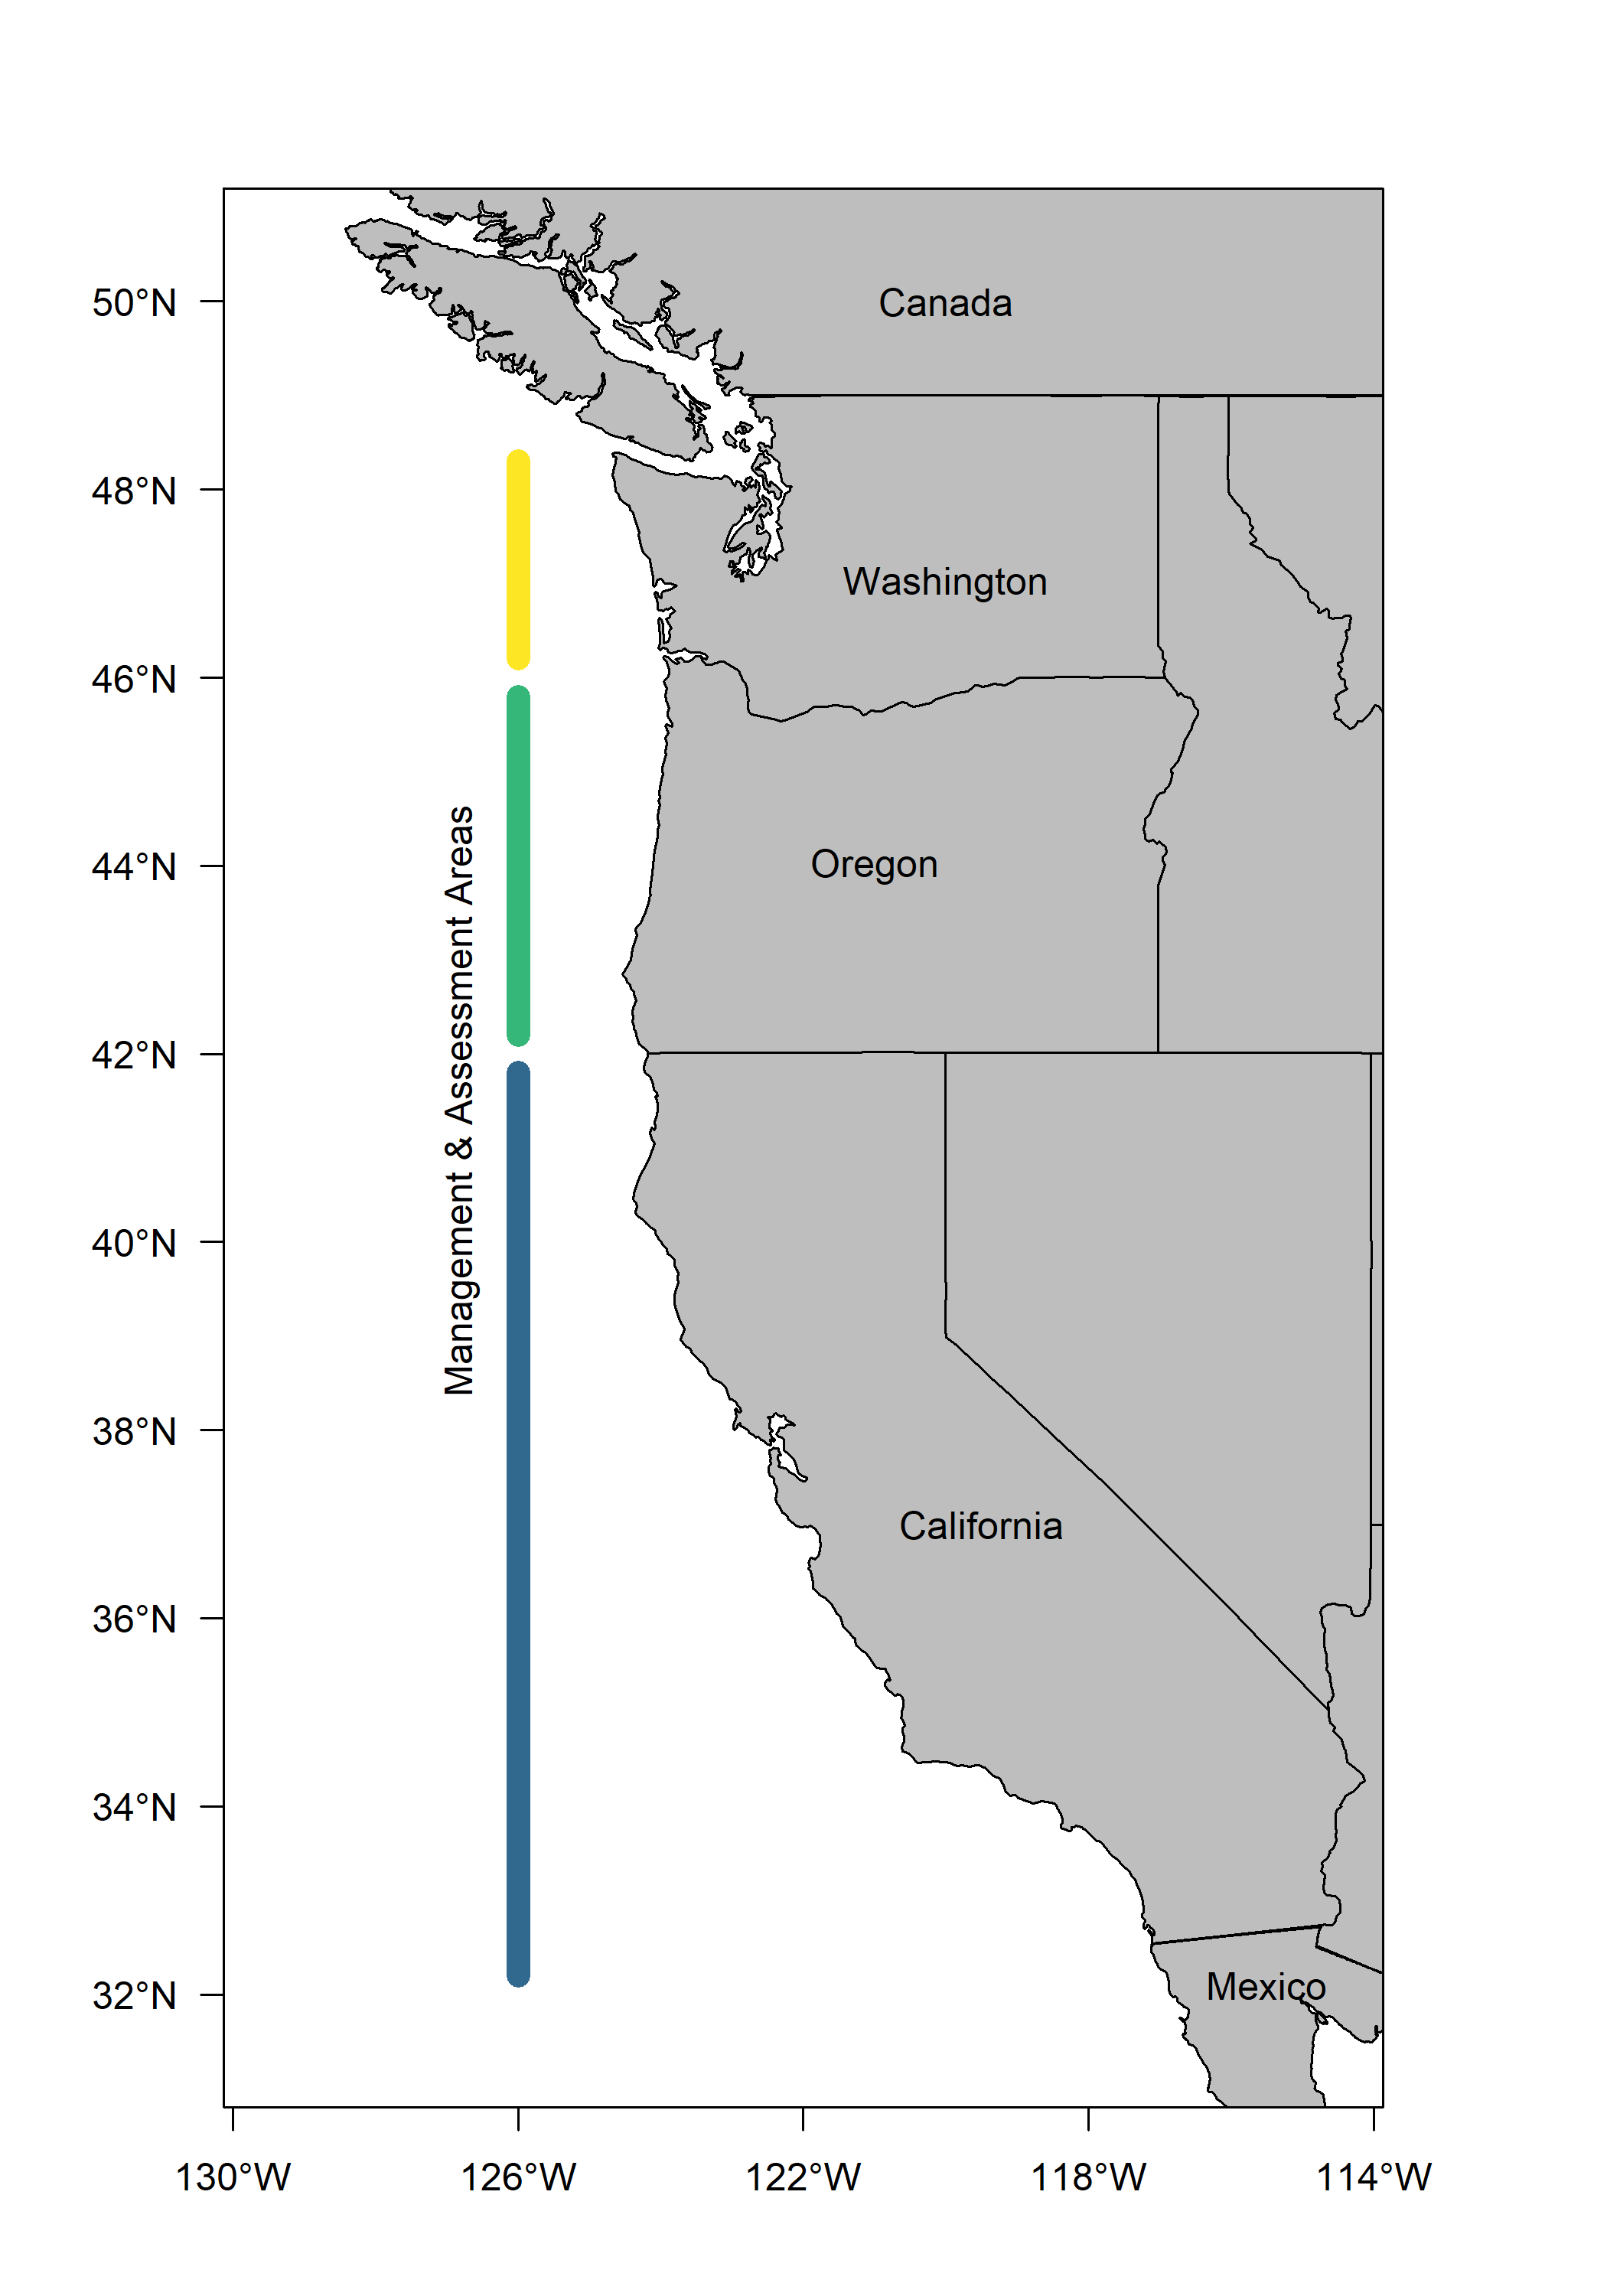
\includegraphics[width=1\textwidth,height=1\textheight]{C:/Users/Jason.Cope/Documents/Github/Sebastes_melanops_OR/Document/figures/stock/black_rockfish_map.png}
\caption{Map of the management and assessment areas for black rockfish.\label{fig:map}}
\end{figure}

\newpage

\begin{figure}
\centering
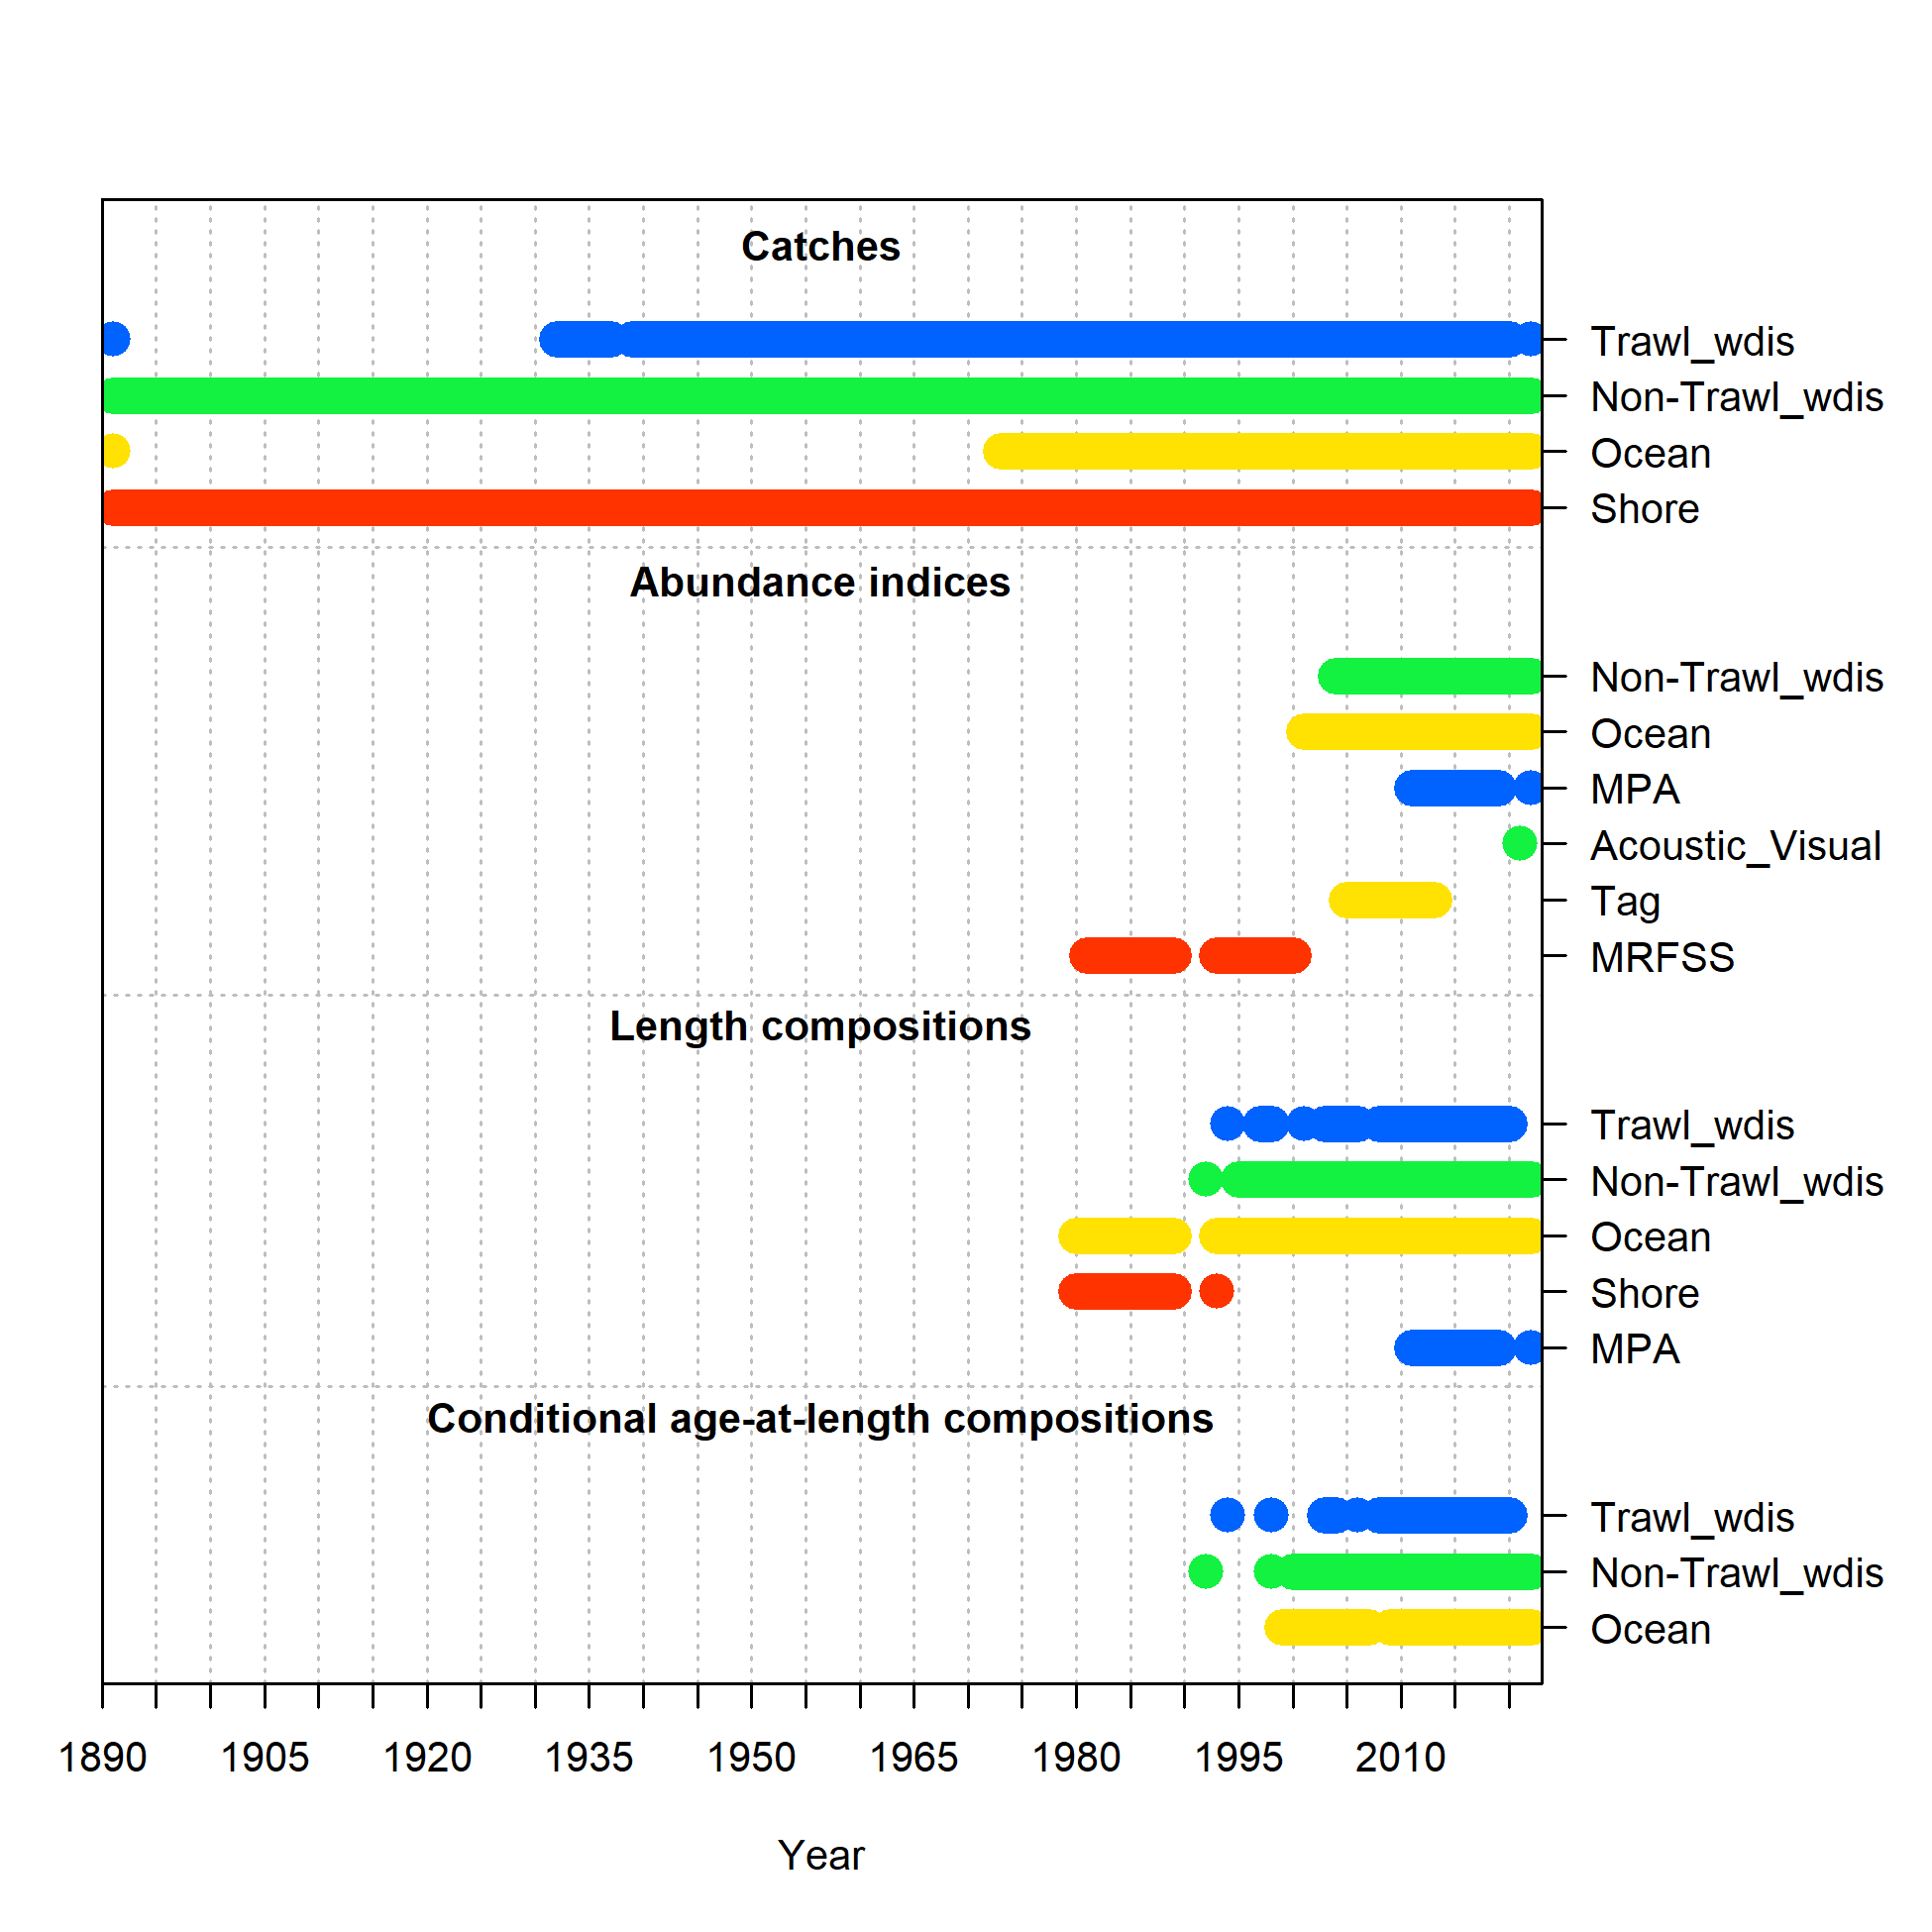
\includegraphics[width=1\textwidth,height=1\textheight]{C:/Users/Jason.Cope/Documents/Github/Sebastes_melanops_OR/Document/models/Reference model/plots/data_plot.png}
\caption{Summary of data sources used in the reference model.\label{fig:data-plot}}
\end{figure}

\newpage

\begin{figure}
\centering
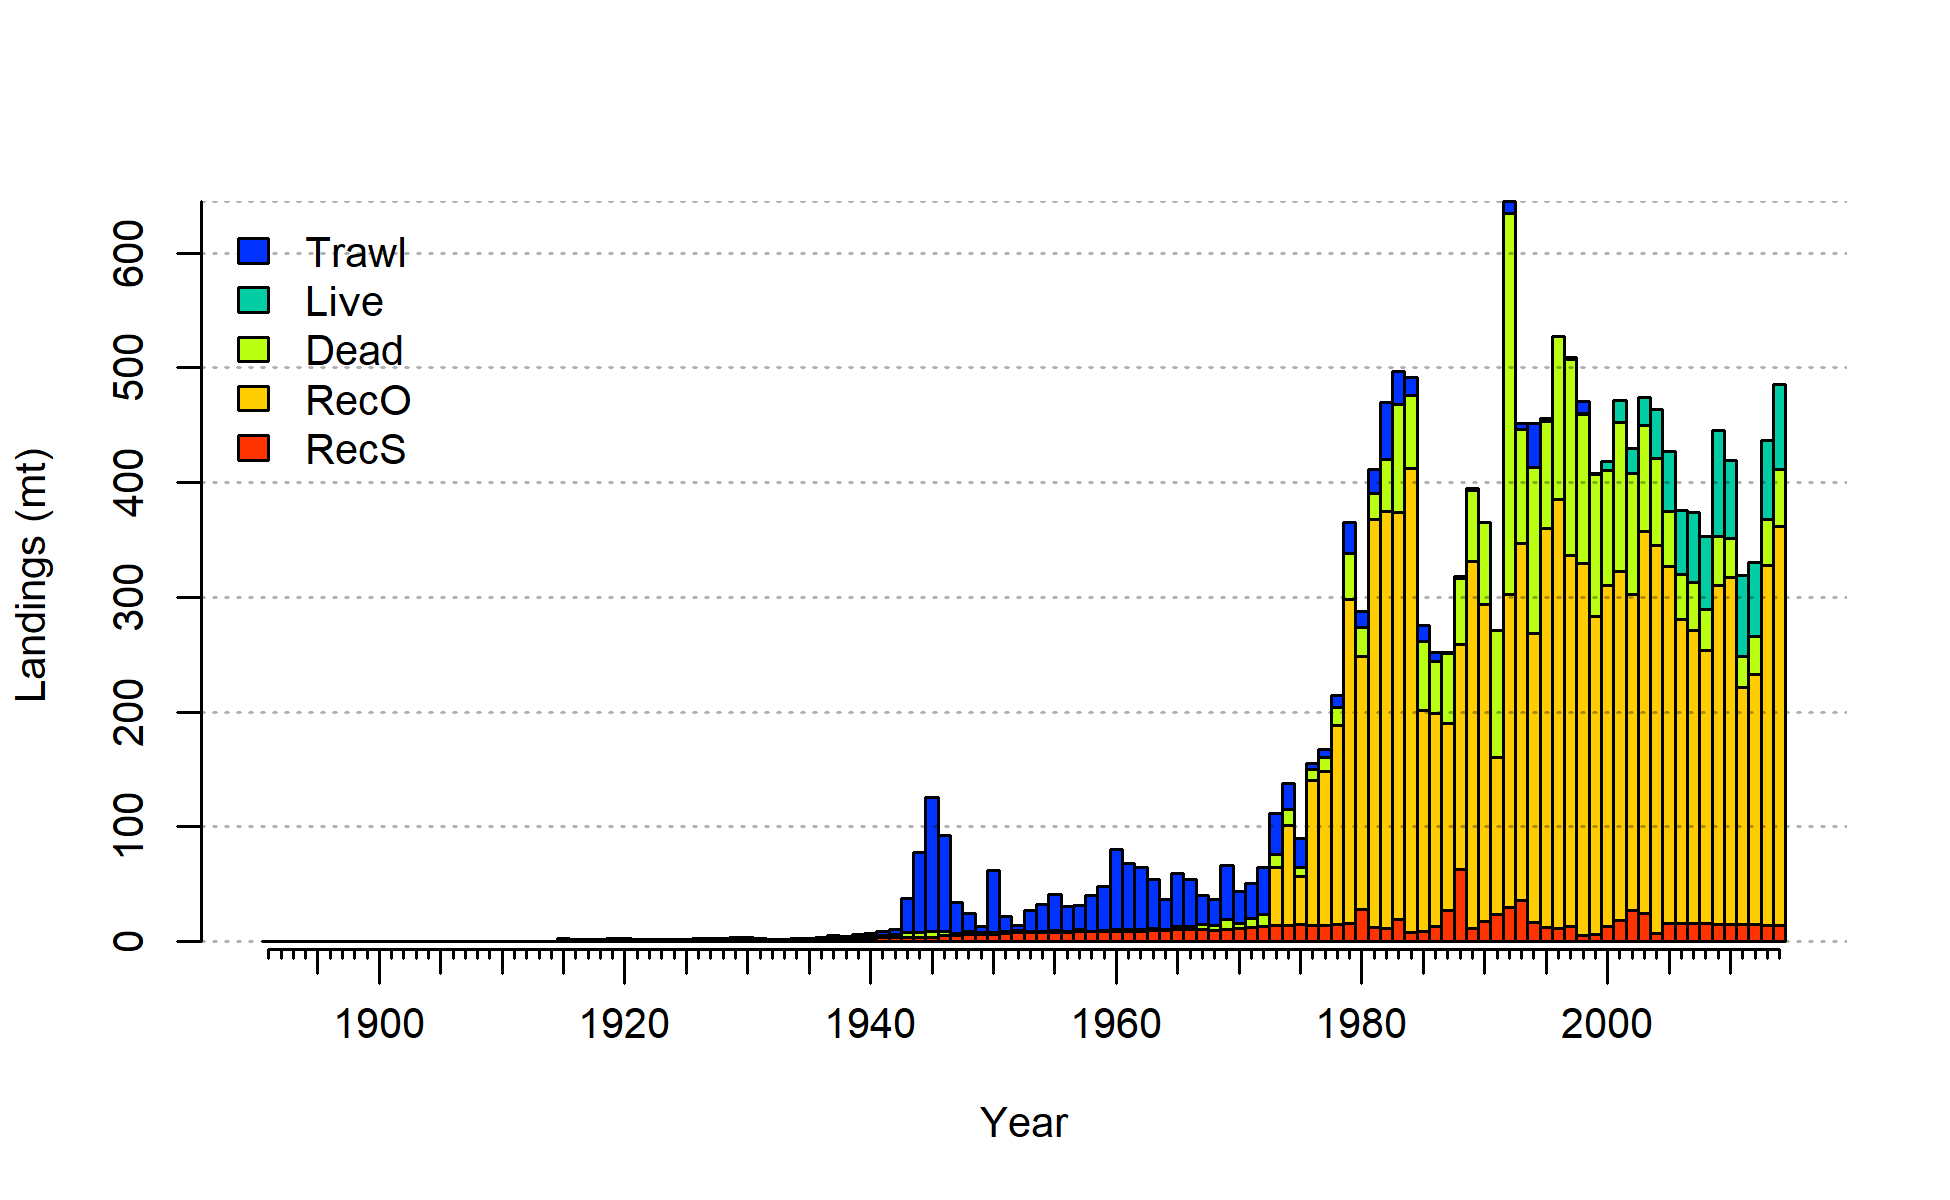
\includegraphics[width=1\textwidth,height=1\textheight]{C:/Users/Jason.Cope/Documents/Github/Sebastes_melanops_OR/Document/models/Reference model/plots/catch2 landings stacked.png}
\caption{Landings by fleet used in the reference model where catches in metric tons by fleet are stacked.\label{fig:catch}}
\end{figure}

\newpage

\begin{figure}
\centering
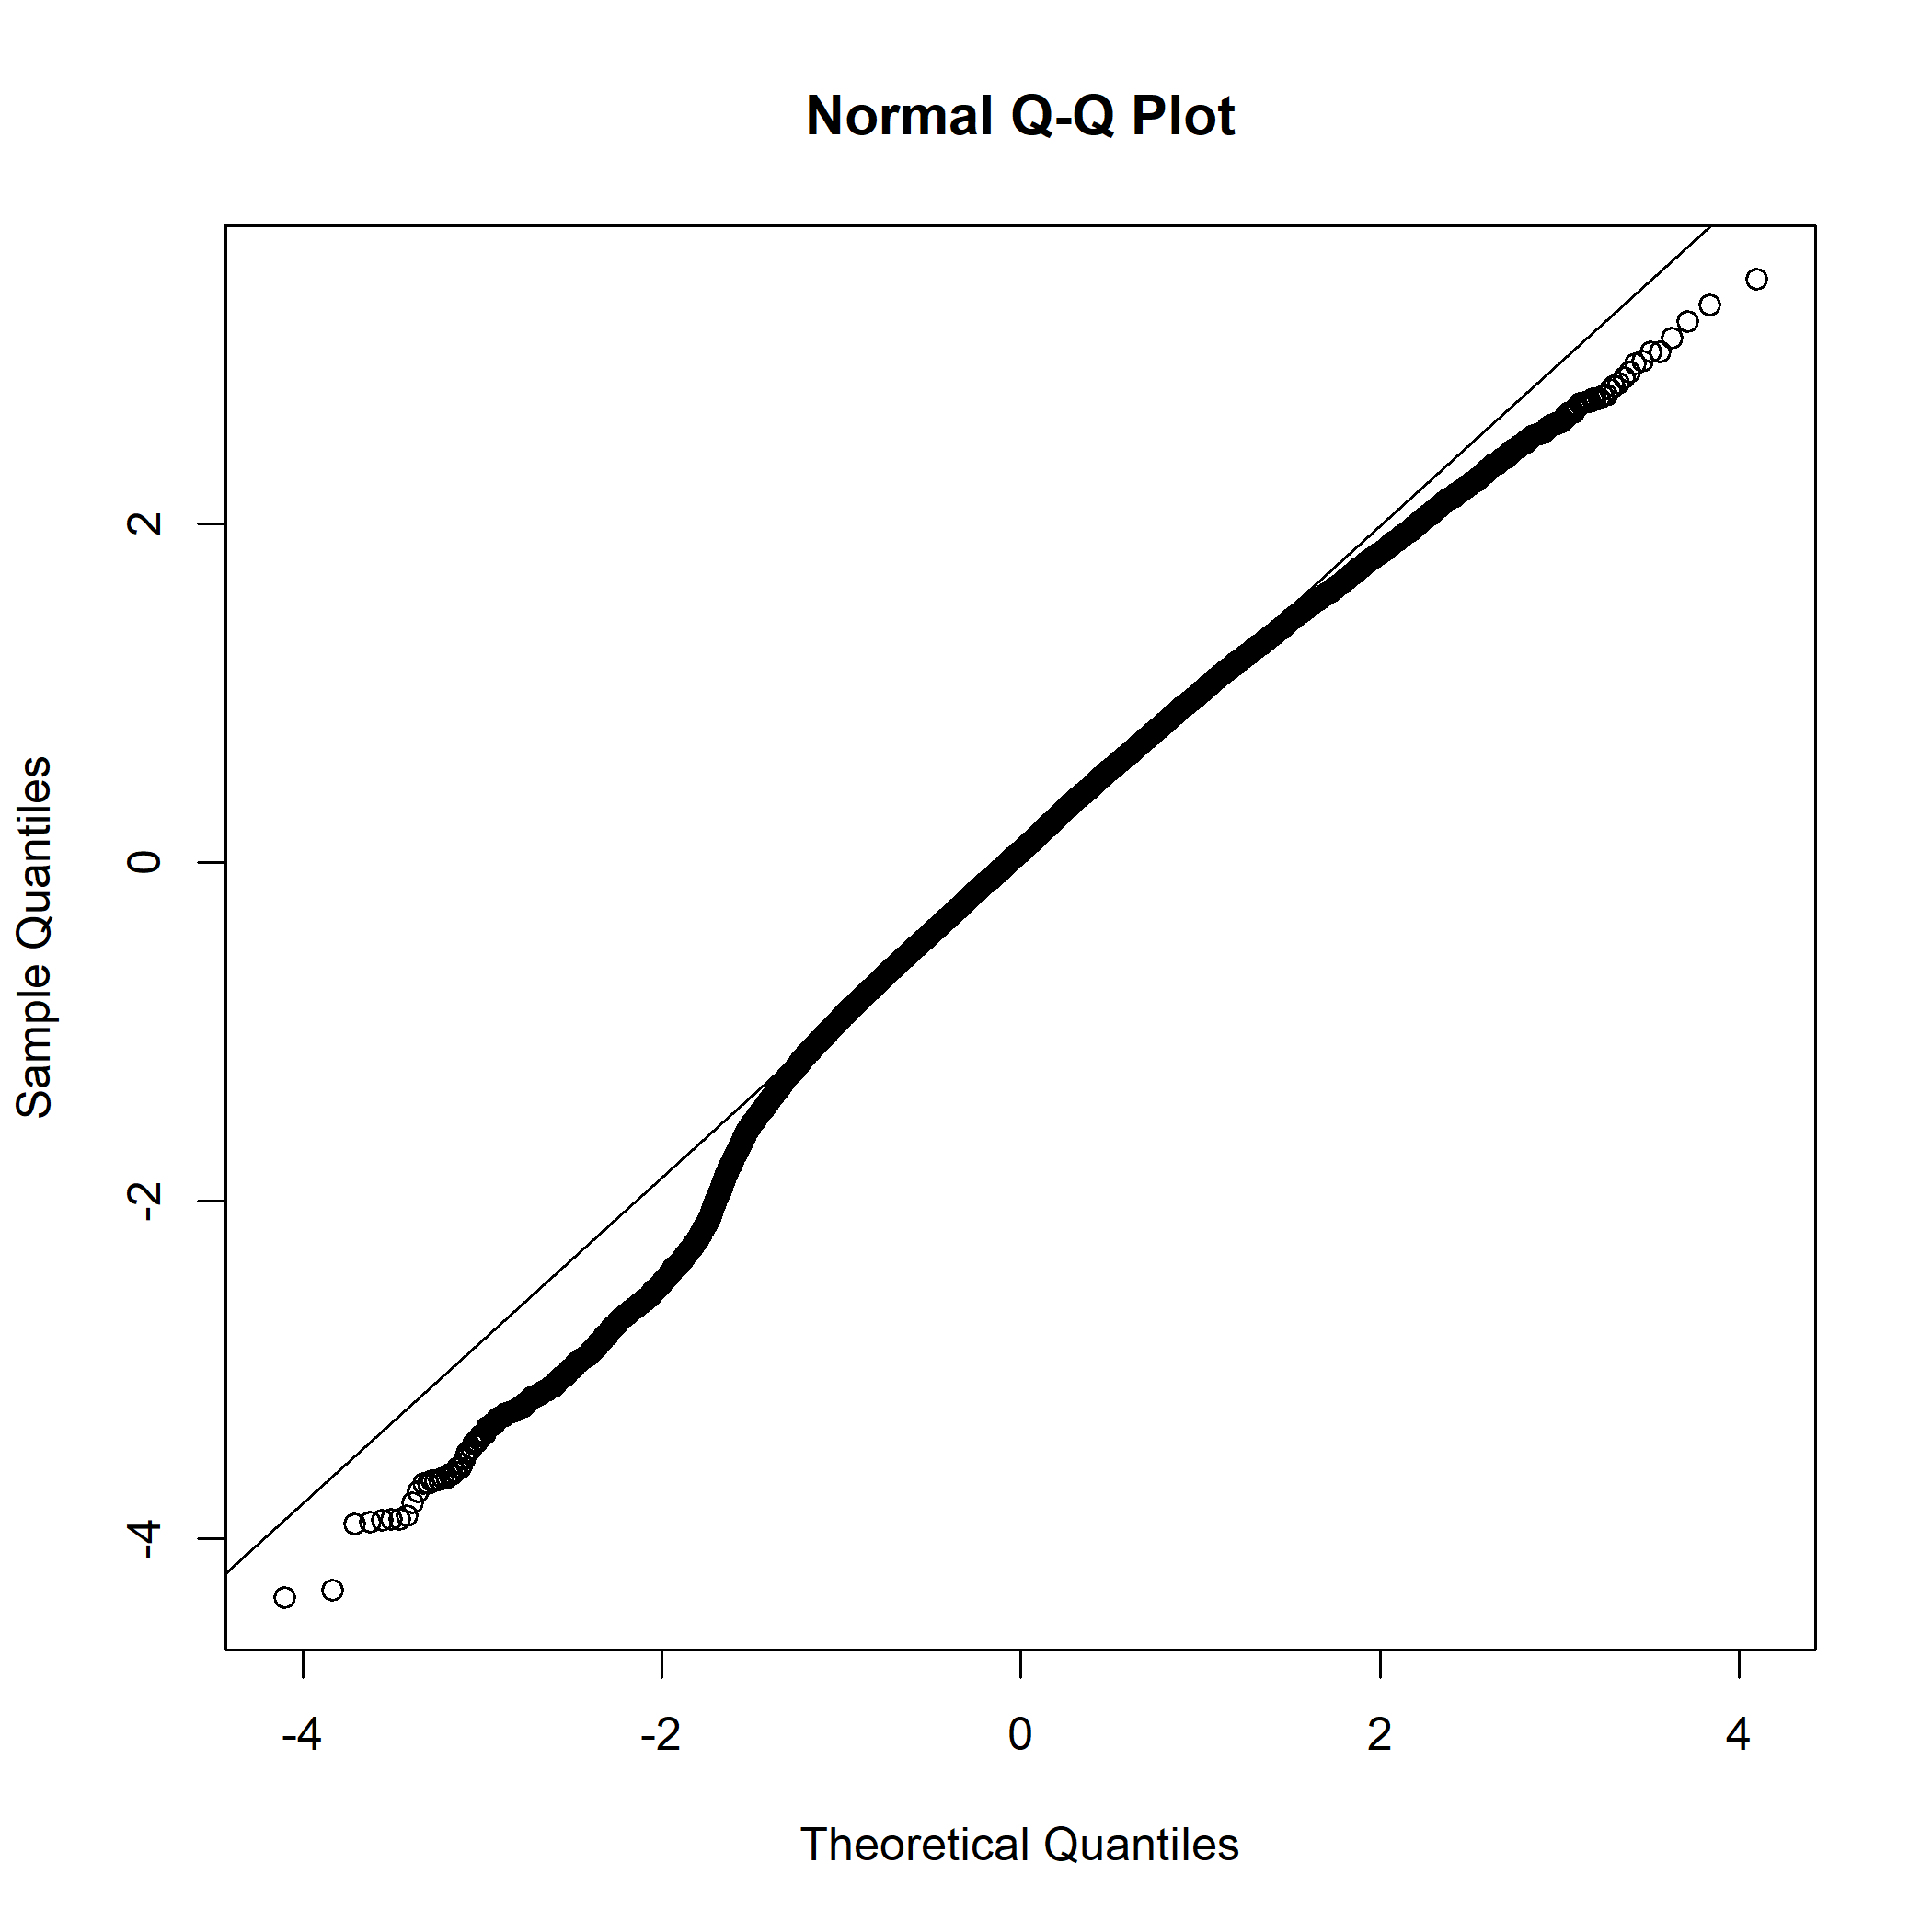
\includegraphics[width=1\textwidth,height=1\textheight]{C:/Users/Jason.Cope/Documents/Github/Sebastes_melanops_OR/Document/figures/index/qq_NSlog.png}
\caption{Q-Q plot for the commercial nearshore logbook index.\label{fig:qq_NSlog}}
\end{figure}

\newpage

\begin{figure}
\centering
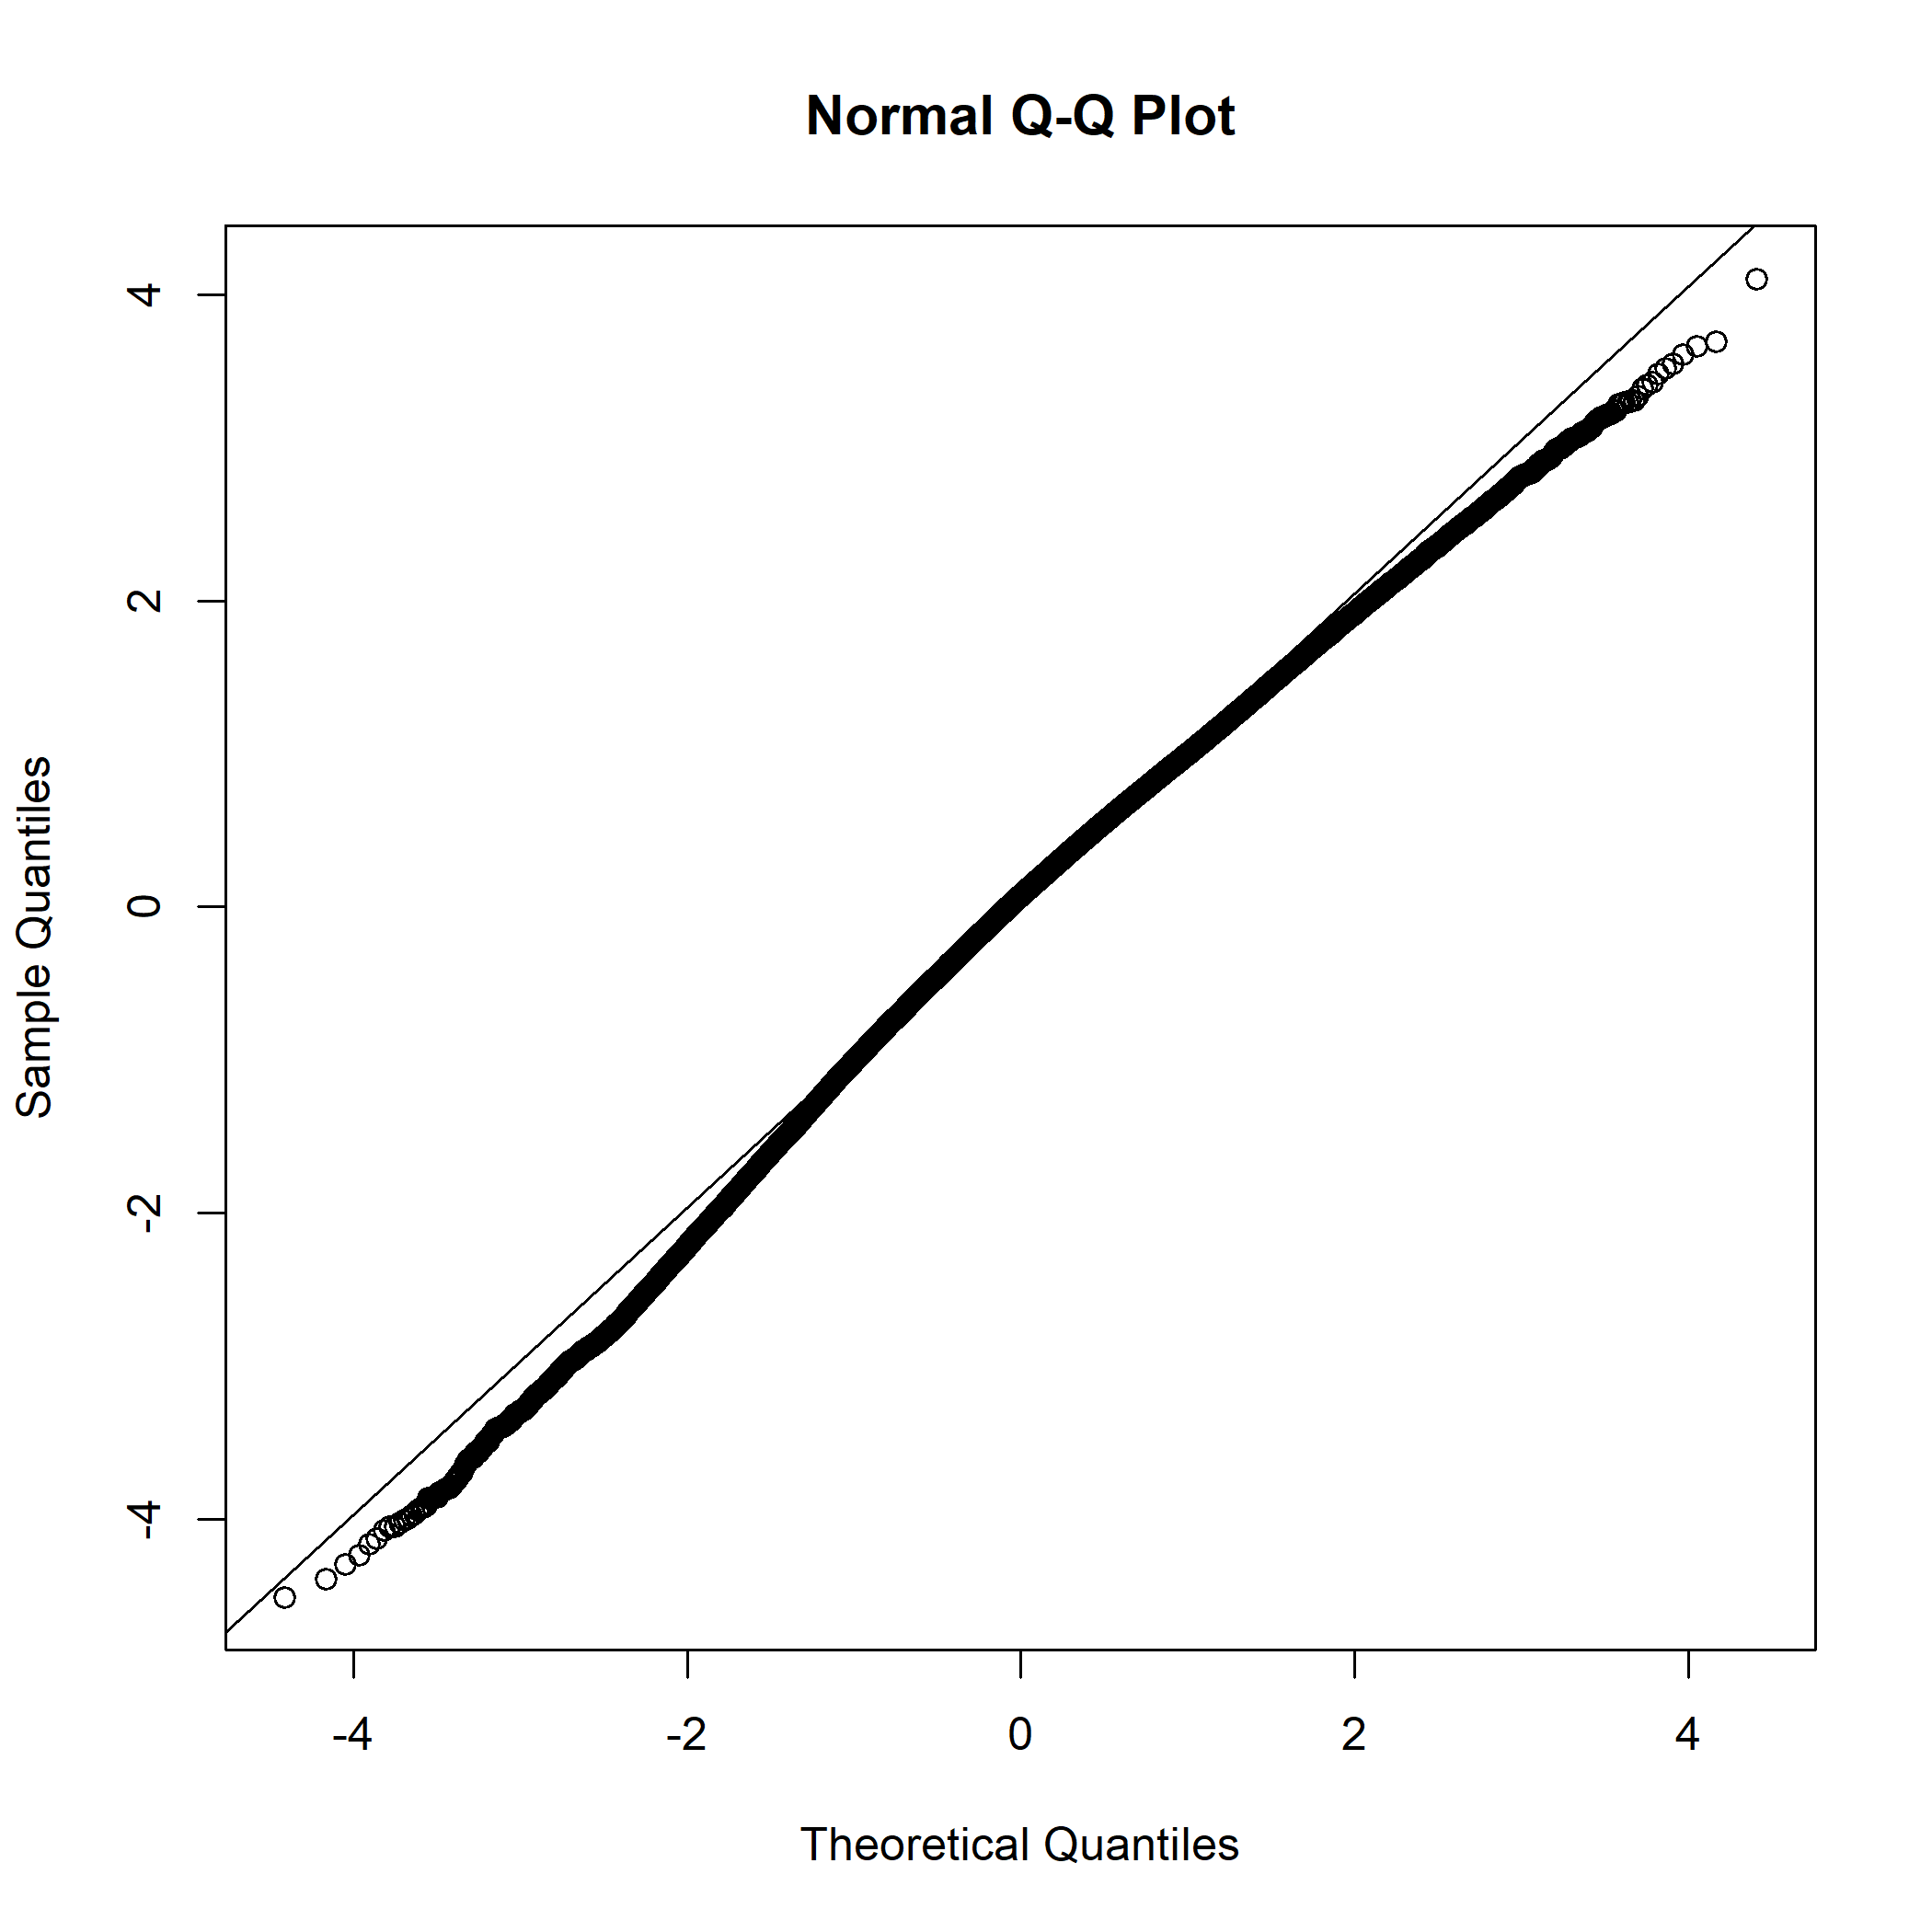
\includegraphics[width=1\textwidth,height=1\textheight]{C:/Users/Jason.Cope/Documents/Github/Sebastes_melanops_OR/Document/figures/index/qq_ORBS.png}
\caption{Q-Q plot for the recreational ORBS index.\label{fig:qq_ORBS}}
\end{figure}

\newpage

\hypertarget{biology}{%
\subsection{Biology}\label{biology}}

\begin{figure}
\centering
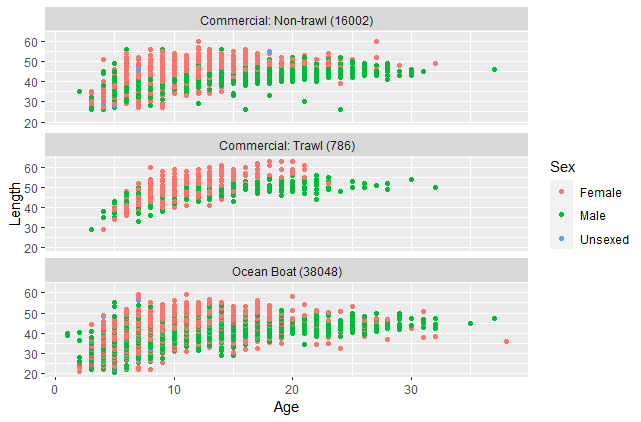
\includegraphics[width=1\textwidth,height=1\textheight]{C:/Users/Jason.Cope/Documents/Github/Sebastes_melanops_OR/Document/figures/biology_plots/OR_AG_Source_Sex.png}
\caption{Observed length-at-age by data source and sex.\label{fig:len-age-data-sex}}
\end{figure}

\newpage

\begin{figure}
\centering
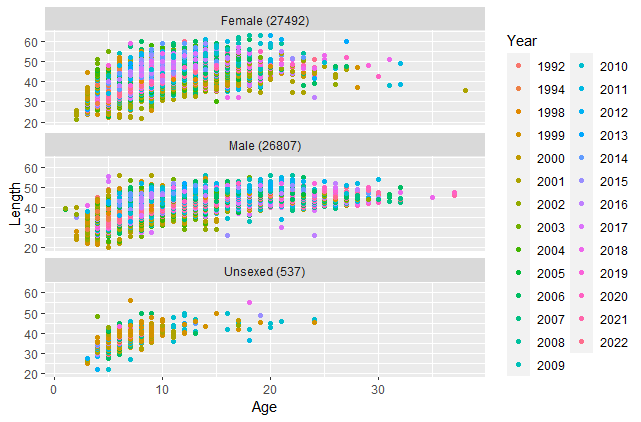
\includegraphics[width=1\textwidth,height=1\textheight]{C:/Users/Jason.Cope/Documents/Github/Sebastes_melanops_OR/Document/figures/biology_plots/OR_AG_Sex_Year.png}
\caption{Observed length-at-age by sex and year. Total samples are indicated in parentheses.\label{fig:len-age-sex-year}}
\end{figure}

\newpage

\begin{figure}
\centering
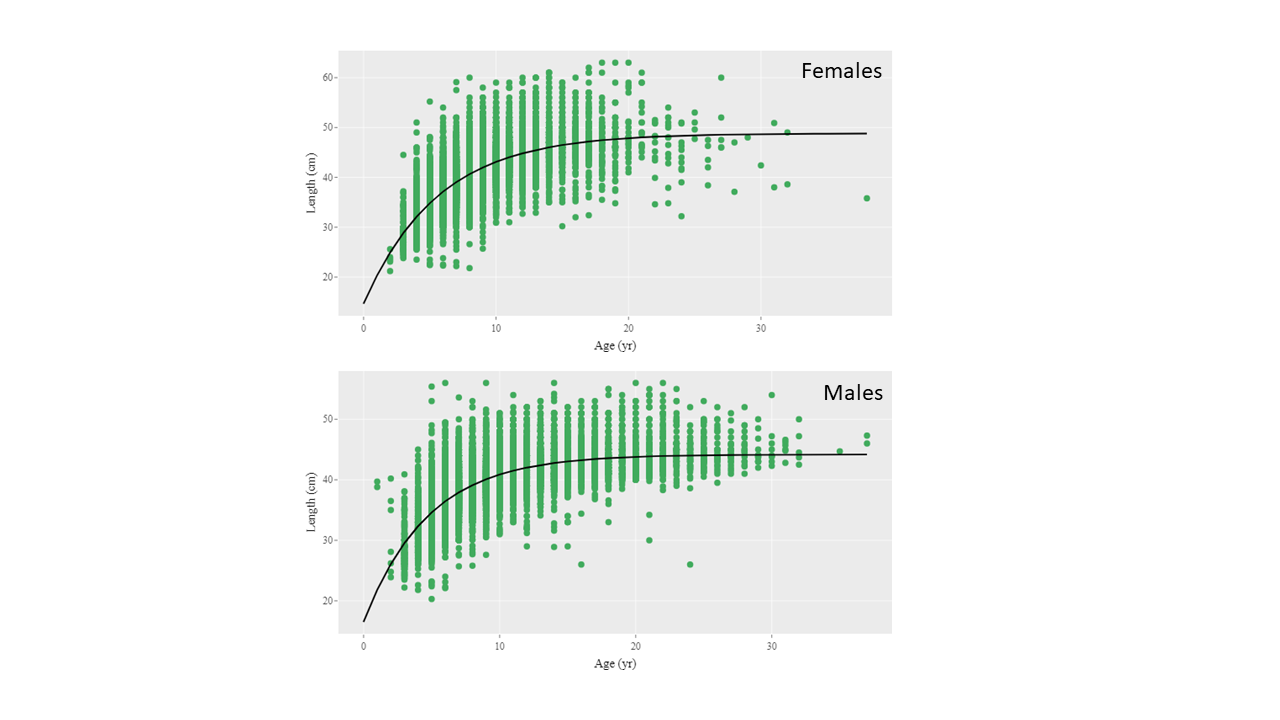
\includegraphics[width=1\textwidth,height=1\textheight]{C:/Users/Jason.Cope/Documents/Github/Sebastes_melanops_OR/Document/figures/biology_plots/OR_VBGF_fit.png}
\caption{External fits to the observed length-at-age by sex.\label{fig:len-age-fit}}
\end{figure}

\newpage

\begin{figure}
\centering
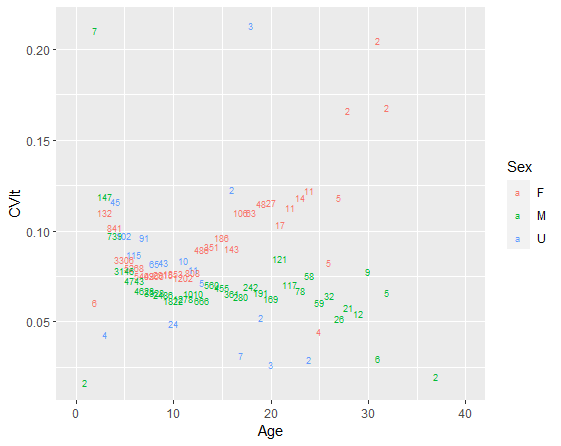
\includegraphics[width=1\textwidth,height=1\textheight]{C:/Users/Jason.Cope/Documents/Github/Sebastes_melanops_OR/Document/figures/biology_plots/OR_CV_Sex_plot.png}
\caption{Coefficient of variation of length by age by sex. Numbers indicate samples by age and colors indicate sex.\label{fig:cv-lt-age}}
\end{figure}

\newpage

\begin{figure}
\centering
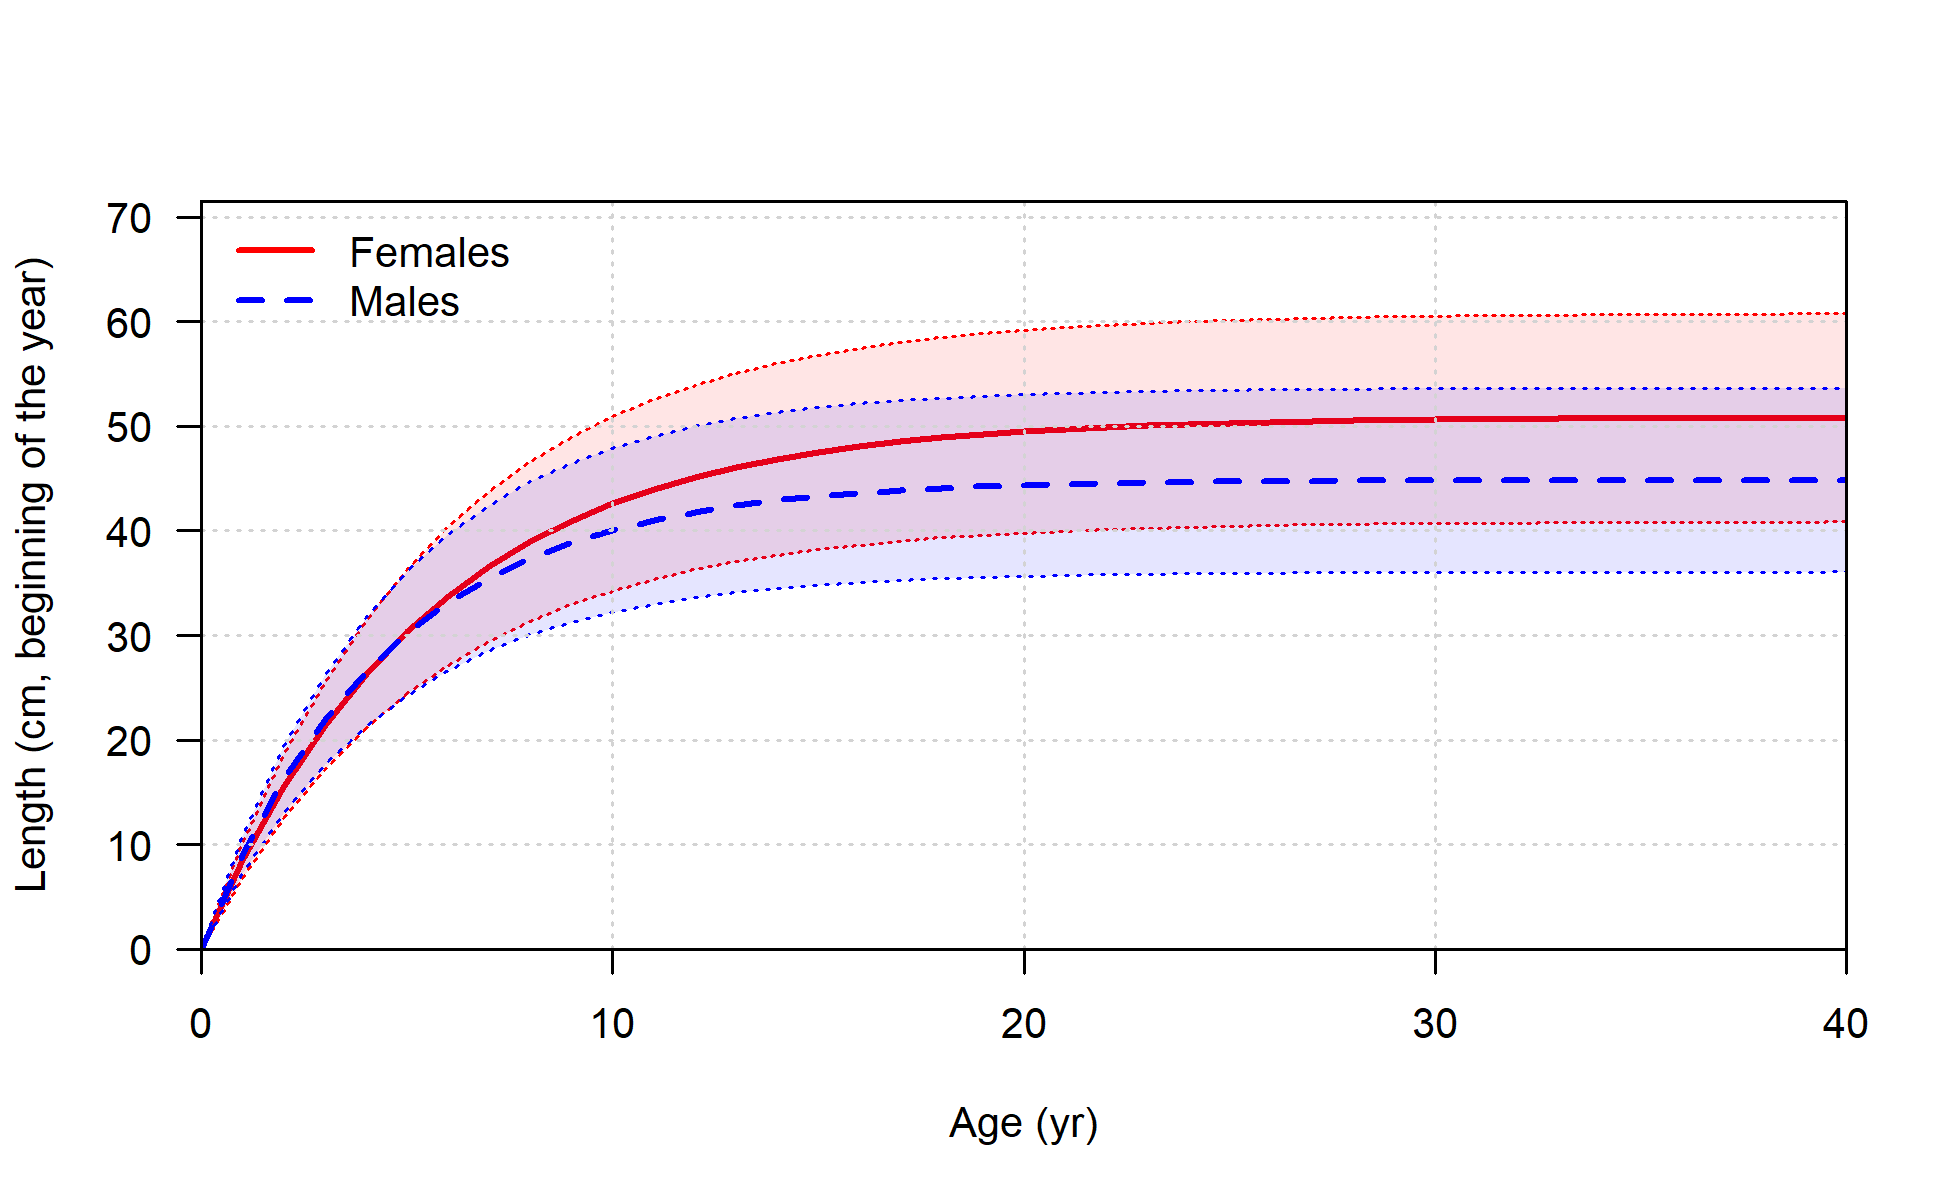
\includegraphics[width=1\textwidth,height=1\textheight]{C:/Users/Jason.Cope/Documents/Github/Sebastes_melanops_OR/Document/models/Reference model/plots/bio1_sizeatage.png}
\caption{Model estimated length-at-age. Shaded area indicates 95 percent distribution of length-at-age around the estimated growth curve.\label{fig:len-age-ss}}
\end{figure}

\clearpage

\begin{figure}
\centering
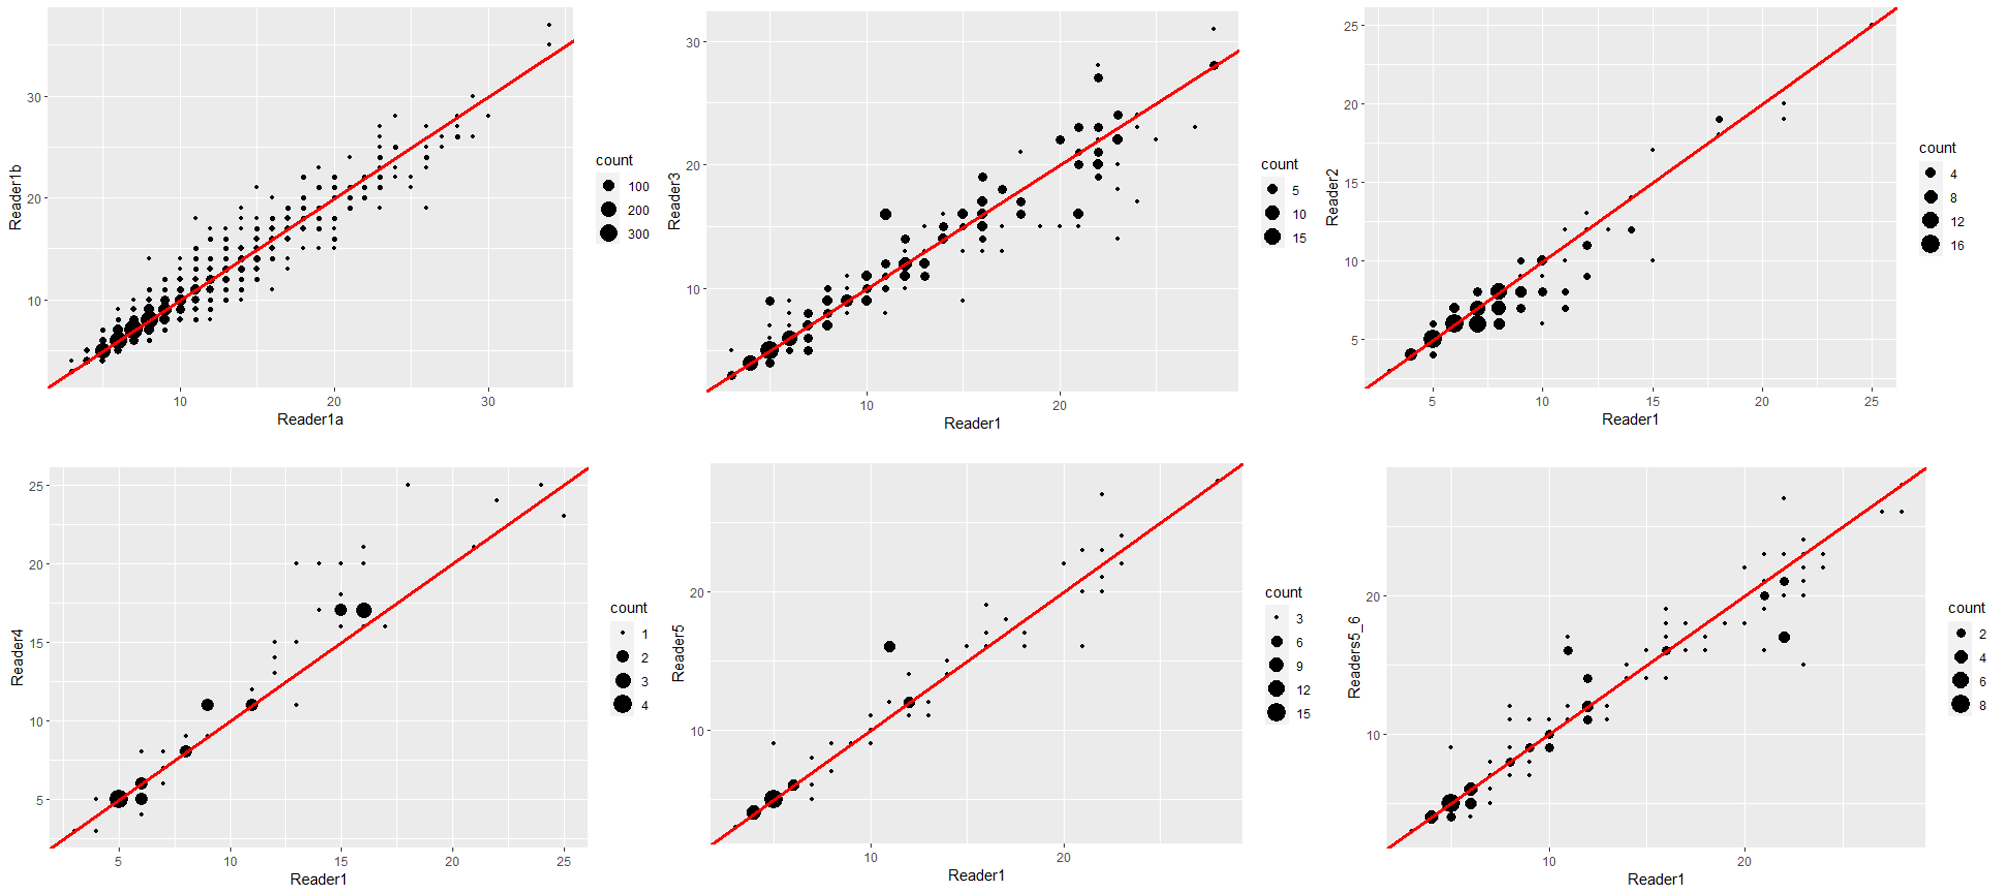
\includegraphics[width=1\textwidth,height=1\textheight]{C:/Users/Jason.Cope/Documents/Github/Sebastes_melanops_OR/Document/figures/biology_plots/Age1_1plots.png}
\caption{Ageing bias plots by reader comparisons.\label{fig:age1-plot}}
\end{figure}

\newpage

\begin{figure}
\centering
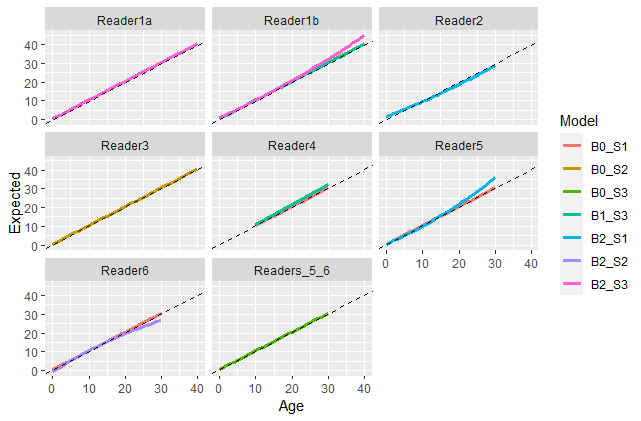
\includegraphics[width=1\textwidth,height=1\textheight]{C:/Users/Jason.Cope/Documents/Github/Sebastes_melanops_OR/Document/figures/biology_plots/OR_Reader_Bias_plot.png}
\caption{Estimated bias relationships for each considered matrix. Reader 1 is always considered unbiased. Reader 1a and 1b is an intra-reader comparison. B refers to the bias type and S refers to the imprecision type in the model selection for the ageing error matrix.\label{fig:age-error-bias}}
\end{figure}

\newpage

\begin{figure}
\centering
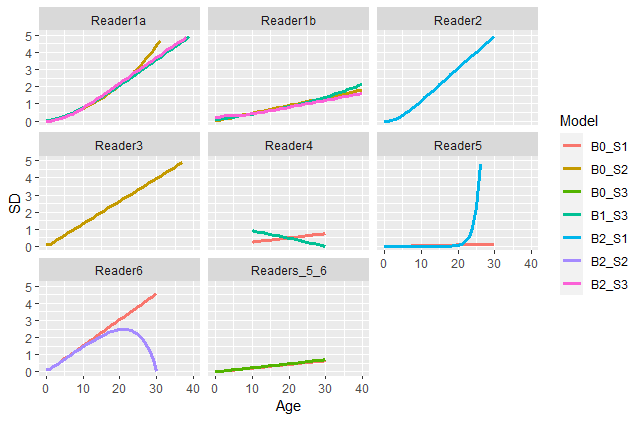
\includegraphics[width=1\textwidth,height=1\textheight]{C:/Users/Jason.Cope/Documents/Github/Sebastes_melanops_OR/Document/figures/biology_plots/OR_Reader_SD_plot.png}
\caption{Ageing error matrix standard deviation (SD) values by comparison. B refers to the bias type and S refers to the imprecision type in the model selection for the ageing error matrix.\label{fig:age-error-sd}}
\end{figure}

\newpage

\begin{figure}
\centering
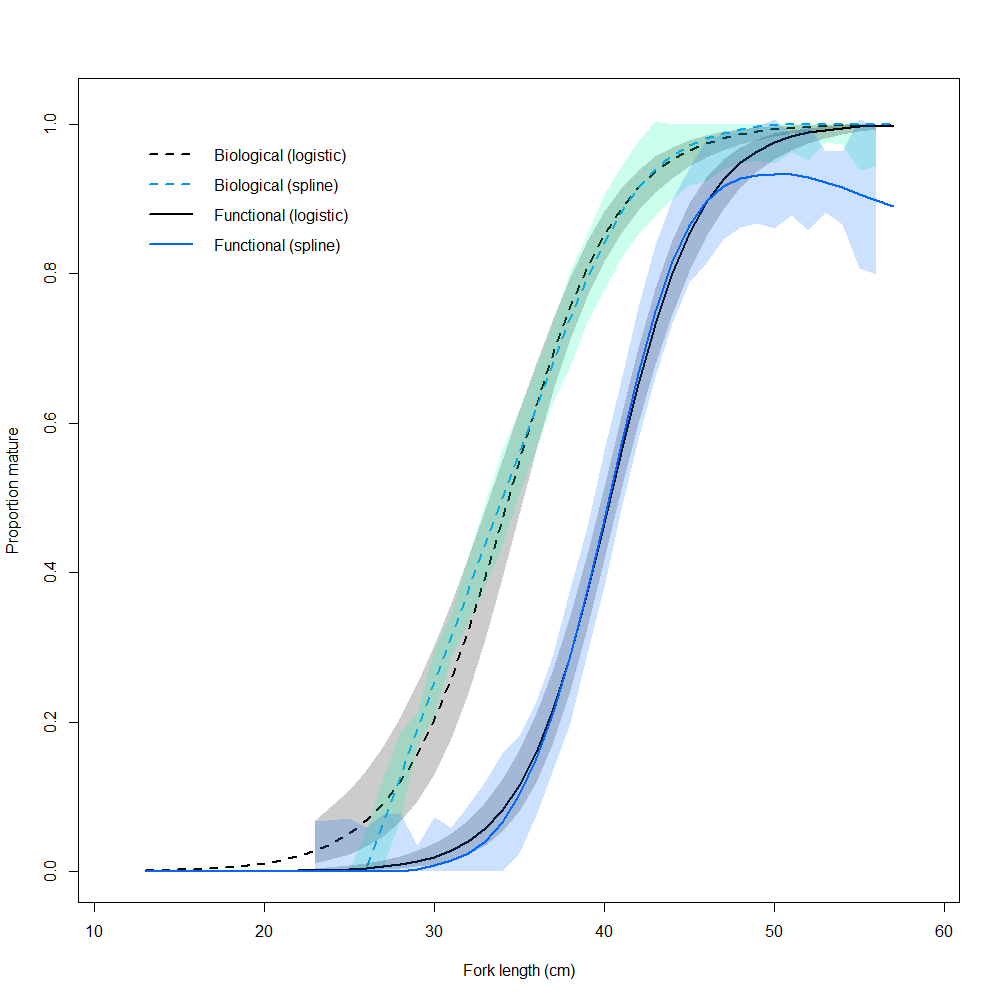
\includegraphics[width=1\textwidth,height=1\textheight]{C:/Users/Jason.Cope/Documents/Github/Sebastes_melanops_OR/Document/figures/biology_plots/Fig1_bio_and_func_color.png}
\caption{Biological and functional maturity ogives. Biological maturity ogives are represented by the dashed lines (logistic regression and 95\% CI is grey, flexible spline and 95\% CI is light green). Functional maturity ogives are represented by the solid lines (logistic regression and 95\% CI is grey, flexible spline and 95\% CI is light blue).\label{fig:bio-fxn-mat-color}}
\end{figure}

\newpage

\begin{figure}
\centering
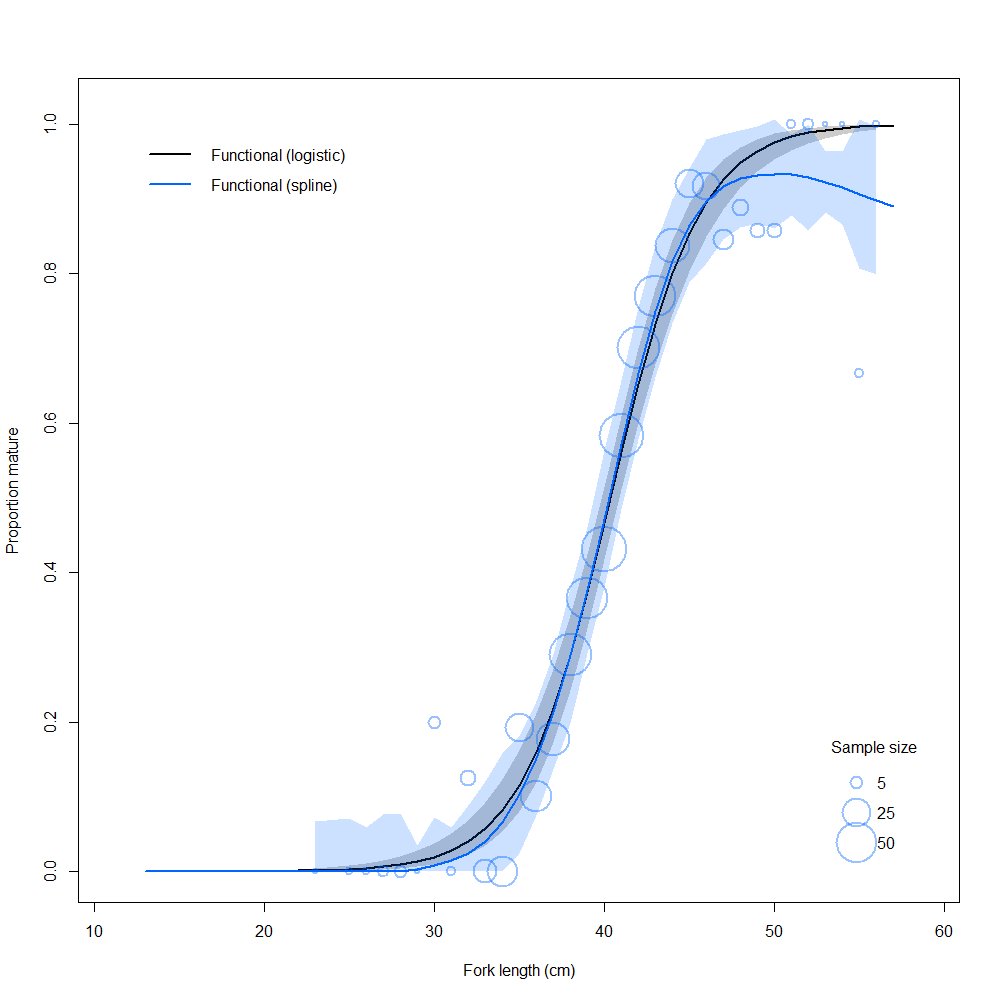
\includegraphics[width=1\textwidth,height=1\textheight]{C:/Users/Jason.Cope/Documents/Github/Sebastes_melanops_OR/Document/figures/biology_plots/Fig2_func_samplesize_color.png}
\caption{Functional maturity ogives and sample size. Functional maturity ogives are represented by the solid lines (logistic regression and 95\% CI is grey, flexible spline and 95\% CI is light blue) and sample size is denoted by the size of the bubbles).\label{fig:fxn-spline-mat-color}}
\end{figure}

\newpage

\begin{figure}
\centering
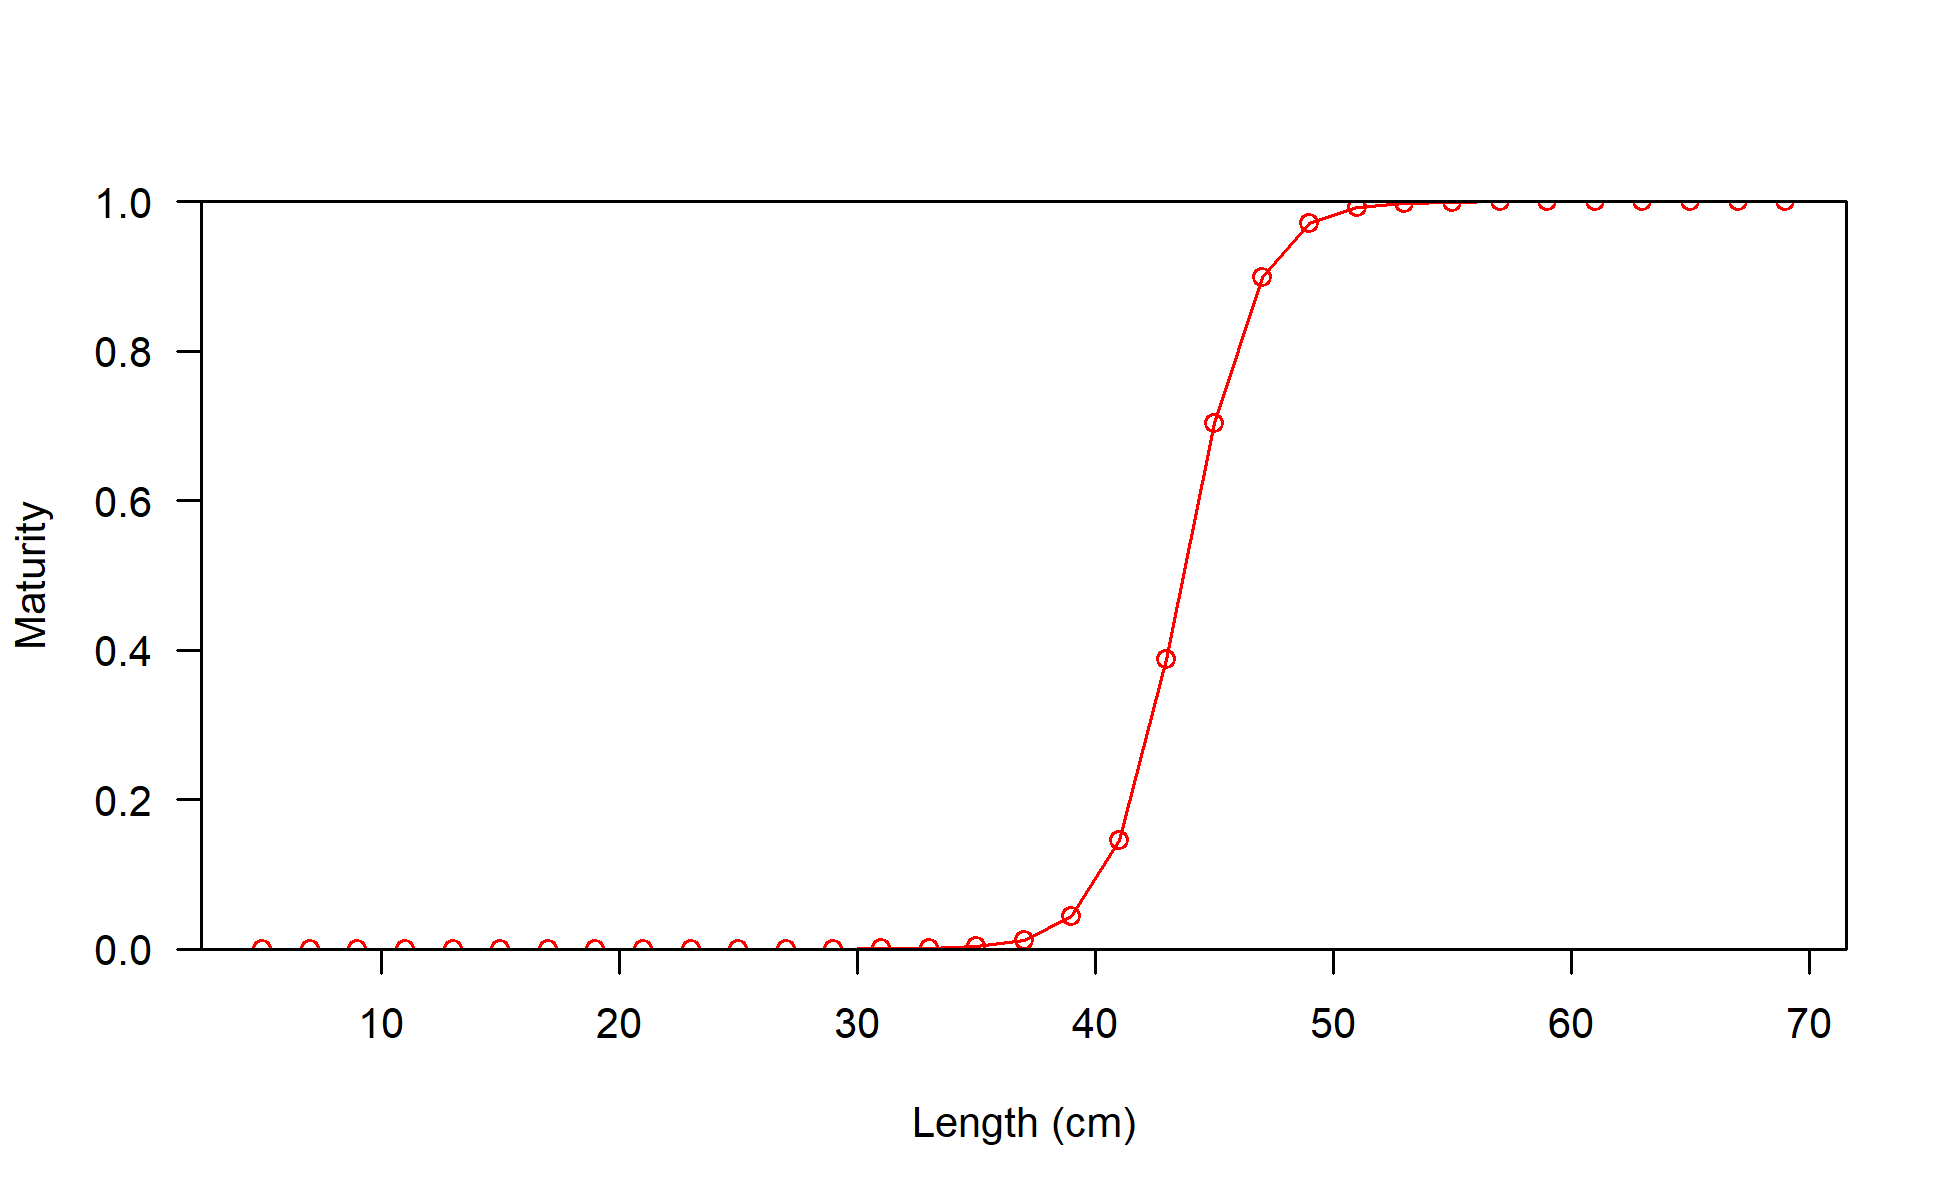
\includegraphics[width=1\textwidth,height=1\textheight]{C:/Users/Jason.Cope/Documents/Github/Sebastes_melanops_OR/Document/models/Reference model/plots/bio6_maturity.png}
\caption{Maturity as a function of length (cm) used in the base model.\label{fig:maturity}}
\end{figure}

\newpage

\begin{figure}
\centering
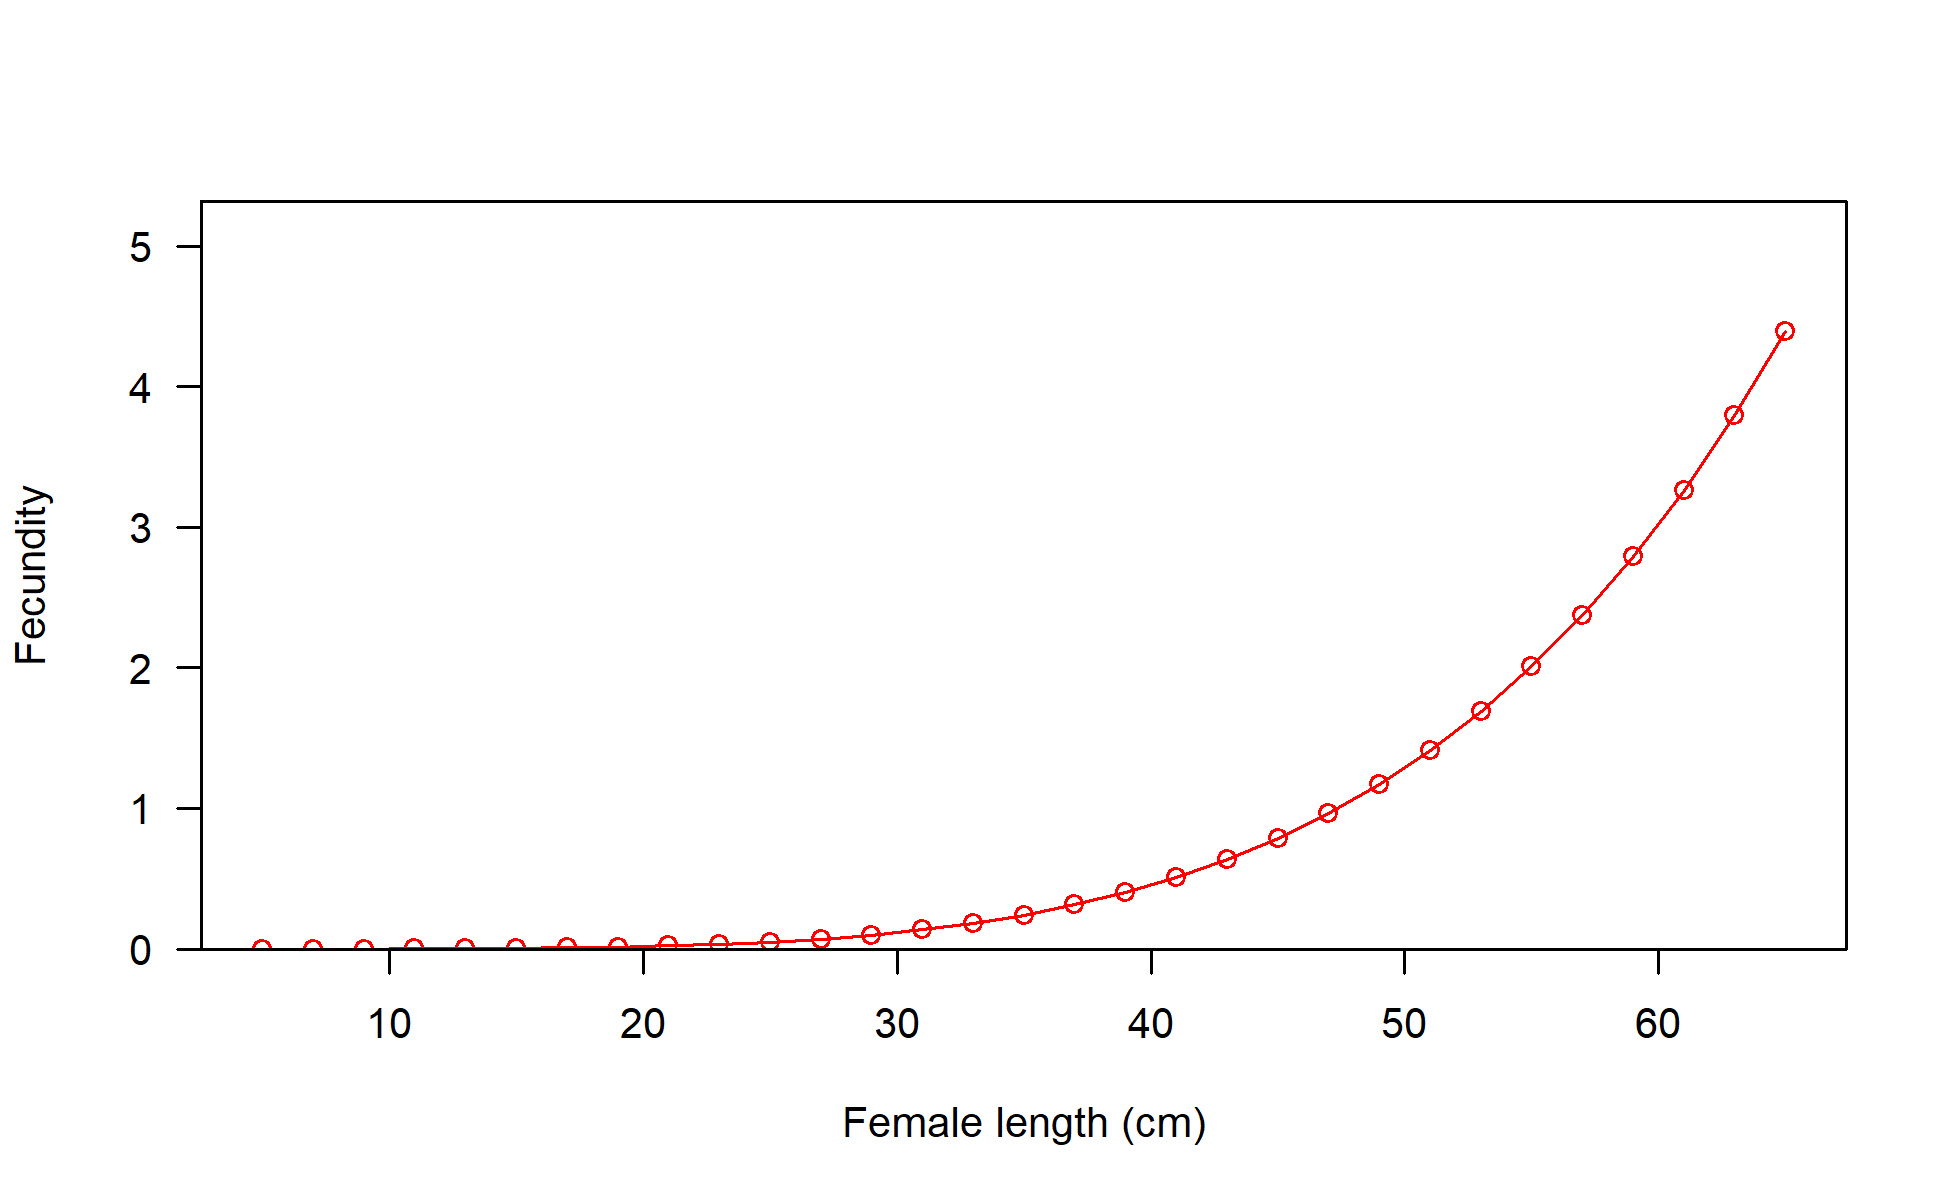
\includegraphics[width=1\textwidth,height=1\textheight]{C:/Users/Jason.Cope/Documents/Github/Sebastes_melanops_OR/Document/models/Reference model/plots/bio9_fecundity_len.png}
\caption{Fecundity (kg) as a function of length (cm) used in the base model.\label{fig:fecundity}}
\end{figure}

\newpage

\begin{figure}
\centering
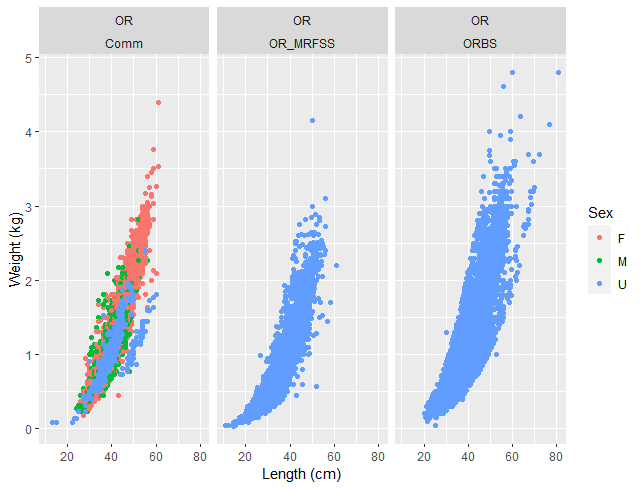
\includegraphics[width=1\textwidth,height=1\textheight]{C:/Users/Jason.Cope/Documents/Github/Sebastes_melanops_OR/Document/figures/biology_plots/LW_OR_State_Source_Sex.png}
\caption{Sex-specific length (cm)-weight (kg) data for Oregon black rockfish samples by source. MRFSS and ORBS are the ocean boat recreational fishery from early and late periods.\label{fig:len-weight-data}}
\end{figure}

\newpage

\begin{figure}
\centering
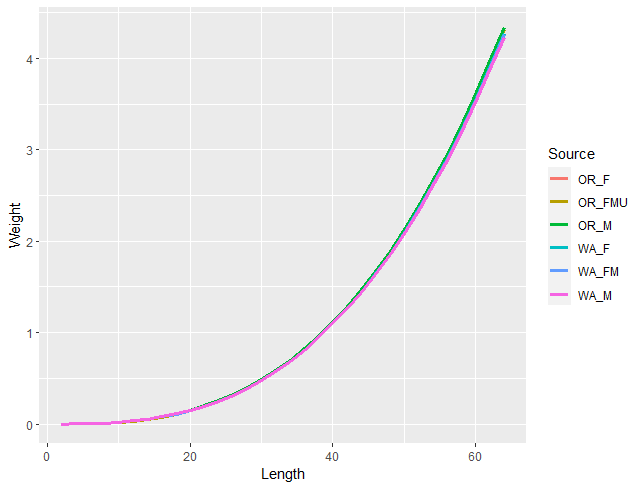
\includegraphics[width=1\textwidth,height=1\textheight]{C:/Users/Jason.Cope/Documents/Github/Sebastes_melanops_OR/Document/figures/biology_plots/LW_lines_States_Sex.png}
\caption{Sex-specific length (cm)-weight (kg) estimated power function relationships. Washington state estimate relationships are also provided for comparison.\label{fig:len-weight-or-wa}}
\end{figure}

\clearpage

\begin{figure}
\centering
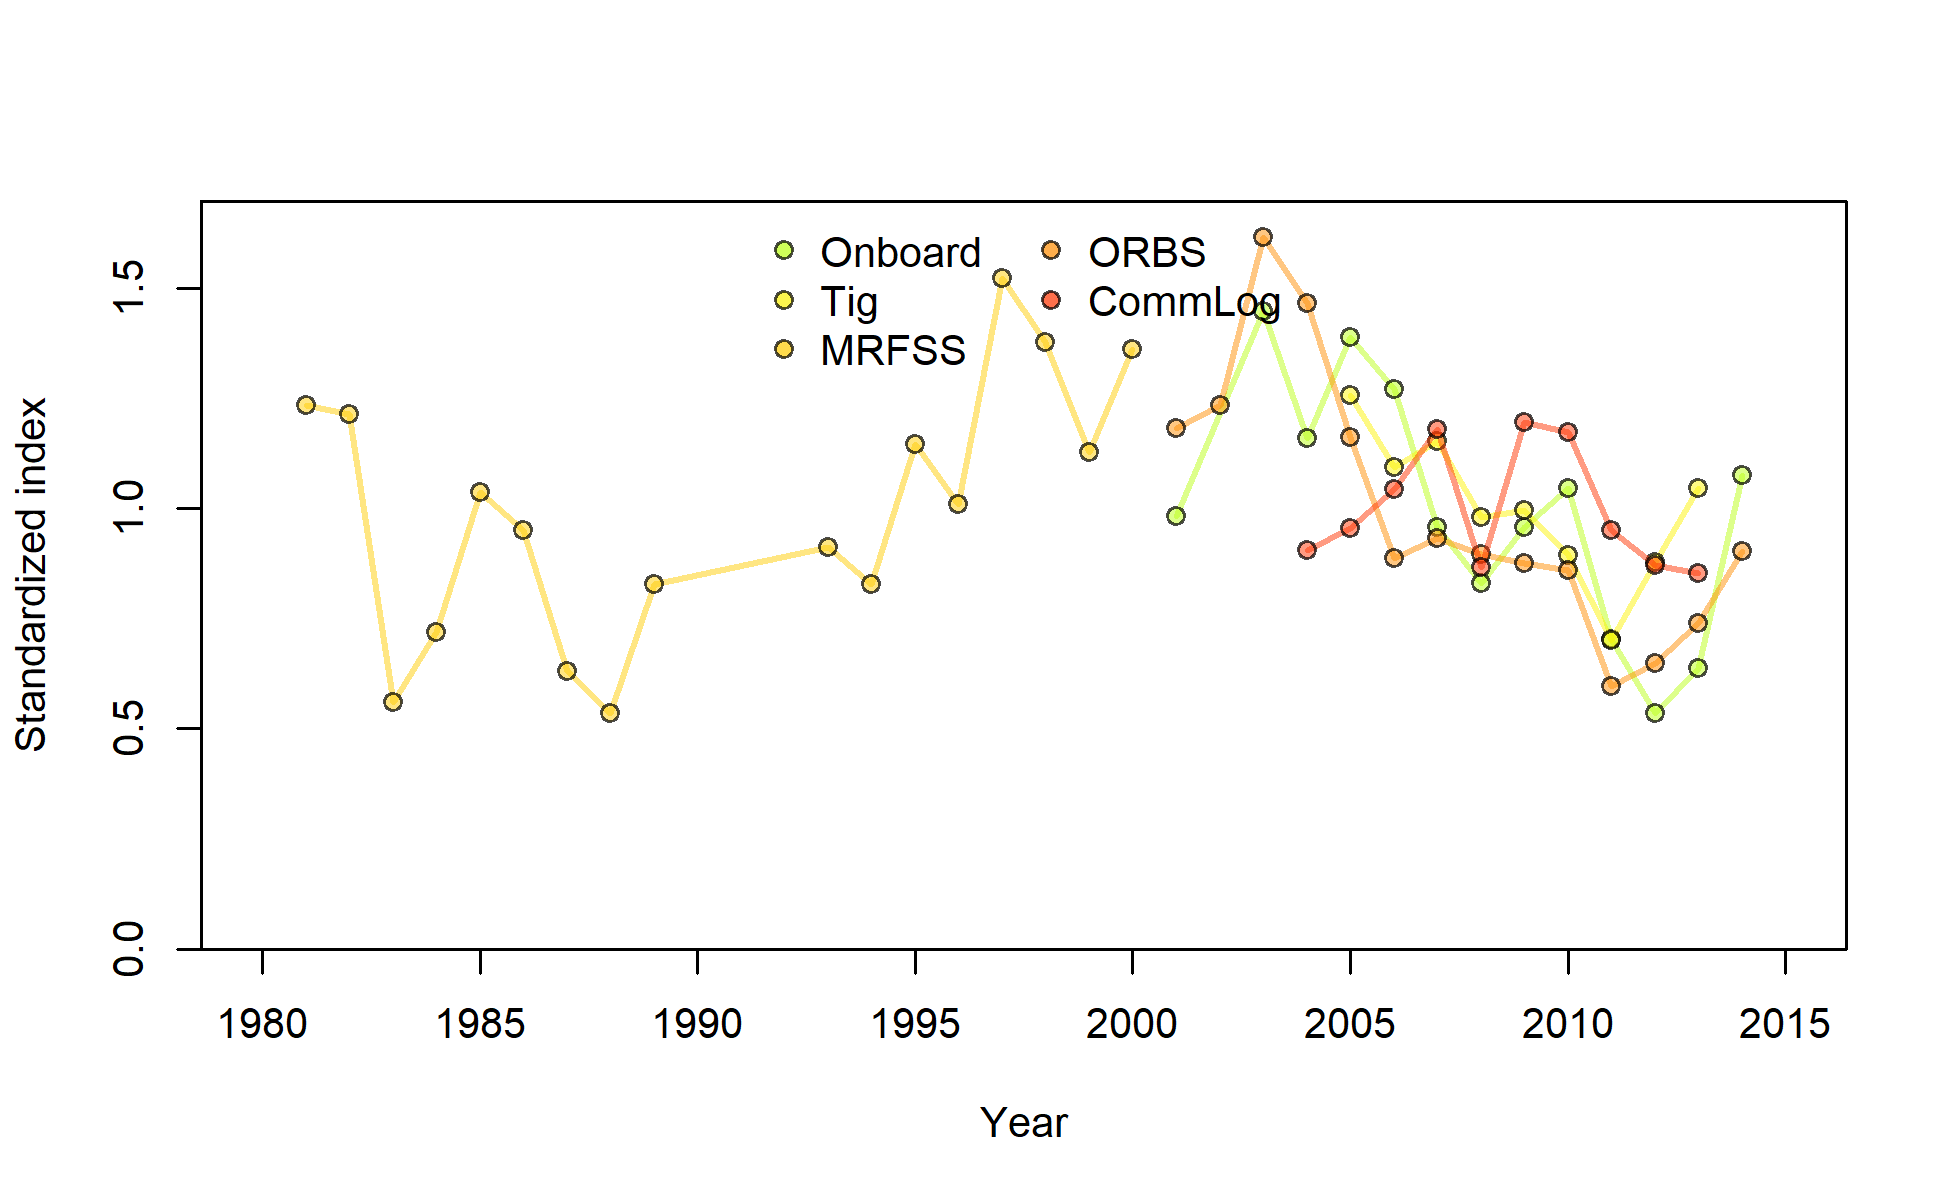
\includegraphics[width=1\textwidth,height=1\textheight]{C:/Users/Jason.Cope/Documents/Github/Sebastes_melanops_OR/Document/models/Reference model/plots/index9_standcpueall.png}
\caption{The set of standardized indices (each index is scaled to have a mean observation of 1) used in the base model.\label{fig:sur-summ-all}}
\end{figure}

\newpage

\begin{figure}
\centering
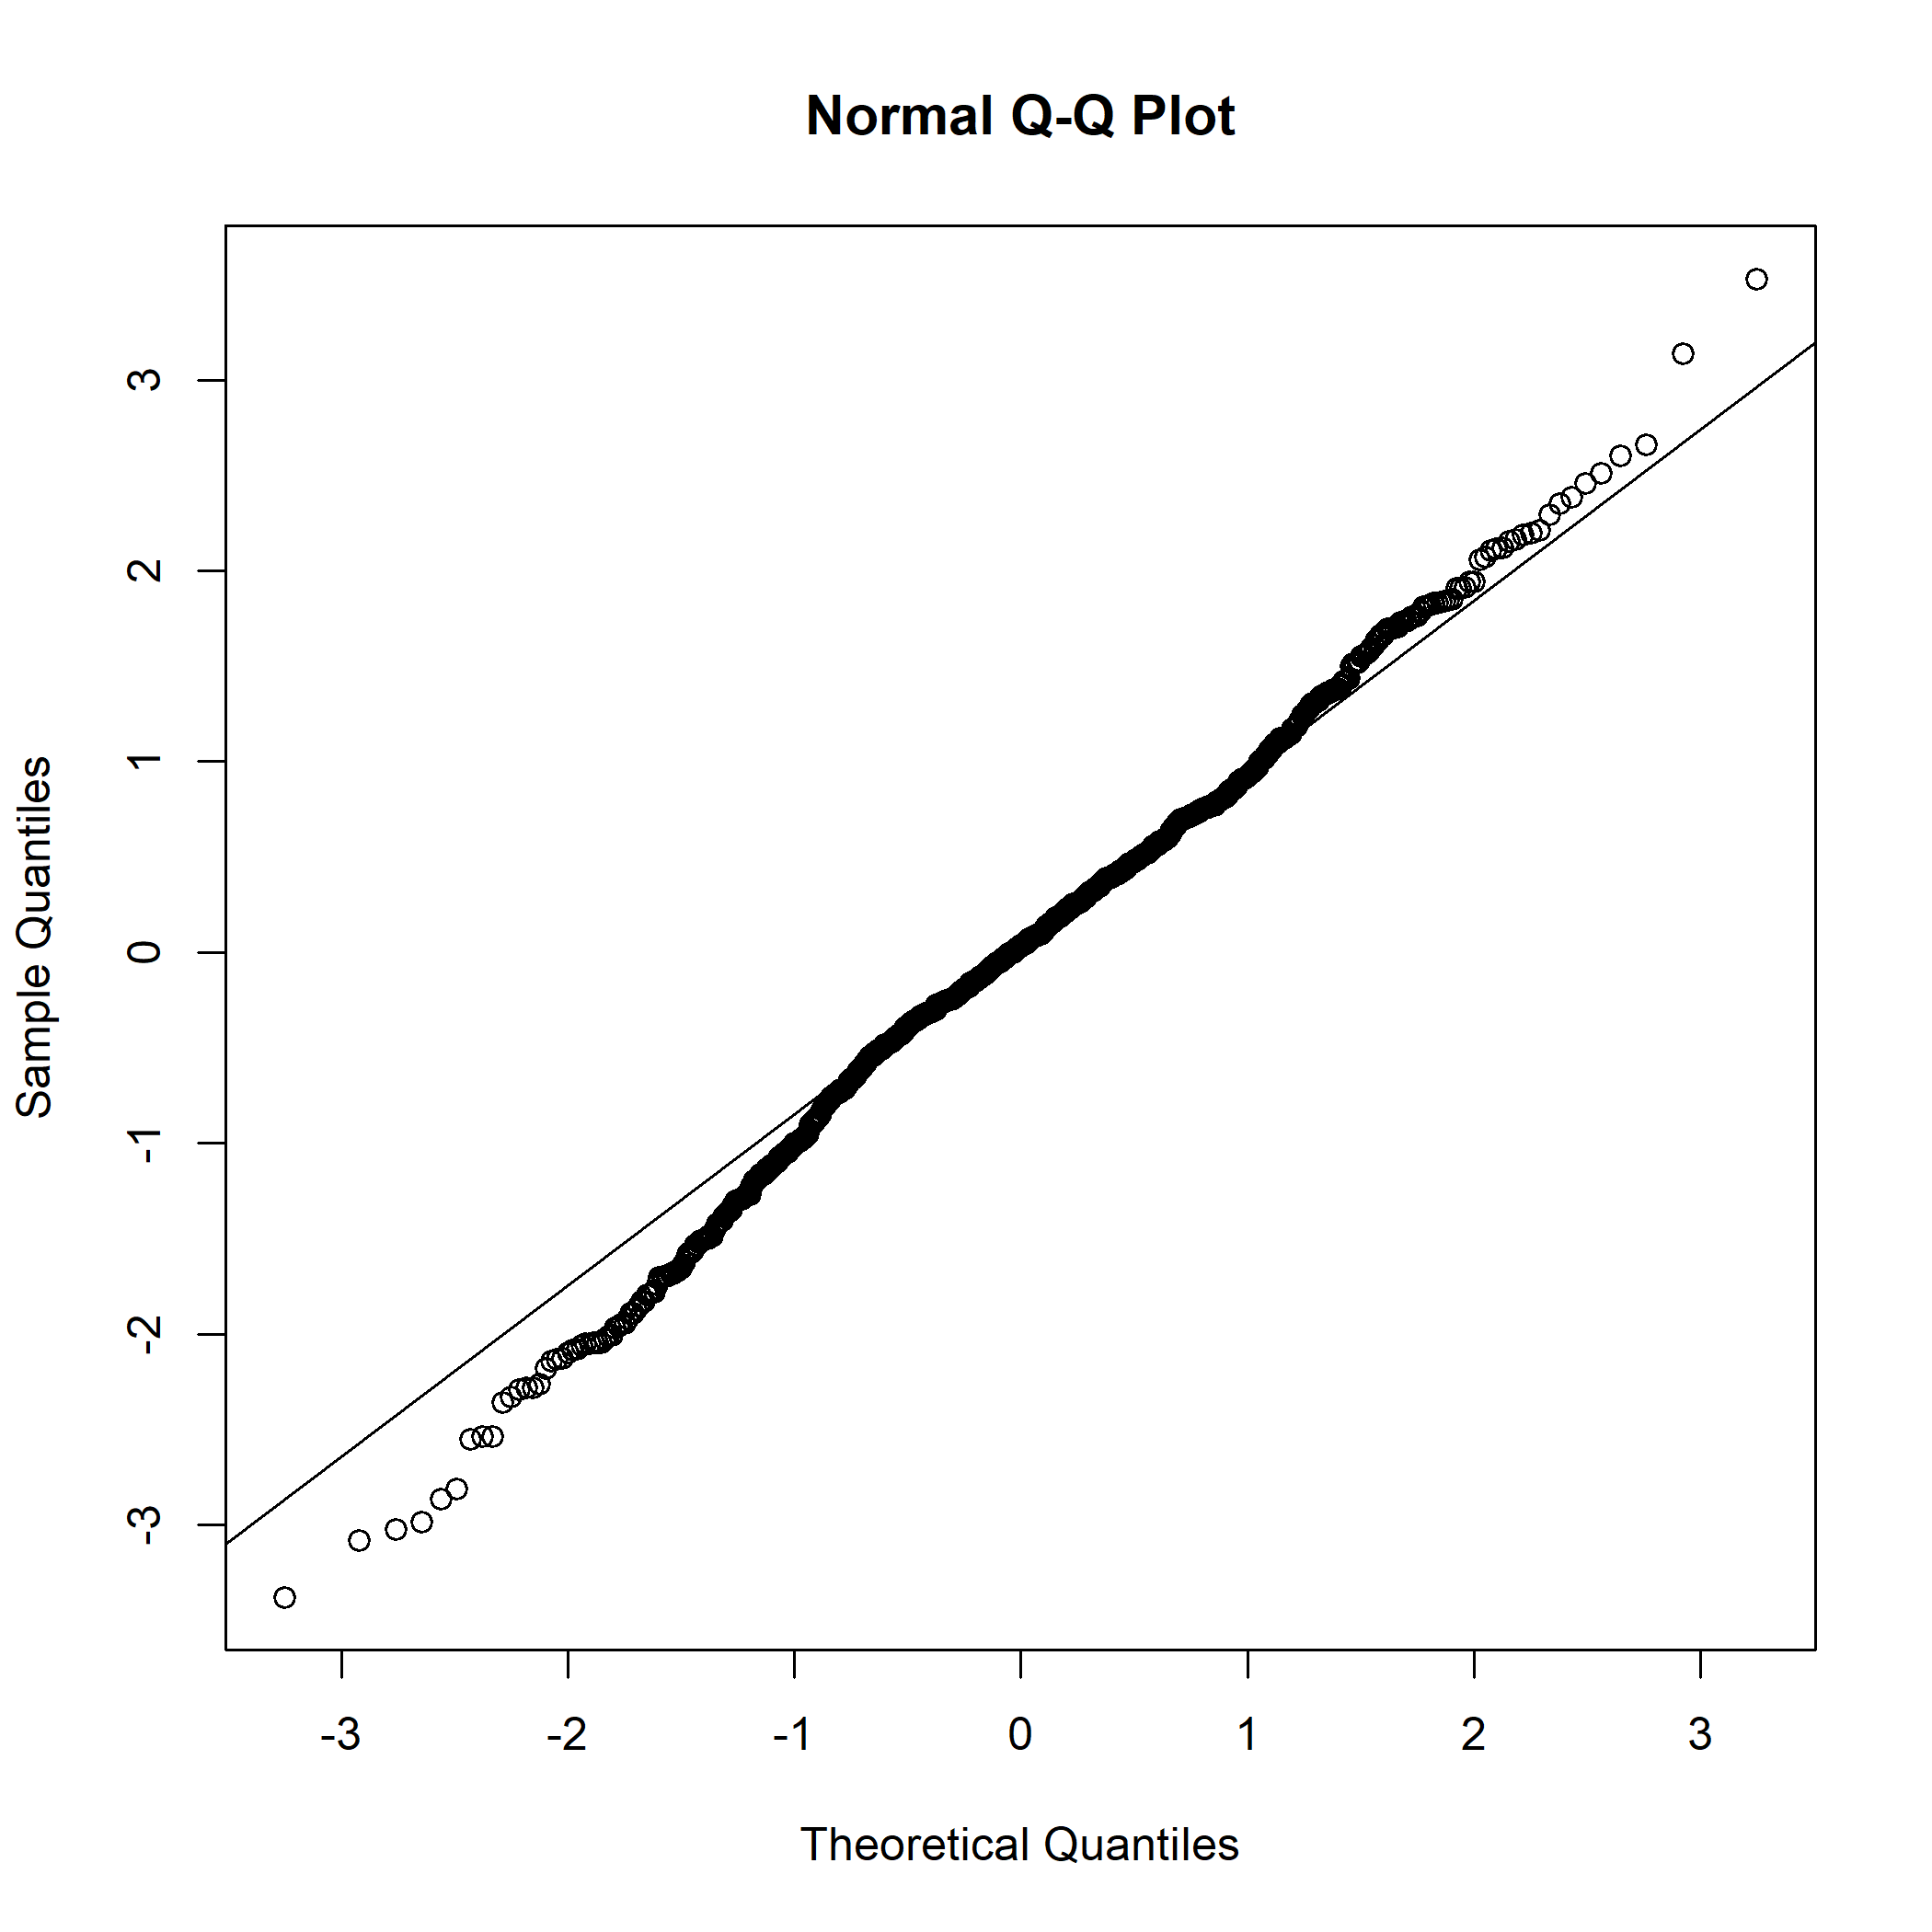
\includegraphics[width=1\textwidth,height=1\textheight]{C:/Users/Jason.Cope/Documents/Github/Sebastes_melanops_OR/Document/figures/index/qq_MRHnL.png}
\caption{Q-Q plot for the marine reserves hook and line survey.\label{fig:qq_MRHnL}}
\end{figure}

\newpage

\begin{figure}
\centering
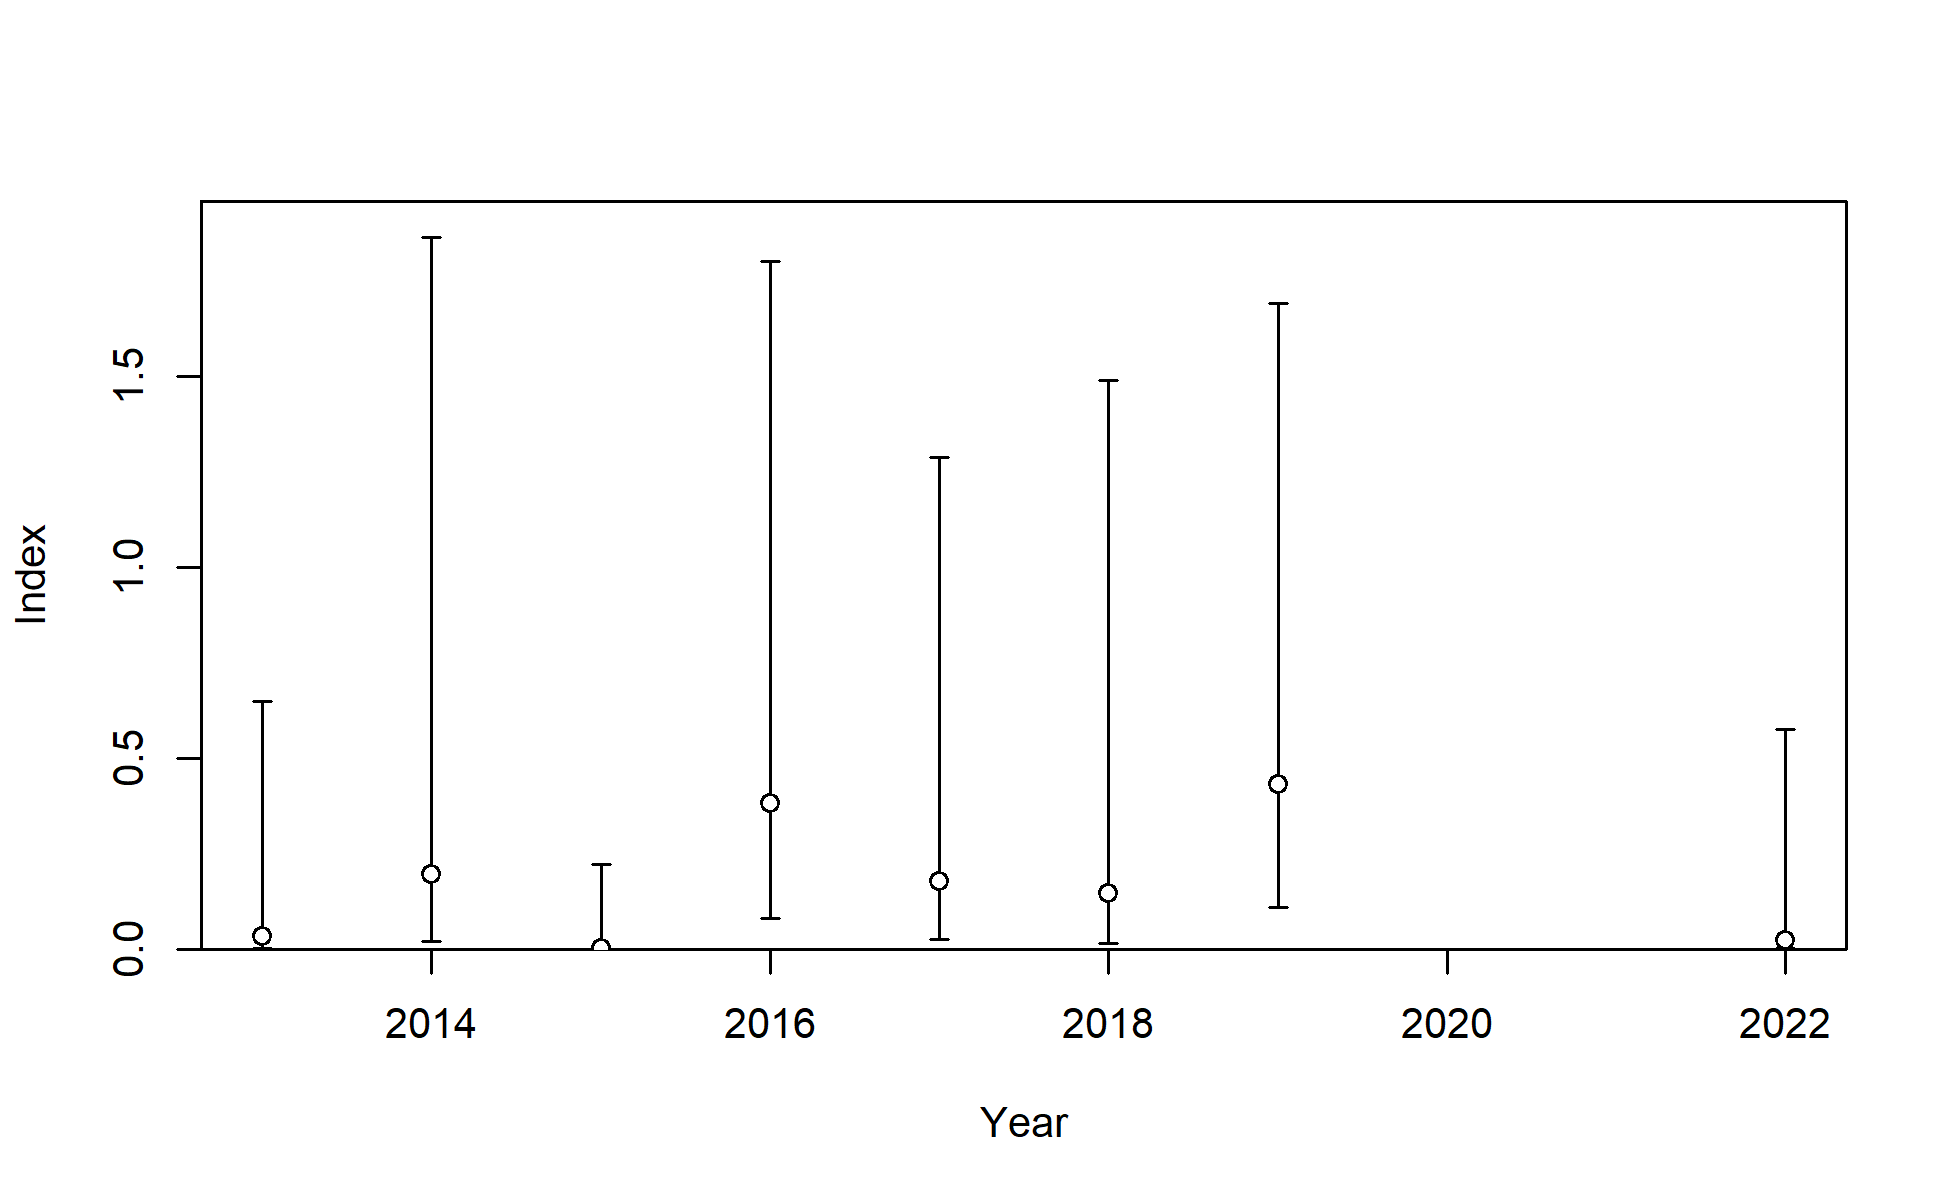
\includegraphics[width=1\textwidth,height=1\textheight]{C:/Users/Jason.Cope/Documents/Github/Sebastes_melanops_OR/Document/figures/index/index1_cpuedata_SMURF.png}
\caption{Index of recruitment from SMURF data collections. Error bars indicate 95\% uncertainty interval around index values based on the model assumption of lognormal error. This index was not included in the reference model, but was evaluated as a sensitivity.\label{fig:index1_cpuedata_SMURF}}
\end{figure}

\newpage

\hypertarget{model-results}{%
\subsection{Model Results}\label{model-results}}

\hypertarget{bridging}{%
\subsubsection{Bridging}\label{bridging}}

\begin{figure}
\centering
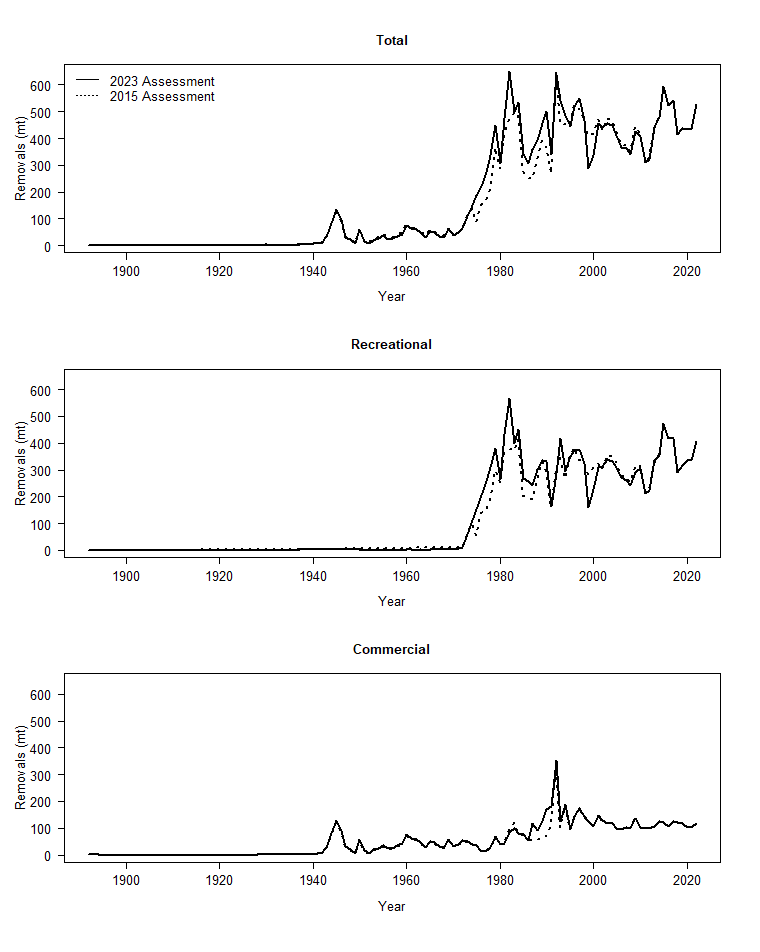
\includegraphics[width=1\textwidth,height=1\textheight]{C:/Users/Jason.Cope/Documents/Github/Sebastes_melanops_OR/Document/figures/Bridge/Assess_catch_compare.png}
\caption{Total (top panel), recreational (middle panel), and commercial (bottom panel) removal history used in this assessment compared to the previous (2015) assessment.\label{fig:catch-bridge}}
\end{figure}

\newpage

\begin{figure}
\centering
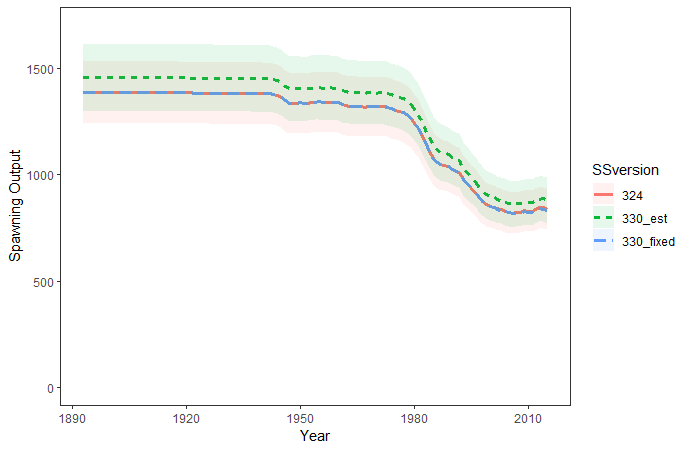
\includegraphics[width=1\textwidth,height=1\textheight]{C:/Users/Jason.Cope/Documents/Github/Sebastes_melanops_OR/Document/figures/Bridge/OR_SB_comp_plot.png}
\caption{Comparison of spawning output for black rockfish in waters off of Oregon between Stock Synthesis versions 3.24 and 3.30. Uncertainty envelops are 95\% confidence intervals.\label{fig:ssb-bridge-comps}}
\end{figure}

\newpage

\begin{figure}
\centering
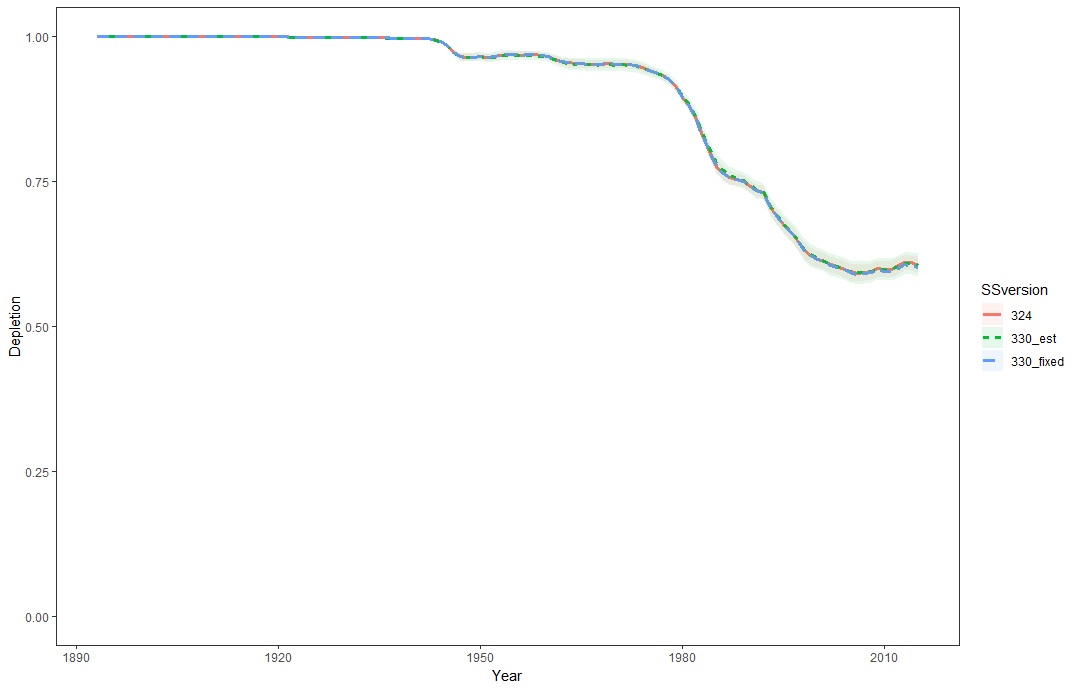
\includegraphics[width=1\textwidth,height=1\textheight]{C:/Users/Jason.Cope/Documents/Github/Sebastes_melanops_OR/Document/figures/Bridge/OR_Dep_comp_plot.png}
\caption{Comparison of spawning output for black rockfish in waters off of Oregon between Stock Synthesis versions 3.24 and 3.30. Uncertainty envelops are 95\% confidence intervals.\label{fig:deps-bridge-comps}}
\end{figure}

\clearpage

\hypertarget{model-development}{%
\subsubsection{Model Development}\label{model-development}}

\begin{figure}
\centering
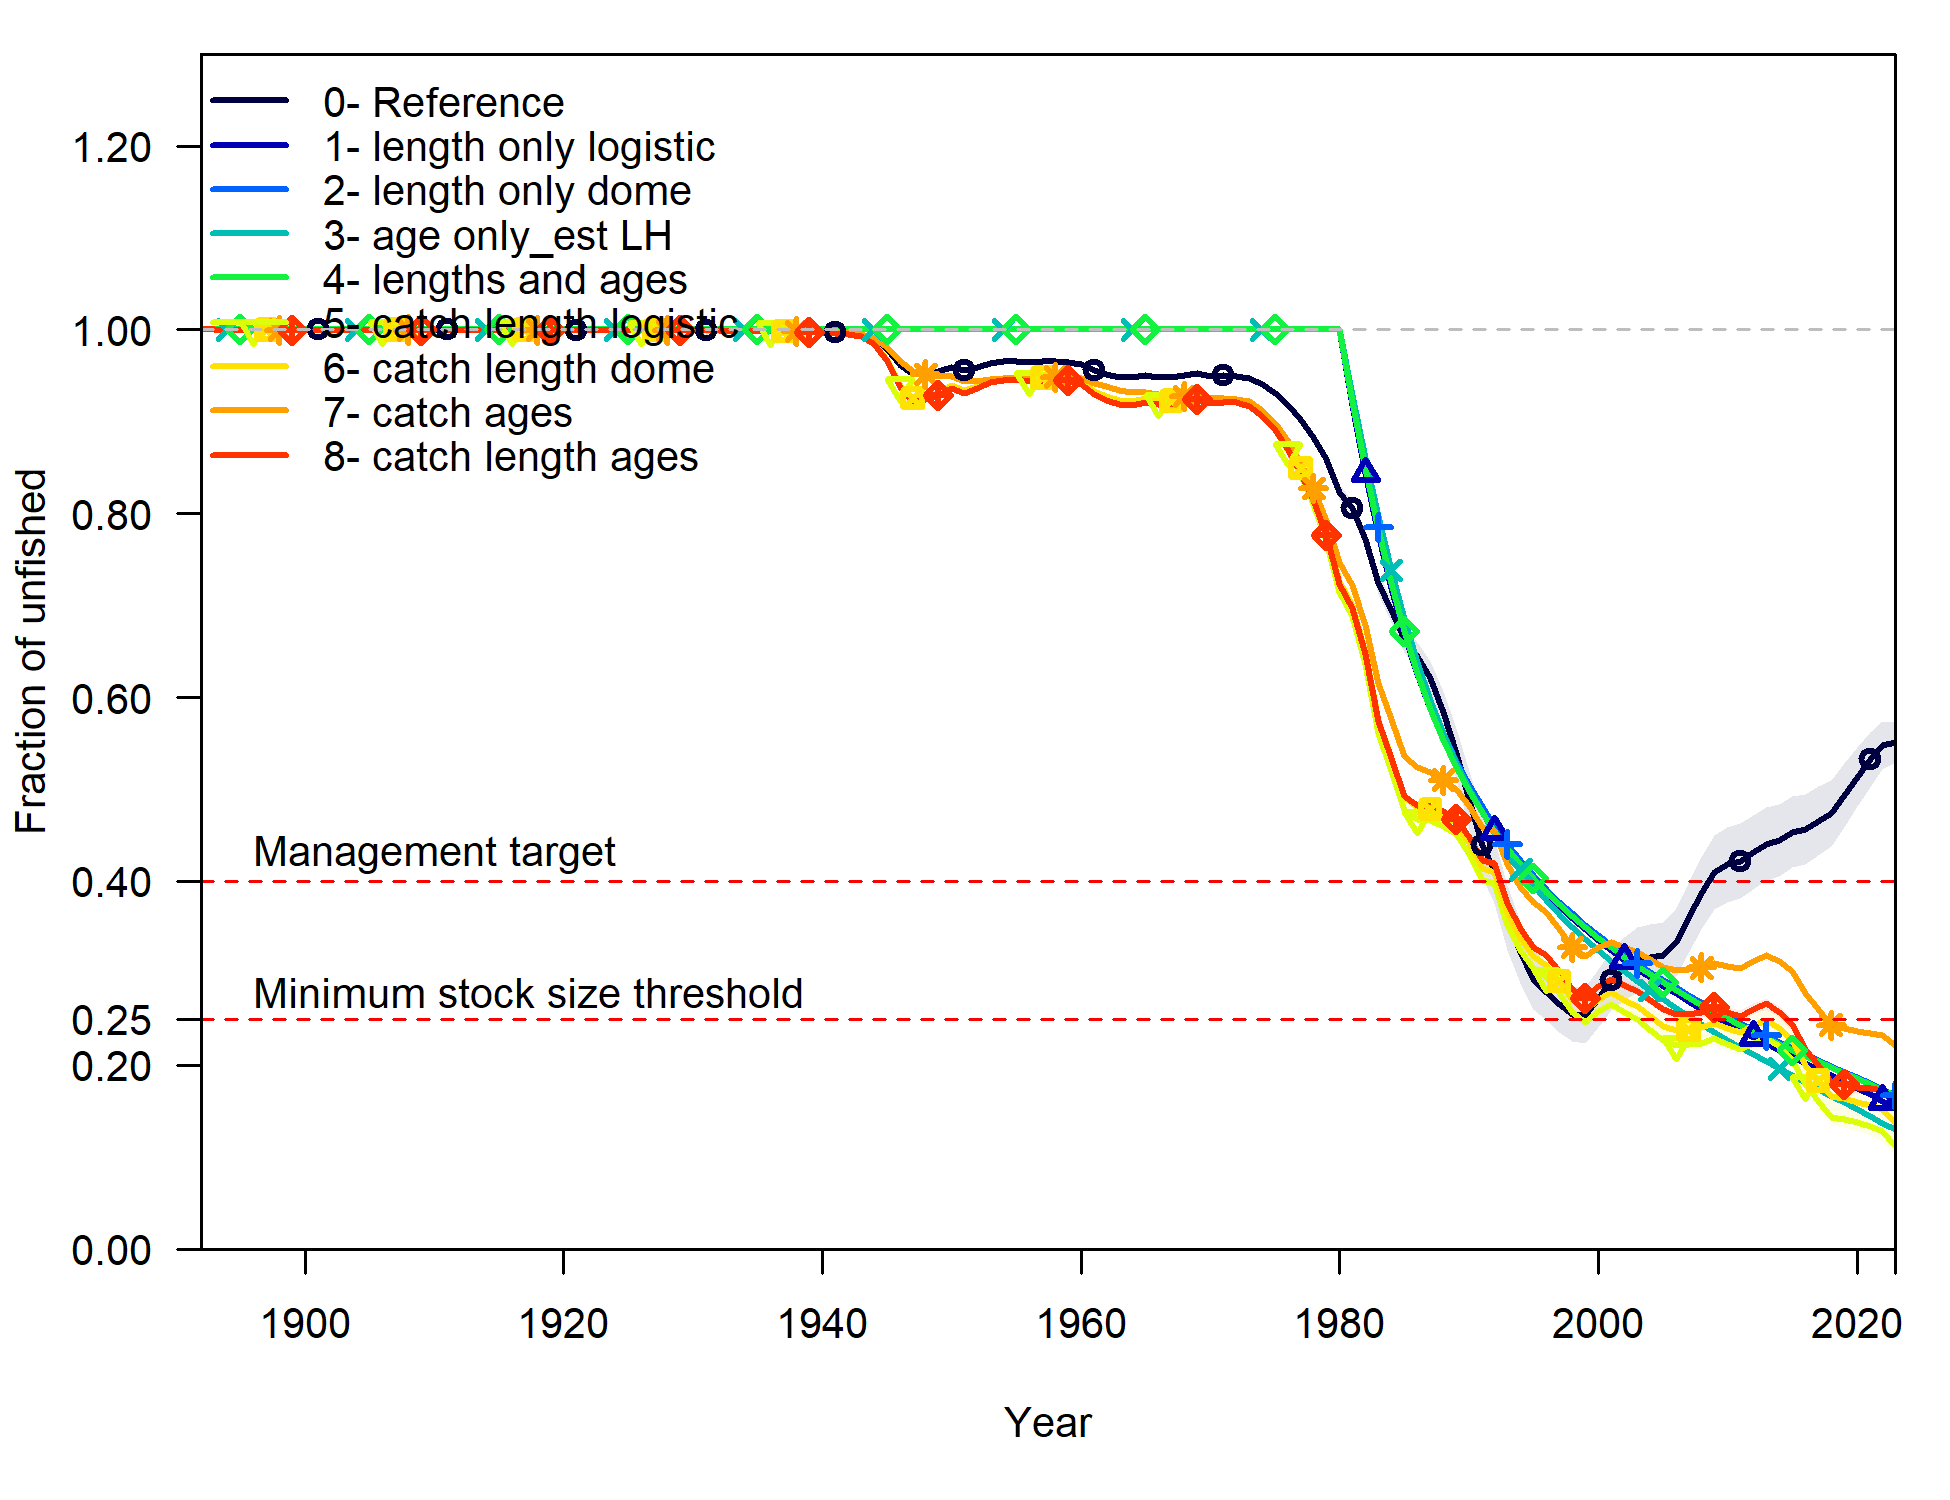
\includegraphics[width=1\textwidth,height=1\textheight]{C:/Users/Jason.Cope/Documents/Github/Sebastes_melanops_OR/Document/figures/modbuild/Mod build stock status/compare4_Bratio_uncertainty.png}
\caption{Relative spawning output time series by data treatment compared to the reference model. Missing scenarios mean the spawning output was too large to show.\label{fig:modbuild-data-depl}}
\end{figure}

\newpage

\begin{figure}
\centering
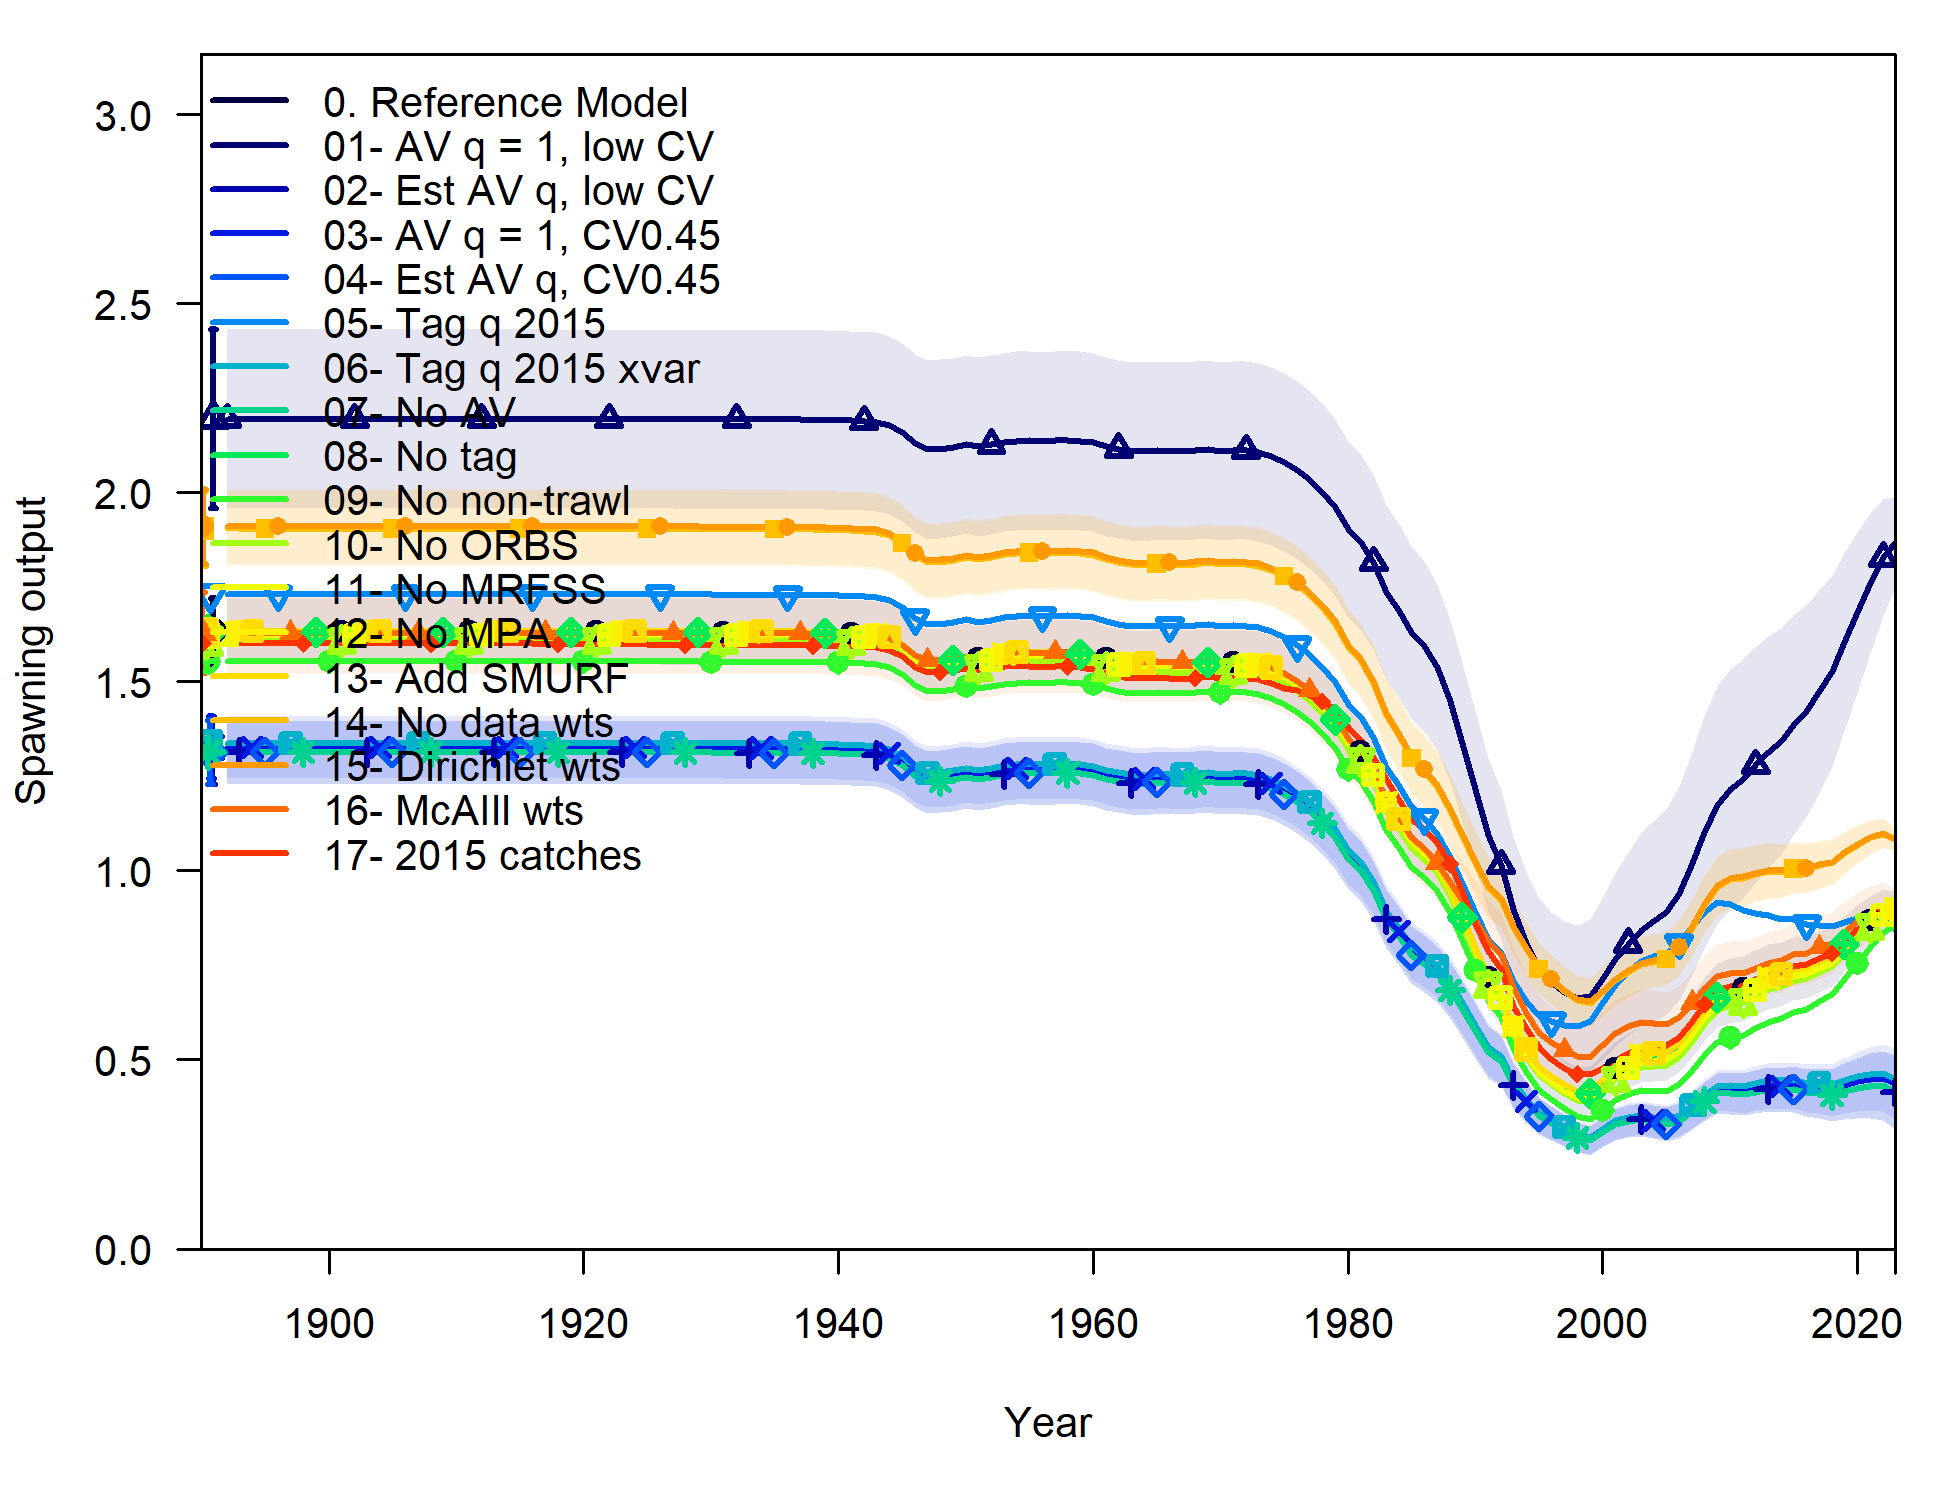
\includegraphics[width=1\textwidth,height=1\textheight]{C:/Users/Jason.Cope/Documents/Github/Sebastes_melanops_OR/Document/figures/modbuild/Mod build stock scale/compare2_spawnbio_uncertainty.png}
\caption{Spawning output (in millions of eggs) time series by data treatment compared to the reference model.\label{fig:modbuild-data-ssb}}
\end{figure}

\newpage

\begin{figure}
\centering
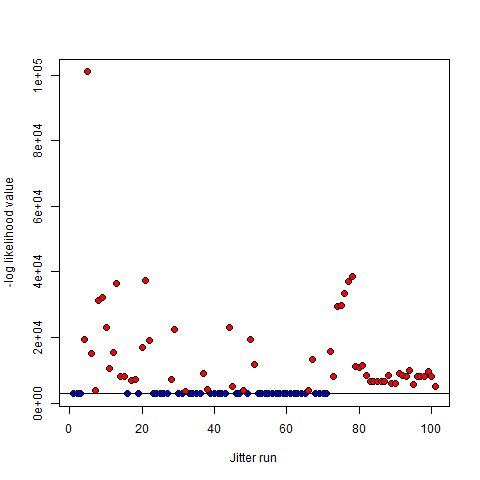
\includegraphics[width=1\textwidth,height=1\textheight]{C:/Users/Jason.Cope/Documents/Github/Sebastes_melanops_OR/Document/figures/modconverge/jitterplot.png}
\caption{Jitter runs for the black rockfish reference model, with jitter run number on the x-axis and -log likelihood value on the y-axis. Blue dot are models that match the likelihood value of the reference model, while red dots deviate from the reference model. All red dots are above the blue dots, indicating no better fit to the reference model was found.\label{fig:jitter}}
\end{figure}

\newpage

\begin{figure}
\centering
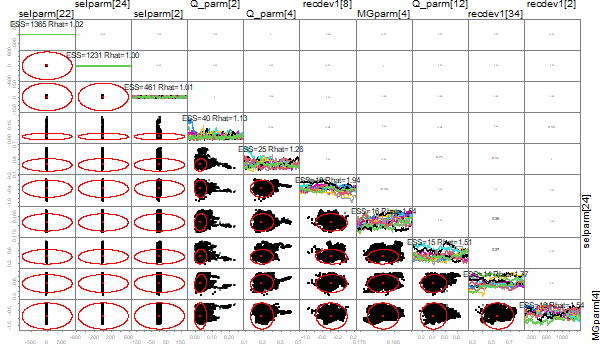
\includegraphics[width=1\textwidth,height=1\textheight]{C:/Users/Jason.Cope/Documents/Github/Sebastes_melanops_OR/Document/figures/modconverge/pairs_plot_fast.png}
\caption{Pairs plots of the fastest mixing parameters from running 2000 posterior draws (and keep every draw) using the random walk Metropolis algorithm. Parameters that show little to no movement are recommended to be fixed to improve model speed and efficiency.\label{fig:pairs-plot-fast}}
\end{figure}

\clearpage

\hypertarget{fit-to-data}{%
\subsubsection{Fit to Data}\label{fit-to-data}}

\begin{figure}
\centering
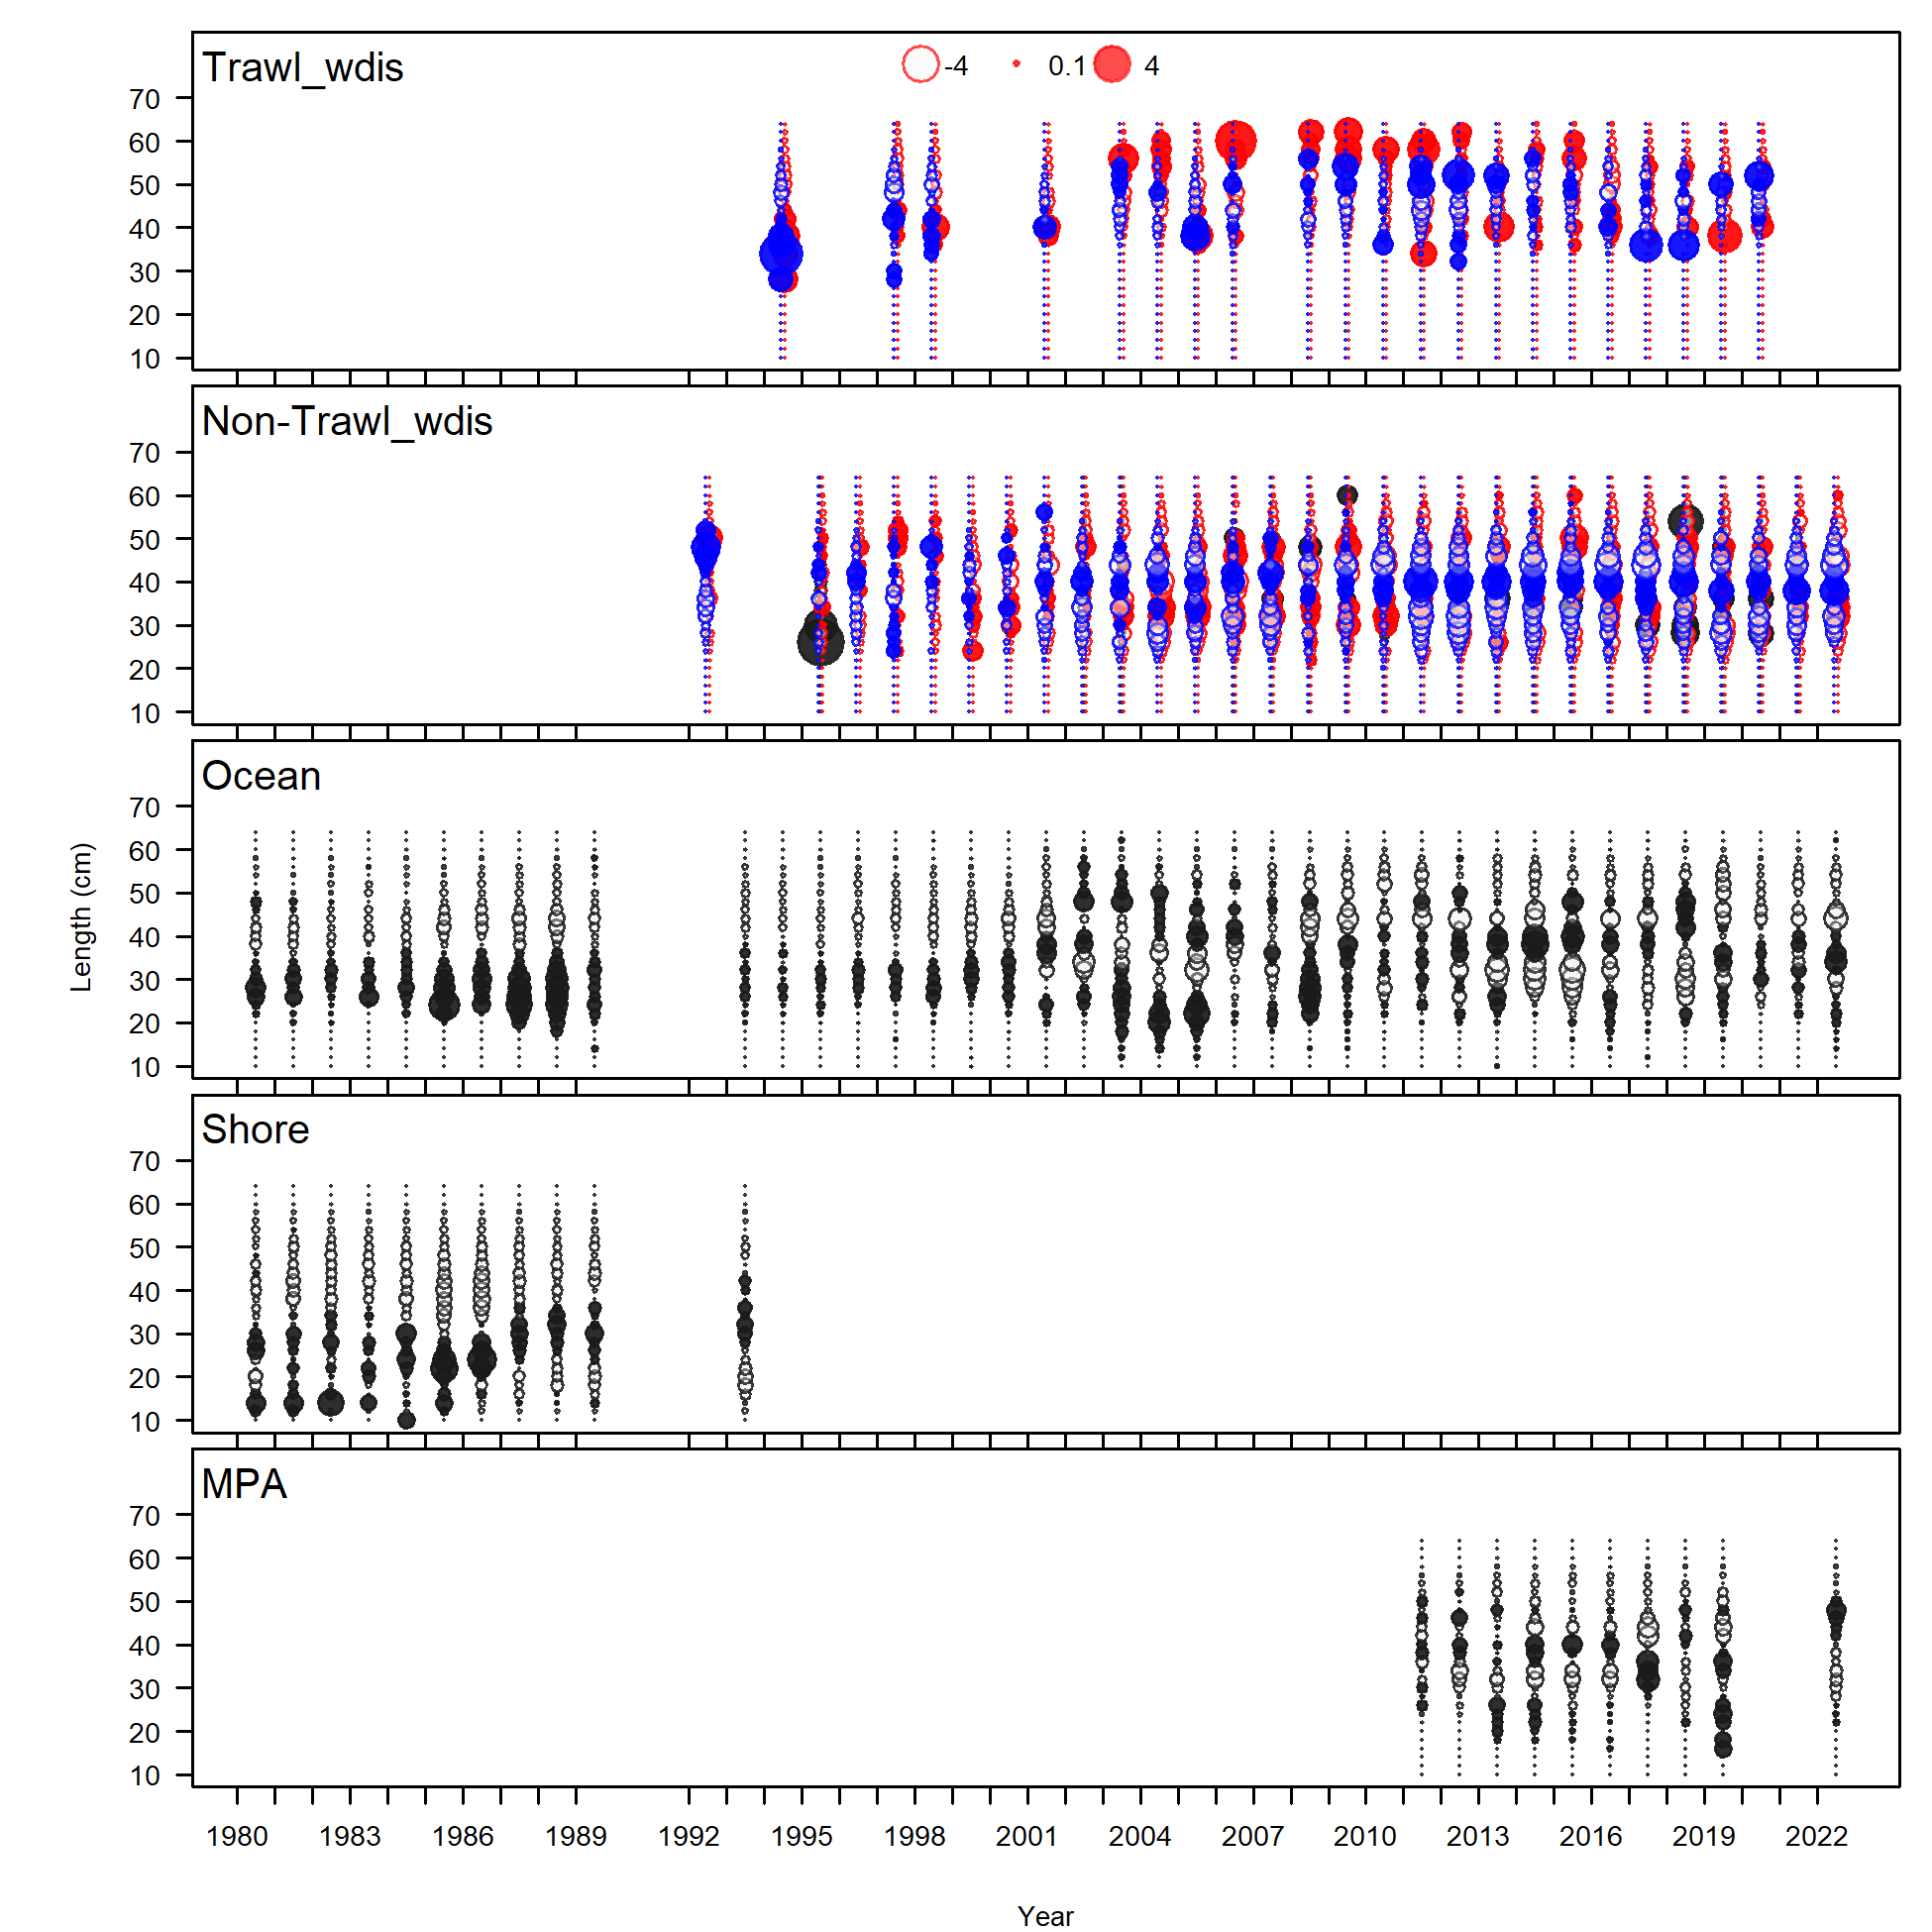
\includegraphics[width=1\textwidth,height=1\textheight]{C:/Users/Jason.Cope/Documents/Github/Sebastes_melanops_OR/Document/models/Reference model/plots/comp_lenfit__multi-fleet_comparison.png}
\caption{Pearson residuals for each fishing fleet and the MPA survey. Closed bubble are positive residuals (observed \textgreater{} expected) and open bubbles are negative residuals (observed \textless{} expected).\label{fig:lt-pearson-resids}}
\end{figure}

\newpage

\begin{figure}
\centering
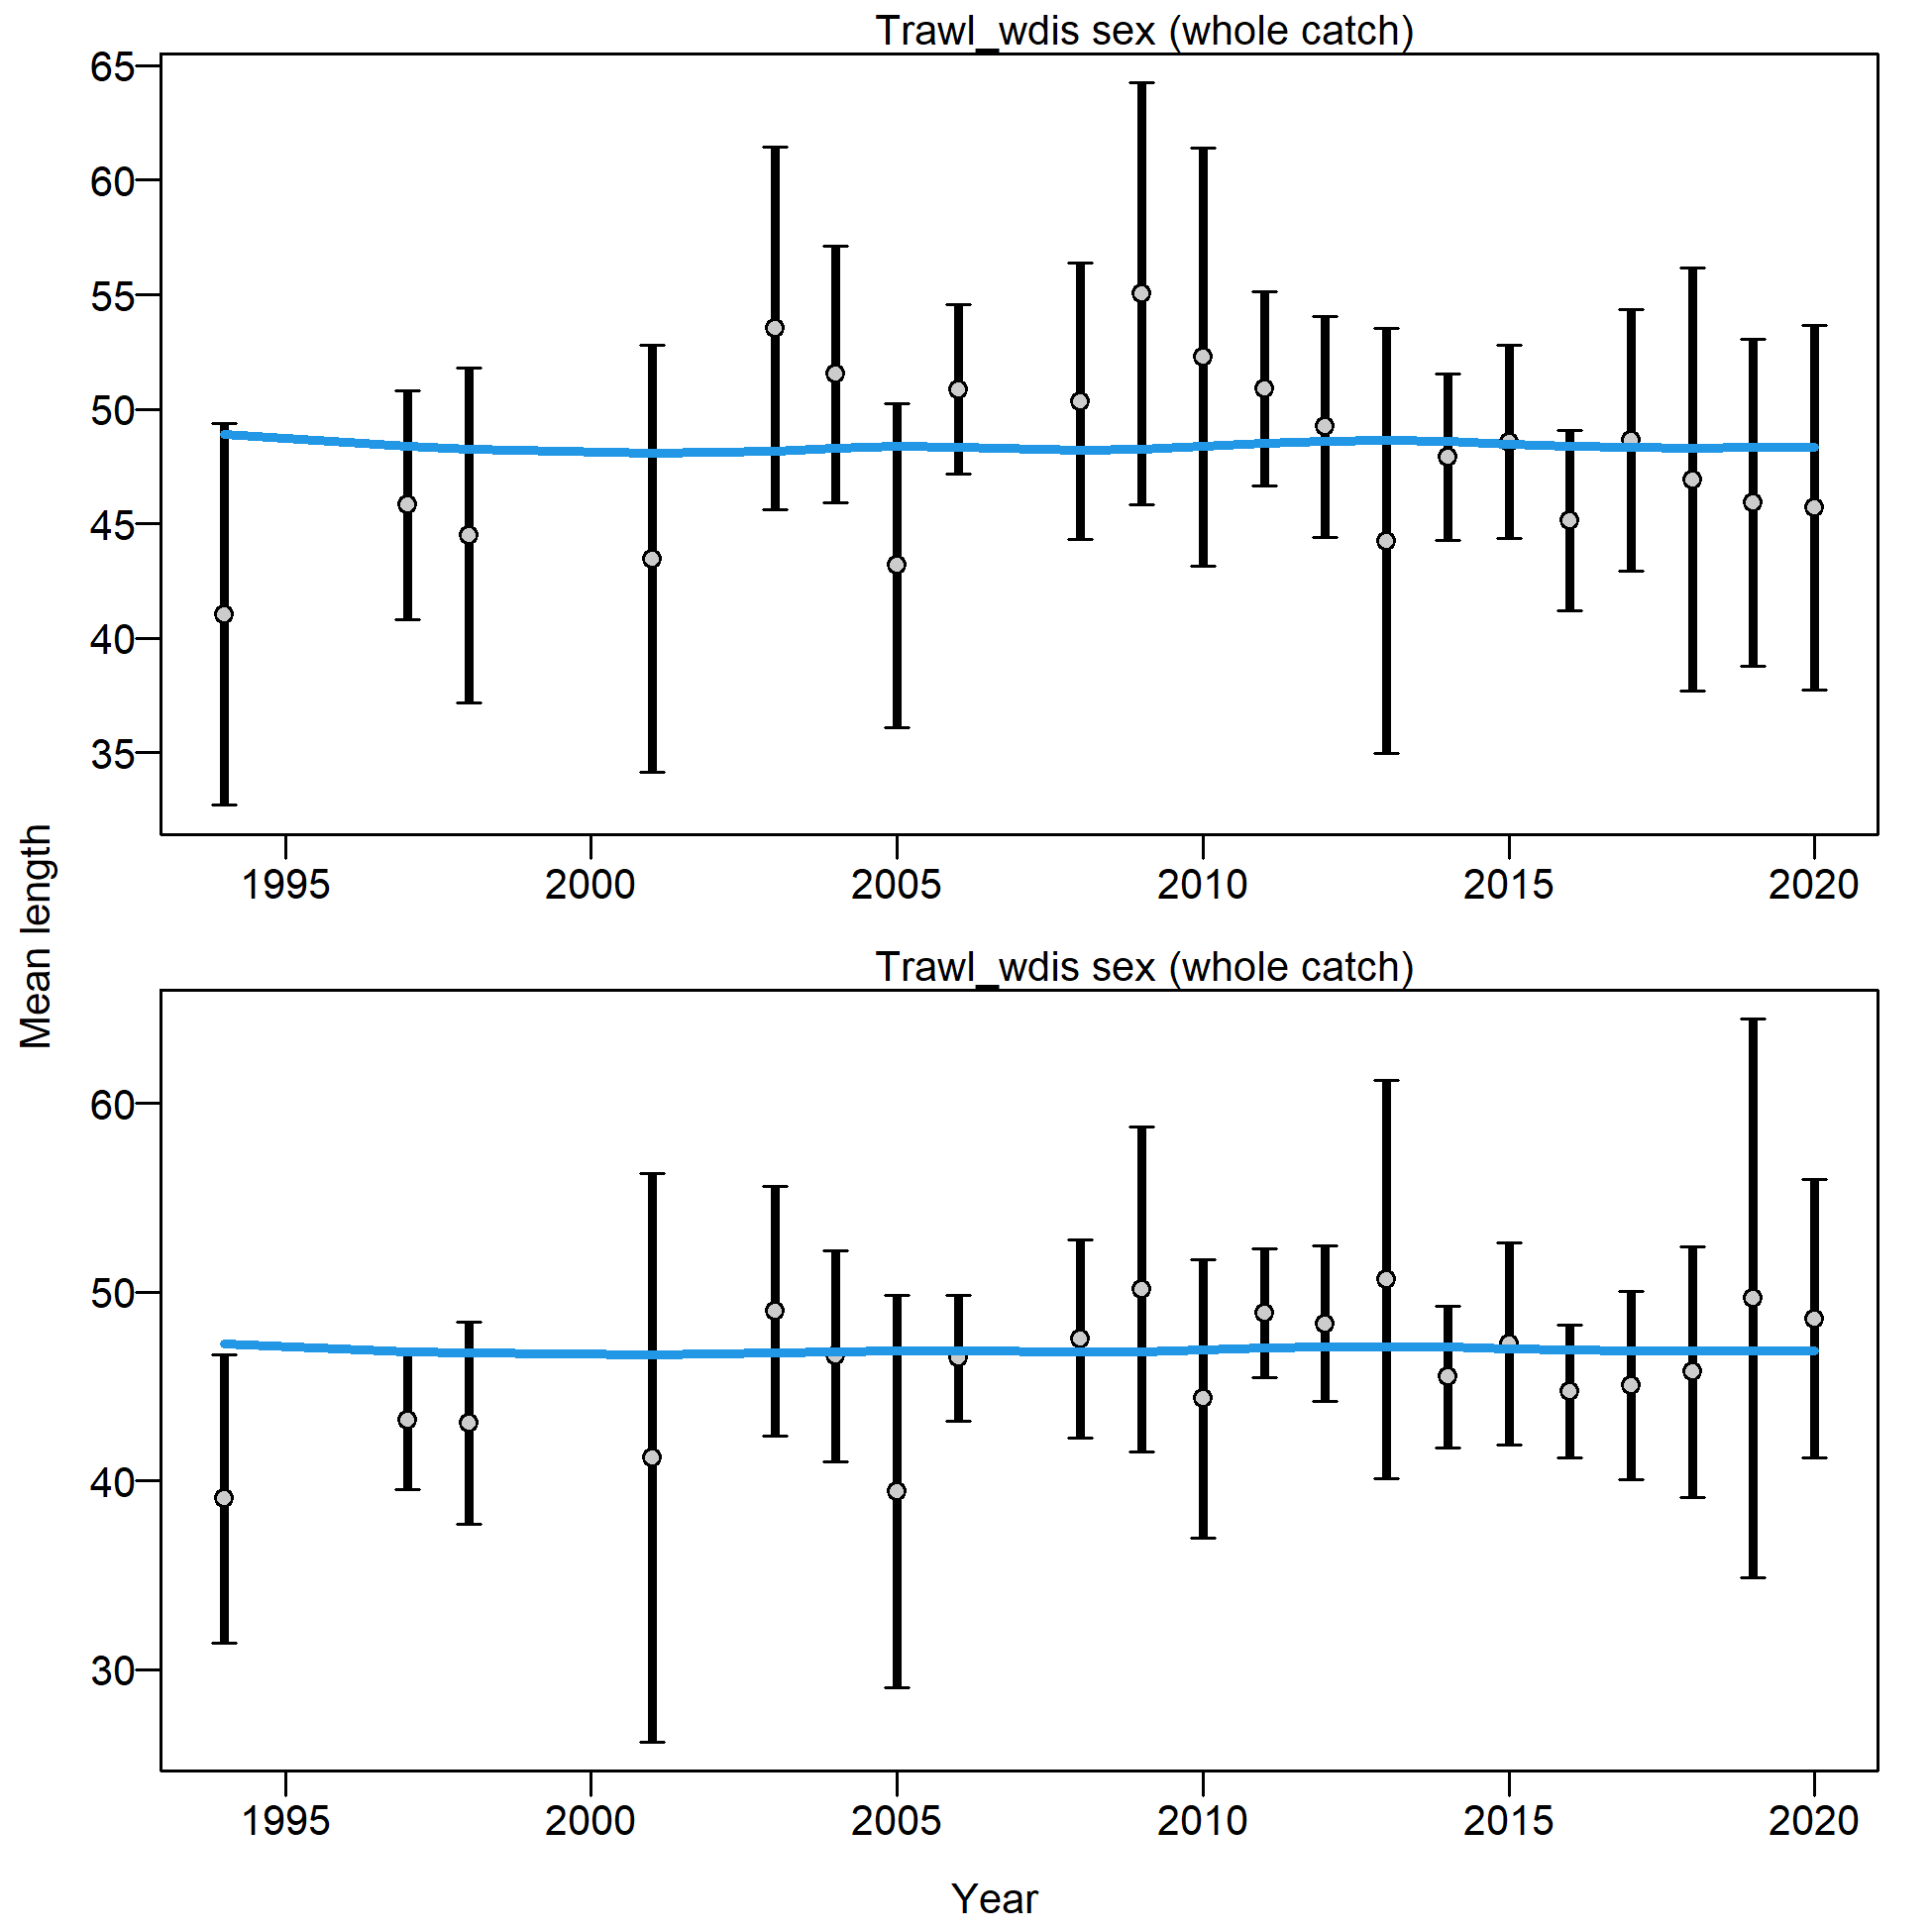
\includegraphics[width=1\textwidth,height=1\textheight]{C:/Users/Jason.Cope/Documents/Github/Sebastes_melanops_OR/Document/models/Reference model/plots/comp_lenfit_data_weighting_TA1.8_Trawl_wdis.png}
\caption{Mean length (cm) index from the commercial trawl fishery with 95 percent confidence intervals based on sample sizes and data weighting.\label{fig:trawl-mean-len-fit}}
\end{figure}

\newpage

\begin{figure}
\centering
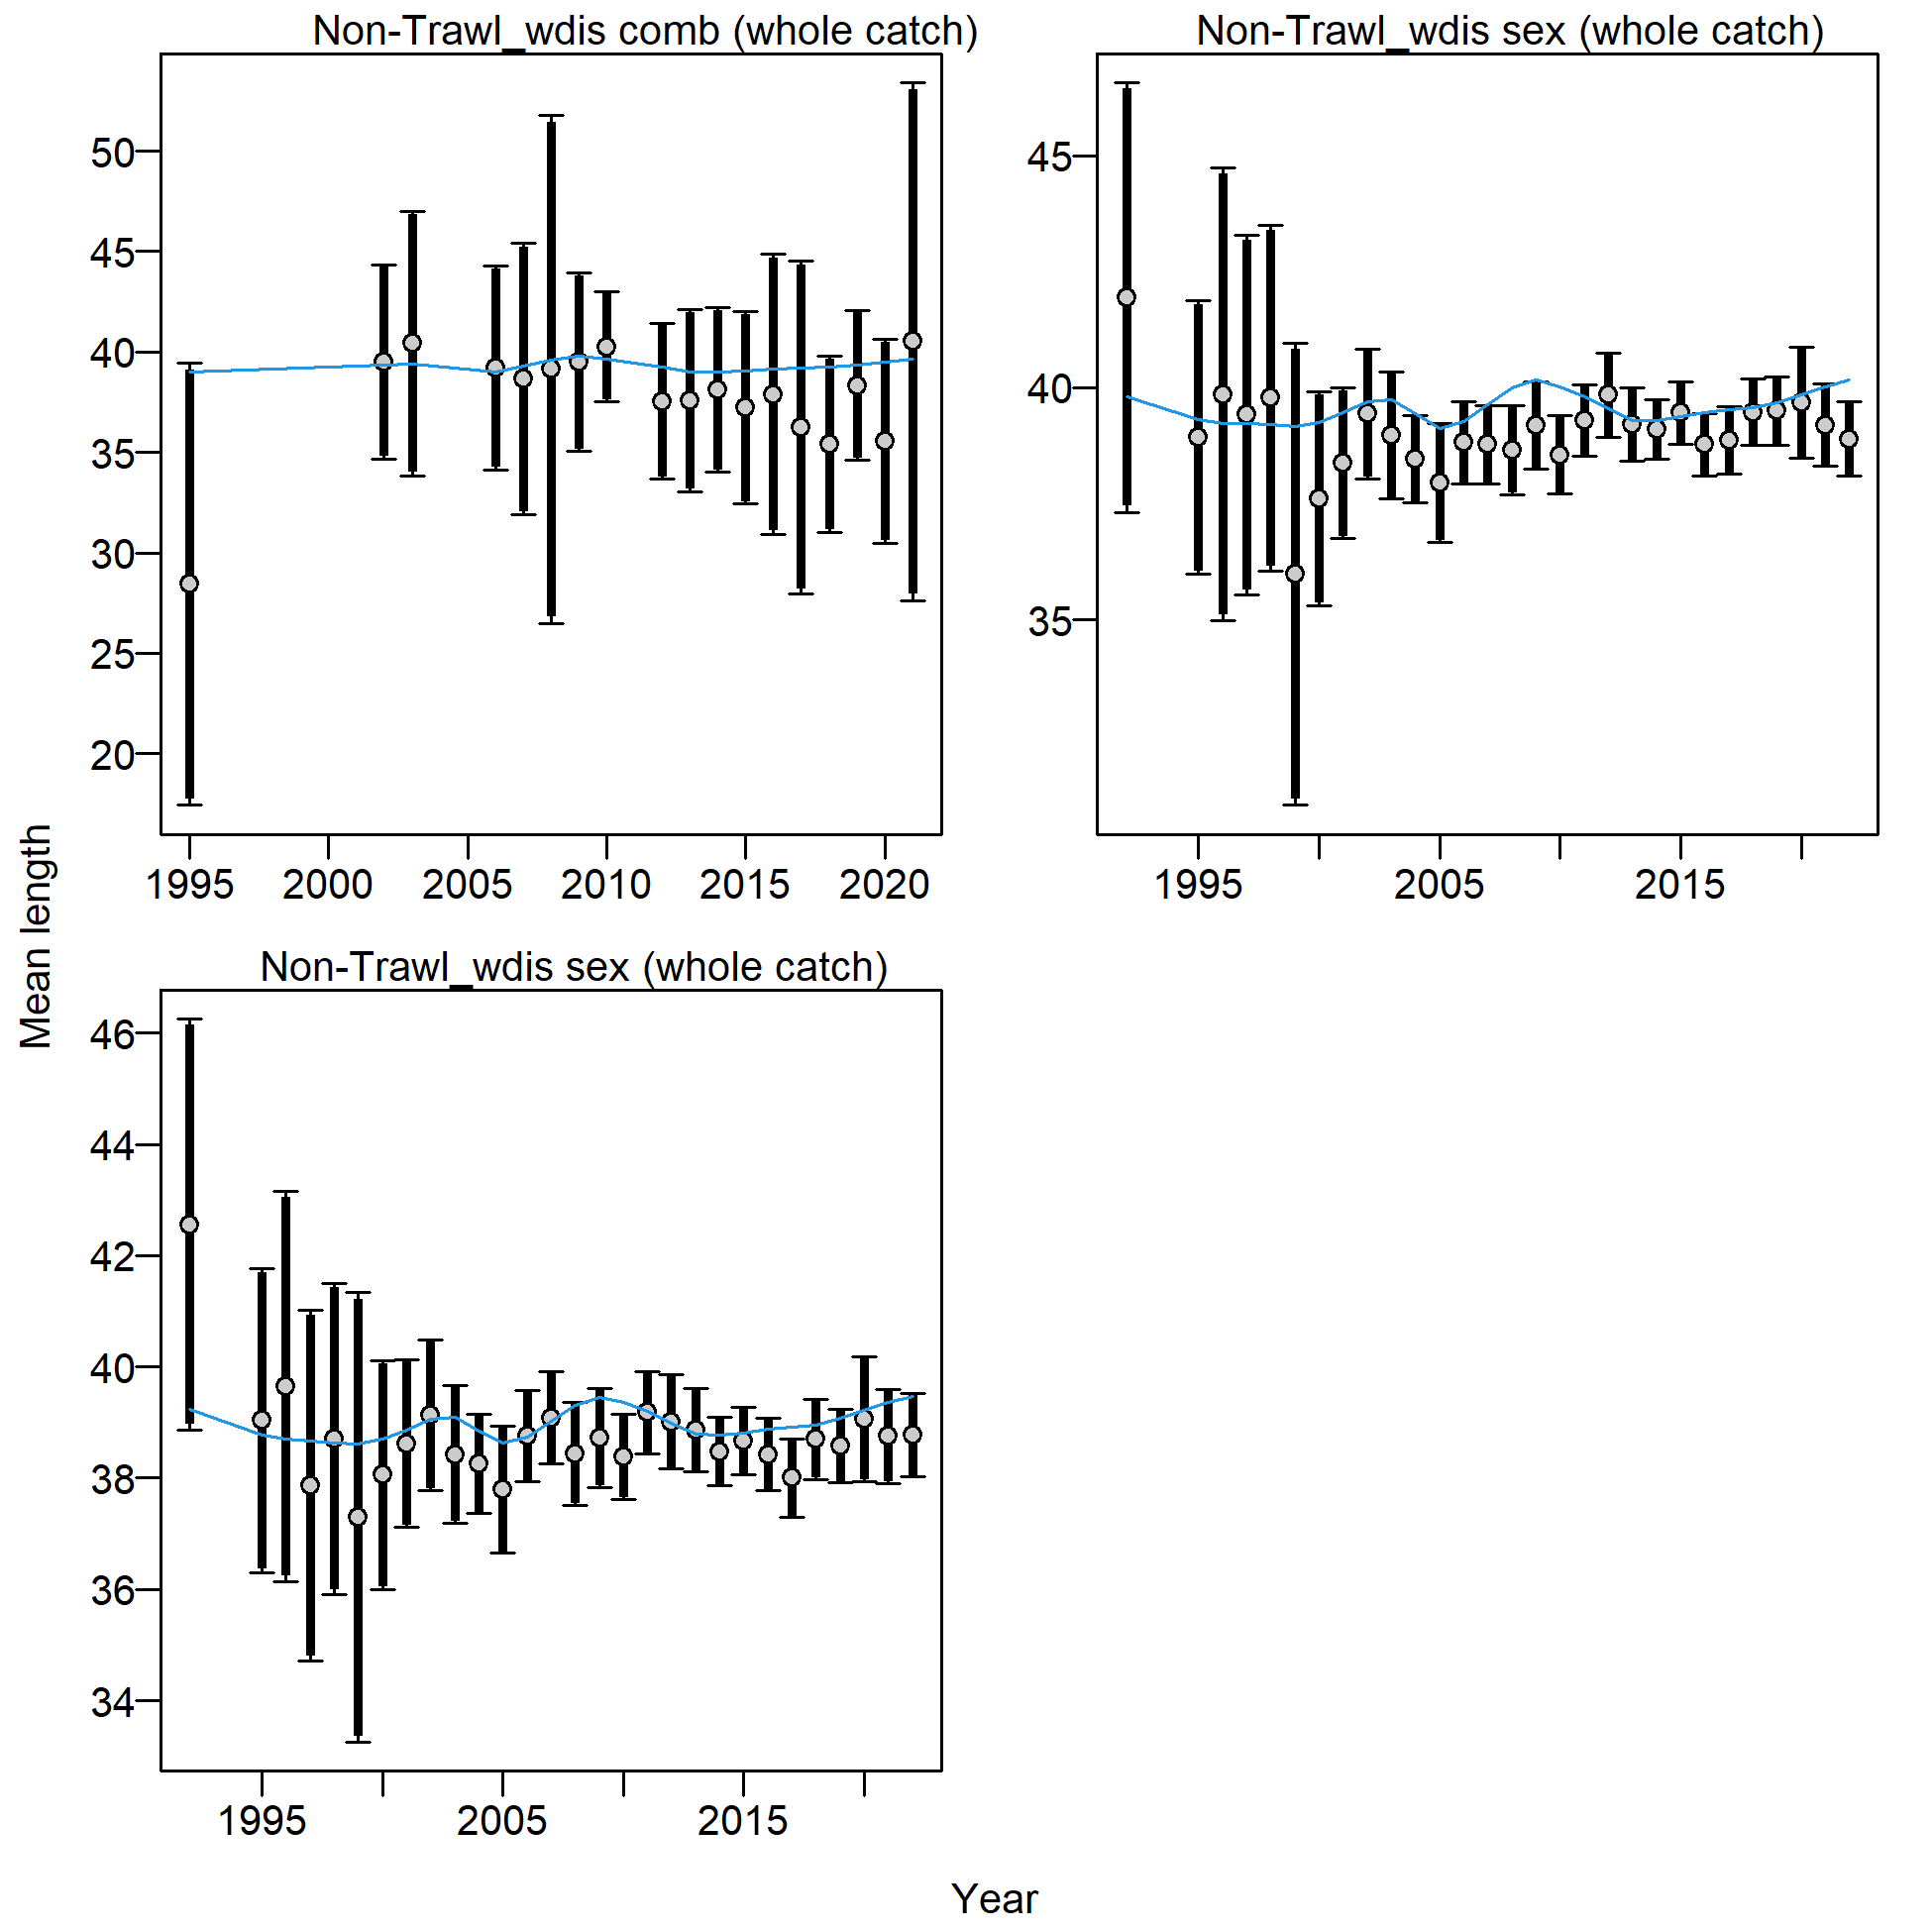
\includegraphics[width=1\textwidth,height=1\textheight]{C:/Users/Jason.Cope/Documents/Github/Sebastes_melanops_OR/Document/models/Reference model/plots/comp_lenfit_data_weighting_TA1.8_Non-Trawl_wdis.png}
\caption{Mean length (cm) index from the commercial non-trawl fishery with 95 percent confidence intervals based on sample sizes and data weighting.\label{fig:nontrawl-mean-len-fit}}
\end{figure}

\newpage

\begin{figure}
\centering
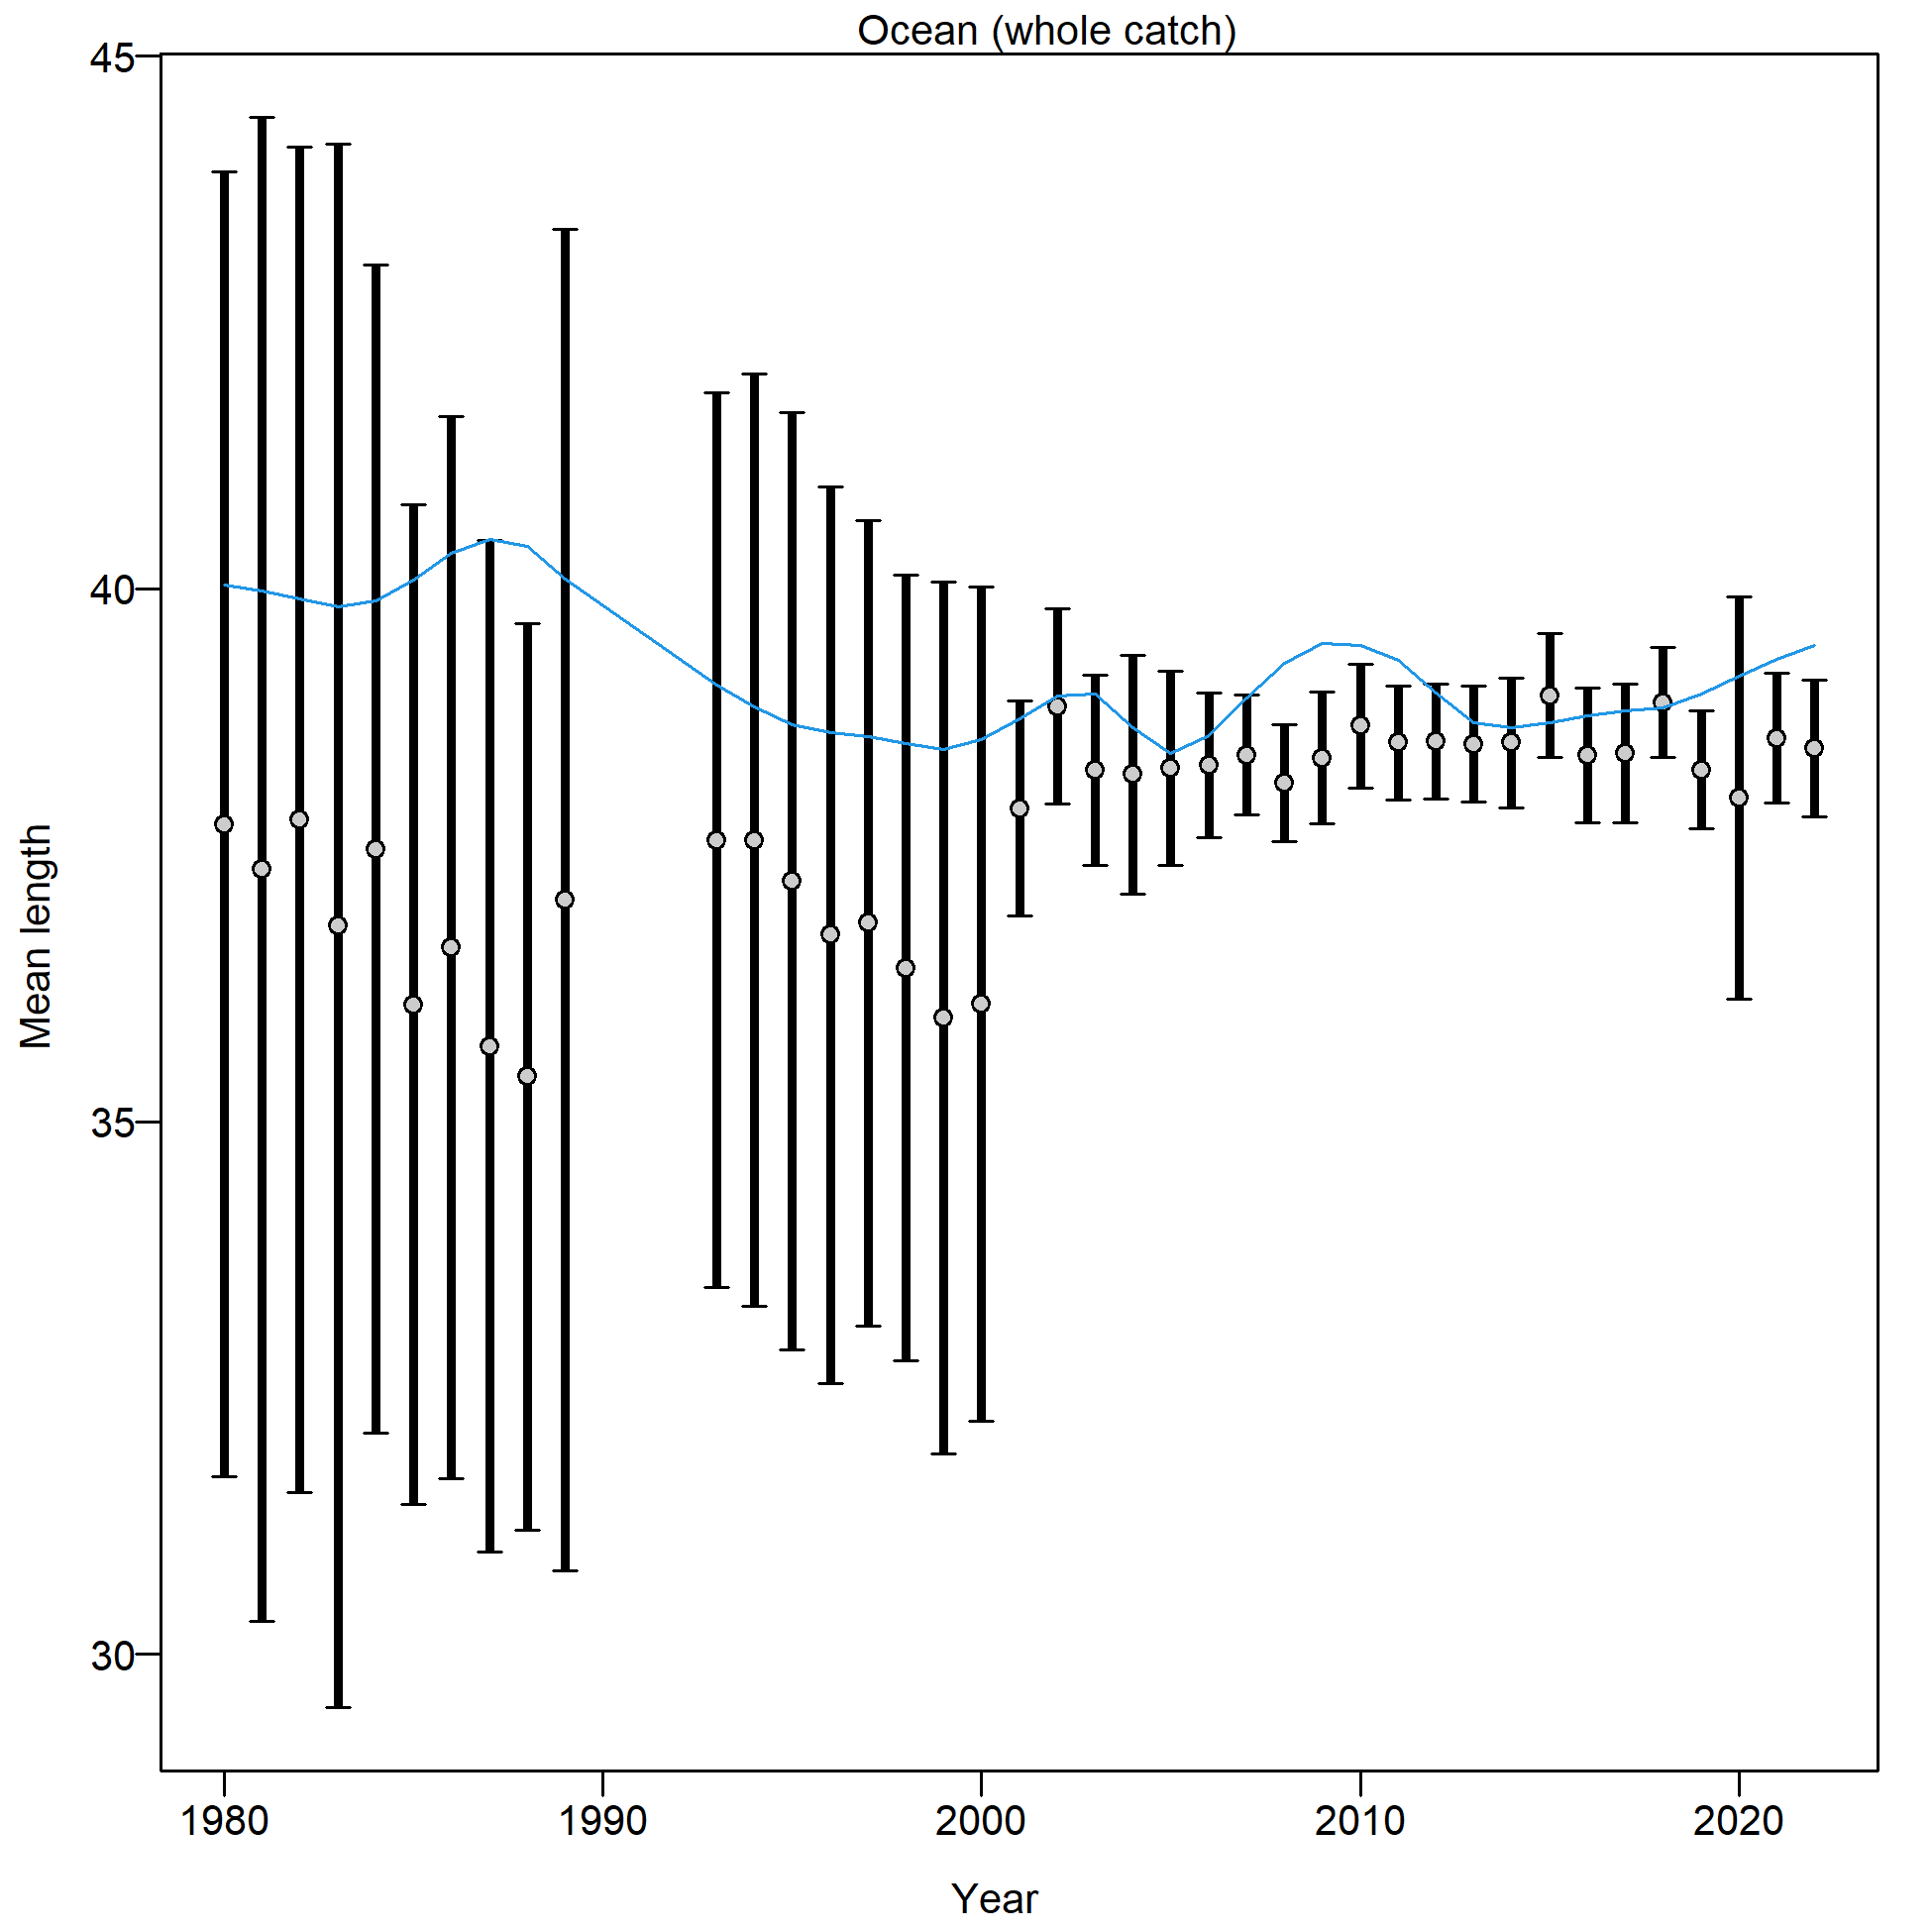
\includegraphics[width=1\textwidth,height=1\textheight]{C:/Users/Jason.Cope/Documents/Github/Sebastes_melanops_OR/Document/models/Reference model/plots/comp_lenfit_data_weighting_TA1.8_Ocean.png}
\caption{Mean length (cm) index from the recreational ocean boat fishery with 95 percent confidence intervals based on sample sizes and data weighting.\label{fig:ocean-mean-len-fit}}
\end{figure}

\newpage

\begin{figure}
\centering
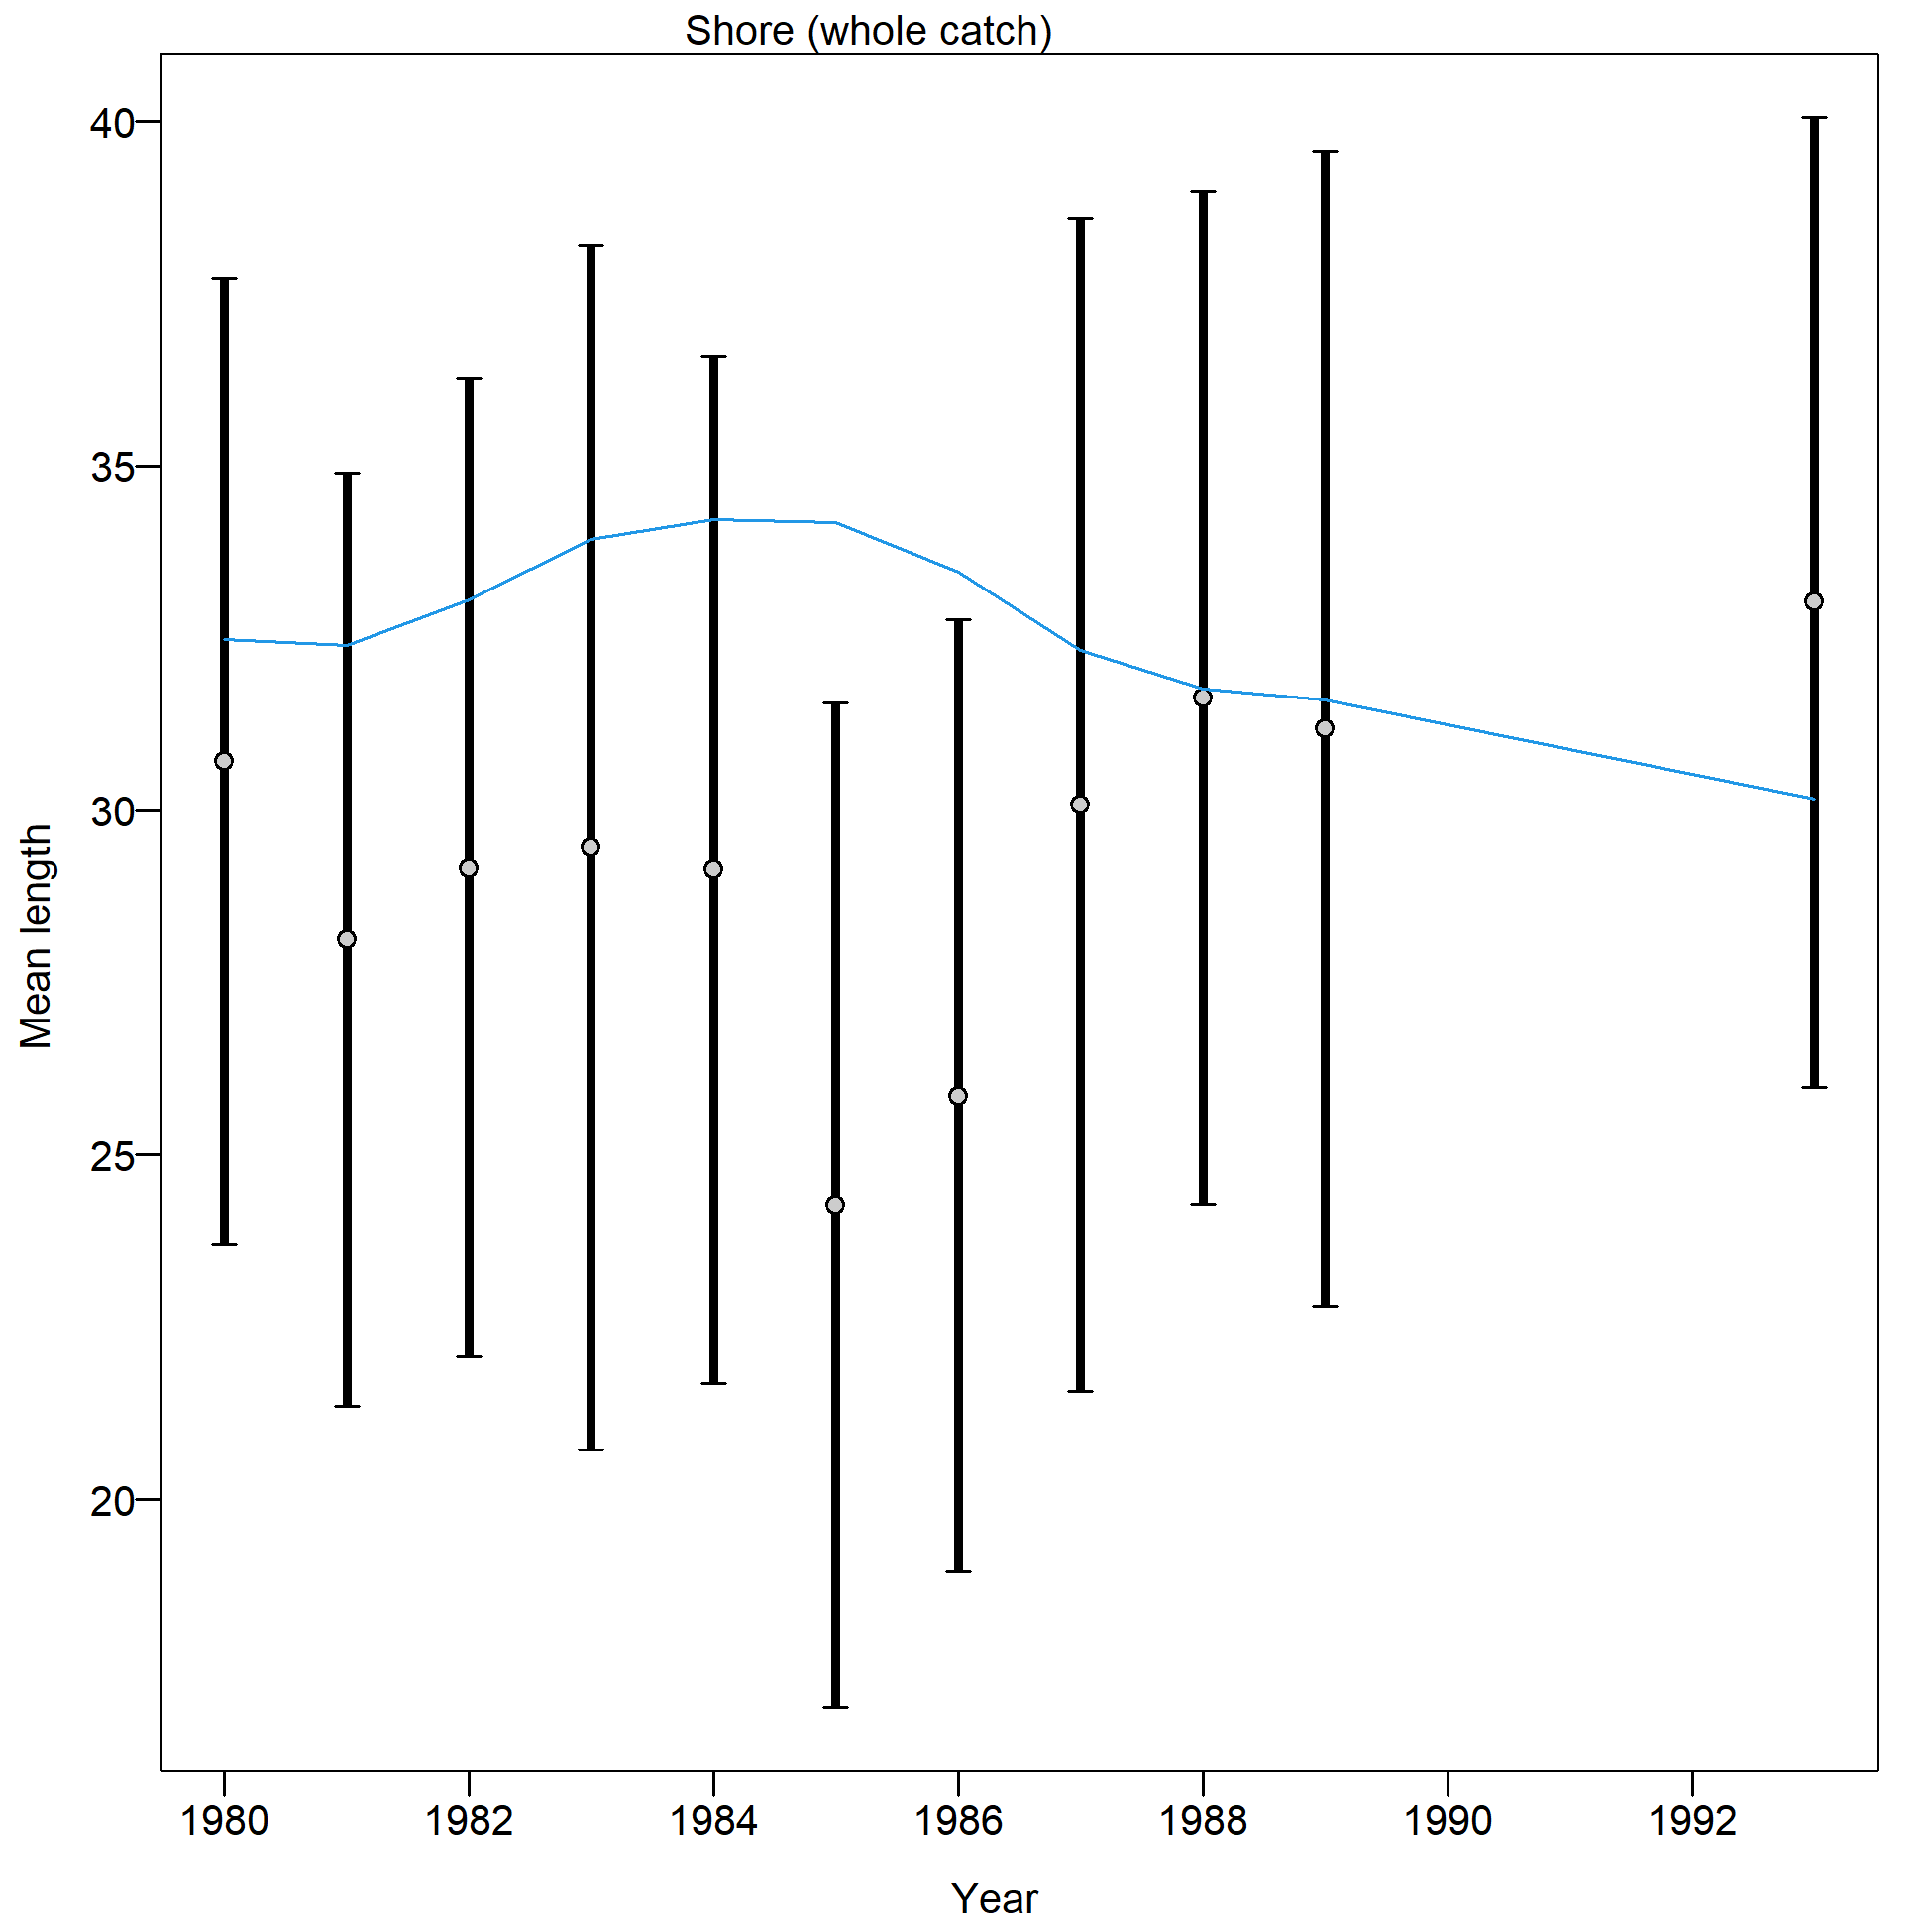
\includegraphics[width=1\textwidth,height=1\textheight]{C:/Users/Jason.Cope/Documents/Github/Sebastes_melanops_OR/Document/models/Reference model/plots/comp_lenfit_data_weighting_TA1.8_Shore.png}
\caption{Mean length (cm) index from the recreational shore-based fishery with 95 percent confidence intervals based on sample sizes and data weighting.\label{fig:shore-mean-len-fit}}
\end{figure}

\newpage

\begin{figure}
\centering
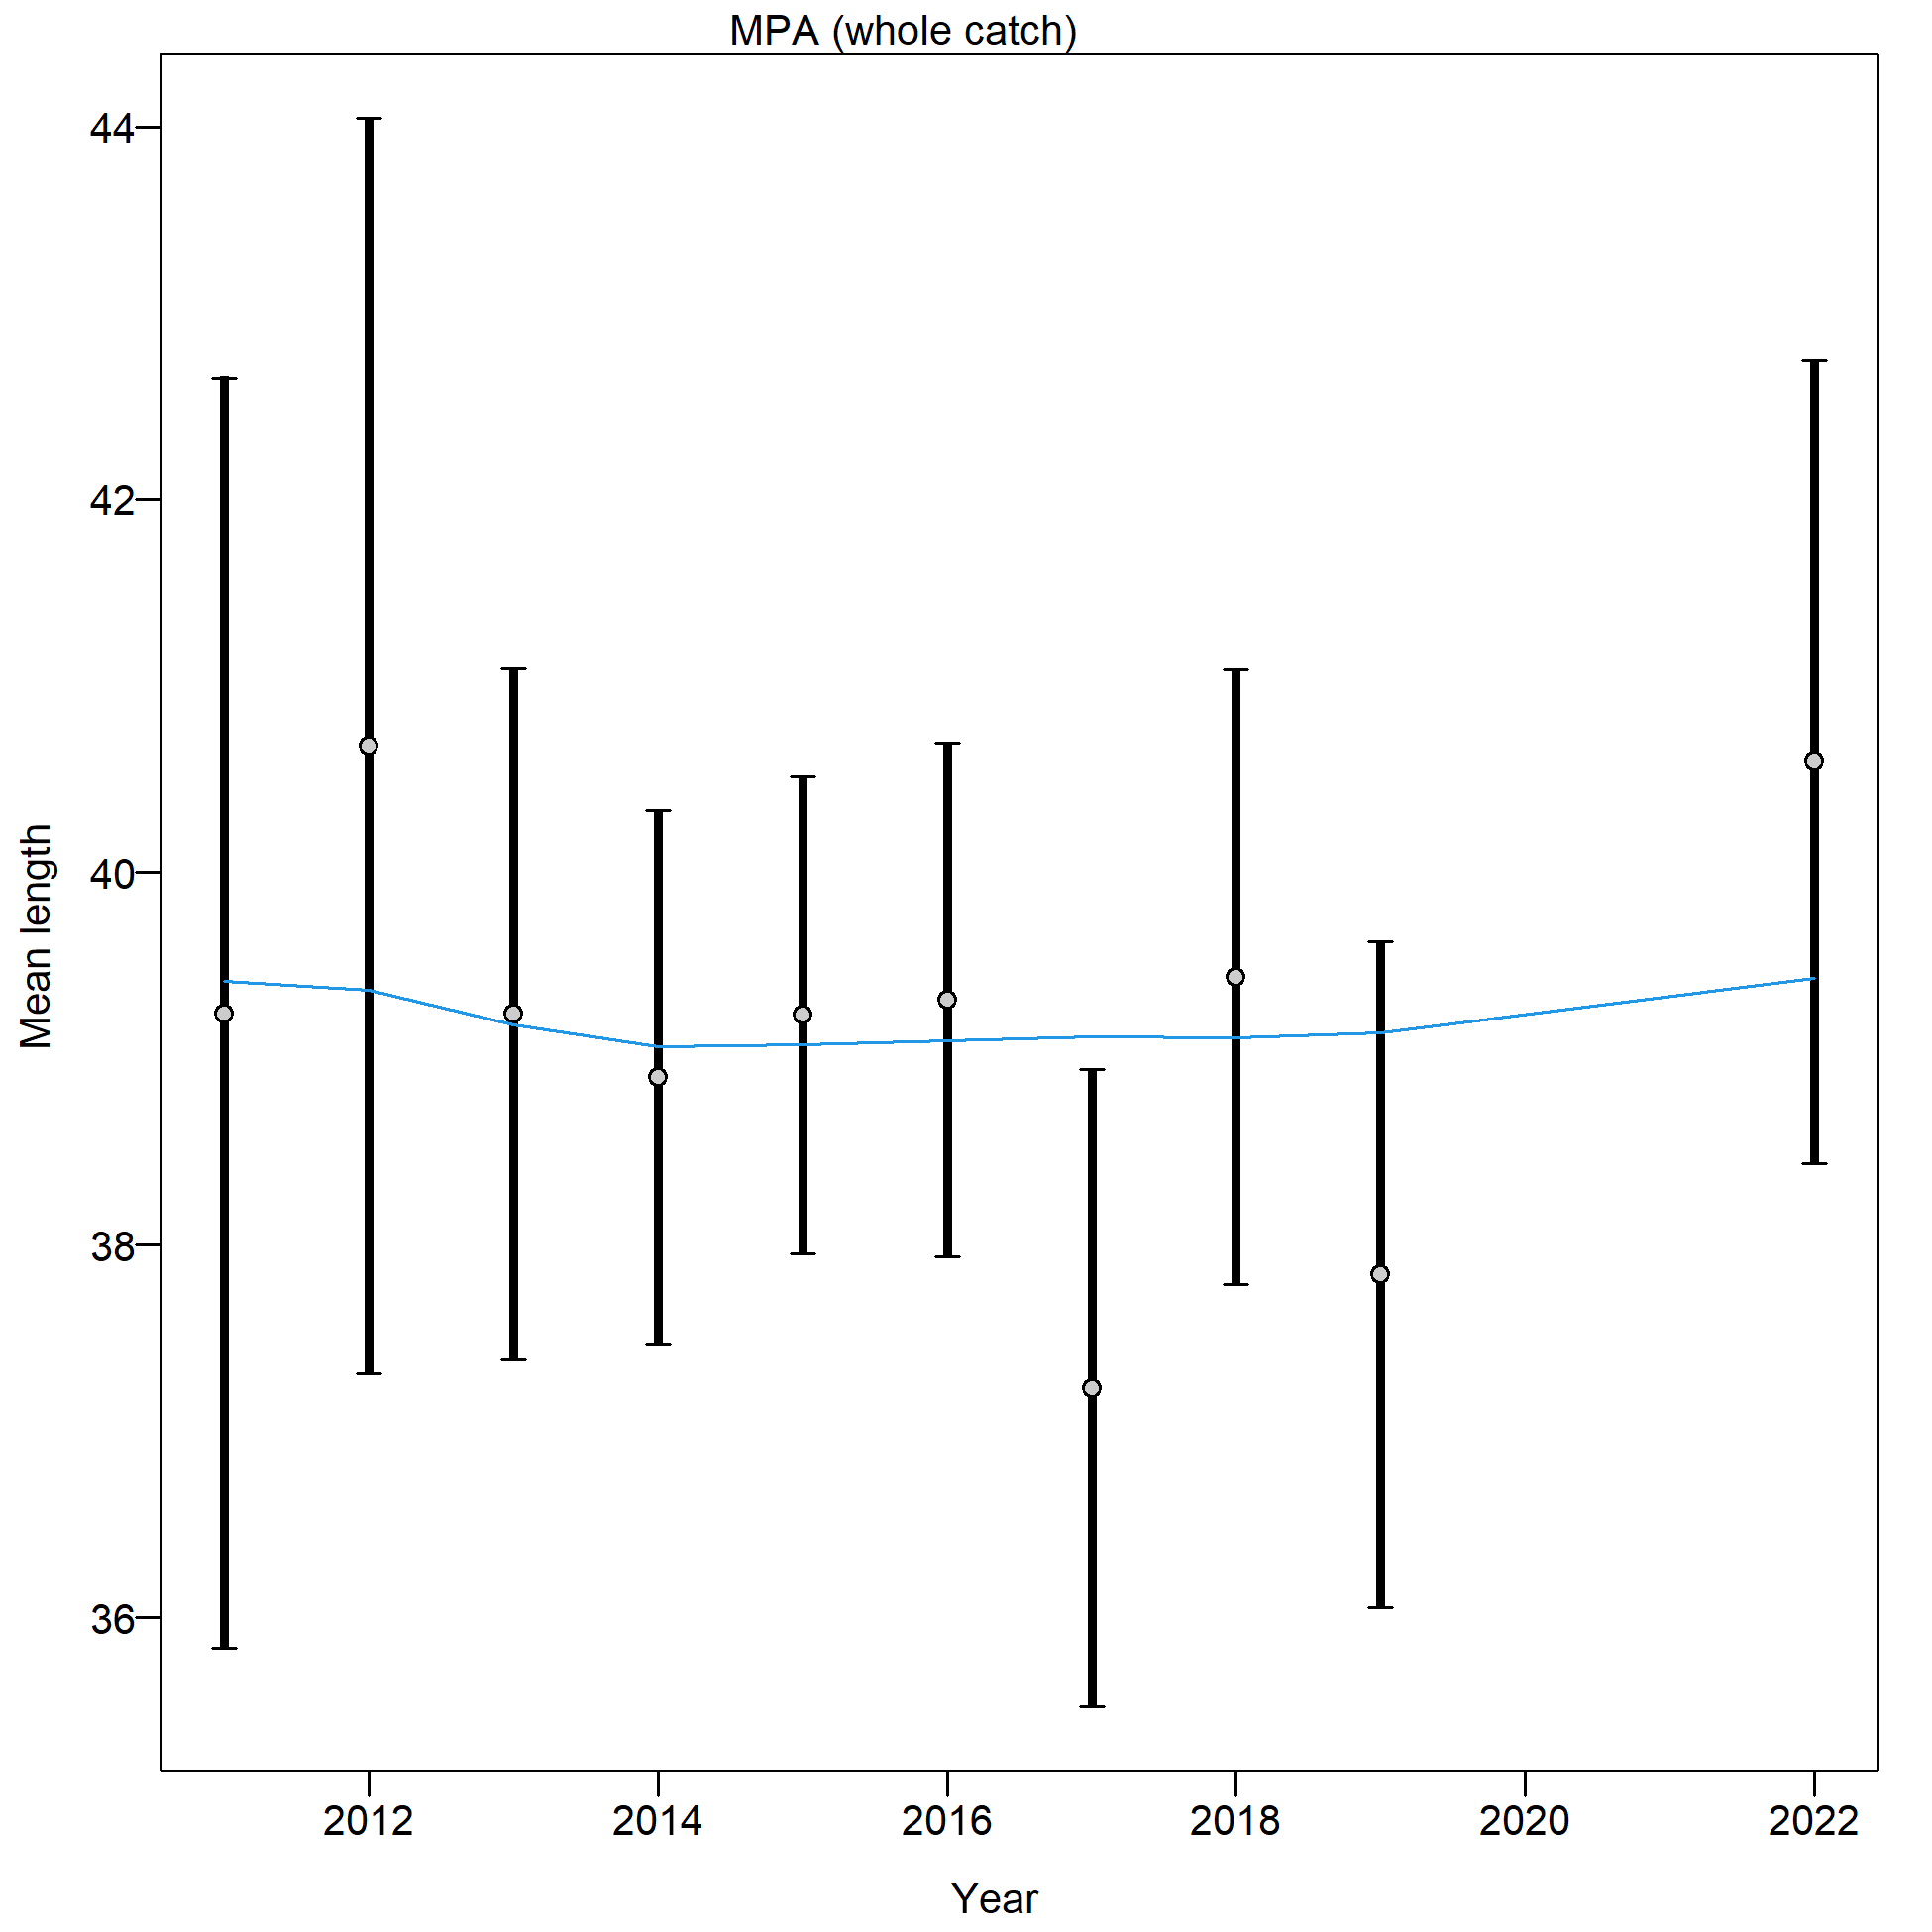
\includegraphics[width=1\textwidth,height=1\textheight]{C:/Users/Jason.Cope/Documents/Github/Sebastes_melanops_OR/Document/models/Reference model/plots/comp_lenfit_data_weighting_TA1.8_MPA.png}
\caption{Mean length (cm) index from the MPA survey with 95 percent confidence intervals based on sample sizes and data weighting.\label{fig:mpa-mean-len-fit}}
\end{figure}

\newpage

\begin{figure}
\centering
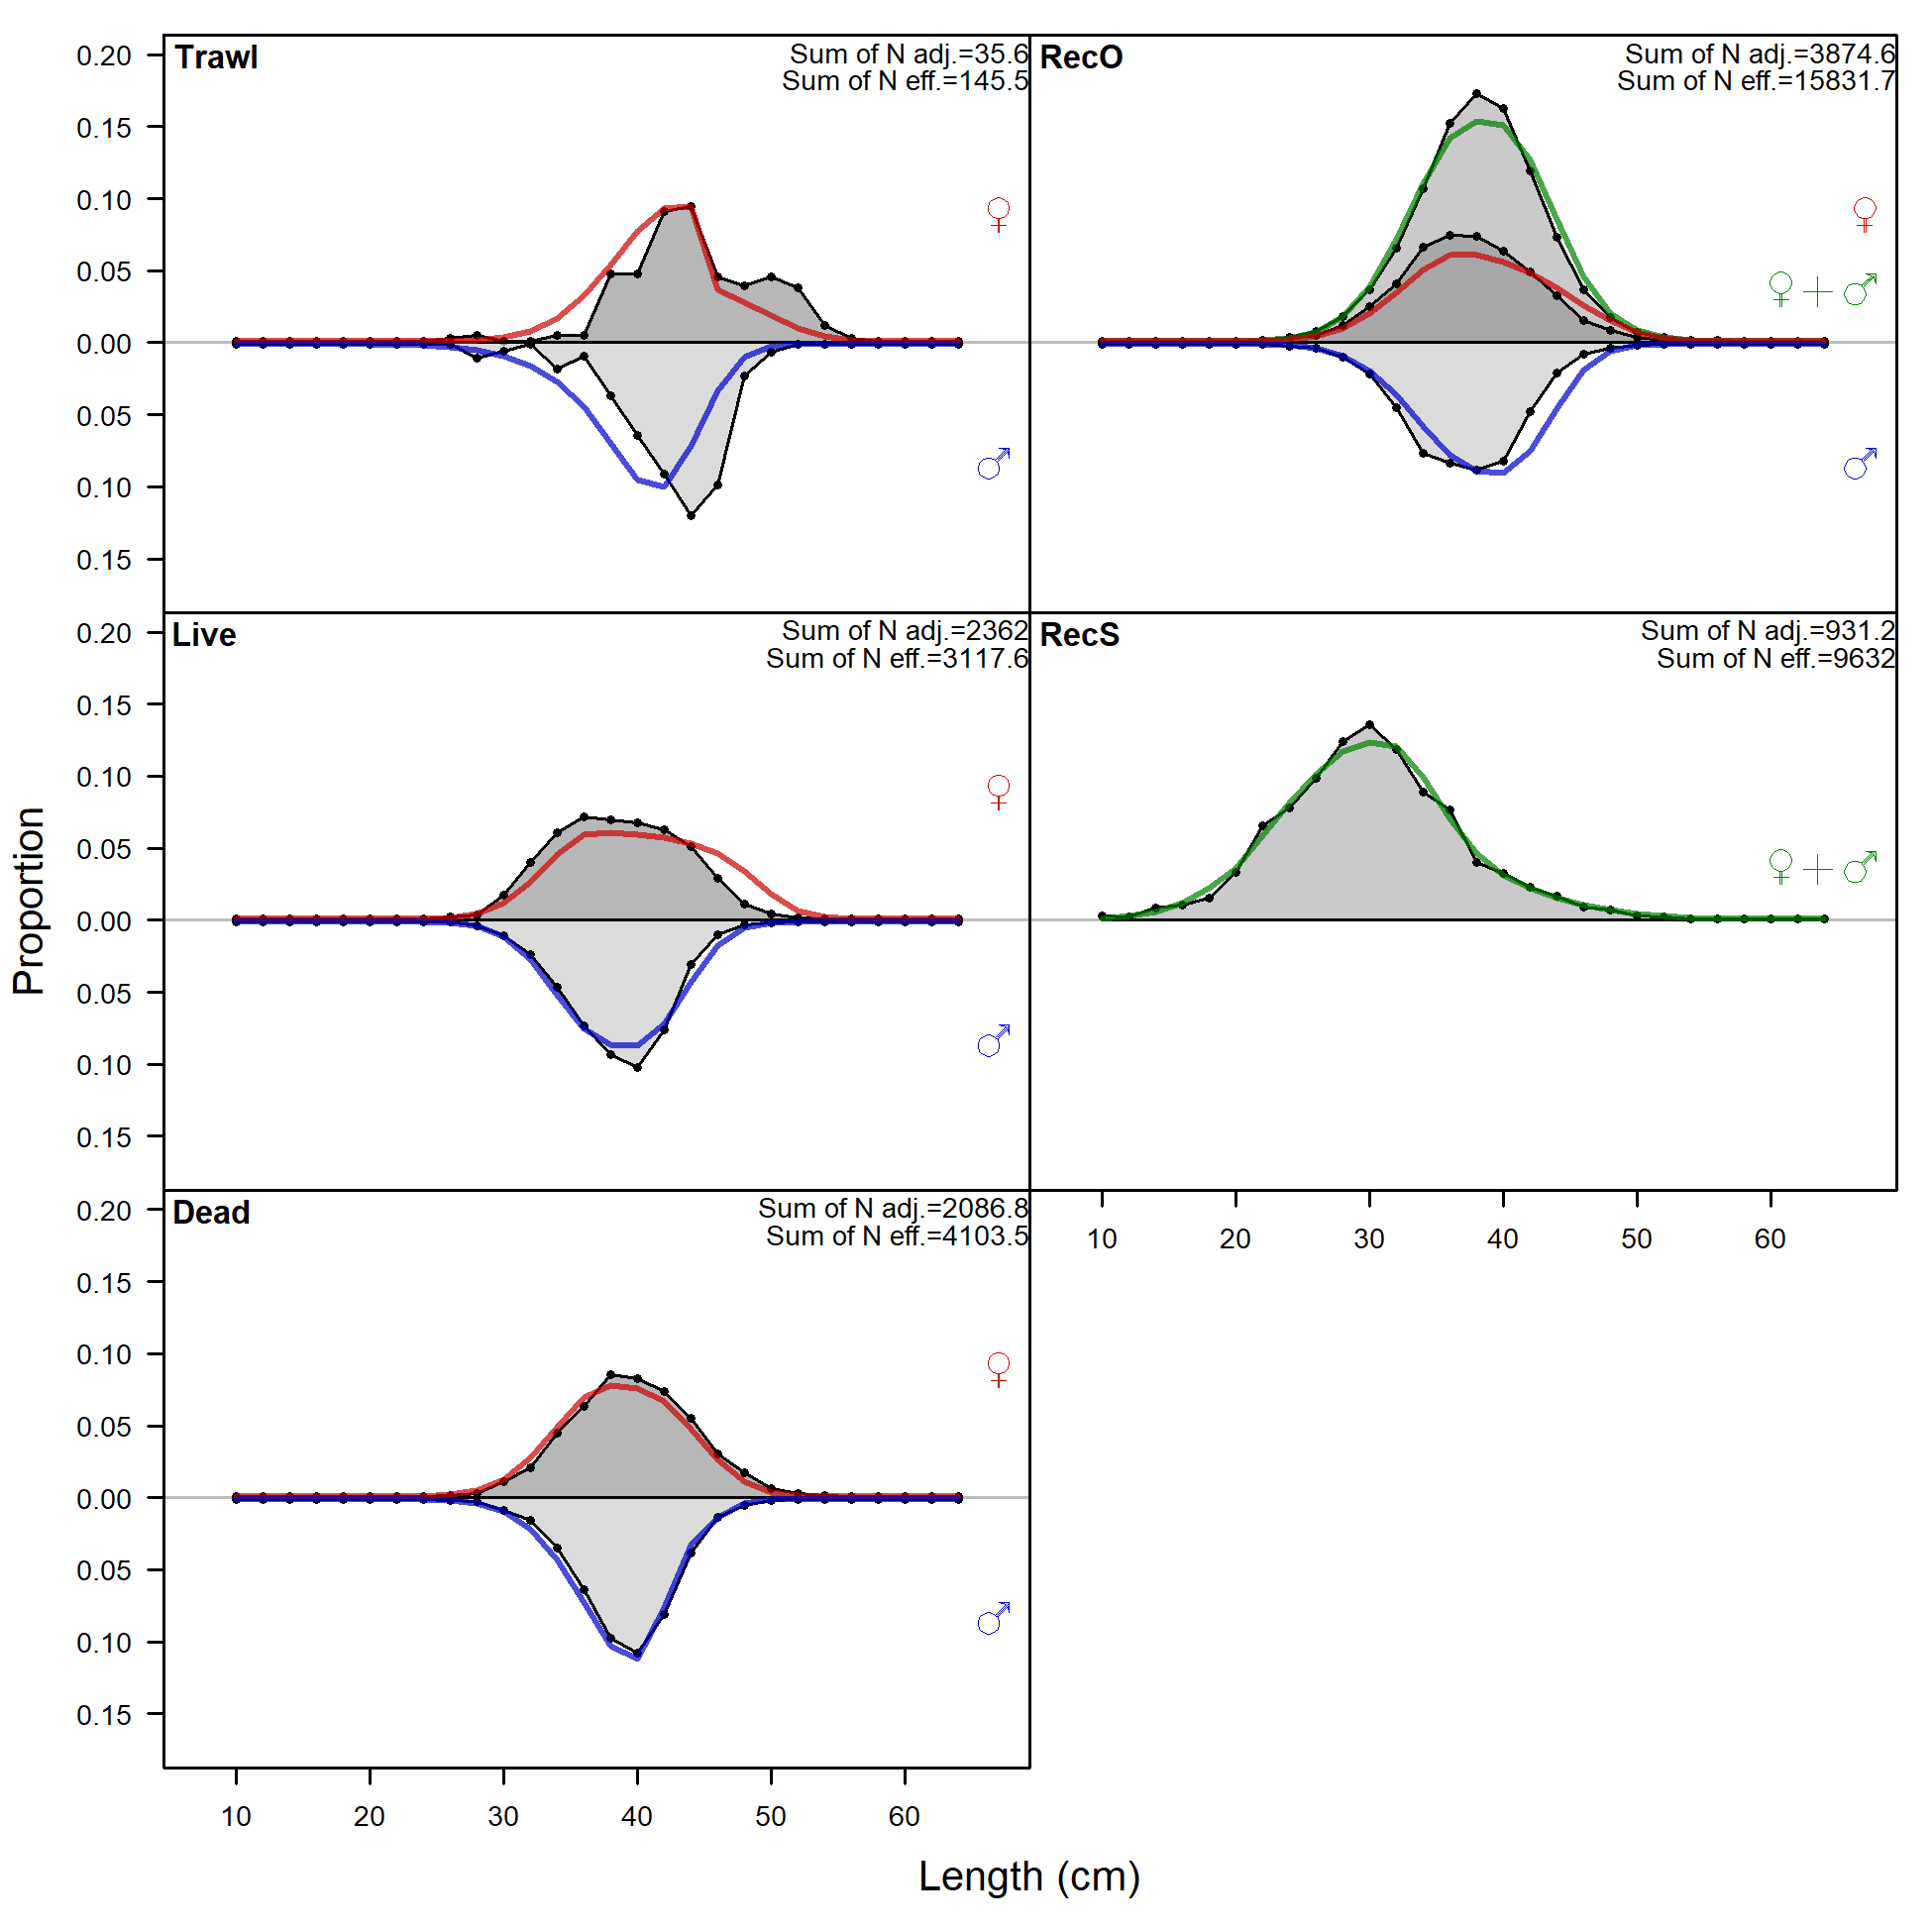
\includegraphics[width=1\textwidth,height=1\textheight]{C:/Users/Jason.Cope/Documents/Github/Sebastes_melanops_OR/Document/models/Reference model/plots/comp_lenfit__aggregated_across_time.png}
\caption{Aggregated length (cm) compositions over all years.\label{fig:agg-len-fit}}
\end{figure}

\newpage

\begin{figure}
\centering
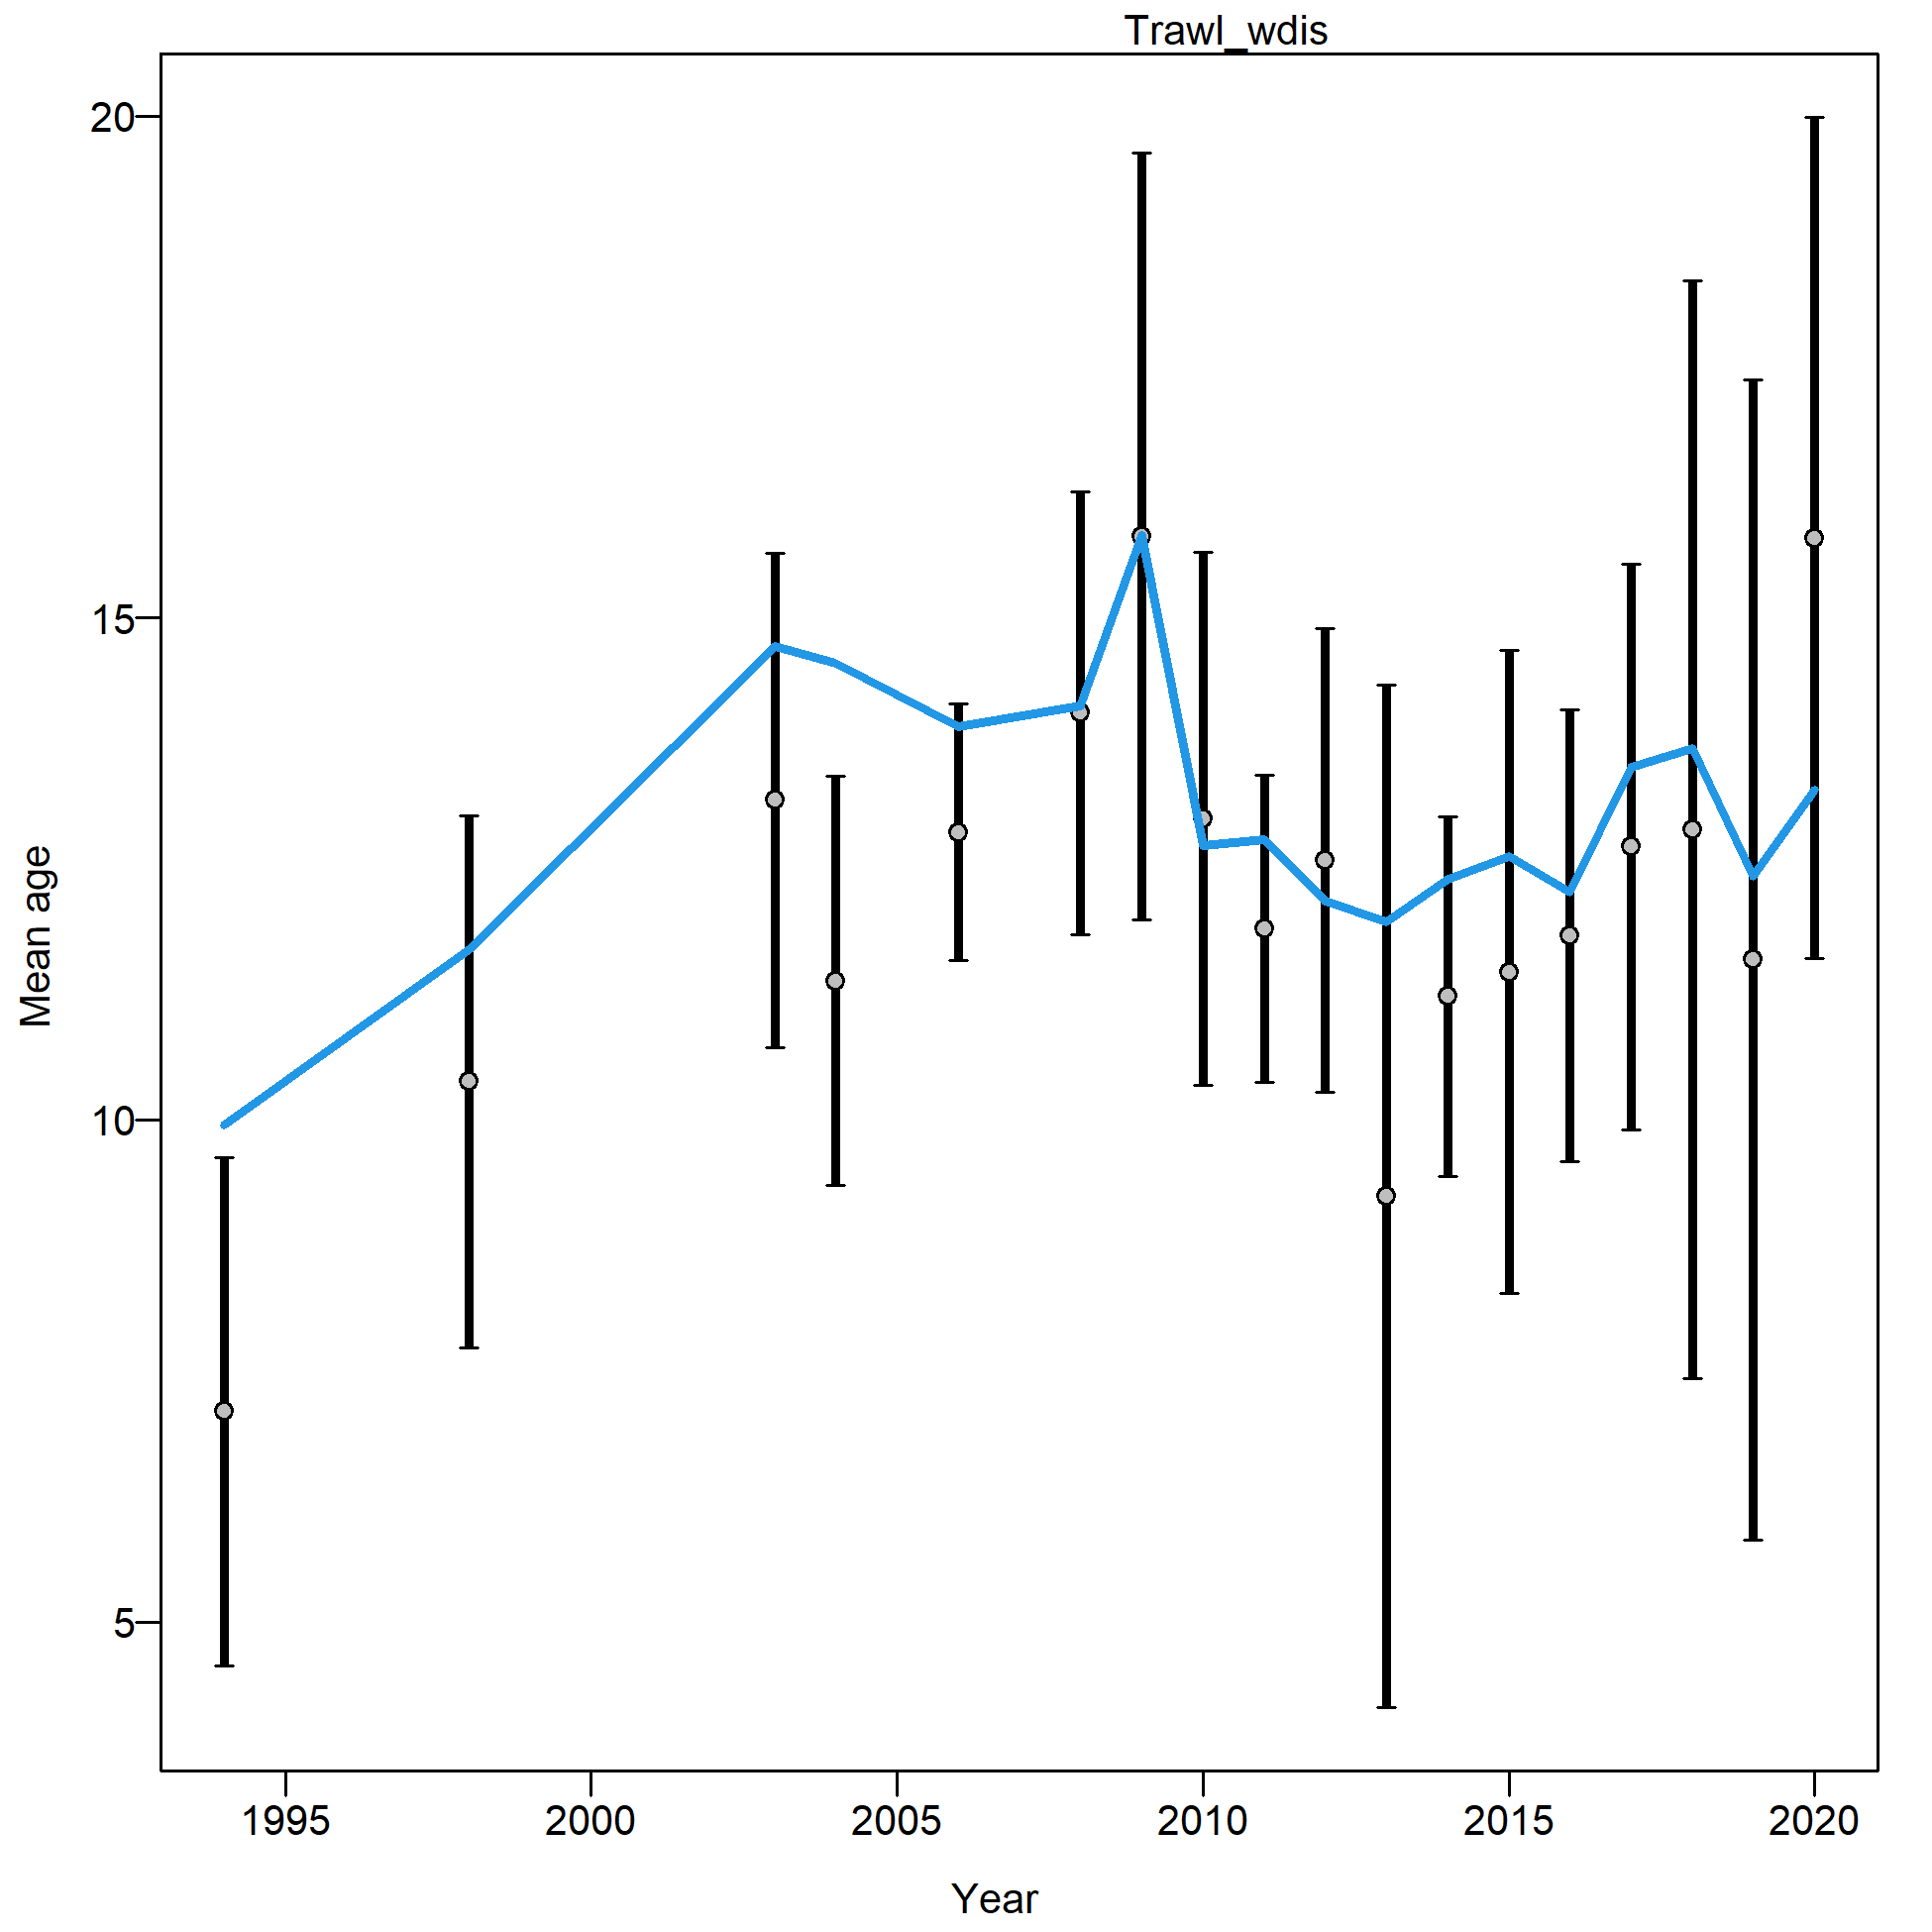
\includegraphics[width=1\textwidth,height=1\textheight]{C:/Users/Jason.Cope/Documents/Github/Sebastes_melanops_OR/Document/models/Reference model/plots/comp_condAALfit_data_weighting_TA1.8_condAgeTrawl_wdis.png}
\caption{Mean age from conditional age-at-length data for the commercial trawl fishery.\label{fig:trawl-mean-caal}}
\end{figure}

\newpage

\begin{figure}
\centering
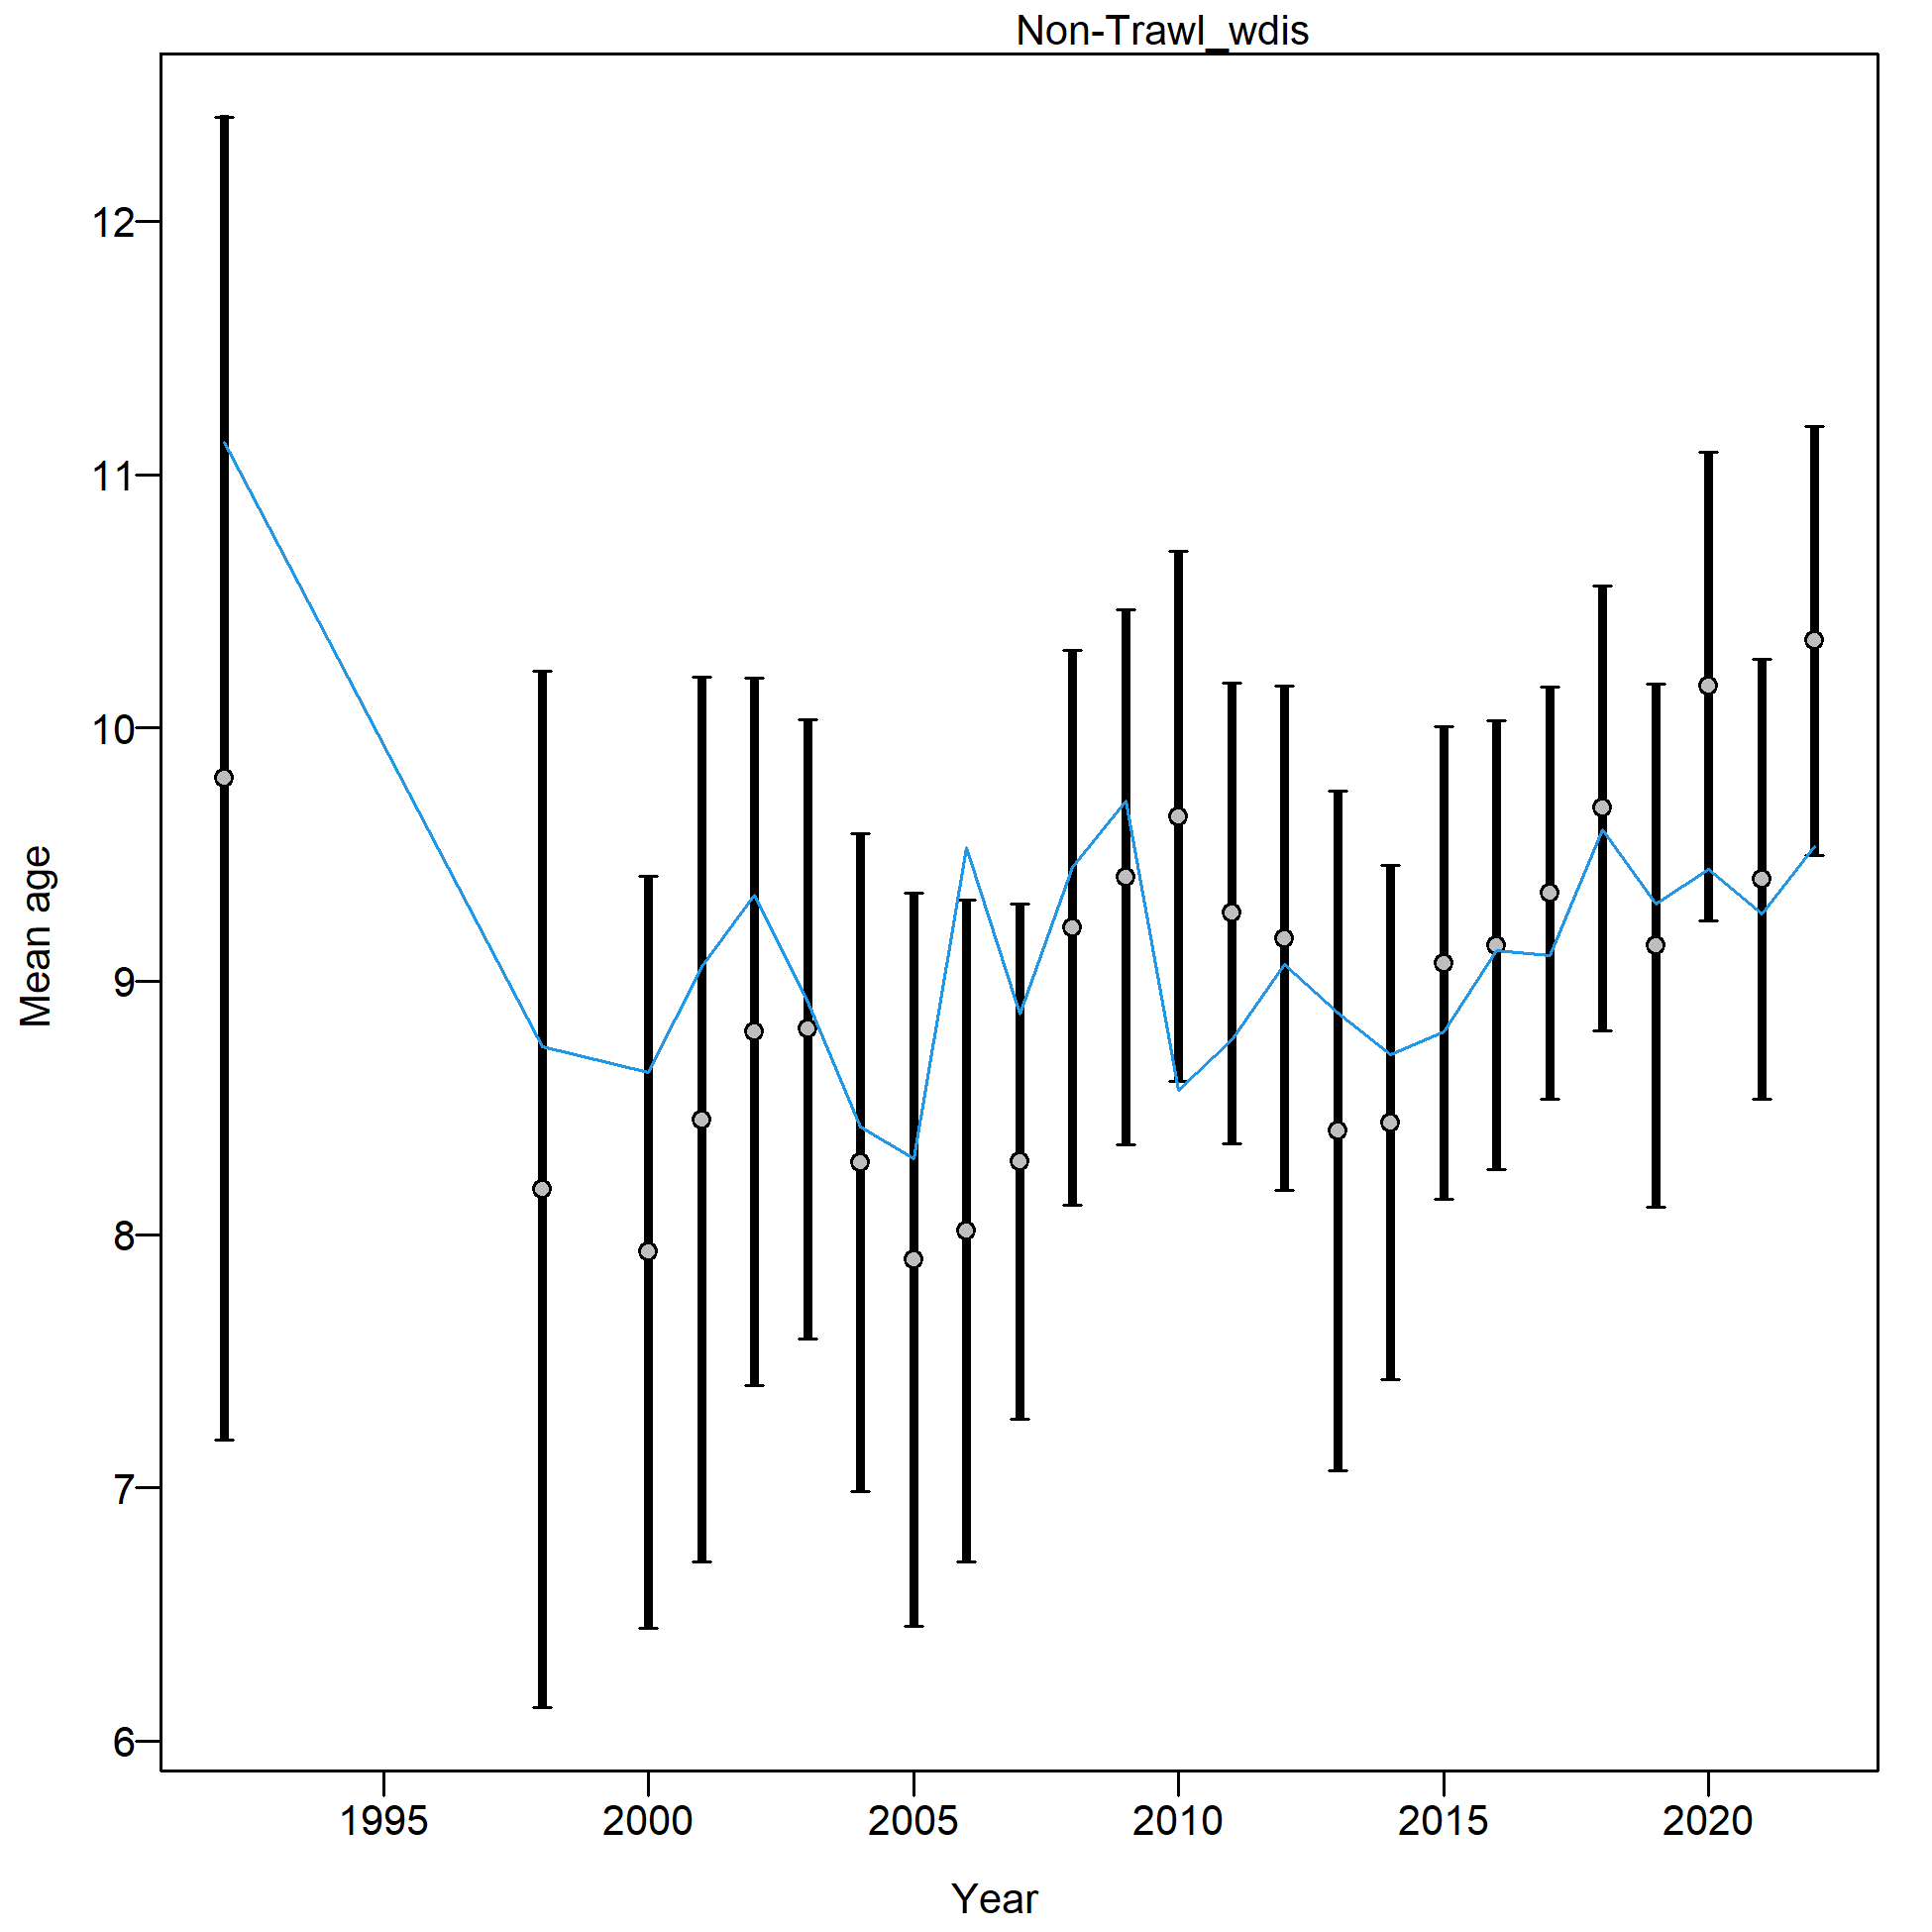
\includegraphics[width=1\textwidth,height=1\textheight]{C:/Users/Jason.Cope/Documents/Github/Sebastes_melanops_OR/Document/models/Reference model/plots/comp_condAALfit_data_weighting_TA1.8_condAgeNon-Trawl_wdis.png}
\caption{Mean age observations from the conditional age-at-length data from the non-trawl commercial fishery.\label{fig:nontrawl-mean-caal}}
\end{figure}

\newpage

\begin{figure}
\centering
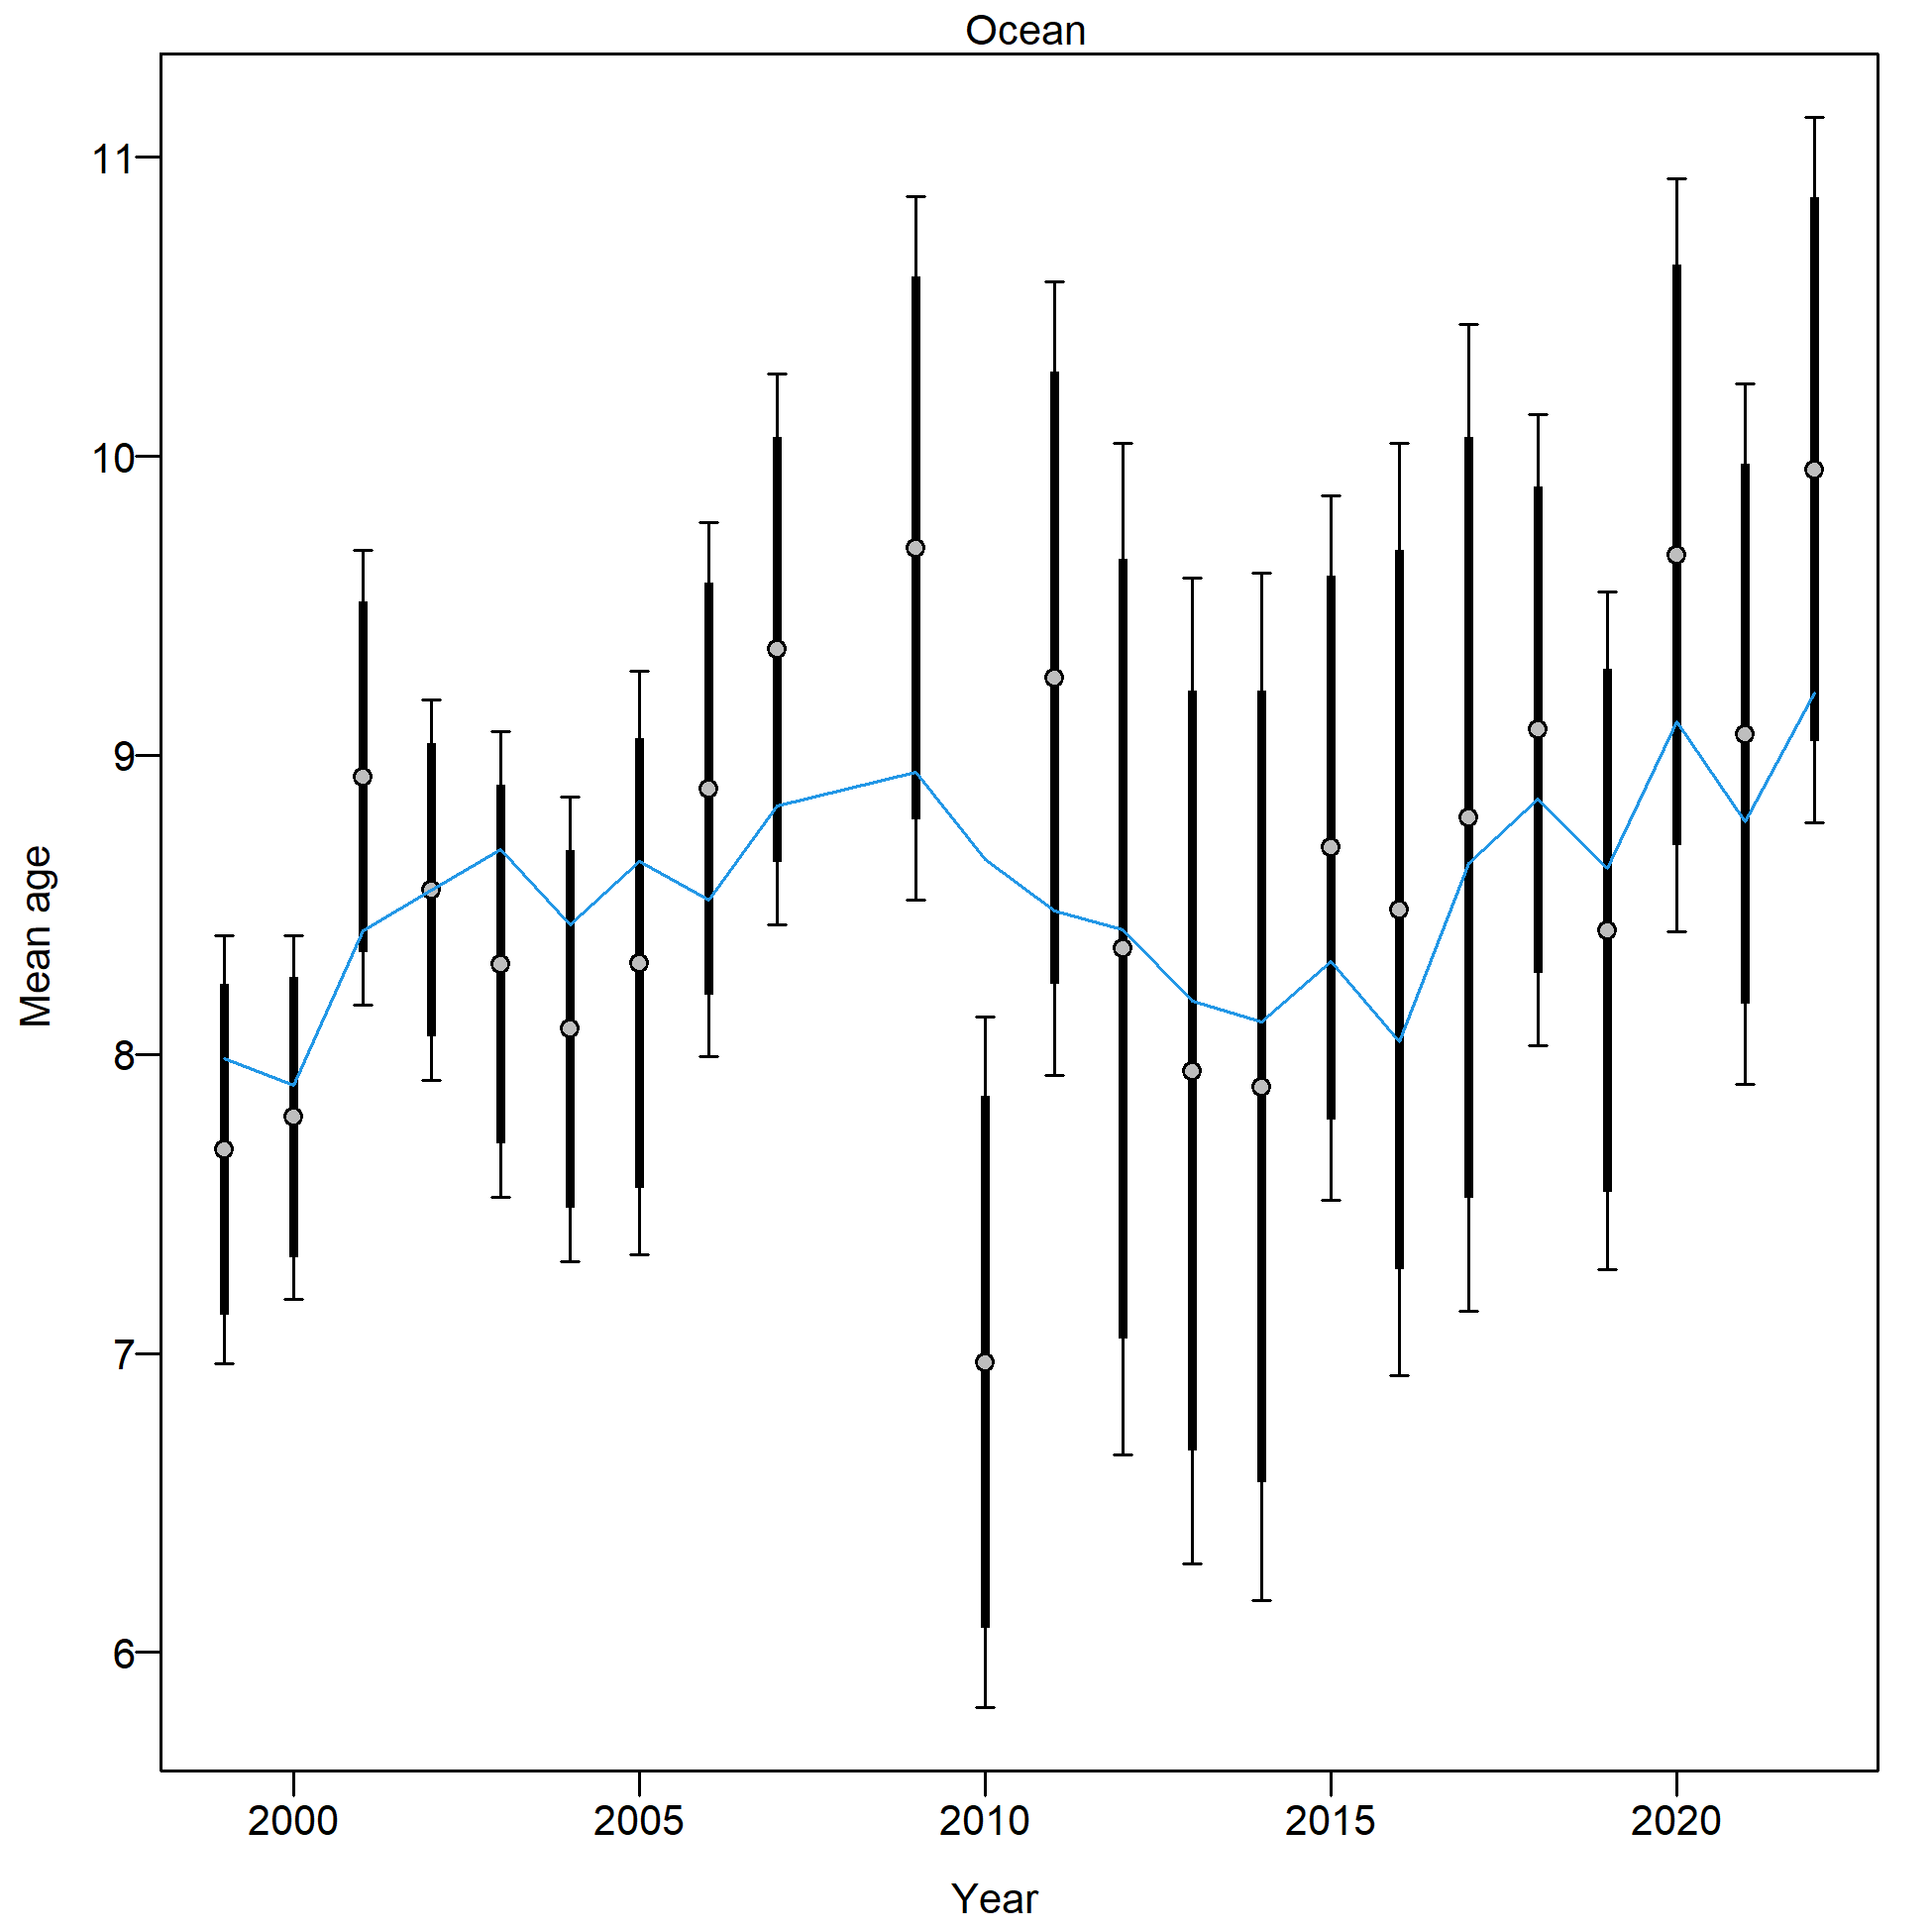
\includegraphics[width=1\textwidth,height=1\textheight]{C:/Users/Jason.Cope/Documents/Github/Sebastes_melanops_OR/Document/models/Reference model/plots/comp_condAALfit_data_weighting_TA1.8_condAgeOcean.png}
\caption{Mean age observations from the conditional age-at-length data from the ocean boat fishery.\label{fig:ocean-mean-caal}}
\end{figure}

\newpage

\begin{figure}
\centering
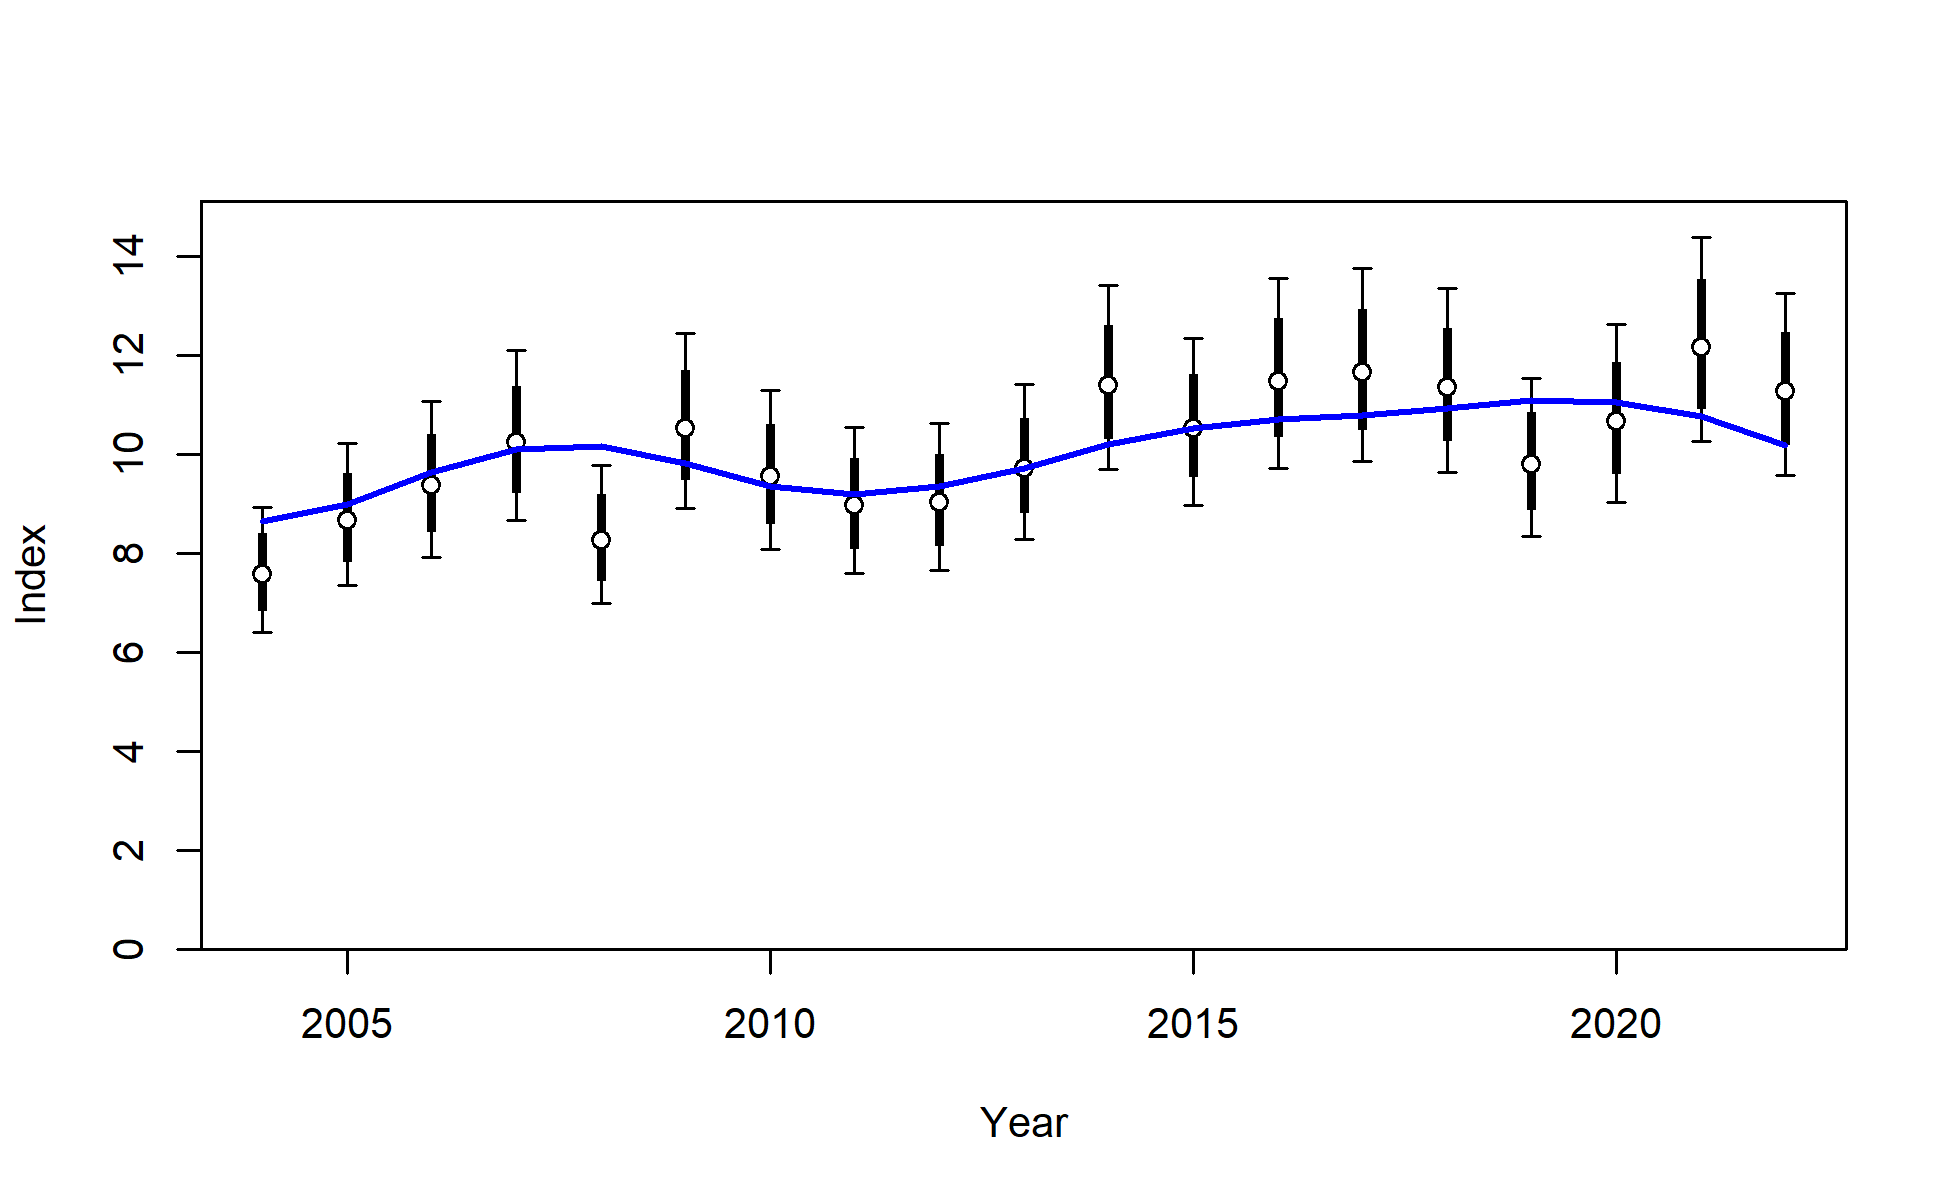
\includegraphics[width=1\textwidth,height=1\textheight]{C:/Users/Jason.Cope/Documents/Github/Sebastes_melanops_OR/Document/models/Reference model/plots/index2_cpuefit_Non-Trawl_wdis.png}
\caption{Fit to the non-trawl commercial survey index of abundance.\label{fig:nontrawl-index-fit}}
\end{figure}

\newpage

\begin{figure}
\centering
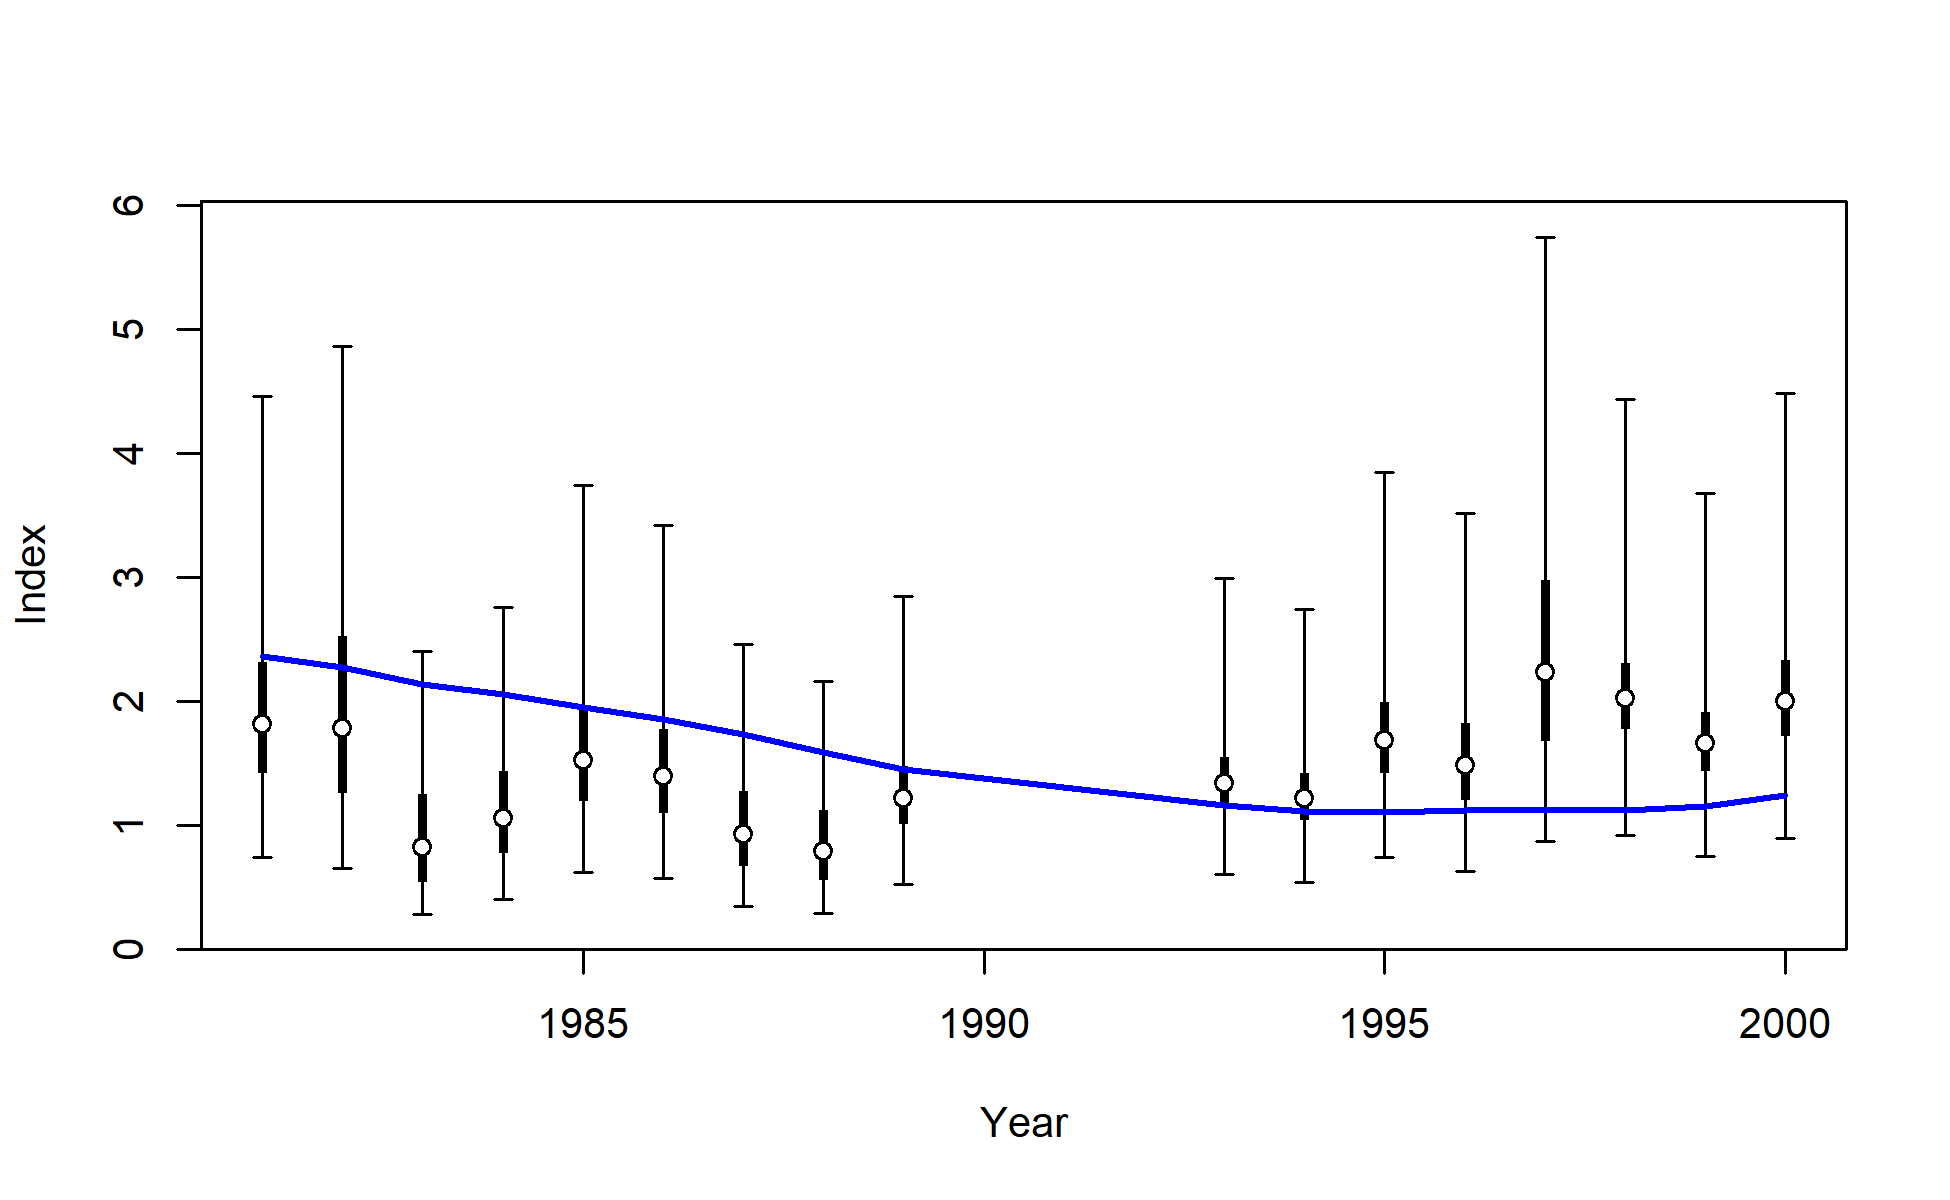
\includegraphics[width=1\textwidth,height=1\textheight]{C:/Users/Jason.Cope/Documents/Github/Sebastes_melanops_OR/Document/models/Reference model/plots/index2_cpuefit_MRFSS.png}
\caption{Fit to the MRFSS recreational survey index of abundance.\label{fig:mrfss-index-fit}}
\end{figure}

\newpage

\begin{figure}
\centering
\includegraphics[width=1\textwidth,height=1\textheight]{C:/Users/Jason.Cope/Documents/Github/Sebastes_melanops_OR/Document/models/Reference model/plots/index2_cpuefit_Ocean.png}
\caption{Fit to the ORBS recreational survey index of abundance.\label{fig:orbs-index-fit}}
\end{figure}

\newpage

\begin{figure}
\centering
\includegraphics[width=1\textwidth,height=1\textheight]{C:/Users/Jason.Cope/Documents/Github/Sebastes_melanops_OR/Document/models/Reference model/plots/index2_cpuefit_Tag.png}
\caption{Fit to the tagging survey index of abundance.\label{fig:tag-index-fit}}
\end{figure}

\newpage

\begin{figure}
\centering
\includegraphics[width=1\textwidth,height=1\textheight]{C:/Users/Jason.Cope/Documents/Github/Sebastes_melanops_OR/Document/models/Reference model/plots/index2_cpuefit_MPA.png}
\caption{Fit to the MPA survey index of abundance.\label{fig:mpa-index-fit}}
\end{figure}

\newpage

\hypertarget{estimated-recruitment}{%
\subsubsection{Estimated Recruitment}\label{estimated-recruitment}}

\begin{figure}
\centering
\includegraphics[width=1\textwidth,height=1\textheight]{C:/Users/Jason.Cope/Documents/Github/Sebastes_melanops_OR/Document/models/Reference model/plots/ts11_Age-0_recruits_(1000s)_with_95_asymptotic_intervals.png}
\caption{Estimated time series of age-0 recruits (1000s).\label{fig:recruits}}
\end{figure}

\newpage

\begin{figure}
\centering
\includegraphics[width=1\textwidth,height=1\textheight]{C:/Users/Jason.Cope/Documents/Github/Sebastes_melanops_OR/Document/models/Reference model/plots/recdevs2_withbars.png}
\caption{Estimated time series of recruitment deviations.\label{fig:rec-devs}}
\end{figure}

\newpage

\begin{figure}
\centering
\includegraphics[width=1\textwidth,height=1\textheight]{C:/Users/Jason.Cope/Documents/Github/Sebastes_melanops_OR/Document/models/Reference model/plots/recdevs3_varcheck.png}
\caption{Recruitment deviations variance by year. This plot tracks the information content contained in each recruitment deviation. Values below the red line (assumed recruitment variability) indicates years with more informed recruitment deviations.\label{fig:rec-devs-sigmas}}
\end{figure}

\newpage

\begin{figure}
\centering
\includegraphics[width=1\textwidth,height=1\textheight]{C:/Users/Jason.Cope/Documents/Github/Sebastes_melanops_OR/Document/models/Reference model/plots/SR_curve.png}
\caption{Stock-recruit curve. Point colors indicate year, with warmer colors indicating earlier years and cooler colors in showing later years.\label{fig:bh-curve}}
\end{figure}

\newpage

\begin{figure}
\centering
\includegraphics[width=1\textwidth,height=1\textheight]{C:/Users/Jason.Cope/Documents/Github/Sebastes_melanops_OR/Document/models/Reference model/plots/recruit_fit_bias_adjust.png}
\caption{Recruitment bias adjustment applied in the reference model.\label{fig:bias-adj}}
\end{figure}

\newpage

\begin{figure}
\centering
\includegraphics[width=1\textwidth,height=1\textheight]{C:/Users/Jason.Cope/Documents/Github/Sebastes_melanops_OR/Document/models/Reference model/plots/recdevs3_varcheck.png}
\caption{Recruitment deviations variance check. Low standard deviations indicate years with informative deviations .\label{fig:varcheck}}
\end{figure}

\newpage

\hypertarget{selectivity}{%
\subsubsection{Selectivity}\label{selectivity}}

\begin{figure}
\centering
\includegraphics[width=1\textwidth,height=1\textheight]{C:/Users/Jason.Cope/Documents/Github/Sebastes_melanops_OR/Document/models/Reference model/plots/sel01_multiple_fleets_length1.png}
\caption{Length-based selectivity curves for each fleet and survey.\label{fig:fleet-selectivity}}
\end{figure}

\newpage

\hypertarget{time-series}{%
\subsubsection{Time Series}\label{time-series}}

\begin{figure}
\centering
\includegraphics[width=1\textwidth,height=1\textheight]{C:/Users/Jason.Cope/Documents/Github/Sebastes_melanops_OR/Document/models/Reference model/plots/ts7_Spawning_output_with_95_asymptotic_intervals_intervals.png}
\caption{Estimated time series of spawning output (in millions of eggs).\label{fig:ssb}}
\end{figure}

\newpage

\begin{figure}
\centering
\includegraphics[width=1\textwidth,height=1\textheight]{C:/Users/Jason.Cope/Documents/Github/Sebastes_melanops_OR/Document/models/Reference model/plots/ts1_Total_biomass_(mt).png}
\caption{Estimated time series of total biomass (mt).\label{fig:tot-bio}}
\end{figure}

\newpage

\begin{figure}
\centering
\includegraphics[width=1\textwidth,height=1\textheight]{C:/Users/Jason.Cope/Documents/Github/Sebastes_melanops_OR/Document/models/Reference model/plots/ts9_Relative_spawning_output_intervals.png}
\caption{Estimated time series of fraction of unfished spawning output.\label{fig:depl}}
\end{figure}

\newpage

\hypertarget{comparison-to-previous-assessments}{%
\subsubsection{Comparison to Previous Assessments}\label{comparison-to-previous-assessments}}

\begin{figure}
\centering
\includegraphics[width=1\textwidth,height=1\textheight]{C:/Users/Jason.Cope/Documents/Github/Sebastes_melanops_OR/Document/figures/comp_2015_2023/compare2_spawnbio_uncertainty.png}
\caption{Comparison of the time series of spawning output between the 2015 and 2023 assessment results.\label{fig:comp-ssb}}
\end{figure}

\newpage

\begin{figure}
\centering
\includegraphics[width=1\textwidth,height=1\textheight]{C:/Users/Jason.Cope/Documents/Github/Sebastes_melanops_OR/Document/figures/comp_2015_2023/compare4_Bratio_uncertainty.png}
\caption{Comparison of the time series of relative spawning output between the 2015 and 2023 assessment results.\label{fig:comp-depl}}
\end{figure}

\newpage

\hypertarget{sensitivities}{%
\subsubsection{Sensitivities}\label{sensitivities}}

\begin{figure}
\centering
\includegraphics[width=1\textwidth,height=1\textheight]{C:/Users/Jason.Cope/Documents/Github/Sebastes_melanops_OR/Document/figures/sensi_data/Sensi_logREplot_SB_Dep_F_MSY.png}
\caption{Log relative change (log((Model\_sensi-Model\_ref)/Model\_ref)) in data treatment for 5 derived quantities. Colored boxes indicate 95 percent confidence interval of the reference model.\label{fig:sensi-data-RE}}
\end{figure}

\newpage

\begin{figure}
\centering
\includegraphics[width=1\textwidth,height=1\textheight]{C:/Users/Jason.Cope/Documents/Github/Sebastes_melanops_OR/Document/figures/sensi_data/compare2_spawnbio_uncertainty.png}
\caption{Spawning output (in millions of eggs) time series by data treatment compared to the reference model.\label{fig:sensi-data-ssb}}
\end{figure}

\newpage

\begin{figure}
\centering
\includegraphics[width=1\textwidth,height=1\textheight]{C:/Users/Jason.Cope/Documents/Github/Sebastes_melanops_OR/Document/figures/sensi_data/compare4_Bratio_uncertainty.png}
\caption{Relative spawning output time series by data treatment compared to the reference model. Missing scenarios mean the spawning output was too large to show.\label{fig:sensi-data-depl}}
\end{figure}

\newpage

\begin{figure}
\centering
\includegraphics[width=1\textwidth,height=1\textheight]{C:/Users/Jason.Cope/Documents/Github/Sebastes_melanops_OR/Document/figures/sensi_modspex/Sensi_logREplot_SB_Dep_F_MSY.png}
\caption{Log relative change (log((Model\_sensi-Model\_ref)/Model\_ref)) in model specification scenario for 5 derived quantities. Colored boxes indicate 95 percent confidence interval of the reference model.\label{fig:sensi-modspec-RE}}
\end{figure}

\newpage

\begin{figure}
\centering
\includegraphics[width=1\textwidth,height=1\textheight]{C:/Users/Jason.Cope/Documents/Github/Sebastes_melanops_OR/Document/figures/sensi_modspex/compare2_spawnbio_uncertainty.png}
\caption{Spawning output (in millions of eggs) time series by model specification scenario compared to the reference model. Missing scenarios mean the spawning output was too large to show.\label{fig:sensi-modspec-ssb}}
\end{figure}

\newpage

\begin{figure}
\centering
\includegraphics[width=1\textwidth,height=1\textheight]{C:/Users/Jason.Cope/Documents/Github/Sebastes_melanops_OR/Document/figures/sensi_modspex/compare4_Bratio_uncertainty.png}
\caption{Relative spawning output time series by model specification scenario compared to the reference model.\label{fig:sensi-modspec-depl}}
\end{figure}

\newpage

\hypertarget{likelihood-profiles-1}{%
\subsubsection{Likelihood Profiles}\label{likelihood-profiles-1}}

\begin{figure}
\centering
\includegraphics[width=1\textwidth,height=1\textheight]{C:/Users/Jason.Cope/Documents/Github/Sebastes_melanops_OR/Document/figures/likelihoods/parameter_panel_LnQ_base_Acoustic_Visual(6).png}
\caption{Acoustic-visual survey catchability likelihood profile (change in the negative log-likelihood across a range of catchability values) and derived quantities.\label{fig:AVq-profile}}
\end{figure}

\newpage

\begin{figure}
\centering
\includegraphics[width=1\textwidth,height=1\textheight]{C:/Users/Jason.Cope/Documents/Github/Sebastes_melanops_OR/Document/figures/likelihoods/piner_panel_LnQ_base_Acoustic_Visual(6).png}
\caption{Acoustic-visual survey catchability likelihood profile for each of the likelihood components.\label{fig:AVq-profile-components}}
\end{figure}

\newpage

\begin{figure}
\centering
\includegraphics[width=1\textwidth,height=1\textheight]{C:/Users/Jason.Cope/Documents/Github/Sebastes_melanops_OR/Document/figures/likelihoods/parameter_panel_SR_BH_steep.png}
\caption{Beverton-Holt steepness parameter likelihood profile (change in the negative log-likelihood across a range of steepness values) and derived quantities.\label{fig:steepness-profile}}
\end{figure}

\newpage

\begin{figure}
\centering
\includegraphics[width=1\textwidth,height=1\textheight]{C:/Users/Jason.Cope/Documents/Github/Sebastes_melanops_OR/Document/figures/likelihoods/piner_panel_SR_BH_steep.png}
\caption{Beverton-Holt steepness parameter likelihood profile for each of the likelihood components.\label{fig:steepness-profile-components}}
\end{figure}

\newpage

\begin{figure}
\centering
\includegraphics[width=1\textwidth,height=1\textheight]{C:/Users/Jason.Cope/Documents/Github/Sebastes_melanops_OR/Document/figures/likelihoods/M_fm_multilikelihood_profile.png}
\caption{Female and male \(M\) multi-parameter likelihood profile and derived quantities. Red lines in the top left figure indicate significantly similar values compared to the reference model. Broken and solid lines in the bottom right figure indicate target and limit referene points, respectively.\label{fig:M-multiprofile-combo}}
\end{figure}

\newpage

\begin{figure}
\centering
\includegraphics[width=1\textwidth,height=1\textheight]{C:/Users/Jason.Cope/Documents/Github/Sebastes_melanops_OR/Document/figures/likelihoods/Piner_like_comps.png}
\caption{Likelihood component values for the female and male \(M\) multi-parameter likelihood profile.\label{fig:M-multiprofile-like-components}}
\end{figure}

\newpage

\begin{figure}
\centering
\includegraphics[width=1\textwidth,height=1\textheight]{C:/Users/Jason.Cope/Documents/Github/Sebastes_melanops_OR/Document/figures/likelihoods/LC_Lt.png}
\caption{Length likelihood component values for the female and male \(M\) multi-parameter likelihood profile.\label{fig:M-multiprofile-length-components}}
\end{figure}

\newpage

\begin{figure}
\centering
\includegraphics[width=1\textwidth,height=1\textheight]{C:/Users/Jason.Cope/Documents/Github/Sebastes_melanops_OR/Document/figures/likelihoods/LC_age.png}
\caption{Age likelihood component values for the female and male \(M\) multi-parameter likelihood profile.\label{fig:M-multiprofile-age-components}}
\end{figure}

\newpage

\begin{figure}
\centering
\includegraphics[width=1\textwidth,height=1\textheight]{C:/Users/Jason.Cope/Documents/Github/Sebastes_melanops_OR/Document/figures/likelihoods/LC_survey.png}
\caption{Survey likelihood component values for the female and male \(M\) multi-parameter likelihood profile.\label{fig:M-multiprofile-survey-components}}
\end{figure}

\newpage

\hypertarget{retrospectives}{%
\subsubsection{Retrospectives}\label{retrospectives}}

\begin{figure}
\centering
\includegraphics[width=1\textwidth,height=1\textheight]{C:/Users/Jason.Cope/Documents/Github/Sebastes_melanops_OR/Document/figures/retro/compare2_spawnbio_uncertainty.png}
\caption{Change in the estimate of spawning output when the most recent 10 years of data area removed sequentially.\label{fig:retro-ssb}}
\end{figure}

\newpage

\begin{figure}
\centering
\includegraphics[width=1\textwidth,height=1\textheight]{C:/Users/Jason.Cope/Documents/Github/Sebastes_melanops_OR/Document/figures/retro/compare4_Bratio_uncertainty.png}
\caption{Change in the estimate of fraction unfished when the most recent 10 years of data area removed sequentially.\label{fig:retro-depl}}
\end{figure}

\newpage

\hypertarget{reference-points-and-forecasts}{%
\subsubsection{Reference Points and Forecasts}\label{reference-points-and-forecasts}}

\begin{figure}
\centering
\includegraphics[width=1\textwidth,height=1\textheight]{C:/Users/Jason.Cope/Documents/Github/Sebastes_melanops_OR/Document/models/Reference model/plots/SPR2_minusSPRseries.png}
\caption{Estimated 1 - relative spawning ratio (SPR) by year.\label{fig:1-spr}}
\end{figure}

\clearpage

\begin{figure}
\centering
\includegraphics[width=1\textwidth,height=1\textheight]{C:/Users/Jason.Cope/Documents/Github/Sebastes_melanops_OR/Document/models/Reference model/plots/SPR4_phase.png}
\caption{Phase plot of the relative biomass (also referred to as fraction unfished) versus the SPR ratio where each point represents the biomass ratio at the start of the year and the relative fishing intensity in that same year. Lines through the final point show the 95 percent intervals based on the asymptotic uncertainty for each dimension. The shaded ellipse is a 95 percent region which accounts for the estimated correlations between the biomass ratio and SPR ratio.\label{fig:phase}}
\end{figure}

\newpage

\begin{figure}
\centering
\includegraphics[width=1\textwidth,height=1\textheight]{C:/Users/Jason.Cope/Documents/Github/Sebastes_melanops_OR/Document/models/Reference model/plots/yield2_yield_curve_with_refpoints.png}
\caption{Equilibrium yield curve for the reference model. Values are based on the 2020 fishery selectivities and with steepness fixed at 0.72.\label{fig:yield}}
\end{figure}

\newpage

\begin{figure}
\centering
\includegraphics[width=1\textwidth,height=1\textheight]{C:/Users/Jason.Cope/Documents/Github/Sebastes_melanops_OR/Document/figures/management/compare2_spawnbio_uncertainty.png}
\caption{Time series of spawning output (with 95\% uncertainty envelops) for three states of nature, based on the treatment of the acoustic visual survey catchability, of Oregon black rockfish.\label{fig:stateofnature_SO}}
\end{figure}

\begin{figure}
\centering
\includegraphics[width=1\textwidth,height=1\textheight]{C:/Users/Jason.Cope/Documents/Github/Sebastes_melanops_OR/Document/figures/management/compare4_Bratio_uncertainty.png}
\caption{Time series of relative stock status (with 95\% uncertainty envelops) for three states of nature, based on the treatment of the acoustic visual survey catchability, of Oregon black rockfish.\label{fig:stateofnature_depl}}
\end{figure}

\newpage

\clearpage

\hypertarget{app-a}{%
\section{Appendix A: Detailed Fit to Length Composition Data}\label{app-a}}

\begin{figure}
\centering
\includegraphics[width=1\textwidth,height=1\textheight]{C:/Users/Jason.Cope/Documents/Github/Sebastes_melanops_OR/Document/models/Reference model/plots/comp_lenfit_flt1mkt0.png}
\caption{Length comps, whole catch, Trawl\_wdis.`N adj.' is the input sample size after data-weighting adjustment. N eff. is the calculated effective sample size used in the McAllister-Ianelli tuning method.\label{fig:comp_lenfit_flt1mkt0}}
\end{figure}

\begin{figure}
\centering
\includegraphics[width=1\textwidth,height=1\textheight]{C:/Users/Jason.Cope/Documents/Github/Sebastes_melanops_OR/Document/models/Reference model/plots/comp_lenfit_flt2mkt0_page1.png}
\caption{Length comps, whole catch, Non-Trawl\_wdis (plot 1 of 2).`N adj.' is the input sample size after data-weighting adjustment. N eff. is the calculated effective sample size used in the McAllister-Ianelli tuning method.\label{fig:comp_lenfit_flt2mkt0_page1}}
\end{figure}

\begin{figure}
\centering
\includegraphics[width=1\textwidth,height=1\textheight]{C:/Users/Jason.Cope/Documents/Github/Sebastes_melanops_OR/Document/models/Reference model/plots/comp_lenfit_flt2mkt0_page2.png}
\caption{Length comps, whole catch, Non-Trawl\_wdis (plot 1 of 2).`N adj.' is the input sample size after data-weighting adjustment. N eff. is the calculated effective sample size used in the McAllister-Ianelli tuning method. (plot 2 of 2).\label{fig:comp_lenfit_flt2mkt0_page2}}
\end{figure}

\begin{figure}
\centering
\includegraphics[width=1\textwidth,height=1\textheight]{C:/Users/Jason.Cope/Documents/Github/Sebastes_melanops_OR/Document/models/Reference model/plots/comp_lenfit_flt3mkt0_page1.png}
\caption{Length comps, whole catch, Ocean (plot 1 of 2).`N adj.' is the input sample size after data-weighting adjustment. N eff. is the calculated effective sample size used in the McAllister-Ianelli tuning method.\label{fig:comp_lenfit_flt3mkt0_page1}}
\end{figure}

\begin{figure}
\centering
\includegraphics[width=1\textwidth,height=1\textheight]{C:/Users/Jason.Cope/Documents/Github/Sebastes_melanops_OR/Document/models/Reference model/plots/comp_lenfit_flt3mkt0_page2.png}
\caption{Length comps, whole catch, Ocean (plot 1 of 2).`N adj.' is the input sample size after data-weighting adjustment. N eff. is the calculated effective sample size used in the McAllister-Ianelli tuning method. (plot 2 of 2).\label{fig:comp_lenfit_flt3mkt0_page2}}
\end{figure}

\begin{figure}
\centering
\includegraphics[width=1\textwidth,height=1\textheight]{C:/Users/Jason.Cope/Documents/Github/Sebastes_melanops_OR/Document/models/Reference model/plots/comp_lenfit_flt4mkt0.png}
\caption{Length comps, whole catch, Shore.`N adj.' is the input sample size after data-weighting adjustment. N eff. is the calculated effective sample size used in the McAllister-Ianelli tuning method.\label{fig:comp_lenfit_flt4mkt0}}
\end{figure}

\begin{figure}
\centering
\includegraphics[width=1\textwidth,height=1\textheight]{C:/Users/Jason.Cope/Documents/Github/Sebastes_melanops_OR/Document/models/Reference model/plots/comp_lenfit_flt5mkt0.png}
\caption{Length comps, whole catch, MPA.`N adj.' is the input sample size after data-weighting adjustment. N eff. is the calculated effective sample size used in the McAllister-Ianelli tuning method.\label{fig:comp_lenfit_flt5mkt0}}
\end{figure}

\clearpage

\hypertarget{app-b}{%
\section{Appendix B: Fit to Conditional-Age-at-Length Composition Data}\label{app-b}}

\begin{figure}
\centering
\includegraphics[width=1\textwidth,height=1\textheight]{C:/Users/Jason.Cope/Documents/Github/Sebastes_melanops_OR/Document/models/Reference model/plots/comp_condAALfit_residsflt1mkt0_page1.png}
\caption{Pearson residuals, whole catch, Trawl\_wdis (max=13.44) (plot 1 of 3).\label{fig:comp_condAALfit_residsflt1mkt0_page1}}
\end{figure}

\begin{figure}
\centering
\includegraphics[width=1\textwidth,height=1\textheight]{C:/Users/Jason.Cope/Documents/Github/Sebastes_melanops_OR/Document/models/Reference model/plots/comp_condAALfit_residsflt1mkt0_page2.png}
\caption{Pearson residuals, whole catch, Trawl\_wdis (max=13.44) (plot 2 of 3).\label{fig:comp_condAALfit_residsflt1mkt0_page2}}
\end{figure}

\begin{figure}
\centering
\includegraphics[width=1\textwidth,height=1\textheight]{C:/Users/Jason.Cope/Documents/Github/Sebastes_melanops_OR/Document/models/Reference model/plots/comp_condAALfit_residsflt1mkt0_page3.png}
\caption{Pearson residuals, whole catch, Trawl\_wdis (max=13.44) (plot 3 of 3).\label{fig:comp_condAALfit_residsflt1mkt0_page3}}
\end{figure}

\begin{figure}
\centering
\includegraphics[width=1\textwidth,height=1\textheight]{C:/Users/Jason.Cope/Documents/Github/Sebastes_melanops_OR/Document/models/Reference model/plots/comp_condAALfit_residsflt2mkt0_page1.png}
\caption{Pearson residuals, whole catch, Non-Trawl\_wdis (max=12.48) (plot 1 of 5).\label{fig:comp_condAALfit_residsflt2mkt0_page1}}
\end{figure}

\begin{figure}
\centering
\includegraphics[width=1\textwidth,height=1\textheight]{C:/Users/Jason.Cope/Documents/Github/Sebastes_melanops_OR/Document/models/Reference model/plots/comp_condAALfit_residsflt2mkt0_page2.png}
\caption{Pearson residuals, whole catch, Non-Trawl\_wdis (max=12.48) (plot 2 of 5).\label{fig:comp_condAALfit_residsflt2mkt0_page2}}
\end{figure}

\begin{figure}
\centering
\includegraphics[width=1\textwidth,height=1\textheight]{C:/Users/Jason.Cope/Documents/Github/Sebastes_melanops_OR/Document/models/Reference model/plots/comp_condAALfit_residsflt2mkt0_page3.png}
\caption{Pearson residuals, whole catch, Non-Trawl\_wdis (max=12.48) (plot 3 of 5).\label{fig:comp_condAALfit_residsflt2mkt0_page3}}
\end{figure}

\begin{figure}
\centering
\includegraphics[width=1\textwidth,height=1\textheight]{C:/Users/Jason.Cope/Documents/Github/Sebastes_melanops_OR/Document/models/Reference model/plots/comp_condAALfit_residsflt2mkt0_page4.png}
\caption{Pearson residuals, whole catch, Non-Trawl\_wdis (max=12.48) (plot 4 of 5).\label{fig:comp_condAALfit_residsflt2mkt0_page4}}
\end{figure}

\begin{figure}
\centering
\includegraphics[width=1\textwidth,height=1\textheight]{C:/Users/Jason.Cope/Documents/Github/Sebastes_melanops_OR/Document/models/Reference model/plots/comp_condAALfit_residsflt3mkt0_page1.png}
\caption{Pearson residuals, whole catch, Ocean (max=13.12) (plot 1 of 5).\label{fig:comp_condAALfit_residsflt3mkt0_page1}}
\end{figure}

\begin{figure}
\centering
\includegraphics[width=1\textwidth,height=1\textheight]{C:/Users/Jason.Cope/Documents/Github/Sebastes_melanops_OR/Document/models/Reference model/plots/comp_condAALfit_residsflt3mkt0_page2.png}
\caption{Pearson residuals, whole catch, Ocean (max=13.12) (plot 2 of 5).\label{fig:comp_condAALfit_residsflt3mkt0_page2}}
\end{figure}

\begin{figure}
\centering
\includegraphics[width=1\textwidth,height=1\textheight]{C:/Users/Jason.Cope/Documents/Github/Sebastes_melanops_OR/Document/models/Reference model/plots/comp_condAALfit_residsflt3mkt0_page3.png}
\caption{Pearson residuals, whole catch, Ocean (max=13.12) (plot 3 of 5).\label{fig:comp_condAALfit_residsflt3mkt0_page3}}
\end{figure}

\begin{figure}
\centering
\includegraphics[width=1\textwidth,height=1\textheight]{C:/Users/Jason.Cope/Documents/Github/Sebastes_melanops_OR/Document/models/Reference model/plots/comp_condAALfit_residsflt3mkt0_page4.png}
\caption{Pearson residuals, whole catch, Ocean (max=13.12) (plot 4 of 5).\label{fig:comp_condAALfit_residsflt3mkt0_page4}}
\end{figure}

\begin{figure}
\centering
\includegraphics[width=1\textwidth,height=1\textheight]{C:/Users/Jason.Cope/Documents/Github/Sebastes_melanops_OR/Document/models/Reference model/plots/comp_condAALfit_residsflt3mkt0_page5.png}
\caption{Pearson residuals, whole catch, Ocean (max=13.12) (plot 5 of 5).\label{fig:comp_condAALfit_residsflt3mkt0_page5}}
\end{figure}

\clearpage

\hypertarget{app-c}{%
\section{Appendix C: Fit to Conditional-Age-at-Length Composition Data}\label{app-c}}

\begin{figure}
\centering
\includegraphics[width=1\textwidth,height=1\textheight]{C:/Users/Jason.Cope/Documents/Github/Sebastes_melanops_OR/Document/models/Reference model/plots/comp_condAALfit_Andre_plotsflt1mkt0_page1.png}
\caption{Trawl conditional AAL plot (plot 1 of 5) showing mean age (left panel) and standard deviation (right panel. Shaded areas are 90 percent CIs).\label{fig:comp_condAALfit_Andre_plotsflt1mkt0_page1}}
\end{figure}

\begin{figure}
\centering
\includegraphics[width=1\textwidth,height=1\textheight]{C:/Users/Jason.Cope/Documents/Github/Sebastes_melanops_OR/Document/models/Reference model/plots/comp_condAALfit_Andre_plotsflt1mkt0_page2.png}
\caption{Trawl conditional AAL plot (plot 2 of 5).\label{fig:comp_condAALfit_Andre_plotsflt1mkt0_page2}}
\end{figure}

\begin{figure}
\centering
\includegraphics[width=1\textwidth,height=1\textheight]{C:/Users/Jason.Cope/Documents/Github/Sebastes_melanops_OR/Document/models/Reference model/plots/comp_condAALfit_Andre_plotsflt1mkt0_page3.png}
\caption{Trawl conditional AAL plot (plot 3 of 5).\label{fig:comp_condAALfit_Andre_plotsflt1mkt0_page3}}
\end{figure}

\begin{figure}
\centering
\includegraphics[width=1\textwidth,height=1\textheight]{C:/Users/Jason.Cope/Documents/Github/Sebastes_melanops_OR/Document/models/Reference model/plots/comp_condAALfit_Andre_plotsflt1mkt0_page4.png}
\caption{Trawl` conditional AAL plot (plot 4 of 5).\label{fig:comp_condAALfit_Andre_plotsflt1mkt0_page4}}
\end{figure}

\begin{figure}
\centering
\includegraphics[width=1\textwidth,height=1\textheight]{C:/Users/Jason.Cope/Documents/Github/Sebastes_melanops_OR/Document/models/Reference model/plots/comp_condAALfit_Andre_plotsflt1mkt0_page5.png}
\caption{Trawl conditional AAL plot (plot 5 of 5).\label{fig:comp_condAALfit_Andre_plotsflt1mkt0_page5}}
\end{figure}

\begin{figure}
\centering
\includegraphics[width=1\textwidth,height=1\textheight]{C:/Users/Jason.Cope/Documents/Github/Sebastes_melanops_OR/Document/models/Reference model/plots/comp_condAALfit_Andre_plotsflt2mkt0_page1.png}
\caption{Non-trawl conditional AAL plot (plot 1 of 7) showing mean age (left panel) and standard deviation (right panel. Shaded areas are 90 percent CIs).\label{fig:comp_condAALfit_Andre_plotsflt2mkt0_page1}}
\end{figure}

\begin{figure}
\centering
\includegraphics[width=1\textwidth,height=1\textheight]{C:/Users/Jason.Cope/Documents/Github/Sebastes_melanops_OR/Document/models/Reference model/plots/comp_condAALfit_Andre_plotsflt2mkt0_page2.png}
\caption{Non-trawl conditional AAL plot (plot 2 of 7).\label{fig:comp_condAALfit_Andre_plotsflt2mkt0_page2}}
\end{figure}

\begin{figure}
\centering
\includegraphics[width=1\textwidth,height=1\textheight]{C:/Users/Jason.Cope/Documents/Github/Sebastes_melanops_OR/Document/models/Reference model/plots/comp_condAALfit_Andre_plotsflt2mkt0_page3.png}
\caption{Non-trawl conditional AAL plot (plot 3 of 7).\label{fig:comp_condAALfit_Andre_plotsflt2mkt0_page3}}
\end{figure}

\begin{figure}
\centering
\includegraphics[width=1\textwidth,height=1\textheight]{C:/Users/Jason.Cope/Documents/Github/Sebastes_melanops_OR/Document/models/Reference model/plots/comp_condAALfit_Andre_plotsflt2mkt0_page4.png}
\caption{Non-trawl conditional AAL plot (plot 3 of 7).\label{fig:comp_condAALfit_Andre_plotsflt2mkt0_page4}}
\end{figure}

\begin{figure}
\centering
\includegraphics[width=1\textwidth,height=1\textheight]{C:/Users/Jason.Cope/Documents/Github/Sebastes_melanops_OR/Document/models/Reference model/plots/comp_condAALfit_Andre_plotsflt2mkt0_page5.png}
\caption{Non-trawl conditional AAL plot (plot 4 of 7).\label{fig:comp_condAALfit_Andre_plotsflt2mkt0_page5}}
\end{figure}

\begin{figure}
\centering
\includegraphics[width=1\textwidth,height=1\textheight]{C:/Users/Jason.Cope/Documents/Github/Sebastes_melanops_OR/Document/models/Reference model/plots/comp_condAALfit_Andre_plotsflt2mkt0_page6.png}
\caption{Non-trawl conditional AAL plot (plot 5 of 7).\label{fig:comp_condAALfit_Andre_plotsflt2mkt0_page6}}
\end{figure}

\begin{figure}
\centering
\includegraphics[width=1\textwidth,height=1\textheight]{C:/Users/Jason.Cope/Documents/Github/Sebastes_melanops_OR/Document/models/Reference model/plots/comp_condAALfit_Andre_plotsflt2mkt0_page7.png}
\caption{Non-trawl conditional AAL plot (plot 6 of 7).\label{fig:comp_condAALfit_Andre_plotsflt2mkt0_page7}}
\end{figure}

\begin{figure}
\centering
\includegraphics[width=1\textwidth,height=1\textheight]{C:/Users/Jason.Cope/Documents/Github/Sebastes_melanops_OR/Document/models/Reference model/plots/comp_condAALfit_Andre_plotsflt3mkt0_page1.png}
\caption{Non-trawl conditional AAL plot (plot 7 of 7).\label{fig:comp_condAALfit_Andre_plotsflt3mkt0_page1}}
\end{figure}

\begin{figure}
\centering
\includegraphics[width=1\textwidth,height=1\textheight]{C:/Users/Jason.Cope/Documents/Github/Sebastes_melanops_OR/Document/models/Reference model/plots/comp_condAALfit_Andre_plotsflt3mkt0_page2.png}
\caption{Ocean boat conditional AAL plot (plot 1 of 6) showing mean age (left panel) and standard deviation (right panel. Shaded areas are 90 percent CIs).\label{fig:comp_condAALfit_Andre_plotsflt3mkt0_page2}}
\end{figure}

\begin{figure}
\centering
\includegraphics[width=1\textwidth,height=1\textheight]{C:/Users/Jason.Cope/Documents/Github/Sebastes_melanops_OR/Document/models/Reference model/plots/comp_condAALfit_Andre_plotsflt3mkt0_page3.png}
\caption{Ocean boat conditional AAL plot (plot 2 of 6).\label{fig:comp_condAALfit_Andre_plotsflt3mkt0_page3}}
\end{figure}

\begin{figure}
\centering
\includegraphics[width=1\textwidth,height=1\textheight]{C:/Users/Jason.Cope/Documents/Github/Sebastes_melanops_OR/Document/models/Reference model/plots/comp_condAALfit_Andre_plotsflt3mkt0_page4.png}
\caption{Ocean boat conditional AAL plot (plot 3 of 6).\label{fig:comp_condAALfit_Andre_plotsflt3mkt0_page4}}
\end{figure}

\begin{figure}
\centering
\includegraphics[width=1\textwidth,height=1\textheight]{C:/Users/Jason.Cope/Documents/Github/Sebastes_melanops_OR/Document/models/Reference model/plots/comp_condAALfit_Andre_plotsflt3mkt0_page5.png}
\caption{Ocean boat conditional AAL plot (plot 3 of 6).\label{fig:comp_condAALfit_Andre_plotsflt3mkt0_page5}}
\end{figure}

\begin{figure}
\centering
\includegraphics[width=1\textwidth,height=1\textheight]{C:/Users/Jason.Cope/Documents/Github/Sebastes_melanops_OR/Document/models/Reference model/plots/comp_condAALfit_Andre_plotsflt3mkt0_page6.png}
\caption{Ocean boat conditional AAL plot (plot 4 of 6).\label{fig:comp_condAALfit_Andre_plotsflt3mkt0_page6}}
\end{figure}

\clearpage

\hypertarget{app-d}{%
\section{Appendix D: Passive Fit to Marginal Age Composition Data}\label{app-d}}

\begin{figure}
\centering
\includegraphics[width=1\textwidth,height=1\textheight]{C:/Users/Jason.Cope/Documents/Github/Sebastes_melanops_OR/Document/models/Reference model/plots/comp_gstagefit_flt1mkt0.png}
\caption{Excluded age comps, whole catch, Trawl\_wdis.`N adj.' is the input sample size after data-weighting adjustment. N eff. is the calculated effective sample size used in the McAllister-Ianelli tuning method.\label{fig:comp_gstagefit_flt1mkt0}}
\end{figure}

\begin{figure}
\centering
\includegraphics[width=1\textwidth,height=1\textheight]{C:/Users/Jason.Cope/Documents/Github/Sebastes_melanops_OR/Document/models/Reference model/plots/comp_gstagefit_flt2mkt0_page1.png}
\caption{Excluded age comps, whole catch, Non-Trawl\_wdis (plot 1 of 2).`N adj.' is the input sample size after data-weighting adjustment. N eff. is the calculated effective sample size used in the McAllister-Ianelli tuning method.\label{fig:comp_gstagefit_flt2mkt0_page1}}
\end{figure}

\begin{figure}
\centering
\includegraphics[width=1\textwidth,height=1\textheight]{C:/Users/Jason.Cope/Documents/Github/Sebastes_melanops_OR/Document/models/Reference model/plots/comp_gstagefit_flt2mkt0_page2.png}
\caption{Excluded age comps, whole catch, Non-Trawl\_wdis (plot 1 of 2).`N adj.' is the input sample size after data-weighting adjustment. N eff. is the calculated effective sample size used in the McAllister-Ianelli tuning method. (plot 2 of 2).\label{fig:comp_gstagefit_flt2mkt0_page2}}
\end{figure}

\begin{figure}
\centering
\includegraphics[width=1\textwidth,height=1\textheight]{C:/Users/Jason.Cope/Documents/Github/Sebastes_melanops_OR/Document/models/Reference model/plots/comp_gstagefit_flt3mkt0.png}
\caption{Excluded age comps, whole catch, Ocean.`N adj.' is the input sample size after data-weighting adjustment. N eff. is the calculated effective sample size used in the McAllister-Ianelli tuning method.\label{fig:comp_gstagefit_flt3mkt0}}
\end{figure}

\clearpage

\hypertarget{app-e}{%
\section{Appendix E: Numbers at Age Plot}\label{app-e}}

\hypertarget{females}{%
\subsection{Females}\label{females}}

\begin{figure}
\centering
\includegraphics[width=1\textwidth,height=1\textheight]{C:/Users/Jason.Cope/Documents/Github/Sebastes_melanops_OR/Document/models/Reference model/plots/numbers1_sex1_beg.png}
\caption{Female black rockfish mean age over time.\label{fig:num_age_females}}
\end{figure}

\hypertarget{males}{%
\subsection{Males}\label{males}}

\begin{figure}
\centering
\includegraphics[width=1\textwidth,height=1\textheight]{C:/Users/Jason.Cope/Documents/Github/Sebastes_melanops_OR/Document/models/Reference model/plots/numbers1_sex2_beg.png}
\caption{Male black rockfish mean age over time.\label{fig:num_age_males}}
\end{figure}

\clearpage

\hypertarget{app-f}{%
\section{Appendix F: Numbers at Length Plot}\label{app-f}}

\hypertarget{females-1}{%
\subsection{Females}\label{females-1}}

\begin{figure}
\centering
\includegraphics[width=1\textwidth,height=1\textheight]{C:/Users/Jason.Cope/Documents/Github/Sebastes_melanops_OR/Document/models/Reference model/plots/numbers6_len_sex1.png}
\caption{Female black rockfish mean length (cm) over time.\label{fig:num_lts_females}}
\end{figure}

\clearpage

\hypertarget{males-1}{%
\subsection{Males}\label{males-1}}

\begin{figure}
\centering
\includegraphics[width=1\textwidth,height=1\textheight]{C:/Users/Jason.Cope/Documents/Github/Sebastes_melanops_OR/Document/models/Reference model/plots/numbers6_len_sex2.png}
\caption{Male black rockfish mean length over time.\label{fig:num_lts_males}}
\end{figure}

\clearpage
\end{document}
